% Options for packages loaded elsewhere
\PassOptionsToPackage{unicode}{hyperref}
\PassOptionsToPackage{hyphens}{url}
\PassOptionsToPackage{dvipsnames,svgnames,x11names}{xcolor}
%
\documentclass[
  letterpaper,
  DIV=11,
  numbers=noendperiod]{scrreport}

\usepackage{amsmath,amssymb}
\usepackage{lmodern}
\usepackage{iftex}
\ifPDFTeX
  \usepackage[T1]{fontenc}
  \usepackage[utf8]{inputenc}
  \usepackage{textcomp} % provide euro and other symbols
\else % if luatex or xetex
  \usepackage{unicode-math}
  \defaultfontfeatures{Scale=MatchLowercase}
  \defaultfontfeatures[\rmfamily]{Ligatures=TeX,Scale=1}
\fi
% Use upquote if available, for straight quotes in verbatim environments
\IfFileExists{upquote.sty}{\usepackage{upquote}}{}
\IfFileExists{microtype.sty}{% use microtype if available
  \usepackage[]{microtype}
  \UseMicrotypeSet[protrusion]{basicmath} % disable protrusion for tt fonts
}{}
\makeatletter
\@ifundefined{KOMAClassName}{% if non-KOMA class
  \IfFileExists{parskip.sty}{%
    \usepackage{parskip}
  }{% else
    \setlength{\parindent}{0pt}
    \setlength{\parskip}{6pt plus 2pt minus 1pt}}
}{% if KOMA class
  \KOMAoptions{parskip=half}}
\makeatother
\usepackage{xcolor}
\setlength{\emergencystretch}{3em} % prevent overfull lines
\setcounter{secnumdepth}{-\maxdimen} % remove section numbering
% Make \paragraph and \subparagraph free-standing
\ifx\paragraph\undefined\else
  \let\oldparagraph\paragraph
  \renewcommand{\paragraph}[1]{\oldparagraph{#1}\mbox{}}
\fi
\ifx\subparagraph\undefined\else
  \let\oldsubparagraph\subparagraph
  \renewcommand{\subparagraph}[1]{\oldsubparagraph{#1}\mbox{}}
\fi


\providecommand{\tightlist}{%
  \setlength{\itemsep}{0pt}\setlength{\parskip}{0pt}}\usepackage{longtable,booktabs,array}
\usepackage{calc} % for calculating minipage widths
% Correct order of tables after \paragraph or \subparagraph
\usepackage{etoolbox}
\makeatletter
\patchcmd\longtable{\par}{\if@noskipsec\mbox{}\fi\par}{}{}
\makeatother
% Allow footnotes in longtable head/foot
\IfFileExists{footnotehyper.sty}{\usepackage{footnotehyper}}{\usepackage{footnote}}
\makesavenoteenv{longtable}
\usepackage{graphicx}
\makeatletter
\def\maxwidth{\ifdim\Gin@nat@width>\linewidth\linewidth\else\Gin@nat@width\fi}
\def\maxheight{\ifdim\Gin@nat@height>\textheight\textheight\else\Gin@nat@height\fi}
\makeatother
% Scale images if necessary, so that they will not overflow the page
% margins by default, and it is still possible to overwrite the defaults
% using explicit options in \includegraphics[width, height, ...]{}
\setkeys{Gin}{width=\maxwidth,height=\maxheight,keepaspectratio}
% Set default figure placement to htbp
\makeatletter
\def\fps@figure{htbp}
\makeatother

\KOMAoption{captions}{tableheading}
\makeatletter
\makeatother
\makeatletter
\@ifpackageloaded{bookmark}{}{\usepackage{bookmark}}
\makeatother
\makeatletter
\@ifpackageloaded{caption}{}{\usepackage{caption}}
\AtBeginDocument{%
\ifdefined\contentsname
  \renewcommand*\contentsname{Table of contents}
\else
  \newcommand\contentsname{Table of contents}
\fi
\ifdefined\listfigurename
  \renewcommand*\listfigurename{List of Figures}
\else
  \newcommand\listfigurename{List of Figures}
\fi
\ifdefined\listtablename
  \renewcommand*\listtablename{List of Tables}
\else
  \newcommand\listtablename{List of Tables}
\fi
\ifdefined\figurename
  \renewcommand*\figurename{Figure}
\else
  \newcommand\figurename{Figure}
\fi
\ifdefined\tablename
  \renewcommand*\tablename{Table}
\else
  \newcommand\tablename{Table}
\fi
}
\@ifpackageloaded{float}{}{\usepackage{float}}
\floatstyle{ruled}
\@ifundefined{c@chapter}{\newfloat{codelisting}{h}{lop}}{\newfloat{codelisting}{h}{lop}[chapter]}
\floatname{codelisting}{Listing}
\newcommand*\listoflistings{\listof{codelisting}{List of Listings}}
\makeatother
\makeatletter
\@ifpackageloaded{caption}{}{\usepackage{caption}}
\@ifpackageloaded{subcaption}{}{\usepackage{subcaption}}
\makeatother
\makeatletter
\@ifpackageloaded{tcolorbox}{}{\usepackage[many]{tcolorbox}}
\makeatother
\makeatletter
\@ifundefined{shadecolor}{\definecolor{shadecolor}{rgb}{.97, .97, .97}}
\makeatother
\makeatletter
\makeatother
\ifLuaTeX
  \usepackage{selnolig}  % disable illegal ligatures
\fi
\IfFileExists{bookmark.sty}{\usepackage{bookmark}}{\usepackage{hyperref}}
\IfFileExists{xurl.sty}{\usepackage{xurl}}{} % add URL line breaks if available
\urlstyle{same} % disable monospaced font for URLs
\hypersetup{
  pdfauthor={Almarzouq, Batool; Azevedo, Flavio; Batalha, Natasha; Bayer, Johanna; Bell, Tomo; Bhogal, Saranjeet; Black, Melissa; Brown, Sierra; Campitelli, Elio; Chegini, Taher; Dunleavy, Daniel; Ee, Yeo Keat; El-Gebali, Sara; Erdmann, Christopher; Ferdush, Jannatul; Fouilloux, Anne; Hall, Siobhan Mackenzie; Kherroubi Garcia, Ismael; Klusza, Stephen; Lacerda, Michel; Medina-Smith, Andrea; Meireles, Mariana; Muhammad, Shamsuddeen; Onabajo, Babatunde; Osman, Amber; Papadopoulou, Elli; Pauline, Karega; Plomp, Esther; Rao, Douglas; Ringuette, Rebecca; Saderi, Daniela; Shanahan, Hugh; Sharan, Malvika; Silan, Miguel; Sundukova, Mayya; Swetnam, Tyson; Vaz, Ana; Yehudi, Yo},
  colorlinks=true,
  linkcolor={blue},
  filecolor={Maroon},
  citecolor={Blue},
  urlcolor={Blue},
  pdfcreator={LaTeX via pandoc}}

\author{Almarzouq, Batool; Azevedo, Flavio; Batalha, Natasha; Bayer,
Johanna; Bell, Tomo; Bhogal, Saranjeet; Black, Melissa; Brown, Sierra;
Campitelli, Elio; Chegini, Taher; Dunleavy, Daniel; Ee, Yeo Keat;
El-Gebali, Sara; Erdmann, Christopher; Ferdush, Jannatul; Fouilloux,
Anne; Hall, Siobhan Mackenzie; Kherroubi Garcia, Ismael; Klusza,
Stephen; Lacerda, Michel; Medina-Smith, Andrea; Meireles, Mariana;
Muhammad, Shamsuddeen; Onabajo, Babatunde; Osman, Amber; Papadopoulou,
Elli; Pauline, Karega; Plomp, Esther; Rao, Douglas; Ringuette, Rebecca;
Saderi, Daniela; Shanahan, Hugh; Sharan, Malvika; Silan, Miguel;
Sundukova, Mayya; Swetnam, Tyson; Vaz, Ana; Yehudi, Yo}
\date{10/12/21}

\begin{document}
\ifdefined\Shaded\renewenvironment{Shaded}{\begin{tcolorbox}[interior hidden, boxrule=0pt, borderline west={3pt}{0pt}{shadecolor}, sharp corners, breakable, enhanced, frame hidden]}{\end{tcolorbox}}\fi

\renewcommand*\contentsname{Table of contents}
{
\hypersetup{linkcolor=}
\setcounter{tocdepth}{2}
\tableofcontents
}
\bookmarksetup{startatroot}

\hypertarget{opensciency---a-core-open-science-curriculum-by-and-for-the-research-community.}{%
\chapter{Opensciency - A core open science curriculum by and for the
research
community.}\label{opensciency---a-core-open-science-curriculum-by-and-for-the-research-community.}}

This work is licensed under a Creative Commons Attribution 4.0
International License.

Opensciency is core open science curriculum material, drafted to
introduce those beginning their open science journey to important
definitions, tools, and resources; and provide for participants at all
levels recommended practices. The material is made available under a
\href{https://creativecommons.org/licenses/by/4.0/}{CC-BY 4.0
International} license and is structured into five modules:

\begin{itemize}
\tightlist
\item
  Ethos of Open Science
\item
  Open Tools and Resources
\item
  Open Data
\item
  Open Software
\item
  Open Results
\end{itemize}

\hypertarget{citation}{%
\section{Citation}\label{citation}}

\textbf{All versions can be found and referenced to this DOI:
10.5281/zenodo.7392118.}

To credit and cite the material, use the following citation - where
possible, please include all authors name as listed in the
\href{https://github.com/opensciency/sprint-content/blob/main/CITATION.cff}{CITATION
file}:

\begin{quote}
OpenSciency Contributors (2023, February 22). Opensciency - A core open
science curriculum by and for the research community. Zenodo.
\url{https://doi.org/10.5281/zenodo.7392118}
\end{quote}

Shared under the CC-BY 4.0 License, all materials remain open for anyone
to build open science curriculums or reuse for other purposes. Please
include all author names where possible from the GitHub README
contributors table.

\hypertarget{details}{%
\section{Details}\label{details}}

Opensciency is a result of the work of more than 40 open science experts
and practitioners from across the world and from different disciplines.
The first draft of the curriculum material was developed from
\href{https://github.com/nasa/Transform-to-Open-Science/blob/main/docs/Area2_Capacity_Sharing/OpenCore/OpenCore_leads.md}{June
27 - July 1, 2022} as part of the Transform to Open Science (TOPS)
\href{https://github.com/nasa/Transform-to-Open-Science/tree/main/docs/Area2_Capacity_Sharing/OpenCore}{OpenCore}
sprint. More information about the NASA TOPS initiative is available via
their
\href{https://science.nasa.gov/open-science/transform-to-open-science}{website}.
After the TOPS Community Panel on
\href{https://github.com/nasa/Transform-to-Open-Science/blob/main/docs/Area1_Engagement/Community_Panels/20221005_community_panel.md}{October
6, 2022}, the original contributors created the Opensciency repository
to allow all contributors to further engage with the curriculum and
invite review on the initial draft material from the wider research
community.

We encourage the wider community to reuse the material, and we are
especially interested in creative approaches to displaying the material.
An example we like is \href{https://course.elementsofai.com/}{Elements
of AI}.

Let us know if you have a creative approach to displaying and reusing
the material by
\href{https://github.com/opensciency/sprint-content/issues}{submitting
an issue}. Please provide your contact details so we can add you to the
contributors list.

\hypertarget{contributors}{%
\section{Contributors ✨}\label{contributors}}

Thanks goes to these wonderful people
(\href{https://allcontributors.org/docs/en/emoji-key}{emoji key}):

Yo Yehudi🧑‍🏫

Natasha Batalha🧑‍🏫

Shilaan Alzahawi🧑‍🏫

Sara🧑‍🏫

Cameron🧑‍🏫

James Powell🧑‍🏫

Daniela Saderi🖋

smhall97🖋

Jannatul Ferdush🖋

Flavio Azevedo🖋

Chris Erdmann🧑‍🏫

Yuhan (Douglas) Rao🖋

Batool Almarzouq🖋

Esther Plomp🖋

TomoCoral🖋

Melissa Black🖋

Malvika Sharan🖋

Saranjeet Kaur🖋

Michel Lacerda🖋

Ismael-KG🖋

andreamedinasmith🖋

aosman12🖋

Elio Campitelli🖋

Stephen Klusza🖋

Mariana Meireles🖋

Pauline Karega🖋

Anne Fouilloux🖋

Reina Camacho Toro🖋

Sierra V. Brown🖋

Shamsudddeen Hassan Muhammad🖋

Johanna Bayer🖋

Hugh Shanahan🖋

MiguelSilan🖋

Elli Papadopoulou🖋

dunldj🖋

Ana Vaz🖋

Tyson L. Swetnam🖋

Babatunde Valentine Onabajo🖋

Taher Chegini🖋

ee2110🖋

rebeccaringuette🖋

Mayya🖋

This project follows the
\href{https://github.com/all-contributors/all-contributors}{all-contributors}
specification. Contributions of any kind welcome!

\part{Ethos of Open Science}

\begin{quote}
What is Open Science and what practices does it promote?
\end{quote}

\hypertarget{introduction}{%
\section*{Introduction}\label{introduction}}
\addcontentsline{toc}{section}{Introduction}

\markright{Introduction}

This is the first lesson in the module on the Ethos of Open Science.
We'll start explaining what we mean by the word, ``ethos''. Ethos is
defined by Merriam-Webster as ``the distinguishing character, sentiment,
moral nature, or guiding beliefs of a person, group, or institution''.
So this lesson is about what makes Open Science, as an approach to
knowledge-production, unique or distinguishable from other scientific
methods.

Note that ``ethos'' is not exactly ``ethics'', but it is a broad enough
term to include the moral attitudes held by the individuals or
institutions practicing open science. To make it clear that there is a
moral element to this discussion, we speak of ``responsible Open
Science'' going forward.

The lesson introduces the concept of open science as a whole, by
explaining the history underpinning open science, what open science is,
and how it works. It then discusses different components of open science
and the pillars that make them up. At the end of the lesson, students
will have an understanding of the brief history of open science and its
definition.

Open science goes beyond publishing-- it is a redefinition of scientific
collaboration and output. It is a culture intended to promote science
and its social impact. Open science creates new opportunities for
different stakeholders including researchers, decision makers, and
public participants. Open science increases study transparency,
repeatability, reproducibility, and confirmation. We expand what these
terms mean and why they matter throughout this module and later OpenCore
modules.

\hypertarget{context-and-definition}{%
\section*{Context and Definition}\label{context-and-definition}}
\addcontentsline{toc}{section}{Context and Definition}

\markright{Context and Definition}

Science evolves through collaborative development of theories and
practices that are open for others to learn and build on. Throughout the
ages - whilst in some cases, education and science was out of reach for
the general populace and may have been kept for a privileged few, there
have been other educational and scientific resources that were
purposefully made available for others to re-use. Think of how
dictionaries and encyclopedias have been around for centuries
specifically to share standards of knowledge.
(\href{https://oi.uchicago.edu/research/publications/assyrian-dictionary-oriental-institute-university-chicago-cad}{The
first} ``dictionary'' dates back over 3,000 years!) Libraries, in turn,
have existed for millennia to serve as repositories of knowledge in
diverse formats, from ancient tablets and scrolls, to the books we
expect to see today. Public museums have also been around for some time
and play the role of educating people, as well as maintaining archives
for researchers to gain further insights from.

Institutions and practices throughout the ages have facilitated
humanity's endless desire for knowledge. As far back as the Medieval
era, we already find physicians being encouraged to review one another's
work to ensure it was carried out appropriately (Rogers,
\href{https://doi.org/10.1308/rcsann.2020.0214}{2021}). Today, we call
this practice ``peer review''. And, during the Enlightenment, scientists
formed networks with whom they shared their theories via hand-written
letters, and the adoption of the printer allowed for the emergence of
scientific institutes and journals (Green,
\href{https://www.wiley.com/network/societyleaders/open-science/an-illustrated-history-of-open-science}{2017};
see Kherroubi Garcia et al.,
\href{doi.org/10.5281/zenodo.5731452}{2022}).

However, open science has only become a distinct set of practices in
recent decades. We can see open science as both being encouraged by
social and technological developments, and responding to problems in the
scientific process. The emergence of the internet and other digital
technologies have more recently allowed for science to be conducted even
more collaboratively. In 1971,
\href{https://www.gutenberg.org/about/background/history_and_philosophy.html}{Project
Gutenberg} started making books in the 📖public domain📖 available
online. In 1987, we saw
\href{https://uh-ir.tdl.org/handle/10657/5149}{the first open access}
📖\href{https://uh-ir.tdl.org/handle/10657/5149}{journal}📖 being
published. In 1991 the central storage platform arXiv was launched for
the exchange of manuscripts in physics (though without 📖peer review📖)
(Ginsparg, \href{https://doi.org/10.1038/s42254-021-00360-z}{2021}).

However, these endeavors do not amount to open science in the sense we
discuss it today. In recent years, we have learned of various issues in
the scientific process that necessitate specific responses. Two such
issues are the 📖replication crisis📖 (Fidler \& Gordon,
\href{https://theconversation.com/science-is-in-a-reproducibility-crisis-how-do-we-resolve-it-16998}{2013};
Elsherif et al.,
\href{https://forrt.org/glossary/reproducibility-crisis-aka-replicab/}{2021a})
and 📖publication bias📖 (Joober, et al.,
\href{doi.org/10.1503/jpn.120065}{2012}; Elsherif et al.,
\href{https://forrt.org/glossary/publication-bias-file-drawer-proble/}{2021}b).
The replication crisis refers to scientific findings not being validated
by other scientists' efforts to replicate them. The publication bias
amounts to the greater ease to publish scientific findings that only
``very clearly'' confirm or disprove hypotheses.

Thus, open science captures both the spirit of making knowledge more
accessible \emph{and} responding to poor scientific practices. We will
discuss more reasons why open science is important, both the personal
benefits and as a public good, in 🔗Lesson 2 of this module, ``Benefits
and Challenges of responsible Open Science: Why does it matter?''🔗

\hypertarget{definitions-of-open-science-and-responsible-open-science}{%
\section*{Definitions of Open Science and responsible Open
Science}\label{definitions-of-open-science-and-responsible-open-science}}
\addcontentsline{toc}{section}{Definitions of Open Science and
responsible Open Science}

\markright{Definitions of Open Science and responsible Open Science}

Formal definitions and governance mechanisms to ensure best practices in
open science have emerged alongside the open science movement.

\begin{itemize}
\tightlist
\item
  In 1997,
  \href{https://publicationethics.org/about/our-organisation}{COPE was
  established} and has since supported the fostering of responsible
  publishing culture.
\item
  The \href{https://www.budapestopenaccessinitiative.org}{2001 Budapest
  Open Access Initiative} provided a clear working definition of
  \emph{open access}, one of the components of open science (as we will
  see shortly).
\item
  In 2012, the \href{https://credit.niso.org}{Contributor Role Taxonomy}
  was developed so that more diverse collaborators in research can be
  adequately credited for their work.
\item
  The \href{http://doi.org/10.1242/dmm.012955}{2013 Declaration on
  Research Assessment} then outlined best practices in the assessment of
  research.
\item
  In 2014, the \href{https://ocsdnet.org/about-ocsdnet/}{Open and
  Collaborative Science in Development Network} was established to
  enable open science approaches to developmental research for the
  Global South.
\item
  2014 also saw the launch of the
  \href{https://force11.org/info/joint-declaration-of-data-citation-principles-final/}{Data
  Citation Principles}, which advocate for -- amongst other things --
  making data independently citable.
\item
  The \href{https://www.go-fair.org/fair-principles/}{2016 FAIR
  principles} emerged as a way to guide practices in open science, and
  enabled the implementation of the Data Citation Principles.
\item
  The \href{https://www.gida-global.org/care}{2018 CARE principles}
  established data governance practices for indigenous data and
  practices.
\end{itemize}

In this complex context, we can draw on a few definitions of \emph{Open
Science}:

``Open Science is transparent and accessible knowledge that is shared
and developed through collaborative networks'' (Vicente-Saez \&
Martinez-Fuentes,
\href{https://doi.org/10.1016/j.jbusres.2017.12.043}{2018}).

``Open science is {[}\ldots{]} an inclusive construct that combines
various movements and practices aiming to make multilingual scientific
knowledge openly available, accessible and reusable for everyone, to
increase scientific collaborations and sharing of information for the
benefits of science and society, and to open the processes of scientific
knowledge creation, evaluation and communication to societal actors
beyond the traditional scientific community. It comprises all scientific
disciplines and aspects of scholarly practices, including basic and
applied sciences, natural and social sciences and the humanities, and it
builds on the following key pillars: open scientific knowledge, open
science infrastructures, science communication, open engagement of
societal actors and open dialogue with other knowledge systems (UNESCO,
\href{https://unesdoc.unesco.org/ark:/48223/pf0000379949.locale=en}{2021}).

Globally, Open Science is being valued and given importance as it
recognizes disparities and regional differences, providing a framework
to handle challenges and contribute to minimize knowledge, technological
and digital differences between countries. For instance, when different
researchers from across the globe are invited to research
collaboratively, trust and novelty increases and as a result it improves
quality, efficacy and responsiveness in research as being the benefits
of Open Science.

Here are some other definitions of Open Science. Are there any more you
would add?

\emph{Open Science is a practice for increasing the accessibility and
transparency of scientific research. The concept of Open Science is
built around shared principles such as inclusion, fairness, equity, \&
sharing (Zee \& Reich,
\href{https://doi.org/10.1177/2332858418787466}{2018}).}

\emph{An umbrella term reflecting the idea that scientific knowledge of
all kinds, where appropriate, should be openly accessible, transparent,
rigorous, reproducible, replicable, accumulative, and inclusive, all
which are considered fundamental features of the scientific endeavor.
Open science consists of principles and behaviors that promote
transparent, credible, reproducible, and accessible science. Open
science has six major aspects: open data, open methodology, open source,
open access, open peer review, and open educational resources. (FORRT
open science glossary, \url{https://forrt.org/glossary/open-science/})}

\hypertarget{open-science-aspects}{%
\section*{Open Science aspects}\label{open-science-aspects}}
\addcontentsline{toc}{section}{Open Science aspects}

\markright{Open Science aspects}

Open science has various components: open access, open access journals,
open peer review, open research data, open source, open science
policies, with use of open licensing, open software for reproducible
research, among others (Open Science Basics, retrieved from
\url{https://open-science-training-handbook.gitbook.io/book/open-science-basics},
2022).

The below image from Robinson
(\href{https://osaos.codeforscience.org/what-is-open/}{2018}) captures
some of the components of open science, although the list differs
depending on who you ask (see Pontika et al.,
\href{http://dx.doi.org/doi:10.1145/2809563.2809571}{2015}).

\begin{figure}

{\centering \includegraphics{https://osaos.codeforscience.org/content/images/2018/12/Umbrella-6.jpg}

}

\caption{Open Sholarship umbrella contains Open Educational resources,
EDI, community science, open data, open science, open access, open
source.}

\end{figure}

(Image from Robinson,
\href{https://osaos.codeforscience.org/what-is-open/}{2018}; needs
adapting in light of the list below)

\emph{Open Science} is an umbrella term that captures eight components.
The below list helps us reflect on the ambition that drives the open
science movement. In short, open science is not limited to a discipline
or a particular aspect of scholarly practice. Rather, open science seeps
into every practice of scholarly work.

\begin{itemize}
\tightlist
\item
  \textbf{Open Access} refers to making research methods, data and
  outputs accessible by default, where advisable; this is touched on in
  lesson five below.
\item
  \textbf{Open Data} relates to making data used in science accessible
  for others to study, re-usable for other pertinent projects, and
  available for redistribution. More on this topic will be discussed in
  the module \emph{Open Data}.
\item
  \textbf{Open Software} is about making the source code of software
  transparent, allowing people to collaborate on its improvement; more
  will be said in the module \emph{Open Software}.
\item
  \textbf{Open Tools \& Resources} are those that have been developed
  precisely to facilitate open science practices, from open hardware and
  online toolkits to behavioral guidelines; learn more in the module
  \emph{Open Tools \& Resources}.
\item
  \textbf{Open Results} is a broad term capturing open access, open data
  and open software, as it is about making results from all stages of a
  research lifecycle open, including their evaluation, which should not
  be limited to traditional peer review; learn more in the module
  \emph{Open Results}.
\item
  \textbf{Open Educational Resources} are learning and teaching
  materials made available through
  📖\href{https://forrt.org/glossary/open-licenses/}{open licenses}📖
  that permit no-cost access, re-use, re-purpose, adaptation and
  redistribution by others (see
  \href{https://www.unesco.org/en/communication-information/open-solutions/open-educational-resources}{UNESCO's
  explainer}); note that the present TOPS OpenCore is an example of such
  a resource!
\item
  \textbf{Equity, Diversity, Accessibility and Inclusion} are crucial
  values for the growth and sustainability of open science practices, as
  they foster the wellbeing of open science practitioners and
  communities. Shared principles about responsible scientific outputs
  also shape the behaviors of open science communities, with codes of
  conduct as a mechanism to ensure inclusive practices (see the
  following component of open science).
\item
  \textbf{Open Community Practices} refers to the fact that open science
  is conducted by communities of practitioners that foster collaborative
  working environments, beyond disciplinary boundaries and professions;
  this is touched on when discussing stakeholders in lesson three of
  this module.
\end{itemize}

\hypertarget{there-is-no-one-ethos}{%
\section*{\texorpdfstring{There is no \emph{one}
ethos}{There is no one ethos}}\label{there-is-no-one-ethos}}
\addcontentsline{toc}{section}{There is no \emph{one} ethos}

\markright{There is no \emph{one} ethos}

It is important to note that there is no one unique way of practicing or
conducting open science. The outlined categories show us the diversity
of practices involved in open science. Research has also shown that
there are at least five schools of thought in open science, each one
holding different assumptions and striving for different goals (Fecher
\& Friesike, \href{https://doi.org/10.1007/978-3-319-00026-8_2}{2013}):

\begin{figure}

{\centering 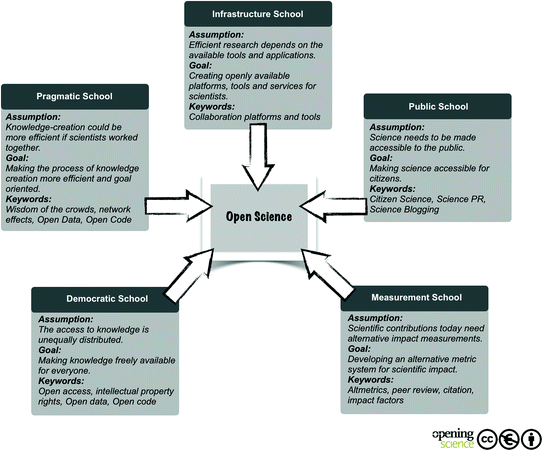
\includegraphics{ethos-of-open/img/image2_5_schools_of_open_science.png}

}

\caption{Five chools of open science: infrastructure, pragmatic,
democrratic, measurement, public school. Visit the paper for more
details on each.}

\end{figure}

Diverse practices, assumptions and goals are just part of the complexity
of open science. There are also divergent moral principles guiding open
science communities. Such principles are captured in 📖\emph{codes of
conduct}📖. A code of conduct is a community governance mechanism that
outlines the principles and practices expected of a given research
community's members, as well as the process for investigating and
reprimanding those in violation of the code.

In a sense, a code of conduct constitutes the moral backbone of a
research community. However, as with the numerous schools of thought,
there are similarly many codes of conduct. In other words, there is no
\emph{one} set of universal principles that all open science
practitioners abide by. For example, consider how
\href{https://openlifesci.org/code-of-conduct}{OLS},
\href{https://osf.io/6gsye}{INOSC},
\href{https://allea.org/portfolio-item/the-european-code-of-conduct-for-research-integrity-2/}{allea},
\href{https://www.agu.org/Plan-for-a-Meeting/AGUMeetings/Meetings-Resources/Meetings-code-of-conduct}{AGU}
and \href{https://ethicalsource.dev/community-code-of-conduct/}{Ethical
Source} all have different codes of conducts and guiding principles.

This great diversity responds to the growing proliferation of open
science initiatives and the great use we can make of open science
approaches to knowledge.

One of the biggest driving forces is the effect of open science on the
research performance. Indeed, some studies have even found that the
best-performing universities are those that conduct science following
open practices (see Huang et al.,
\href{https://doi.org/10.7554/eLife.57067}{2020}). More will be said in
the following lesson about the benefits of open science and different
stakeholders.

For now, consider some of the regional policies encouraging open
science:

\begin{itemize}
\tightlist
\item
  The European Commission
  (\href{https://data.europa.eu/doi/10.2777/121253}{2017}) has outlined
  the skills and competencies researchers need to practise open science;
\item
  The National Academies of Sciences, Engineering and Medicine
  (\href{https://doi.org/10.17226/25116}{2018}) promotes open science by
  design as a vision for 21st century research;
\item
  UNESCO
  (\href{https://unesdoc.unesco.org/ark:/48223/pf0000379949.locale=en}{2021})
  has developed a series of recommendations to ensure best open science
  practices, which are conducive to the United Nations'
  \href{https://sdgs.un.org/goals}{Sustainable Development Goals};
\item
  The European Open Science Cloud (EOSC) for finding and re-using data,
  and the Open Research Europe (ORE) publishing platform (European
  Commission, \href{https://data.europa.eu/doi/10.2777/18252}{2021}).
\end{itemize}

Ultimately, open science practices guide approaches to
knowledge-creation that best help confront the challenges of our era.
Through this module and the wider TOPS curriculum, you can become a part
of this impactful movement.

\hypertarget{performing-open-science-responsibly}{%
\section*{\texorpdfstring{Performing open science
\emph{responsibly:}}{Performing open science responsibly:}}\label{performing-open-science-responsibly}}
\addcontentsline{toc}{section}{Performing open science
\emph{responsibly:}}

\markright{Performing open science \emph{responsibly:}}

\textbf{Responsible Open Science} is a term we use through the rest of
the module. We define it as: considering open science as the core of
your science project and maximizing ethical actions for open science to
minimize current challenges (e.g.~data sharing, inclusion, and
accessibility). In responsible Open Science, the best possible and
practical practices should be explored at the early stage of your
science project.

Here we share with you following rules of thumb:

\begin{itemize}
\tightlist
\item
  Using best practices where possible
\item
  Being practical and realistic about resources available and pressures
  on open science practitioners
\item
  Not sharing things that shouldn't be shared
\item
  Being inclusive of all people
\end{itemize}

\hypertarget{summary}{%
\section*{Summary}\label{summary}}
\addcontentsline{toc}{section}{Summary}

\markright{Summary}

In this lesson, we have learned a brief history of open science, its
definition, and the ethos of open science and definition of responsible
Open Science. Open science practices provide significant advantages
relative to more traditional closed practices. However, there are still
problems that must be addressed, which many view as obstacles to open
science. In the next lesson, we will talk about the benefits of open
science and its challenges.

\hypertarget{further-reading}{%
\section*{Further Reading:}\label{further-reading}}
\addcontentsline{toc}{section}{Further Reading:}

\markright{Further Reading:}

Below are some further readings regarding this module:

\begin{enumerate}
\def\labelenumi{\arabic{enumi}.}
\tightlist
\item
  \href{https://link.springer.com/chapter/10.1007/978-3-319-00026-8_2}{Open
  Science : One Term, Five Schools of Thought}
\item
  \href{https://elifesciences.org/articles/16800}{How open science helps
  researchers succeed}
\item
  \href{https://nap.nationalacademies.org/read/26308/chapter/1}{Developing
  a Toolkit for Fostering Open Science Practices: Proceedings of a
  Workshop}
\end{enumerate}

National Academies of Sciences, Engineering, and Medicine. 2021.

\begin{enumerate}
\def\labelenumi{\arabic{enumi}.}
\tightlist
\item
  Reproducibility and Replicability in Science. Washington, DC: The
  National Academies Press. \url{https://doi.org/10.17226/25303} .
\item
  Open Science and Radical Solutions for Diversity, Equity and Quality
  in Research: A Literature Review of Different Research Schools,
  Philosophies and Frameworks and Their Potential Impact on Science and
  EducationGong, ``Open
  Science.''\url{https://doi.org/10.1177/20966083221091867}
\item
  Book by Miedema, Open Science.
  \url{https://doi.org/10.1007/978-94-024-2115-6}
\end{enumerate}

Further reading on terms and definitions:

\begin{enumerate}
\def\labelenumi{\arabic{enumi}.}
\tightlist
\item
  Open Science glossary from the FORRT (Framework for Open and
  Reproducible Research Training)
  \url{https://forrt.org/glossary/open-science/}
\end{enumerate}

\hypertarget{questionsreflection}{%
\subsubsection*{Questions/Reflection:}\label{questionsreflection}}
\addcontentsline{toc}{subsubsection}{Questions/Reflection:}

\hypertarget{questions-for-students-of-the-course}{%
\paragraph*{Questions for students of the
course:}\label{questions-for-students-of-the-course}}
\addcontentsline{toc}{paragraph}{Questions for students of the course:}

\begin{itemize}
\tightlist
\item
  How has research practice changed over the past few decades ?
\item
  As a researcher how do different components of responsible Open
  Science transform knowledge contribution?
\item
  We learned that there is ``no one ethos'' in this lesson. Can you
  explain what this means, and why?
\end{itemize}

\hypertarget{benefits-and-challenges-of-responsible-open-science-why-does-it-matter}{%
\chapter{Benefits and Challenges of responsible Open Science: Why does
it
matter?}\label{benefits-and-challenges-of-responsible-open-science-why-does-it-matter}}

\hypertarget{introduction-1}{%
\section{Introduction}\label{introduction-1}}

In the previous lesson, we learned about foundational concepts that
define Open Science. In this lesson, we address some benefits and
challenges of working in the open.

Here we aim to present a take on the development of science that's not
only focused on scientific results but also on the process of creation,
and the stakeholders that constitute the community.

Stakeholders can be individuals producing scientific knowledge (i.e,
researchers themselves), individuals consuming, applying and regulating
scientific research (i.e., practitioners, general public, policy-makers,
organizations, communities, etc.), and the larger scientific ecosystem
(i.e., scientific journals, repositories, archives, etc.). We discuss
more about the people who perform and benefit from open science - and
how to support them - in
\protect\hyperlink{stakeholders-of-open-science-who-practices-responsible-open-science-and-for-whom}{Lesson
3}.

In this lesson, we highlight the various benefits of open science across
multiple stakeholders, providing some examples that can be explored
further. Further, challenges in adopting open science practices are
explored.

\hypertarget{benefits-of-open-science}{%
\section{Benefits of Open Science}\label{benefits-of-open-science}}

\hypertarget{quality-of-research}{%
\subsection{Quality of research}\label{quality-of-research}}

For researchers, a primary benefit of increased transparency and
verifiability is that it allows readers and stakeholders to judge
whether results presented are accurate (Chambers, \& Tzavella, 2022)
and, importantly, that the results are not produced by questionable
research practices that lead to misleading or unreliable results (John
et al., 2012). Open science practices assure that various statistical
estimates of a study (e.g., p-values, effect sizes) can meaningfully be
interpreted (Mayo, 2017; Cummings et al., 2016). And allows others to
scrutinize the analytic decisions of the researchers, such as whether
the analysis was planned before or after observing the data (Nosek et
al., 2018). This allows others to check if they can arrive at the same
conclusion as the original research team, and facilitates stronger
public trust and support (UNESCO, 2021).

\hypertarget{real-world-implications-of-non-transparent-science}{%
\subsection{Real world implications of non-transparent
science}\label{real-world-implications-of-non-transparent-science}}

The Free Software Foundation Europe (FSFE) provides a compelling
position paper explaining why transparency is important for science.
When computers are used to produce scientific research, the code is
considered a ``method'', much like in a lab research setting, a set of
instructions for working with cells or agar plates might be a method.
Peer-reviewed methods are an essential step in the scientific process.
When these steps are not shared, no-one else can reproduce the work, or
build upon it for future scientific endeavors. It also allows people to
judge whether or not the methods are trustworthy.

In this case study, the FSFE reminds us of a time when closed methods
were not trustworthy. Volkswagen revealed it intentionally programmed
its diesel engines to cheat during laboratory emissions testing. This
meant that people drove these cars thinking they were trustworthy and
safer for the environment than they actually were. In this case, the
real emissions from the engines were more than 40 times over the legal
limit in the USA! Had the code for the diesel engines - the ``scientific
methods'' - been open, it is possible that this untrustworthy behavior
would have been picked up on much earlier.
\href{https://download.fsfe.org/policy/letters/20170105-horizon2020-position-paper.pdf}{(Gkotsopoulou
et al., 2017)}.

\hypertarget{quality-and-diversity-of-scholarly-communications}{%
\subsection{Quality and diversity of scholarly
communications}\label{quality-and-diversity-of-scholarly-communications}}

Furthermore, open science improves the state of scientific literature.
Scientific journals have traditionally faced the severe issue of
publication bias, where journal articles overwhelmingly feature novel
and positive results (Devito \& Goldacre, 2018). This results in a state
where scientific results in certain disciplines published scientific
results may have a number of exaggerated effects, or even be ``false
positives'' (wrongly claiming that an effect exists), making it
difficult to evaluate the trustworthiness of published results (Simmons
et al., 2011; Nissen et al., 2016). Open science practices such as
registered reports mitigate publication bias, and improve the
trustworthiness of the scientific literature. Registered reports are
journal publication formats that peer-review and accept articles before
data collection is undertaken, eliminating the pressure to distort
results (Chambers, \& Tzavella, 2022). Other open science practices,
such as 📖pre-registration📖 also allows allows a partial look into
projects that for various reasons (such as lack of funding, logistical
issues or shifts in organizational priorities) have not been completed
or disseminated (Evans et al., 2021) giving these projects a publicly
available output that can help inform about the current state of the
field.

\hypertarget{not-everything-should-be-pre-registered}{%
\subsection{Not everything should be
pre-registered}\label{not-everything-should-be-pre-registered}}

Pre-registration is the practice of registering your scientific
study/experiment plans before you start the study. This helps to ensure
that the experiment isn't changed part-way through if the results aren't
the conclusion the researchers had hoped for, and can help ensure
publication of ``null results'' which otherwise might not be published.

Pre-registration is a good tool for hypothesis-driven science, when a
researcher starts with a hypothesis, then proceeds to define steps
(methods) to prove or disprove the hypothesis. Not all science is
hypothesis-driven, though. Discovery driven science is more exploratory
and doesn't usually start with a hypothesis. It may instead involve
looking at existing data, or collecting more data, and trying to form
conclusions based on the available evidence. Many domains perform
discovery science, and generally these experiments and studies aren't
suitable for pre-registration, since the exact direction of study may
not be clear at the start of the research.

Open Science is also a valuable tool to be used in the public sector.
Movements like Public Money Public Code were started by people who
believe in the value of having open research and data freely available
to the population. Remarkable advances on the way we exerce democracy
are also being empowered by science made on the open, software like
Polis which leverages the concepts of Computational Democracy, empowers
scientists to run statistics and machine learning technologies on
opinions of millions of citizens. In other words, open science
facilitates 📖citizen science📖.

\textbf{Response to societal challenges}

As science tackles consequential topics (climate change, pandemics and
global health, democracy and misinformation), the transparency and
verifiability of science is more important than ever. This is
highlighted during the pandemic, where the creation of life-saving
vaccines were spurred because the genomic sequence of SARS-CoV-2 was
placed in GenBank, an open access database (Zastrow, 2020). Open science
allows for rapid, global access and action especially for shared
problems too difficult to solve by any one team alone.

Responsible Open Science is not only beneficial - it can also be
characterized as an ethical imperative, especially for publicly funded
projects. UNESCO (2021), for example, writes
``\hspace{0pt}\hspace{0pt}so as to ensure the human right to share in
scientific advancement and its benefits, member states should establish
and facilitate mechanisms for collaborative open science and facilitate
sharing of scientific knowledge while ensuring other rights are
respected''

The recent years have shown the great momentum of open science, with a
number of funders, regulatory organizations and governing bodies
mandating open science practices across various disciplines across the
globe (e.g.~European Commission; UNESCO, 2021; National Academies of
Sciences, Engineering, and Medicine. 2018 ), with more details about it
in Lesson 4 . The practicing scientist of today and especially of the
future needs to learn about open science and start applying it into
everyday practice.

\hypertarget{less-unnecessary-repetition-is-better-for-study-participants}{%
\subsection{Less unnecessary repetition is better for study
participants}\label{less-unnecessary-repetition-is-better-for-study-participants}}

Open science, in a way, also gives back to the communities that
scientists hope to serve. Through open science practices, research waste
can be avoided, such as unintentional and costly repetition of previous
studies (Lusoli and Glenos 2020). In the human sciences, this also
reduces participant fatigue in the long term. By maximizing what is
learned from publicly available data, one does not need to test
repeatedly especially on already vulnerable communities. By ``giving
away'' science, individuals, communities and organizations can more
easily adopt research results to inform interventions for their own
needs without the knowledge being gatekept by the original researchers
and organizations involved. In this way, open science can facilitate
strengthening the social and economic impacts of scientific results.

\hypertarget{personalcareer-benefits}{%
\subsection{Personal/career benefits}\label{personalcareer-benefits}}

Aside from accuracy, adhering to open science practices potentially
offers personal career benefits to researchers themselves. Openly
published research has a potential for greater visibility and impact by
reaching larger audiences across the internet, leading to more citations
and more like-minded collaborators and career/funding opportunities.
(McKiernan et al., 2016).

Open science practices can also enable stronger collaborations, both
within and between disciplines (Hormia-Poutanen, \& Forsström, 2016).
The ease of access to open data brings new agents to the landscape
allowing for broader and more diverse participation. Through open
science practices, such as pre-registration, one allows for a stronger
research design because feedback from various collaborators and
stakeholders can be solicited before data collection begins. Similarly,
preprints allow for speedier feedback on conclusions drawn from the data
once it is collected.

\textbf{Case study of a successful collaboration:}

\emph{Mozilla, an organization famous for the web browser Firefox, also
runs a community-driven project called Common Voice. Common voice is an
open crowd-sourced dataset of different voices and speech patterns,
covering many different languages, accents, countries, and speech
patterns. By making this data open and facilitating contributions from
volunteers worldwide, speech recognition technology and text-to-speech
technology is democratized and represents the members of the populace
more equitably.}

Practicing open science with transparency, collegiality, and research
integrity do require development of a whole set of technical and
transferable ``soft'' skills, which would be extremely useful for
researchers in their careers both in academic or non-academic sector.
Some examples include digital content creation; information,
publication, data literacy; communication and collaboration skills - we
will come back to it in the bonus section of lesson 5. Therefore, It is
important to have the training and mentoring widely offered to the
researchers.

\emph{Short on time? Make sure to read the top-ten reasons to do open
science at the end of this lesson for a quick TL;DR summary.}

\hypertarget{challenges-in-open-science}{%
\section{Challenges in Open Science}\label{challenges-in-open-science}}

However, open science also comes with its challenges. Doing open science
requires some extra effort from researchers to start and maintain, but
its long-term benefits include a great overall increase in research
efficiency, integrity, and public trust. For example, putting your code
in the open will probably mean that some adjustments must be made, and
sharing it with a community will demand that you choose how your
contributions can be used by others. Sharing data can imply extra work
and planning; however this organization and widespread discovery can
greatly improve science and confidence in it. We will see more details
on code sharing and licensing in the ``How'' lesson 5.

In this lesson we focus on the challenges of your work, and the
consequences of sharing - and in some cases, oversharing.

\hypertarget{not-everything-should-be-open---dont-overshare-without-consent}{%
\subsection{Not everything should be open - don't overshare without
consent!}\label{not-everything-should-be-open---dont-overshare-without-consent}}

In order to practice responsible Open Science, careful attention should
be given to how data is anonymized and how sensitive information is
removed from it in order to safeguard people's identity and to prevent
various harms stemming from breach of privacy. In recent history, we
have seen many cases of how the misuse of data and illicit means to
collect it is harmful to the population. Scandals like the
Facebook--Cambridge Analytica, and outrageous services selling very
personal parts of users' lives without their knowledge and full consent
are far too common. Preparing documentation, using standards, and
creating metadata takes time and effort

Additionally to treating users' data ethically, often further work is
required to make research outputs not only publicly available but also
understandable and accessible to various stakeholders. This means for
example, that codes to be shared are understandable and properly
documented. This might mean to have a testing system in place, make use
of a distributed version control software and a CI/CD pipeline. If
you're unfamiliar with any of these terms, don't worry! They will be
covered in the ``Open Software'' module. (Maybe this last sentence is a
cute little character with a balloon)

Besides caring about code, if the project utilizes data and that's being
open sourced, it might be necessary to also have documentation that
adequately describes the data set's contents, nature and layout. This
type of ``data about data'' is known as ``📖metadata📖''. It might also
mean to tweak the formatting of the dataset to fit a specific pattern
agreed by the broader community - this is known as using
community-agreed data standards.

\hypertarget{open-community-members-dont-always-agree-with-each-other}{%
\section{Open community members don't always agree with each
other}\label{open-community-members-dont-always-agree-with-each-other}}

Other than the more technical aspects of producing Open Science it's
also important to keep in mind the societal aspects of the project.
While interacting with the community can be one of the most fulfilling
things about Open Science, it might also be a source of disagreements
about the direction of the project or how it should be used. That's
where licenses and codes of conduct come into place. By explicitly
setting out rules for the community interactions and use of resources,
licenses and codes of conduct are useful to both protect the maintainers
and their vision of what the original project and the 📖forked📖
projects should comply with.

\hypertarget{case-scenarios-in-open-communities}{%
\section{Case scenarios in open
communities}\label{case-scenarios-in-open-communities}}

As you saw in the last lesson the story of Open Software (which builds
the foundation for Open Science) is vast and at times different open
values can conflict deeply. Two particularly relevant movements that
helped to shape our ideas and actions in Open Science today are the Open
Source and the Free Software movement.

The Open Source Initiative, an organization that advocates for Open
Source, argues that Open Source code can't ``discriminate against
persons, groups, fields or endeavors'', the Free Software movement
affirms that ``everyone should have the freedom to run the program as
they wish, for any purpose''. Even though these maxims might sound very
encompassing and welcoming there are several critics of the carelessness
that these movements have been treating both maintainers and users of
Open Source, as well as their gullible negligence on how powerful a tool
code is and how it can be used to do evil.

Speaking about doing evil, the Open Source Initiative addresses this
problem with these exact words ``Giving everyone freedom means giving
evil people freedom, too''. Recent movements like the Ethical Source and
the First Do No Harm movements have been questioning the broadness of
paradigms in which open resources are allowed to act, imposing ethical
restrictions to the use of software through the use of licenses. There
are also cases where the project maintainers took the lead and made
their own licenses, such as for the data format JSON.

Examples of open science and open source that have been used for
unintended purposes.

\begin{itemize}
\tightlist
\item
  ICE uses Chef-sugar (an open source project) {[}1{]} - an open source
  project being used by immigration enforcement authorities Illegal use
  of Elasticsearch branding by Amazon {[}2{]}{[}3{]}
\item
  All the ``what's bad'' essays on Stallman's website
\item
  📖Data Sovereignty📖, indigenous rights, and parachute/helicopter
  research: when marginalized people share their data, sometimes
  privileged researchers re-use the data without fair credit or funding
  reaching the original data creators.
\end{itemize}

Further, science that is just ``open'' does not necessarily mean that it
is of high quality. However, the transparency and verifiability that
open science affords, makes readers and various stakeholders able to
independently judge the trustworthiness of research products.

\hypertarget{cultural-barriers-not-everyone-wants-to-change-and-institutions-often-move-slowly}{%
\section{Cultural barriers: not everyone wants to change, and
institutions often move
slowly}\label{cultural-barriers-not-everyone-wants-to-change-and-institutions-often-move-slowly}}

A further challenge of adopting open science practices are institutional
barriers to the researcher or practitioner. While one might be
interested in adopting open science practices, they might lack support
from their department or project supervisors and open science practices
might not be given the budget, resources or time in a project cycle.
Institutions might also not recognize open science practices in
recruiting, training or promoting in the organization. These lack of
incentives within organizations present difficult barriers to the
adoption of open science.

While there are many challenges to the adoption of open science, we
believe that its various benefits and its ethical imperative to the self
and to the scientific communities, citizens and policy-makers outweighs
the cost of barriers. In addition, recognising the barriers and places
where caution needs to be taken provides a first step towards resolving
them.

\hypertarget{summary-1}{%
\section{Summary}\label{summary-1}}

Open Science provides benefits not only to society but also to the
individuals who perform it. Walking the line between responsible
appropriate sharing and irresponsible oversharing requires diligence but
the path and the results of science made in the open are very rewarding
to all its stakeholders.

\hypertarget{reasons-to-practice-open-science-responsibly}{%
\section{10 Reasons to practice open science
responsibly:}\label{reasons-to-practice-open-science-responsibly}}

\hypertarget{responsible-open-science}{%
\subsection{responsible Open
Science\ldots{}}\label{responsible-open-science}}

\begin{itemize}
\tightlist
\item
  \ldots{} (including availability of data, code, materials, and early
  results) accelerates research broadly and greatly.
\item
  \ldots{} generates transparency and public trust and support
\item
  \ldots{} fosters working across and engaging multiple disciplines, or
  ``convergent'' science.
\item
  \ldots{} brings innovation through using big and aggregated data and
  information
\item
  \ldots{} supports public and community uses of science: also known as
  community science, participatory science, or citizen science.
\item
  \ldots{} helps fight misinformation and disinformation
\item
  \ldots{} is intentionally and thoughtfully inclusive practice
\item
  \ldots{} supports the key role of science in addressing major societal
  challenges in the 21st century (including climate change,
  sustainability)
\item
  \ldots{} makes your research more efficient and impactful and provides
  credit broadly responsible Open Science is the new normal,and
  regulatory and governing bodies are reaching a consensus toward
  pushing it).
\end{itemize}

\hypertarget{questionsreflection-1}{%
\section{Questions/Reflection:}\label{questionsreflection-1}}

\begin{itemize}
\tightlist
\item
  Why are responsible Open Science practices important to a researcher's
  profile?
\item
  How can a researcher benefit from responsible Open Science practices?
\item
  How does society benefit from responsible Open Science?
\item
  In this lesson, we learned that responsible Open Science often takes
  time and requires diligence and dedication of researchers. Can you
  explain how and why?
\end{itemize}

\hypertarget{stakeholders-of-open-science-who-practices-responsible-open-science-and-for-whom}{%
\chapter{Stakeholders of Open Science: Who practices responsible Open
Science and for
whom?}\label{stakeholders-of-open-science-who-practices-responsible-open-science-and-for-whom}}

\hypertarget{introduction-2}{%
\section{Introduction}\label{introduction-2}}

In previous lessons, we learned about the concept and motivation and
aspiration of open science. Now let's think about ``who'' is practicing
open science and for whom. In the first section of this lesson we dive
deeper into understanding who the stakeholders for Open Science are. In
the second part we cover essential topics about barriers to
participation, and to include diverse stakeholders in open science
communities and ways to overcome them.

In this module we offer you a person-centered approach to making open
science happen. Our intention is to prevent harmful consequences of
science's misuse (even unintentional misuses) and to increase the impact
of science, by leveraging other researchers' works and improving
society.

\hypertarget{who-performs-and-benefits-from-open-science-stakeholders-partaking-in-open-science}{%
\section{Who performs and benefits from open science? Stakeholders
partaking in open
science}\label{who-performs-and-benefits-from-open-science-stakeholders-partaking-in-open-science}}

As briefly discussed in previous lessons, Open science doesn't only
concern researchers; many other stakeholders are affected by the
outcomes of open science as well. Stakeholders are any individuals who
can affect or be affected by open science projects. Although there are
different ways to categorize stakeholders depending on your science
projects, mainly there are three large groups; 1. Researchers, 2.
Public, and 3. Policy-makers.

\begin{itemize}
\tightlist
\item
  Researchers
\item
  Organizations
\item
  Research Teams
\item
  General public
\item
  Decision Makers (regulatory, funding bodies, etc)
\item
  Government
\end{itemize}

\hypertarget{researchers}{%
\subsection{Researchers}\label{researchers}}

Individuals engaged in creating new knowledge (e.g.~researchers,
students, faculty staff at universities, researcher centers, researchers
at libraries). Responsible for creating an open science environment as
well as open outputs and processes.

\hypertarget{public}{%
\subsection{Public}\label{public}}

Lay people who can drive/improve/conduct science (i.e.~people who may
not have an academic background or research experience). This may also
be referred to as ``citizen science'', but you do not have to be a
citizen of any particular country in order to participate in science!

\hypertarget{policy-makers}{%
\subsection{Policy-makers}\label{policy-makers}}

Those with decision-making power (e.g.~government, regulatory bodies)

\hypertarget{how-each-group-contributes-to-open-science}{%
\section{How each group contributes to Open
Science}\label{how-each-group-contributes-to-open-science}}

Let's take a look at these groups, how they can contribute to open
science (input) and what benefits they experience from open science
(this was also discussed in Lesson 2). Note that overlap among
researchers, the general public, and policy-makers can happen.

Researchers' contribution to open science manifests by sharing and
communication their research via open access publications (more about it
in the Lesson How and Module Open Results) As a result, community of
researchers benefits from increased visibility and credit,
reproducibility, access to more data and attraction of funding, reduced
work's duplication, conservation of resources and increased
accessibility

The general public contributes to open science research by above
mentioned ``citizen science'' projects, as e.g.~as volunteers to collect
or manage (e.g.~categorize) some type of data.

As a result, individuals boost their understanding of science and feel
empowered by having opportunities to exert influence. Disinformation in
the public arena is decreased, and the routes of access to trustworthy
sources of information are strengthened.

Policy-makers play important role in ensuring and facilitating open
science by setting data management processes, open access legislation,
developing ethical guidelines for experiments As a result, higher
quality of research done with open science principles and efficient
communication between stakeholders leads to better-informed decisions

This figure briefly shows how three groups of stakeholders interact with
each other. Healthy interactions will foster respect and overcome power
dynamics. Each group should focus on empowering other groups and be
aware that open science cannot exist without the others. Resources and
tools for interactions are described in greater detail in Lesson 5, (and
in the tools and results modules).

\hypertarget{case-scenarios}{%
\section{Case scenarios}\label{case-scenarios}}

Now let's take a look at examples of successful interactions around the
world!

\hypertarget{case-scenario-1-trend-public-policy-makers}{%
\subsection{Case Scenario \#1: Trend: Public ---\textgreater{}
Policy-makers}\label{case-scenario-1-trend-public-policy-makers}}

The public has many opportunities to join research projects and can play
prominent roles in science. There are more than 30 ways to define
Citizen Science (Haklay et al., 2021), and the principle is ``active
public involvement in scientific research'' (Irwin, 2018). Citizen
Science contributes to policy making at various stages of the policy
cycle, including policy preparation, formulation, implementation,
monitoring, and evaluation Scade et al (2021). That is to say, citizens
are capable of setting trends and informing the directions in policy
making.

In 2015, the United Nations adopted the 2030 Agenda for Sustainable
Development for peace and prosperity for people and the planet, now and
into the future (United Nations, 2021). This agenda has 17 specific
goals that require a large amount of data. Citizens have been
contributing by providing the water and air quality, marine litter,
biodiversity, health, and gender issues data (Fritz et al, 2019), and
Scade (2021) describe this as '' a source of information for policy
making.'' This is a powerful example of citizens influencing global
policy trends.

\hypertarget{case-scenario-2-officialize-policy-makers-researcherspublic}{%
\subsection{Case Scenario \#2: Officialize:
Policy-makers---\textgreater{}
Researchers/Public}\label{case-scenario-2-officialize-policy-makers-researcherspublic}}

Policy-makers can implement new regulations for both researchers and the
public. Bothwell and Smith (2017) reported that policy can shape
knowledge. For example, policies such as dispersion of research funding
(i.e.~which science disciplines including Citizen Science receive the
most funding), and data management plans for the public can impact the
amount of knowledge produced.

Most importantly, policy-makers are mindful that researchers and citizen
scientists conduct science projects safely and ethically. National
Institute of Health (2022) states that policy sometimes sets the rules
of the road for conducting research, helping ensure that scientific
investigations are carried out safely, securely, adhering to the highest
standards of research integrity, and in a way that addresses evolving
ethical concerns. We can find these ethical policies, for example, NIH
Guidelines for Human Stem Cell Research. Some countries have legislation
requiring research to be published openly, such as Spain's open access
legislature. Policies on open access for European countries are
monitored and reported by corresponding OpenAire National Open Access
Desks.

\hypertarget{case-scenario-3-participate-public-researchers}{%
\subsection{Case Scenario \#3: Participate: Public
---\textgreater Researchers}\label{case-scenario-3-participate-public-researchers}}

Currently, NASA has 28 Citizen Science projects that are open to people
around the world (NASA, 2022). According to NASA Citizen Science policy,
Citizen Science is defined as a form of open collaboration in which
individuals or organizations participate voluntarily in the scientific
process in various ways. The projects vary from Earth and planetary
science to biological science such as researching meteorites, mosquitos,
and the surface of Mars.

One of the evaluation criteria for NASA Citizen Science is; two-way
communication between volunteers and NASA scientists and including
diverse citizen scientists, with scientists giving feedback to and
receiving feedback from the volunteers (NASA SMD Policy Document SPD-33,
2018). Also NASA creates opportunities for citizen scientists to be
co-authors for publications and 191 NASA Citizen Scientists joined
scientific publications since 2011 (NASA, 2022).

In addition to citizen science, there is an emerging concept called
community science and co creation. Community science refers to science
projects that honor community priorities. They can be initiated by a
science practitioner or a community member, but they must become a
collaborative endeavor (ASTC, 2021). Co-creation in science refers to
the collaboration between a variety of actors (people from different
societal roles) actively joining forces to tackle jointly defined
challenges (Stier and Smit, 2021). We can also state that community
science, which prioritizes community needs, succeeds through efforts of
co-creation.

Charles et al (2020) introduced a successful case of community science.
One example is protecting one of the remote islands in Canada that is
facing the threats of sea level changes (e.g.~salt water intrusion to
groundwater and losing archaeological sites). As a result of community
science and co-creation through public, universities, and policy makers,
now climate-related mapping and visualization techniques for
vulnerability assessments are available for use within the community.
This provides opportunity for all the residents to explore adaptation
options to ongoing sea level changes. The community was also able to
work with archaeologists on preservation initiatives.

\hypertarget{case-scenario-4-share-researchers-policy-makerspublic}{%
\subsection{Case Scenario \#4: Share: Researchers
---\textgreater Policy-makers/Public}\label{case-scenario-4-share-researchers-policy-makerspublic}}

About 2,000 researchers work together to create a report for the
Intergovernmental Panel on Climate Change on the current situation,
which is a technical report that most people would have trouble
understanding (Woolston, 2016). Some climate researchers break down
their results to explain to policy-makers and citizens. Policy makers
can utilize the results to officialize the restriction of CO2 emission
level (e.g.~Paris Agreement) and the public can be aware about what they
can do in their daily lives to achieve the CO2 emission goal. This shows
that each group is playing a significant role in addressing the climate
science project, which is considered as one of the critical issues that
our generation is facing.

\hypertarget{how-diverse-stakeholders-are-included-in-open-science}{%
\section{How diverse stakeholders are included in open
science:}\label{how-diverse-stakeholders-are-included-in-open-science}}

Stakeholders are incredibly diverse in terms of culture, communication,
and ability. To make science truly open, we must ensure that open
science is accessible to everyone, so that we can all fully participate
and benefit from the work. The best way to include stakeholders is to
remove existing barriers and design for inclusion.

Creating a more inclusive environment will both increase the amount of
people who feel welcomed to contribute back to your research and will
broaden the scope of people that can comprehend and interact with the
products of the research. Small actions towards conforming to
accessibility and diversity guidelines will go a long way towards making
your work truly open to all, maximize the visibility and impact of
research..

Let's look at some factors and potential barriers for participation in
the open science, with possible solutions:

\hypertarget{socioeconomic-status}{%
\subsection{Socioeconomic status:}\label{socioeconomic-status}}

Instabilities in the electric, electronic and internet access
(e.g.~load-shedding, internet speed, electronic device performance)

\textbf{Possible solution(s):} open science materials and communication
channels should require less resources whenever possible

\hypertarget{neurodivergence}{%
\subsection{Neurodivergence:}\label{neurodivergence}}

Diversity of neural architecture leads to different learning and
socialization styles

\textbf{Possible solution(s):} employ multimodal communication
strategies using different visual and audio outputs, varied pace of
events and conversations

\hypertarget{disabilityimpairments}{%
\subsection{Disability/impairments}\label{disabilityimpairments}}

\begin{itemize}
\tightlist
\item
  Sensory - e.g.~colorblind, blind, deaf, auditory and/or visual
  processing conditions
\item
  Physical - e.g.~conditions that affect energy levels, neuromuscular
  coordination conditions
\item
  Mental - conditions that affect mental health (e.g.~depression,
  schizophrenia, etc)
\end{itemize}

\textbf{Possible solution(s):} employ multimodal strategies and
universal design to provide proactive accommodations for as many as
possible - captions, transcripts, colorblind-friendly palette, document
formatting that are compatible with screen readers, normalizing flexible
work schedules and rolling deadlines with collaboration

\hypertarget{intersecting-identities-and-intersectionality}{%
\subsection{Intersecting Identities and
intersectionality}\label{intersecting-identities-and-intersectionality}}

Epistemic oppression - e.g.~dominance of English as the international
language for all science. Non-native English speakers are disadvantaged
by default.

\textbf{Possible solution(s):} Proactive translation of open science
results/communications in other languages

\hypertarget{microaggressionsmacroaggressions}{%
\subsection{Microaggressions/macroaggressions:}\label{microaggressionsmacroaggressions}}

Use of words with negative connotations towards individuals and groups
and negative behavior/ostracization

\textbf{Possible solution(s):} Employ language and communication with
neutral connotations that do not use pejorative terms or vilify a group
(example) in biology, we use males to identify the parent with testes
and the female with ovaries; should change language to ``parents with
testes/ovaries'' etc) Gender Inclusive Biology for more detail

\textbf{⚠️ Caution:} Full participation in open science requires respect
of an individual's identity, autonomy, and lived experiences.
\emph{Microaggressions, macroaggressions, and epistemic oppression are
identity barriers to open science.}

This list is not comprehensive, but is meant to be a starting point in
preparing your work in open science for diverse stakeholders.

\hypertarget{activityexercise}{%
\section{Activity/exercise}\label{activityexercise}}

Now let's practice by looking at some typical case scenarios and
solutions, reflecting on things you could do for inclusion:

\hypertarget{case-scenario-1-accessible-figures-and-writing}{%
\subsection{Case Scenario \#1: Accessible figures and
writing}\label{case-scenario-1-accessible-figures-and-writing}}

You have finished your project and are busy typing your paper to submit
to an open science preprint journal. In your paper, you have several
figures that use multiple colors at once - red, green, and blue. In
addition, you have formatted your paper to use a serif font at size 10.
\textbf{You want to make sure that your paper is easily readable for
everyone. What are some things you can do?}

\begin{itemize}
\tightlist
\item
  Colorblind people have high difficulty with red, green, and blue
  colors. You can check your figures by running a color blind simulator,
  e.g.~open source RGBind. Consider using colorblind-friendly palettes
  with colors such as green, magenta, and others. Avoid using color hues
  to convey information if at all possible.
\item
  Legally blind and dyslexic people have difficulty with font size and
  font types. Consider using a font size of 12 or higher, and use a
  `Sans-Serif font' such as Arial or Verdana to assist people with
  dyslexia in reading your manuscript.
\end{itemize}

\textbf{Bonus question:} What should you do if a journal insists on
using a font size and font type that is inaccessible to some people?

\hypertarget{case-scenario-2-organizing-an-inclusive-physical-event}{%
\subsection{Case Scenario \#2: Organizing an inclusive physical
event}\label{case-scenario-2-organizing-an-inclusive-physical-event}}

You are the head organizer for an open source code hackathon for your
organization. Your boss initially suggests using the large seminar room
with one projector and screen that is hard to see from the back of the
room. When starting the hackathon, you find out that a couple of
attendees are deaf and a couple of other attendees have visual
difficulties. What are some quick things you could do to help them fully
participate in the hackathon?

\begin{itemize}
\tightlist
\item
  If doing a presentation on Powerpoint, you can turn on `Always use
  subtitles' for live transcription. Check if your font size on your
  presentation is large enough to comfortably see at the back of the
  room.
\item
  If possible, consider simulcasting the presentation on Zoom or other
  virtual platform with captions/transcription.
\item
  Use text for communicating with deaf attendees.
\end{itemize}

\hypertarget{case-scenario-3-organizing-an-inclusive-virtual-meeting-and-preparing-in-advance}{%
\subsection{Case Scenario \#3: Organizing an inclusive virtual meeting
and preparing in
advance}\label{case-scenario-3-organizing-an-inclusive-virtual-meeting-and-preparing-in-advance}}

You are organizing a virtual open science meeting with established and
prospective members from different countries. You are unsure of what the
prospective members need in order to participate fully, and no one
emailed you to let you know about accommodations they need. What should
you do?

Being proactive with small things you can do ahead of time by
implementing some of the accommodations before the meeting (see possible
solutions to barriers that we have just considered). While it is
difficult to preconceive every possible accommodation that you might
need to provide for your members, if you communicate your willingness to
do everything you can to help members thrive, you are doing incredibly
important work to not only recruit prospective members to open science,
but also to retain them.

\textbf{Bonus tip:} Subtitles and closed captioning are not only for
deaf/hard-of-hearing people, they are also very beneficial for
non-native English speakers to understand the conversation fully.
Consider using a third-party app such as otter.ai for accurate closed
captioning and simultaneous transcripts that can be saved for members to
read through.

\textbf{What are some other accommodations that could be useful for
everyone in general?}

\hypertarget{summary-2}{%
\section{Summary}\label{summary-2}}

In the first part of this lesson, we learned about the types of
stakeholders and how they can interact to empower each other. Successful
examples were introduced, and you can reflect and analyze how to develop
these interactions in your science projects. These arrangements may
initially take time, but the outcome is essential to advance science,
and is also rewarding.

In the second part of the lesson, we studied how diverse stakeholders
can be included in open science with case scenarios designing for
inclusion. Taking measures to maximize diversity, inclusion, and
accessibility of your science project will enrich the project, boost its
visibility and engagement of participants. Healthy interactions among
stakeholders with diverse members creates the strength of science
projects and rewarding results, and a diverse team drives innovation to
success. Remember that what you learned here is not an optional choice
but an integral part of responsible Open Science.

To learn more about joining, contributing to, and creating your own
communities, consider visiting the Tools module.

\hypertarget{questionsreflection-2}{%
\section{Questions/Reflection:}\label{questionsreflection-2}}

\begin{itemize}
\tightlist
\item
  What steps can you take to make these open science resources more
  inclusive?

  \begin{itemize}
  \tightlist
  \item
    Written resources and images
  \item
    Conferences - virtual, physical, or hybrid
  \end{itemize}
\item
  Communication with the general public and policy makers should not be
  something that researchers only do when they have spare time, after
  the research is done and published. It should be treated as a critical
  part of a science project, to certain extent at all stages of
  development Explain multiple possible communication channels and
  strategies for researchers, and why each is important.
\end{itemize}

\hypertarget{impact-of-open-science-on-academia-communities-and-society-as-a-whole-where-open-science-happens.}{%
\chapter{Impact of Open Science on academia, communities and society as
a whole: Where open science
happens.}\label{impact-of-open-science-on-academia-communities-and-society-as-a-whole-where-open-science-happens.}}

\hypertarget{introduction-3}{%
\section{Introduction}\label{introduction-3}}

We have so far explored the fundamental parts of what Open Science is:
why to pursue it and who the stakeholders of open research are. Where
you are in the world when performing open science can have an impact on
how you perform it, too. Laws across the world vary, and the advantage
of open science means people from around the world can participate,
co-create, and consume content together. This can affect your work from
social and legal perspectives, and may present technical challenges as
well.

Legal frameworks that affect responsible Open Science Open Science
promises to make research work more accessible, all-encompassing,
participatory, understandable and re-usable for wider audiences. Keep in
mind, making the process open does not in itself result in wide
participation unless it's partnered with sufficient financial resources,
technological advancements, knowledge and skills. It's important that
all these are available across regions, institutions and
socio-demographics (review by Hellauer et al.~2022)

\hypertarget{data-protection-privacy-and-data-sovereignty}{%
\section{Data protection, privacy, and data
sovereignty}\label{data-protection-privacy-and-data-sovereignty}}

\textbf{⚠️Caution:} To perform open science responsibly, it is important
to consider not only what you should share, but also what not to share.

Individuals may have a right to privacy in their communications, for
medical records, and for their physical locations. Similarly, certain
countries, communities, and especially Indigenous peoples may
historically have been exploited, and may wish to retain more rights
over their knowledge to protect from further exploitation. Globally,
there are laws around the world that may cover some of these issues, but
not all countries and regions have equal levels of protection, and some
have none at all.

We share some case studies:

\hypertarget{european-case-general-data-protection-regulation}{%
\subsection{European case: General Data Protection
regulation}\label{european-case-general-data-protection-regulation}}

There are protective laws and legal frameworks in certain places around
the globe that affect open science. European researchers have to abide
by the General Data Protection regulation (GDPR) while making a data
sharing statement stating the non-availability of data sharing. This
hinders sharing particular data. Here, the scientific society should
come forward to allow responsible Open Science data sharing
possibilities in the global scientific space (Giske Ursin \& Heidi Beate
Bentzen, 2021)

\hypertarget{south-african-case-protection-of-personal-information-act-popi-act-and-open-science}{%
\subsection{South African case: Protection of Personal Information Act
(POPI Act) and Open
Science}\label{south-african-case-protection-of-personal-information-act-popi-act-and-open-science}}

The POPI Act No.~4 of 2013 is regulation by the government of South
Africa to safeguard the personal information of South African citizens,
like the General Data Protection Regulation (GDPR) in Europe. The
regulation states that if one is obtaining personal information of South
African citizens through phones, focus groups, interviews, containing
identifiers such as names, contact information then you have to be POPI
Act compliant.

In the research context, one needs to make sure that if the personal
identifiers are collected then they must not be shared with third
parties and stored securely in an access-controlled location to prevent
a data breach. The act doesn't impede open data sharing, but personal
identifiers should be removed from shared datasets. The POPI act affects
the research process, in a way to make sure that storing of data of only
de-identified datasets on cloud storage \& onsite data storage is
strictly controlled to specific designated individuals to ensure data
safety (POPIA Code of Conduct for Research, 2021).

\hypertarget{united-states-case}{%
\subsection{United States case:}\label{united-states-case}}

In the United States, there is no federal-level legislation similar to
POPI or GDPR, but there are some state-level laws, such as the
California Privacy Rights Act, and the Virginia Consumer Data Protection
Act.

\textbf{📝 Exercise:} Check what laws, if any, apply in your state.

\hypertarget{summary-working-in-a-global-society-with-varied-data-protection-laws}{%
\subsection{Summary: Working in a global society with varied data
protection
laws}\label{summary-working-in-a-global-society-with-varied-data-protection-laws}}

Given the broad variation of data protection laws around the world, it
may seem tricky to navigate. By practicing responsible Open Science,
however, our response can get a little bit clearer. We can consider
relevant legislation (if any) to be a bare minimum, and instead ensure
that we are involving relevant stakeholders, as discussed in lesson 4,
and listening to their needs respectfully, even if it means we are more
cautious than local legislation may require.

\hypertarget{whose-laws-apply-to-my-community}{%
\section{Whose laws apply to my
community?}\label{whose-laws-apply-to-my-community}}

Social, cultural, and legal norms will vary from country to country, and
international communities. Avoiding culture clashes can be made more
manageable by setting out explicit cultural norms for your community,
such as may be specified in a code of conduct, which we discussed in
lesson one of this module. Try to avoid assumptions that tie to a
specific physical location or culture. Some examples why this is
important:

\begin{itemize}
\tightlist
\item
  Laws are not uniform. If activity X is legal to do in one country, but
  not another, a code of conduct which says ``obey the law'' becomes
  impossible to interpret fairly or to enforce.
\item
  Hosting a conference in a country that doesn't have strong human
  rights records might result in someone breaking the law by being
  LGBTQIA+, or by not wearing religious garb.
\item
  ``We plan to release this in the summer'' might be clear if you're all
  in the same country, but if your collaboration is spread across the
  northern and southern hemisphere, is summer in the middle of the year
  or the end of the year? Consider using a month name instead - ``we
  plan to release this by March'' is unambiguous.
\end{itemize}

\hypertarget{equity-and-open-science}{%
\section{Equity and Open Science}\label{equity-and-open-science}}

Many countries in Asia, Africa and Latin America face many challenges,
including lack of funding, inadequate access to literature and poor
infrastructure. Across these regions, young scientists are working to
build practices for open science from bottom-up. The aim is that
scientific communities will incorporate these principles as they grow
but these communities' needs differ from those that are part of mature
research systems.

The reasons for falling behind are lack of funding, poor infrastructure,
inadequate access to research resources. There are government policies,
which want greater productivity at the expense of quality. The open
science collaborations can bridge the gap for developing countries by
providing new ways and provide researchers access that might be
currently out of reach (Onie, S. 2020).

\hypertarget{equitable-terminology-what-words-should-we-use}{%
\subsection{Equitable terminology: what words should we
use?}\label{equitable-terminology-what-words-should-we-use}}

When talking about equity from a global perspective, it can be very hard
to choose appropriate language, and historically many phrases have come
and gone as we learn more equitable ways to communicate. Common phrases
you may see include ``Higher Income Country'' and ``Lower or Middle
Income Country''. These are terms defined by the World Bank. Some people
prefer to use ``Global North'' when referring to more privileged / high
income countries, and ``Global South'' for lower income / more exploited
and marginalized countries - but some ``Global South'' countries are in
the northern hemisphere, and vice versa! Other times, people use
``minority'' and ``majority'', but again sometimes the phrase
``minority'' might be used for a populace that is not actually a
minority! An older phrase is ``first world country'' or ``third world
country''. Many of these terms also have accidental or intentional
negative connotations. For this module, we aim to use the phrases
``marginalized'' and ``privileged'' when referring to the inequitable
distributions of resources and power amongst humanity.

The Global North have ascendency over authorship and synergies in
research networks, which margins out the Global South (Cash-Gibson L et
al 2018).

In richer regions, a compulsion for the goal of excellence nurtures
cumulative benefit in funding allocation for the highest funded
institutions (Noble P et al) Across many countries, very few women have
higher positions, senior positions are given at a later age, given less
grant funding and few have high-impact publications (Gesiarz F et al
2020) (Brown JVE et al 2020 ) These are the impartialities, which are
the societal imbalances (Zuckerman H. (1988). The above stated societal
imbalances, which Open Science is focused to minimize in order to
elevate the underrepresented societies, groups and create avenues for
Global South countries to come forward \& contribute to the global
science community.

Prainsack \& Lionello (2018) stated that open science is a political
assignment greater than its technological part. The Open Science policy
in Europe is shifting across nations, institutions \& funding
organizations. (Sveinsdottir T et al 2020). The emphasis on policies
drive the incentive/reward structures and resource allocation and later
helps in establishing strategies. Open Science started as a bottom-up
approach by the researchers but has gone to the top-end level making it
to the national and institutional policies setting wider goals like
economic growth. The European Commission favors Open Science but in 2016
EU publication, the concern of Open Science perceived potential is being
given that greater importance for fostering Europe's competitive
advantage in global markets (link to EU publication, 2016) Open Science
positions to cover literature in languages other than English,
supporting the value of 📖bibliodiversity📖. We see a diverse set of
communities in organizations working for Open Science data, software,
tools, resources together as multilingual teams' covering different
languages of the world. Research indicates that there is a demand for
regionally focused titles, in regional languages (Snijder 2022)..

\hypertarget{a-global-perspective-on-open-science}{%
\section{A global perspective on open
science}\label{a-global-perspective-on-open-science}}

\hypertarget{unesco-on-open-science-infrastructure}{%
\subsection{UNESCO on Open Science
Infrastructure}\label{unesco-on-open-science-infrastructure}}

UNESCO's recommendation on Open Science states the potential of open
science is in minimizing the present inequalities in Science, Technology
and Innovation and pace towards SDGs 2030 implementation agenda,
specifically in Africa, least developed countries, small island
developing states and landlocked developing countries.

Open Science infrastructures are shared infrastructures (referred as
virtual/physical, knowledge-based resources such as journals,
collections, and open access publication platforms, archives,
repositories, scientific data, present research informations systems,
sets of instruments, open bibliometrics, scientometrics systems for
assessing \& analyzing scientific areas, open computational \& data
manipulation service infrastructures, multidisciplinary data analysis \&
digital infrastructures) where open science happens and serves the needs
of diverse communities. Please see UNESCO Recommendation on Open Science

UNESCO on Open Science policies clearly recommends monitoring Open
Science through combining qualitative and quantitative methods to assess
the efficacy and efficiency of Open Science as per the member states'
particular conditions, constitutional structures and constitutional
provisions. Also, gathering \& communicating progress, good practice,
research work \& innovation in open science and its outcomes with
support of UNESCO and diverse stakeholders approach.

\hypertarget{organisation-for-economic-co-operation-and-development-oecd-and-open-science}{%
\subsection{Organisation for Economic Co-operation and Development
(OECD) and Open
Science}\label{organisation-for-economic-co-operation-and-development-oecd-and-open-science}}

The OECD's recommendation regarding research data from public funding
helped gain collaboration and global sharing of data as a policy
priority, with the objective of making the global science system more
effective and seamless. There has been progression in a number of OECD
member states and partner economics, with 58 countries successfully
delineating their policies for open data \& research publications. - For
IT infrastructure, academic institutions and data repositories,
international networks have been established in the form of repository
networks such as OpenAIRE. - ``Science clouds'' - national and
international computational resources - are being initiated such as
European Open Science Cloud, the Australian cloud NECTAR, the National
Research Data Infrastructure in Germany, the National Institute of
Health Data Commons in the USA \& Research Center for Open Science and
Data Platform in Japan.

\hypertarget{questionsreflection-3}{%
\section{Questions/Reflection:}\label{questionsreflection-3}}

\begin{itemize}
\tightlist
\item
  What strengths do marginalized communities bring to open science? What
  challenges may they face compared to privileged communities?
\item
  Name at least one data privacy law, and describe ways you can keep
  personal data safe. Do all countries have data privacy laws?
\item
  Bonus: You're working on an open science consortium that gathers data
  in the Netherlands, Kenya, and India. You plan to use servers in the
  EU to store your data. What concerns should you take into account?
\end{itemize}

\hypertarget{not-an-afterthought}{%
\chapter{Not an afterthought}\label{not-an-afterthought}}

Previous lessons have shown the importance and benefits of open science,
presented some key stakeholders involved, and discussed the barriers to
participation and ways to overcome them. This lesson will guide you in
how to start infusing responsible Open Science in your own work, which
might be independent, or could be in a research group or lab.

\hypertarget{plan-for-open-science-into-the-design}{%
\section{Plan for open science into the
design}\label{plan-for-open-science-into-the-design}}

Practicing responsible Open Science requires organizing your work and
research, and your team, if you have one, around open science and
planning for it from the inception, even designing the project with open
science in mind. There are many resources and tools that make these
easy, and indeed doing so will improve efficiency and the value and
impact of your work, and help you focus on your research itself. We'll
provide a brief overview in this lesson, but you may wish to explore the
later modules in this course too, which cover 🔗 Open Data, Open
Results, Open Tools, and Open Software 🔗. Additional resources, and
knowledge, may be available at your institution, including in your
department or library or among your colleagues. An additional resource
is a recent report from the U.S. National Academies
``\href{https://nap.nationalacademies.org/catalog/25116/open-science-by-design-realizing-a-vision-for-21st-century}{Open
Science by Design}.''

It is important to discuss responsible Open Science with your research
team, lab, group or partners regularly. Much of responsible Open Science
may seem to be related to outputs -- such as data, software, and
publications -- but preparing and organizing work for these in advance
is critical. It would be hard or impossible to follow leading practices
for these at the end of research, in the ``afterthought'' mode.
Responsible Open Science is both a mindset and culture.

Planning for outputs in advance includes: speaking about it and
organizing with your research team; deciding which tools to use;
thinking about authorship and credit; engaging with relevant
stakeholders and research partners, for example, industry, around open
science; identifying repositories for software and data; highlighting
these approaches in your grant; and much more.

\hypertarget{perks-of-digital-and-internet-age-for-responsible-open-science}{%
\section{Perks of digital and internet age for responsible Open
Science:}\label{perks-of-digital-and-internet-age-for-responsible-open-science}}

The internet has made it very easy to share digital work. The
popularization of Open Source computer code and the rise of Open Science
has resulted in many outlets for public and free hosting of research and
data.One key to open science, and why it is so empowering for 21st
century science, is that we can now connect all the participants,
stakeholders, and outputs of a research result together so that they are
easy to discover.

Here we present a non-exhaustive list of digital platforms and tools
used with for open science:

\begin{itemize}
\tightlist
\item
  Digital Persistent identifiers - for objects and researchers (such as
  doi and ORCID)\\
\item
  \href{https://pkp.sfu.ca/ojs/}{Open Journal System}: open source
  software for managing \& publishing scholarly journals\\
\item
  Electronic notebooks such as \href{https://jupyter.org/}{Jupyter} and
  \href{https://rmarkdown.rstudio.com/}{R Markdown}\\
\item
  Data repositories: genetic sequence database
  \href{https://www.ncbi.nlm.nih.gov/genbank/}{Genbank}, protein data
  bank (\href{https://www.rcsb.org/}{PDB}), Dataverse, figshare, Zenodo
  and for wide search use \url{https://www.re3data.org/} and/or
  \url{https://datacite.org/}\\
\item
  Softwares/Codes: Zenodo used with Github / mybinder\\
\item
  Materials: Addgene (for molecular biology)\\
\item
  Reference management tools: Zotero, Mendeley\\
\item
  Academic Social networks: Academia.edu, ResearchGate\\
\item
  Peer Review: Publons, PreView\\
\item
  Project management: Open Science framework
\item
  Github as a platform for collaborative work on training materials etc
\end{itemize}

A variety of tools are emerging to help manage open science workflows,
and to support global collaboration. These include spaces for project
management, such as the Open Science Framework from
\href{https://www.cos.io/}{Center for Open Science, electronic}
notebooks which help projects organize data, software, and content
together; online platforms for creating manuscripts, etc. More
information about the open science collaboration and management tools
are described in the 🔗Open Tools module🔗.

Now let's move to the tools and procedures to ensure credit and
attribution for our work, and allow its use and reuse in new, powerful
ways, using the internet.

\hypertarget{digital-persistent-identifiers---for-objects-and-researchers}{%
\section{Digital persistent identifiers - for objects and
researchers}\label{digital-persistent-identifiers---for-objects-and-researchers}}

A key to the {📖}interoperability{📖} is that each piece is assigned a
``📖{persistent identifier📖}'' and ``{📖metadata📖}'' that provides a
secure path and basic information about it in such a way that they can
be linked automatically (machine-readable).

How many times have you gone to an old link, only to find the page is no
longer there? A persistent identifier is powerful because it is designed
to point to the Web resource even if, or when, the URL or domain
changes. One very common type of persistent identifier is a ``📖digital
object identifier'' (DOI)📖 that is usually assigned to a digital object
(e.g.~document) by publishers, preprint servers, data and software
repositories. This has allowed automated linking of references across
publications, including to citations after a publication.

\hypertarget{case-scenarios-1}{%
\section{Case scenarios:}\label{case-scenarios-1}}

\begin{enumerate}
\def\labelenumi{\arabic{enumi}.}
\tightlist
\item
  A researcher writes a script in R that they use to analyze their
  results and produce a bar chart. They can upload their R code to a
  repository, and get a DOI for their script, so others can peer-review
  the code if they wish.
\item
  A member of the public attends a conference online and shares a
  digital poster and a short talk about their work as a citizen
  scientist. They deposit their poster and talk slides on to Zenodo, and
  can share the slides and poster using the DOI URL and receive credit
  for it.
\item
  A consortium member collaboratively authors a paper summarizing the
  results of a workshop they attended, alongside other workshop
  attendees. The journal they publish in automatically assigns a DOI to
  the paper.
\end{enumerate}

\hypertarget{orcid-a-permanent-unique-identifier-for-you-as-a-scientific-author}{%
\subsection{\texorpdfstring{ORCID: A permanent unique identifier for
\emph{you}, as a scientific
author}{ORCID: A permanent unique identifier for you, as a scientific author}}\label{orcid-a-permanent-unique-identifier-for-you-as-a-scientific-author}}

Researchers and authors also have a digital identifier in this system:
The Open Researcher and Contributor Identifier or ORCID. \textbf{Thus a
first step to enabling responsible Open Science is to sign up for your
identifier at
{[}ORCID.org{]}(\href{https://orcid.org/}{https://ORCID.org}.} This
identifier will be included in your research outputs and work so that
they can be linked uniquely to you (this can also happen automatically).
You control your information on ORCID and what is public or private.
Your ORCID can also be a way to get credit and recognition for reviews,
awards, and more. Many funding agencies now integrate fully with ORCID,
for example, for preparing grants and reference lists.

Other identifiers that are regularly used include those for funding
agencies--which along with the grant ID provide a connecting link back
to their repositories, institutions, 📖samples📖, open reviews, and even
📖annotations on web pages📖. Identifiers for 📖research instruments📖,
📖reagents📖, and materials are under development and implementation
too.

In most cases, the identifiers will not be managed or assigned by you.
Publishers and data repositories may ask you and your co-authors to link
your ORCID and provide a grant ID (if you have one!) but they will then
automatically provide the digital linking and create the 📖metadata📖
record. Often, you can sign on to repositories using your ORCID, so that
this is automatically linked to any work you upload.

Having basic metadata - remember, metadata is documentation \emph{about}
your data - for each object with a persistent identifier helps
📖\emph{discoverability📖}. For publications and datasets, an identifier
usually includes the title, authors (with their own identifiers), grants
(with identifiers), journal (with its identifier as well, the ISSN), and
publication date among other information. This allows search engines to
discover and index the content. For data sets, leading repositories will
also help ensure that information on standards, uncertainty, and
calibration are included to allow appropriate reuse.

Collectively, this system allows widespread discovery and connection of
the various pieces of research--even connecting open preprints and
conference presentations to later versions and publications to data sets
that underlie and support them.

\hypertarget{sharing-data-and-software-and-getting-cited-repositories-you-can-use}{%
\section{Sharing data, and software, and getting cited: Repositories you
can
use}\label{sharing-data-and-software-and-getting-cited-repositories-you-can-use}}

A key part of responsible Open Science, which is enabled by this system,
is that research outputs -- data sets, software, publications,
conference reports, etc. -- should go to the respective places that best
manage, curate, and host that type of output. Previously, a data set may
have been included as a supplement to a paper, usually a PDF file at a
publisher's site, or not included at all (``data not shown'' or ``data
available upon request'' statements were common even a few years ago but
are thankfully waning).

Publishing a data set separately from your paper, at a repository that
handles that type of data well (ideally a popular ``📖domain
repository📖''), allows others to cite your data separately, with its
own metadata and authorship and expert curation of that data. Some also
allow data that have appropriate restrictions on access (such as
personal medical data) to be hosted in a secure way. This allows
separate credit and authorship (if appropriate) for data or software
products. A publication or research project may, and often will, have
multiple data sets across several leading repositories.

In general, domain repositories are preferred over a general repository
for data, because of the \emph{📖expert curation📖} and better metadata
they can provide, but not all disciplines or types of data have
appropriate repositories. In this case general repositories can be used.
In some cases, you may create and deposit data in a repository
throughout a project; in other cases the natural time to ``publish'' the
data is when a paper is submitted to a journal.

See the 🔗Open data module🔗 for more information on sharing your data
appropriately.

\emph{Open software} is usually developed in a collaborative workspace
such as GitHub. Github works with a general repository, Zenodo, to
enable software versions to be assigned an identifier and metadata.

Sharing data, codes and software is a key for ensuring reproducibility
of findings, improvement of code and software, for enabling other
researchers to easily re-use , extend and cite that work
(\href{https://doi.org/10.1101/039354}{Gorgolewski \& Poldrack, 2016}).
Sharing the data \& materials is also a signal of valuing transparency
and trust in their own research, boosts authors' visibility and
recognition \href{https://doi.org/10.7554/eLife.16800}{(McKiernan et
al., 2016)}.

See the 🔗Open source module🔗 for more information on sharing your code
and software appropriately.

Collectively, this set of identifiers, metadata, and infrastructure
helps enable content and especially research data to be
\emph{``findable, accessible, interoperable, and reusable''} or
\href{https://www.go-fair.org/fair-principles/}{FAIR}. This is a key
concept and part of responsible Open Science. For researchers it means
directing research outputs to their best open science home and planning
for this throughout the research process. For all these reasons, it is
best to think about how to share data and software supporting a
publication \emph{before submission}. More about FAIR principles can be
found in the 🔗Open Data module🔗, and now we will consider some
foundational principles on licensing the content for reuse.

As a general rule, when you create something - a blog post, a scientific
paper, a drawing, a data set, computer code, or any other `creative'
work - you automatically own the copyright for that work yourself. This
means that others \textbf{aren't allowed to re-use it} without your
permission, even if it's freely available on the internet. As an open
scientist, you can use a \textbf{📖{license}📖} to grant others
permission to re-use your work, and even specify conditions - perhaps
you always want others to credit your work, or perhaps you don't want
your work to be used commercially.

\emph{⚠️Caution:} When you perform work for someone else, as an
employee, contractor, volunteer, or a student, your contract may
stipulate that the copyright for that work belongs to the institute you
are working for. Before assigning a license to your work, check that you
have the right to do so. Your employer, institution's intellectual
property office, and your funder may all have specific expectations
around how you share your work and what license you use.

Distributing content to the best open science home also allows each
output to have the right license that allows access and reuse. Usually
you would include the type of license in the metadata. When you publish
a preprint or publication, or deposit a dataset, or software version at
a repository, you will usually be asked about the correct license to
assign to that content. Usually a repository will recommend or require a
specific license to enable broad reuse. The basic standard is that
leading licenses support reuse generally with attribution (citation) so
that the creators of the content are recognized. Citations are supported
by leading publishers.

Here we list a general guide on the best licenses for published content,
data, and software:

\hypertarget{written-content-of-any-kind-papers-posters-slides-images-audio-files-videos-other-creative-works}{%
\subsection{Written content of any kind, papers, posters, slides,
images, audio files, videos, other creative
works}\label{written-content-of-any-kind-papers-posters-slides-images-audio-files-videos-other-creative-works}}

\emph{\href{https://creativecommons.org/}{Creative Commons licenses}}
are designed to allow re-use of these types of content. Authors can
choose to require \textbf{credit} for their work (CC-BY attribution),
allow or disallow \textbf{commercial use} and/or \textbf{derivative
works}, and to require
\href{https://en.wikipedia.org/wiki/Share-alike}{reciprocal sharing} of
works. 🔗Open Results Module for more information🔗

\hypertarget{data}{%
\subsection{Data}\label{data}}

Including spreadsheets/csv/text files with experiment results,
videos/audio files/images created from a study, databases of
computationally processed data.

\href{https://creativecommons.org/publicdomain/zero/1.0/}{Creative
Commons Public Domain (CC0) licenses} are often best for data. Whilst
you may be tempted to use a creative commons attribution license
(CC-BY), this can make it difficult for people who wish to reuse or
integrate different data sources in the future. Visit the 🔗Open Data
Module for more information🔗.

\hypertarget{computer-code-such-as-scripts-written-in-r-python-matlab-spss}{%
\subsection{Computer code, such as scripts written in R, Python, Matlab,
SPSS}\label{computer-code-such-as-scripts-written-in-r-python-matlab-spss}}

\href{https://opensource.org/licenses}{The Open Source Initiative} has a
set of licenses designed specifically for code projects, that covers
both open distribution of the code itself, as well as executable
versions of the program that non-programmers can run. Visit the 🔗Open
Source Module for more information🔗

Other items: Whilst this is beyond the scope of the module, this list is
not exhaustive. Other types of work may require different license types.
For example, what license would you use for an open hardware drone
design, a 3d-printed microscope kit, or a reagent used in a laboratory?
These items may have different constraints and needs.

\emph{⚠️Caution}: As a general rule, if an item does not include a
license for reuse, it's illegal to reuse even if you can see the work
online. Licenses are designed to take into account the legal
ins-and-outs that each type of work can encounter. Try not to use one
license type for a different output - Creative Commons specifically
advises
\emph{\href{https://creativecommons.org/faq/\#can-i-apply-a-creative-commons-license-to-software}{not
to use their licenses for computer code}}, for example.

\hypertarget{making-your-work-useful-to-others}{%
\section{Making your work useful to
others:}\label{making-your-work-useful-to-others}}

\hypertarget{sharing-and-publishing-your-manuscript}{%
\subsection{Sharing and publishing your
manuscript:}\label{sharing-and-publishing-your-manuscript}}

\hypertarget{public-repositorypreprints}{%
\subsubsection{Public
repository/Preprints}\label{public-repositorypreprints}}

Sharing drafts of research as preprints can improve citations and help
establish or provide credit and a reference months before formal
publication in the journals
(\href{https://doi.org/10.7554/eLife.16800}{McKiernan et al 2016}) A
manuscript posted by author(s) to a repository for facilitating open
sharing of early work without any limitations to access is
\emph{📖{Preprint📖 (\href{https://doi.org/10.3998/mpub.12412508}{Puebla
et al 2022})}}. Basic screening is carried out to the manuscript, which
is usually posted on the preprint server within a few days of submission
without peer review and is freely accessible online. More than 1200
journals now allow posting of preprints, and some connect directly to
deposit submitted manuscripts directly (see directory here:
\url{https://v2.sherpa.ac.uk/romeo/}) or allow transfer from the server
to the journal. Many funding agencies now allow citations of preprints
in grants. Many preprint repositories are field-specific; see a
directory here: \url{https://asapbio.org/preprint-servers}. Many also
will link to the published version of the manuscript once it is
available.

In addition, many institutions have open sharing repositories, and
mandates to share author-versions of published manuscripts. Many funders
also have repositories for sharing manuscripts after publication or a
means to connect to manuscripts on publisher platforms. Check with your
institution or funder, and journal publisher for requirements.

Some preprint repositories also accept conference presentations
(e.g.~posters and slide decks for talks).

\hypertarget{publishing-open-science-and-open-access}{%
\subsubsection{Publishing Open Science and Open
Access}\label{publishing-open-science-and-open-access}}

When you publish your work in peer-reviewed journals, traditional
publishing models may result in papers that are not openly available for
anyone to access, and instead may require a subscription fee. Publishing
in subscription journals is usually without cost, but where possible we
recommend using ``Open Access'' publications. There are many routes to
open access publishing, discussed further in the tools module, often
with different trade-offs - for example, if a scientist has to pay to
publish in an open access journal, fewer scientists can afford to share
their work!

\hypertarget{discipline--and-sector-specific-nuances}{%
\subsection{Discipline- and sector-specific
nuances}\label{discipline--and-sector-specific-nuances}}

The above information applies across nearly all scholarly disciplines.
There are some discipline or research specific responsible Open Science
steps that also apply or for which you should think and learn about:

For some fields of research, 📖pre-registration of hypotheses📖--as a
publication--is strongly encouraged and it helps avoid bias and supports
the publication of negative results. These are becoming common in
behavioral and social sciences and clinical trials. We explored this
previously in lesson 2.

If your research involves partnering with \emph{industry} where some
outcomes may be restricted from publication, it is best to discuss and
reach agreement in advance on responsible Open Science outputs to avoid
complications or misunderstanding at the time of publication. If you
have one, consult your institutional legal, knowledge transfer or
intellectual support office resources should be consulted to be clear
that publication of relevant data and software are acknowledged and
supported and that data can be placed in appropriate repositories.

\hypertarget{working-with-physical-samples-and-tools}{%
\subsubsection{Working with physical samples and
tools:}\label{working-with-physical-samples-and-tools}}

Some disciplines also require or encourage sharing of physical materials
such as reagents, cell lines, animal models, and materials and have
repositories for these, which will also provide appropriate licenses.

If you are collecting or analyzing physical or biological samples, a
permanent identifier system has been developed to help you manage your
work, support open science, and enable standard methods for identifying,
citing, and locating physical samples and comparing analyses from
different labs--the \href{https://www.igsn.org/}{IGSN} or International
Generic Sample Number. Identifiers can be reserved in advance (before
collecting). Additional information is in the Data module

Some disciplines in paleontology and anthropology also require and
expect open archiving of precious samples in public museums and/or other
means to provide open access (digital casts).

If your research involves field work and sample collection, appropriate
permits should be obtained including engagement with local authorities
and stakeholders--including them openly in your research has many
benefits, as we discussed in Lesson 3.

Work on human data and samples, and other sensitive areas often requires
initial external ethical review, e.g.~in the US by an Institutional
Review Board (IRB).

\hypertarget{authorship-recognizing-the-contributions-and-giving-credit}{%
\subsection{Authorship: recognizing the contributions and giving
credit}\label{authorship-recognizing-the-contributions-and-giving-credit}}

Working in collaboration and with the teams of researchers oftentimes
led to sour disputes on the order of the authors at the stage of the
final publication. It is important to remember that practicing open
science responsibly implies giving the credit to the contributors in an
equitable, fair and ethical way. Here, open science calls upon the
knowledge and practices of research integrity and ethics. Separate,
unique citations for a variety of outputs (such as data sets, software),
expanded and refined contributors roles, such as
\href{https://credit.niso.org/}{CRediT taxonomy}, are crucial in
recognition and giving the credit. Importantly, all involved
stakeholders such as publishers, funders, regulatory bodies, and
research institutions need to consider recognizing diverse contributions
and especially \href{https://doi.org/10.1038/d41586-022-00921-x}{open
data in their evaluation systems}.

For in-depth, check the
\href{https://publicationethics.org/authorship}{COPE's materials} on
authorship and contributorship.

\hypertarget{summary-think-beforehand-design-for-open-science-never-as-an-afterthought.}{%
\section{Summary: think beforehand, design for open science, never as an
afterthought.}\label{summary-think-beforehand-design-for-open-science-never-as-an-afterthought.}}

It is important to think about, discuss, and plan for desired outcomes
and processes when you begin your research. Learn about where the best
repositories are for your data; discuss credit and authorship for each
separate open science output, and start using open science tools to
organize your work. Reach out to repositories in your discipline and
institution (usually library) for help. Indeed this information in your
grants and data management plans will make you more likely to receive
funding.

\hypertarget{bonus-section-open-science-skills}{%
\section{Bonus section: Open Science
Skills}\label{bonus-section-open-science-skills}}

Open science can foster a range of skills, across many domains - the
figure below touches on some of the topics you may have learned about so
far.

You may have expected to see technical/data science skills, digital
content creation, research management, library and information, and
publication literacy. Research integrity and ethics are often less
straightforward sets of skills, in which researchers may not be trained
or aware of.

Each step of responsible Open Science involves considering and thinking
about other people - collaborators, contributors, users and consumers of
the research outputs. Therefore, communication and interpersonal skills,
especially applied to virtual environments, are key.

In this module, we emphasized ethos and ethics of open science,
inclusion and accessibility in participation of open science
stakeholders, equity (or lack of it) in conducting and sharing science
openly. responsible Open Science researchers of the 21st century need to
develop their
\href{https://libguides.cam.ac.uk/reflectivepracticetoolkit/whatisreflectivepractice}{reflective
practice}, just like practitioners, to enable them to become aware of
their own stance towards science or assumptions regarding other
stakeholders, aware of the values and worldviews, and provide means to
adapt the responsible Open Science practice.
(\href{https://doi.org/10.22323/2.21040202}{Roedema et al 2022})

\begin{figure}

{\centering 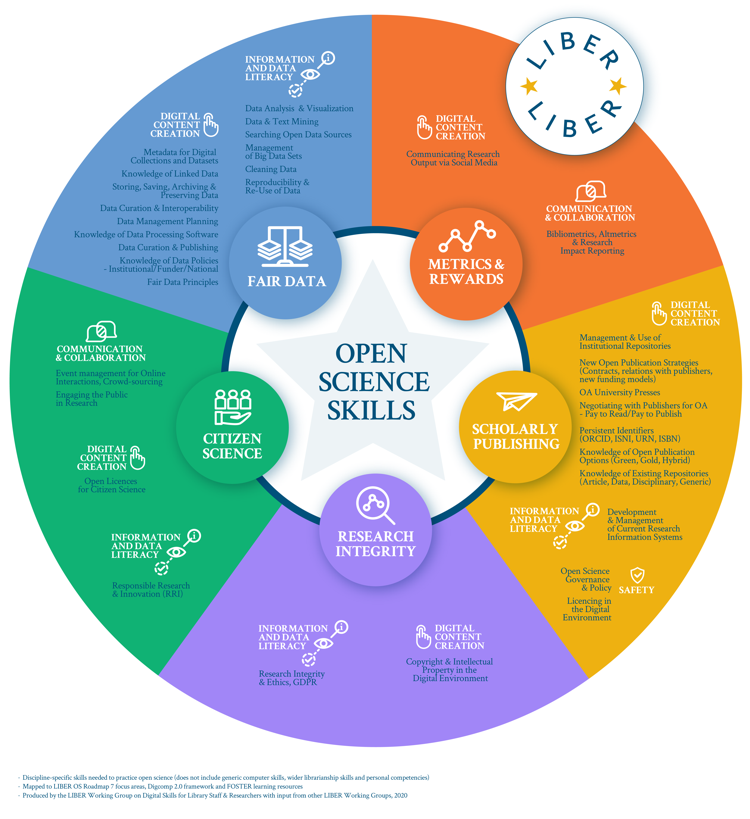
\includegraphics{ethos-of-open/img/image_3_lesson_5_open_science_skills.png}

}

\caption{Open science skills diagram - visit source below to see in
detail}

\end{figure}

\href{https://doi.org/10.5281/zenodo.3702401}{Source} of the visual

\hypertarget{summary-of-the-module}{%
\section{Summary of the module}\label{summary-of-the-module}}

This module provided a broad overview of the \emph{ethos} of responsible
Open Science, the imperative for scientific and societal challenges and
opportunities in the 21st century, and an introduction to how you and
your research team can begin to follow leading practices to enable open
science. Part of the ethos is to help enable these practices within your
team and with your colleagues--that is, you are encouraged and empowered
to share what you have learned and help them learn about, be aware of,
and practice Responsible Open Source.

In a larger context, many of you will be participating in scholarly
efforts, including in peer review, in leadership positions as journals
and societies, in organizing meeting sessions, and more. Enabling
responsible Open Science is a broader cultural shift in scholarly
practices worldwide. In many ways, the recognition, reward and award
systems in science are not fully aligned yet with responsible Open
Science as this cultural shift is ongoing. You are encouraged to
leverage this learning in having conversations to develop this culture
broadly.

Here are the six key guidelines to start practicing and supporting open
science responsibly:

\begin{enumerate}
\def\labelenumi{\arabic{enumi}.}
\tightlist
\item
  Plan for responsible Open Science from the beginning and begin
  discussions in your group, with colleagues, and your librarian.
\item
  Plan for making data and code open and available in leading
  repositories and citing it in publications in the reference section.
  Cite others' data and software that you make use of.
\item
  Learn about and adopt open science tools
\item
  Develop and foster inclusive workgroups, meeting sessions, and
  meetings.
\item
  Learn the routes to make your publications open and what your
  institution supports and funders require; preprints provide an easy
  and robust route
\item
  Support and inform your colleagues.
\end{enumerate}

\hypertarget{questionsreflection-4}{%
\section{Questions/Reflection:}\label{questionsreflection-4}}

\begin{itemize}
\tightlist
\item
  How can a researcher publish in an open access journal ?
\item
  Predatory journals are very harmful and some early career researchers
  may not be even familiar with these journals. Describe why they should
  be not included in responsible Open Science. Also discuss what are the
  possible ways to restrict and control these journals?
\item
  Why are licenses an integral part of Open Science practice ?
\item
  Can you briefly describe the differences between licence types? When
  conflicts arise among co-authors about which types of licenses they
  should choose, how do you discuss and resolve the issue using your
  knowledge learned from this lesson?
\item
  What are two types of permanent identifiers, and why are they useful?
\end{itemize}

\hypertarget{opensciency-ethos-of-open-science-authors}{%
\chapter{OpenSciency Ethos of Open Science:
Authors}\label{opensciency-ethos-of-open-science-authors}}

\textbf{Tomoko Tomo Bell}

University of Guam

\url{https://orcid.org/0000-0003-4606-6307}

\url{https://github.com/TomoCoral}

\textbf{Ismael Kherroubi Garcia}

Open Life Science and Royal Society of Arts, Manufactures and Commerce

\url{https://orcid.org/0000-0002-6850-8375}

\url{https://github.com/Ismael-KG}

\url{https://twitter.com/hermeneuticist}

\textbf{Amber Osma}

DOAJ

\url{https://orcid.org/0000-0003-1198-7843}

\url{https://github.com/aosman12}

\url{https://twitter.com/amb3r12}

\textbf{Miguel Silan}

Annecy Behavioral Science Lab; Université Lumière Lyon 2

\url{https://orcid.org/0000-0002-7480-3661}

\url{https://github.com/miguelsilan}

\url{https://twitter.com/MetaMethodsPH}

\textbf{Yo Yehudi}

Open Life Science

\url{https://orcid.org/0000-0003-2705-1724}

\url{https://github.com/yochannah}

\url{https://twitter.com/yoyehudi}

\textbf{Shamsuddeen Muhammad}

Bayero University, Kano

\url{https://orcid.org/0000-0001-7708-0799}

\url{https://github.com/shmuhammad2004}

\url{https://twitter.com/shmuhammadd}

\part{Open Software}

Have you ever marveled at mesmerizing scientific visualizations and
wondered how they were generated and whether you can recreate them or
even maybe tweak them to produce new results? These types of images have
been created by researchers using \textbf{research software}. These
software products and sometimes their \textbf{source codes} are freely
available to the public. Reproducing such results and using them to
advance the knowledge produced by these types of research software
products are among the pillars of open science. For example, Figure 1,
is generated using \href{https://e3sm.org/}{E3SM}, an Earth System
model, the source code of which is available on
\href{https://github.com/E3SM-Project/E3SM}{GitHub}.

\begin{longtable}[]{@{}
  >{\raggedright\arraybackslash}p{(\columnwidth - 0\tabcolsep) * \real{1.0000}}@{}}
\toprule()
\begin{minipage}[b]{\linewidth}\raggedright
\includegraphics{https://i.imgur.com/zIdfW3i.jpg}
\end{minipage} \\
\midrule()
\endhead
Figure 1. Global E3SM simulation showing eddy activity, credits M.
Petersen, P. Wolfram and T. Ringler \\
\bottomrule()
\end{longtable}

Now, let's say that you are intrigued by the idea of recreating Figure 1
and tweaking the E3SM's source code. We should start with obtaining the
source code. Someone might ask since this project already has a fancy
website why is the source code on GitHub? Let's assume that we
successfully got the source code and want to start recreating the
figure. Naturally, the next question is how do we install it since there
is no executable file in the source code? Maybe you are used to
installing software packages using
\href{https://en.wikipedia.org/wiki/Wizard_(software)}{installation
wizards}, or maybe you are comfortable working from
\href{https://en.wikipedia.org/wiki/Command-line_interface}{command
line}. Which one is possible or preferable for installing this software?
The next step after installation is running the software and visualizing
the results. So, the question is, for generating the desired outputs,
how do we configure the software, what are the required input data, and
how do we get them? Let's take it a step further and say that you have
some brilliant new ideas and want to implement in the source code,
analyze the outputs, publish the results, and make your code publicly
available. Therefore, the questions become: How do we facilitate
navigating this seemingly complicated source code? After making
modifications, are we allowed to share and republish the modified source
code, and if so, how do go about it? How do we ensure that the
republished code is findable and other researchers can reuse and build
upon it?

The purpose of this module is to answer these questions, provide
guidance for streamlining the workflow and ensuring that we give/get
proper credits, and last but not least, draw your attention to and
promote the importance of contributing and giving back to the Open
Science community.

\hypertarget{open-software-in-the-context-of-open-science}{%
\chapter{Open software in the context of Open
Science}\label{open-software-in-the-context-of-open-science}}

Learning objective:

\begin{itemize}
\tightlist
\item
  Understanding core principals of Open Software
\item
  Learning Open Software terminologies
\end{itemize}

\hypertarget{introduction-4}{%
\section{Introduction}\label{introduction-4}}

The software that is created through/during research can be an important
research product in and of itself. Open science principles like
reproducibility, reusability, and replicability are especially important
when it comes to research software. Within this module we will use the
terms software and code interchangeably. We use these terms refer to any
product written in a programming language, and can cover anything from a
short script to a full software package with a full graphical interface.

\hypertarget{open-science-principles-how-they-relate-to-softwarecode}{%
\section{Open Science Principles: How they relate to
software/code}\label{open-science-principles-how-they-relate-to-softwarecode}}

Reproducing findings of a published study is imperative for the
scientific community. Therefore, results that are produced by a
scientific software should be \textbf{reproducible}, \emph{i.e.}, users
should be able to obtain \textgreater{} ``consistent results using the
same input data; computational steps, methods, and code; and conditions
of analysis'' \footnote{National Academies of Sciences, Engineering, and
  Medicine; Policy and Global Affairs; Committee on Science,
  Engineering, Medicine, and Public Policy; Board on Research Data and
  Information; Division on Engineering and Physical Sciences; Committee
  on Applied and Theoretical Statistics; Board on Mathematical Sciences
  and Analytics; Division on Earth and Life Studies; Nuclear and
  Radiation Studies Board; Division of Behavioral and Social Sciences
  and Education; Committee on National Statistics; Board on Behavioral,
  Cognitive, and Sensory Sciences; Committee on Reproducibility and
  Replicability in Science. Washington (DC): National Academies Press
  (US); 2019 May 7.}.

If software/code used to make a figure or generate results is not shared
along with the results/figures themselves, then it would take
significant time, effort, and likely funding, for another researcher to
reproduce those same results and determine they were correct.

We all aim to make significant contributions to our field and can do
this by ``standing on the shoulders of giants'' (Isaac Newton). By
sharing the code, trust in the work can increase, and future work can
build on it without duplicating effort. Therefore, it is important for a
research software to be developed in such a way that it can be
understood, modified, built upon, or incorporated into other software.
This is called \textbf{reusability}. \footnote{Chue Hong, Neil P., Katz,
  Daniel S., Barker, Michelle, Lamprecht, Anna-Lena, Martinez, Carlos,
  Psomopoulos, Fotis E., Harrow, Jen, Castro, Leyla Jael, Gruenpeter,
  Morane, Martinez, Paula Andrea, Honeyman, Tom, Struck, Alessandra,
  Lee, Allen, Loewe, Axel, van Werkhoven, Ben, Jones, Catherine, Garijo,
  Daniel, Plomp, Esther, Genova, Francoise, \ldots{} RDA FAIR4RS WG.
  (2022). FAIR Principles for Research Software (FAIR4RS Principles)
  (1.0). \url{https://doi.org/10.15497/RDA00068}}

Another important aspect of scientific studies is
\textbf{replicability}, \emph{i.e.}, studies answering the same
scientific questions - but using independent data and/or methods -
should find consistent results \footnote{National Academies of Sciences,
  Engineering, and Medicine; Policy and Global Affairs; Committee on
  Science, Engineering, Medicine, and Public Policy; Board on Research
  Data and Information; Division on Engineering and Physical Sciences;
  Committee on Applied and Theoretical Statistics; Board on Mathematical
  Sciences and Analytics; Division on Earth and Life Studies; Nuclear
  and Radiation Studies Board; Division of Behavioral and Social
  Sciences and Education; Committee on National Statistics; Board on
  Behavioral, Cognitive, and Sensory Sciences; Committee on
  Reproducibility and Replicability in Science. Washington (DC):
  National Academies Press (US); 2019 May 7.} \footnote{National
  Academies of Sciences, Engineering, and Medicine 2018. Open Source
  Software Policy Options for NASA Earth and Space Sciences. Washington,
  DC: The National Academies Press.
  \url{https://doi.org/10.17226/25217}.}.

\begin{quote}
Many communities already have a strong replication tradition, where
trust in any scientific result is built when multiple codes achieve
results that demonstrate consistent behaviors. By requiring multiple
codes to achieve the same scientific finding, replication reduces the
impact of individual code errors or numerical issues. \footnote{National
  Academies of Sciences, Engineering, and Medicine 2018. Open Source
  Software Policy Options for NASA Earth and Space Sciences. Washington,
  DC: The National Academies Press.
  \url{https://doi.org/10.17226/25217}.}
\end{quote}

\hypertarget{open-software-and-open-as-a-spectrum}{%
\subsection{Open Software and Open as a
Spectrum}\label{open-software-and-open-as-a-spectrum}}

As we've said, sharing code can increase trust and lead to better
science by allowing a more thorough review process. However, the degree
to which a code is shared and when that code is shared can vary. Any
sharing is a step on the spectrum of what we will refer to as
\textbf{open software}, the most open of these equates to what is known
in the computer science and software development industry as
\textbf{open source software}. Open software can be a spectrum that can
be anything from sharing an executable of a code with a description of
how it was used to developing the software in a public repository from
the start of the project. There are also a variety of license choices
that can be made under the umbrella of open software which can allow the
developer/researcher to retain various levels of ownership and rights to
future commercialization.

Now, let's take a step back and give formal definitions for some of the
terms that we just used.

\begin{description}
\tightlist
\item[Source Code]
Source code is a human-readable (vs.~machine-readable) text written in a
specific programming language. The goal of the source code is to set
exact rules and specifications for the computer that can be translated
into the machine's language. \footnote{\href{https://www.ionos.com/digitalguide/websites/web-development/source-code-explained-definition-examples/}{Ionos}}
\item[Open Source Software (OSS)]
An Open Source Software is distributed with its source code without
additional cost that makes it available for use, modification, and
distribution with its original rights and permissions. \footnote{\href{https://www.synopsys.com/glossary/what-is-open-source-software.html}{Synopsys}}
\end{description}

We should note that researchers are not always able to share their
complete code, or software package (\emph{e.g.}, due to national
security concerns, data privacy, institutional policies). Again, open
software doesn't necessarily mean open-source software and sharing to
the level that is allowed by funding agencies, institutions, and
security requirements is still a step in the right direction towards a
world with more open science.

From
\href{https://openscapes.github.io/series/mindset.html\#open-as-a-way-to-work}{Openscapes}:

\begin{quote}
Open is a spectrum -- what you share, who you share it with, or how you
share it. It's not all-or-nothing. What: slides, tweets, blogs, forums,
wikis\ldots{} then also code, data, protocols Who: your self, research
group, project team, institution\ldots then also public How: internal
servers, Dropbox \ldots{} then also Google Drive, GitHub, data repos
\end{quote}

We might also add here:

\textbf{When}: at the start of your project, when it reaches its first
fully usable version, at the end during publication, etc.

Before jumping into the next lessons, let's have a brief overview of the
core principals of open source software in general and, more
importantly, in the context of research software.

\hypertarget{core-principals-of-open-source-software-what-research-software-can-move-towards}{%
\section{Core Principals of Open Source Software: What research software
can move
towards}\label{core-principals-of-open-source-software-what-research-software-can-move-towards}}

In the previous section, we provided a formal definition for open
software and open source software. For better understanding, let's
define what these concepts are juxtaposed against: \textbf{Closed Source
Software}

\begin{description}
\tightlist
\item[Closed Source Software (CSS)]
Closed source software is a proprietary software that its source code is
not distributed to the public. Therefore, only the original authors who
created the code exclusively have rights to legally copy, modify,
update, and edit the source code. Closed software imposes restrictions
on what the end user can do with the application, preventing users from
modifying, sharing, copying, or republishing the source code.
\footnote{\href{https://www.ibm.com/topics/open-source}{IBM}}
\end{description}

The major differences between CSS and OSS products are two-fold:
End-users cannot modify CSS products and although, OSS products might
have some restrictions on redistribution, CSS products usually are more
restrictive on their terms of usage and redistribution. We can think of
OSS as a form of thinking based on intellectual freedom that follows
three core principles: transparency, participation, and collaboration.
\footnote{\href{https://www.ibm.com/topics/open-source}{IBM}}

\begin{description}
\tightlist
\item[Transparency]
Operating in such a way that it is easy for others to see what actions
are performed and implies openness, communication, and accountability.
\footnote{\href{https://en.wikipedia.org/wiki/Branching_(version_control)}{Wiki-Branching
  (version control)}}
\item[Participation]
Actively giving back and contributing to OSS through either committing
time and lending skills, or monetary sponsorship. \footnote{\href{https://opensource.com/principles}{OpenSource}}
\item[Collaboration]
Collective engagement toward making improvements and advancements
through knowledge sharing and creating an inclusive environment.
\footnote{\href{https://opensource.com/principles}{OpenSource}}
\end{description}

The exchange of ideas and software developed by communities has driven
creative, scientific, and technological advancement in nearly every
aspect of our lives. Developers share insights, ideas, and code to
create innovative software solutions both collectively and individually.
Open source software operates with the underlying principles of peer
production and mass collaboration, creating more sustainable software
development for end users. \footnote{\href{https://www.ibm.com/topics/open-source}{IBM}}

Not only users can make any kind of changes to the source code, but they
can repurpose it into other new software and distribute their own
software. However, there are some nuances on redistribution that we will
cover in
\href{https://hackmd.io/@TOPS-OC3-code/rk2U4xz5q/\%2FtDBYARbRTZObZUQuKbFJ6Q}{Lesson
3}.

Open source software is also sometimes conflated with the free software
movement. Usually, ``free software'' is meant to emphasize freedom in
the rights of end-users, but can sometimes be confused as meaning ``free
of cost''. In actuality, neither free software nor open source software
denote anything about cost---both kinds of software can be legally sold
or given away. Free software and open source software share common
values, and the terms are sometimes combined in the popular phrase
``free and open source software'' (FOSS). \footnote{\href{https://www.redhat.com/en/topics/open-source/what-is-open-source-software}{RedHat}}

To support adapting OSS principals (transparency, participation, and
collaboration), several new concepts have been introduced by the open
source community. These are especially useful in the move to open
science and has produced tools and methodologies that can be used to
make research software more open:

\begin{itemize}
\item
  To facilitate sharing and community engagement a central file location
  storage is needed for source codes which is called a \textbf{Code
  Repository}. Some examples of such repositories are
  \href{https://github.com/}{GitHub},
  \href{https://about.gitlab.com/}{GitLab}, and
  \href{https://bitbucket.org/product/}{Bitbucket}. Although, source
  code sharing and community engagement are their most basic
  capabilities, they go much beyond that and provide a wide range of
  tools for code \emph{testing} and \emph{version control}. Code testing
  in general refers to the process of evaluating and verifying that a
  software product does what it is supposed to do. The benefits of
  testing include preventing bugs, reducing development costs, and
  improving performance \footnote{\href{https://www.ibm.com/topics/software-testing}{IBM
    software testing}}. There are various types of tests with different
  objectives that will be covered in more details in \href{link}{Lesson
  5}. Version control is the practice of tracking and managing changes
  to source code over time. It keeps track of every modification to the
  code in a special kind of database. If a mistake is made, developers
  can turn back the clock and compare earlier versions of the code to
  help fix the mistake while minimizing disruption to all team members
  \href{link}{Lesson 5}. \footnote{\href{https://www.atlassian.com/git/tutorials/what-is-version-control}{Atlassian}}
\item
  In addition to sharing the source code, software executables require a
  storage location to facilitate \emph{software packaging} (for
  developers) and installation process (for end-users). These types of
  storage locations are called \textbf{Software Repositories}. These
  repositories are usually programming language dependent, for example,
  \href{https://pypi.org/}{PyPi} and \href{https://docs.conda.io}{Conda}
  for Python-based software, \href{https://cran.r-project.org/}{CRAN}
  for R-based software, and \href{https://juliapackages.com/}{Julia
  Packages} for Julia-based software. However, software packaging cannot
  always be done using automated services such as PyPi due to
  complexities of the source code structure itself (\emph{e.g.},
  intricacies of the software objectives, use of several programming
  languages, etc.) and/or its dependencies (other software packages that
  it depends on). In these situations, \emph{containerization} is a
  viable option. \href{https://www.docker.com/}{Docker} and
  \href{https://apptainer.org/}{Apptainer} are example services for
  containerization.
\end{itemize}

\hypertarget{summary-3}{%
\section{Summary}\label{summary-3}}

Here we introduced the concept of open software, how it relates to the
broader open science principles, and how sharing and openness can be a
spectrum. At the most open end of this spectrum is what the computer
science/software development community refers to as open source
software. The core principles of open source software are introduced as
a paradigm towards which research software can move towards. The tools
and methodologies developed by the open source community are
particularly helpful in opening research software. Next, we'll dive into
the benefits and hurdles associated with having open software.

\hypertarget{the-pros-and-cons-of-open-software}{%
\chapter{The Pros and Cons of Open
Software}\label{the-pros-and-cons-of-open-software}}

Learning objective:

\begin{itemize}
\tightlist
\item
  Benefits of Open Software for developers and users
\item
  Understanding the responsibilities of developers and user for a
  thriving Open Software culture
\end{itemize}

\hypertarget{introduction-5}{%
\section{Introduction}\label{introduction-5}}

This lesson addresses particular benefits of open-software, presenting
how you as a researcher can benefit from it, and also how can it improve
your research, moving yourself and your teams towards Open Science. We
will also address some common challenges - and misconceptions - of
adopting open software, and how to overcome them.

\hypertarget{benefits-of-open-software}{%
\section{Benefits of open software}\label{benefits-of-open-software}}

Open software offers a multitude of advantages to both developers and
users. There are several benefits of open software are highlighted in
this section.

\hypertarget{as-a-developerprovider}{%
\subsection{As a developer/provider}\label{as-a-developerprovider}}

\begin{itemize}
\item
  \textbf{High Visibility}: Publishing open software enables the
  repository to be more reachable and attainable. It can broaden the
  audience from a diverse group and draw more attention to the software
  repository.
\item
  \textbf{Long-term Sustainability}: Subsequently, open software allows
  more people to access the repository and can cultivate more users to
  be involved in its development. It results in the long-term
  sustainability of the software. \footnote{\href{https://helda.helsinki.fi/handle/10138/157663}{Forking:
    the Invisible Hand of Sustainability in Open Source Software}} Since
  it is unlikely to have perfect software, having a larger user base is
  likely to have more collaboration or feature requests that can
  directly contribute to some improvements in the software. ``Given
  enough eyeballs, all bugs are shallow.'' \footnote{\href{http://www.catb.org/~esr/writings/cathedral-bazaar/cathedral-bazaar/}{Linus'
    Law}} Testing out software with a large base of users can easily
  detect the issues in the software, and they can submit bug reports or
  submit proposed fixes directly.
\item
  \textbf{Quality Improvement}: Besides bug fixes, the contributions can
  also be in feature enhancement, such as submitting additional features
  to the software repository or proposing modified codes that increase
  the effectiveness of the software. As a result, open software that
  comes with community support will tend to have continuous improvement,
  unlocking the potential to create new inventions, and produce better
  quality software versions. By ensuring the quality of the open
  software, it can gain users' trust to rely on it rather than
  redeveloping a software, therefore, minimizes the duplication of
  efforts, both within an organization and across organizations, by
  allowing for individual components to be shared.
\item
  \textbf{Future Employability}: As a developer or maintainer of open
  source software, your skills and experience are an important asset to
  improve your chances of getting a job. \footnote{\href{https://link.springer.com/article/10.1007/s10664-018-9660-3}{Categorizing
    the Content of GitHub README Files}} Experience in developing open
  software is a positive portrayal of the abilities as it helps in
  demonstrating technical abilities. In addition, it also demonstrates
  the personality and work ethic in software development. If someone has
  experience working on complex software development and maintenance, it
  can make the profile outstanding, especially to companies that will
  take into account the contributions of the candidate to open software.
  The hiring manager may also view the product or shared code. Hence,
  open source provides visibility into both how a candidate solves
  problems, and how they collaborate in a team.
\end{itemize}

\hypertarget{as-a-user-salem}{%
\subsection[As a user ]{\texorpdfstring{As a user
\footnote{\href{https://www.sciencedirect.com/science/article/pii/S1877050915017172}{Open
  Source Software (OSS) Quality Assurance: A Survey Paper}}}{As a user }}\label{as-a-user-salem}}

\begin{itemize}
\tightlist
\item
  \textbf{Accessibility}: Shared code certainly increases the
  democratization of science, it promotes more diverse and inclusive
  community to use the open software without a cost-prohibitive barrier.
\item
  \textbf{Flexibility}: Open software provides users a certain freedom
  to utilize the software for any purposes as they wish. It also allows
  users to make changes freely on the software and customize it
  according to their needs or even redistribute the software based on
  the license that has been applied.
\item
  \textbf{Knowledge Sharing}: Open software is also a great learning
  opportunity for the community \footnote{\href{https://www.synopsys.com/glossary/what-is-open-source-software.html\#:~:text=Open\%20source\%20fosters\%20ingenuity\%3B\%20programmers,learning\%20opportunities\%20for\%20new\%20programmers.}{Synopsys}},
  it can help to achieve knowledge sharing through the community, which
  in turn, increases motivation for a continued practice.
\end{itemize}

\hypertarget{are-there-any-disadvantages-of-open-software---and-if-so-how-to-mitigate-them}{%
\section{Are there any disadvantages of open software - and if so, how
to mitigate
them?}\label{are-there-any-disadvantages-of-open-software---and-if-so-how-to-mitigate-them}}

Making a software open source and valuable to the community requires
additional efforts and considerations. In this section, we will discuss
responsibilities that come with this decision and provide you with
guidance for maximizing the impacts of your efforts.

\hypertarget{as-a-user}{%
\subsection{As a user}\label{as-a-user}}

\hypertarget{require-a-skill-set}{%
\subsubsection{Require a skill set}\label{require-a-skill-set}}

Open software comes in many forms and shapes. There are open-source
codes that come as packages available in a repository for a programming
language or environment (\emph{e.g.} PyPi for Python, CRAN for R, Conda
for a variety of languages). Others are code that require installation
from scratch. Even for skilled programmers, this setup can incur in
costs (time and financial).

So, if you are familiar with a programming language that offer
repositories which are easy to download from within your environment
(\emph{e.g.}, R), you can start from there, and build up your confidence
and skills.

To compile and generate an executable code from a repository from
scratch, you will need to be able to check for the necessary computation
environment, check and install dependencies, and compile the code.
Programming language might be a barrier, as well as operating within a
command line environment. The good news is that there are many resources
to help you go through these stages. Widely used open software are
usually well documented, with step-by-step instructions, and some even
have a community which can offer support for installation and running
their code. Sometimes, developers share alongside their open-source code
an executable version for your operating system. \emph{E.g.}, the
repository of
\href{https://github.com/nmfs-stock-synthesis/stock-synthesis/releases}{Stock
Synthesis}\footnote{Methot Jr, R. D., \& Wetzel, C. R. (2013). Stock
  synthesis: a biological and statistical framework for fish stock
  assessment and fishery management. Fisheries Research, 142, 86-99.
  \url{https://doi.org/10.1016/j.fishres.2012.10.012}}, a software used
for stock assessment of fisheries populations, offers both the source
code and compiled versions for different operational systems. So these
are good choices for a beginner.

Bear repeating that while learning these skills incur a cost, by doing
so you might not only gain access to a useful research tool, but might
also gain experience and skills that are useful for your career.

\hypertarget{depreciation}{%
\subsubsection{Depreciation}\label{depreciation}}

Technology changes fast, and software - open and closed - becomes
depreciated. If you rely on a certain open-source tool for your work,
you run the risk of it becoming depreciated. It can happen to projects
that are not maintained, or no longer maintained, for a number of
reasons.

If this happens to you code you use, you can offer the developer to be a
contributor to their open-software and update the code yourself. This
will require programming skills, but it is a viable route. You can also
team up with other users for a group effort.

If you are choosing a tool and are not interested to fix depreciation
issues in the future, aim for widely-used community open software, which
are maintained by numerous people and thus, less likely to be
depreciated.

\hypertarget{security-concerns}{%
\subsubsection{Security concerns}\label{security-concerns}}

Open-software can be perceived as to present more vulnerabilities than
proprietary software - when all software can present vulnerabilities.
You should check if your institution has an open software security
policy in place - if so, follow their guidelines to assure compliance
and up-to-date security protocols \footnote{\href{https://www.linuxfoundation.org/}{Linux
  foudnation}}. To minimize security risks, we also encourage you to
download code/software from an authoritative source - such as the
original project repository - rather than a third party site.

However, an important benefit of open source is that you can see exactly
what the code is doing and know what are the dependencies, what is
useful if any of them becomes vulnerable. You don't have the same level
of transparency with a closed-source code. Open source codes also might
have (some or many) eyes on them, which can result in better oversight.
Widely-used open software will have a community of researchers and
developers working on its code, looking closely at inputs, outputs and
computer performance. But always, check with your institution about
their requirements, guidelines and policies regarding open-source
software.

\hypertarget{as-a-developerprovider-1}{%
\subsection{As a developer/provider}\label{as-a-developerprovider-1}}

\hypertarget{open-software-can-require-extra-work}{%
\subsubsection{Open Software can require extra
work}\label{open-software-can-require-extra-work}}

Some extra work might be required to share code that is already written
to improve readability (\emph{e.g.}, comments, variable names,
indentation) and documentation (\emph{e.g.}, README and code of conduct
files) of your work, so others can easily understand it and use it.
However - and we cannot stress this enough - open software is a journey,
not a destination. How much to change and add is totally up to you. The
important part is to publicly share your code.

By writing code that is easily readable by humans, you can make it more
usable even to yourself! It will save you time when you want to re-use
it years later. Moreover, the more upfront effort you put into
developing an accessible code, the more others will be able to use it -
which might lead to more collaborations, better feedback, and career
opportunities.

There is also a time commitment for basic steps of creating
documentation, choosing a license, getting a DOI. Our module gives you
an understanding of these terms, providing you a checklist with clear
steps to sharing your code. We also point you to resources to make this
process smooth and save you time in decision-making.

After sharing your code in a repository, you will have a reliable backup
that won't depend on your own hard drive - and you have many free
options to choose from! Added benefits are that by creating a license,
you are allowing others to use your work on the terms you will choose.
By having a \href{link}{DOI}, your code is a findable (by online search
engines) and \href{http://citeas.org}{citable} reference, and you thus,
you will get credit for your work! You can also learn more about DOIs in
the lesson about \href{link}{Licenses}.

\hypertarget{becoming-a-maintainer}{%
\subsubsection{\texorpdfstring{Becoming a
\href{vocab}{maintainer}}{Becoming a maintainer}}\label{becoming-a-maintainer}}

Maintaining an open software (particularly open-source) long-term can
bring its special sets of challenges - from the time commitment, to the
procurement of funding, to navigating requests from users. Maintaining
your code after sharing it is a personal choice, and you can step out of
this role at any time you chose (more about this in \href{link}{Lesson
5}{]}).

\hypertarget{sustainability}{%
\subsubsection{Sustainability}\label{sustainability}}

Despite the importance of open-software for researchers, support and
incentive for open-software development and maintenance are frequently
inadequate \footnote{ARDC Ltd.~(2022). A National Agenda for Research
  Software. Viewed online at:
  \url{https://doi.org/10.5281/zenodo.6378082}} \footnote{NAA, N. A. of
  A. (2021). Current state assessment \textbar{} naa.gov.au. September,
  1--127.
  \url{https://www.naa.gov.au/information-management/building-interoperability/interoperability-development-phases/current-state-assessment}}
\footnote{Akhmerov, A., Cruz, M., Drost, N., Hof, C. H. J., Knapen, T.,
  Kuzak, M., Martinez-Ortiz, C., Turkyilmaz-van der Velden, Y., \& van
  Werkhoven, B. (2020). Raising the profile of research software:
  Recommendations for funding agencies and research institutions in the
  Netherlands. Zenodo.} \footnote{Katz, D.S., Druskat, S., Haines, R.,
  Jay, C. and Struck, A., 2019. The State of Sustainable Research
  Software: Learning from the Workshop on Sustainable Software for
  Science: Practice and Experiences (WSSSPE5.1). Journal of Open
  Research Software, 7(1), p.11. DOI:
  \url{http://doi.org/10.5334/jors.242}}\footnote{National Academy of
  Sciences (2018). In Open Source Software Policy Options for NASA Earth
  and Space Sciences. \url{https://doi.org/10.17226/25217}} \footnote{Mangul
  S, Mosqueiro T, Abdill RJ, Duong D, Mitchell K, et al.~(2019)
  Challenges and recommendations to improve the installability and
  archival stability of omics computational tools. PLOS Biology 17(6):
  e3000333. \url{https://doi.org/10.1371/journal.pbio.3000333}}. As
reported by the Australian Data Commons (2022):

\begin{quote}
Software is an often invisible part of research, produced quickly within
a funding window, often struggling to be maintained beyond that.
\footnote{ARDC Ltd.~(2022). A National Agenda for Research Software.
  Viewed online at: \url{https://doi.org/10.5281/zenodo.6378082}}
\end{quote}

Contributions to open software within traditional academia don't carry
the same weight as publications - software is often seem as a by-product
of research, and dedicated funding is unusual \footnote{ARDC
  Ltd.~(2022). A National Agenda for Research Software. Viewed online
  at: \url{https://doi.org/10.5281/zenodo.6378082}} \footnote{NAA, N. A.
  of A. (2021). Current state assessment \textbar{} naa.gov.au.
  September, 1--127.
  \url{https://www.naa.gov.au/information-management/building-interoperability/interoperability-development-phases/current-state-assessment}}
\footnote{Akhmerov, A., Cruz, M., Drost, N., Hof, C. H. J., Knapen, T.,
  Kuzak, M., Martinez-Ortiz, C., Turkyilmaz-van der Velden, Y., \& van
  Werkhoven, B. (2020). Raising the profile of research software:
  Recommendations for funding agencies and research institutions in the
  Netherlands. Zenodo.} \footnote{Katz, D.S., Druskat, S., Haines, R.,
  Jay, C. and Struck, A., 2019. The State of Sustainable Research
  Software: Learning from the Workshop on Sustainable Software for
  Science: Practice and Experiences (WSSSPE5.1). Journal of Open
  Research Software, 7(1), p.11. DOI:
  \url{http://doi.org/10.5334/jors.242}} \footnote{National Academy of
  Sciences (2018). In Open Source Software Policy Options for NASA Earth
  and Space Sciences. \url{https://doi.org/10.17226/25217}} \footnote{Mangul
  S, Mosqueiro T, Abdill RJ, Duong D, Mitchell K, et al.~(2019)
  Challenges and recommendations to improve the installability and
  archival stability of omics computational tools. PLOS Biology 17(6):
  e3000333. \url{https://doi.org/10.1371/journal.pbio.3000333}}. As
reflected by reports and analyses from several countries, a shift in
paradigms of funding and career advancement are required, along with an
increase in software literacy, so open-software can be more sustainable.

While this is a larger, structural issue that cannot be easily overcome
by an individual, we have strength in numbers. More researchers in the
open-source community, will result in more visibility of these issues,
both for our institutions and funding entities. As more researchers move
towards an open, collaborative framework of science, it is expected that
more changes will happen to the current paradigm, allowing a fruitful
future for open-software.

\hypertarget{summary-4}{%
\section{Summary}\label{summary-4}}

In this module, you reviewed particular benefits of open software to
improve: 1) visibility of your work, 2) Long-term Sustainability, 3)
Quality of your software, and 4) your career prospectus. You also could
explore how open-software furthers the open-science principles,
increasing 1) accessibility, 2) freedom, and 3) democratization of
science.

Despite its multiple benefits, adopting and creating open-software also
brings challenges. In this module, we addressed some common challenges,
with some tips to overcome - perceived and real - barriers to
open-software.

Lastly, we want to emphasize that adopting open-software (as a user or
as a developer) on your research is a journey. As with the practice of
open-science, there is a spectrum, and you make your own choices of how,
what and when you are able to share, given your personal skill set,
institutional policies, time and funding limitations. The most important
is to take the first steps, and continue this journey together with the
open-source community.

\hypertarget{licensing-ownership-dois}{%
\chapter{Licensing, Ownership \& DOIs}\label{licensing-ownership-dois}}

Learning objective:

\begin{itemize}
\tightlist
\item
  Understanding ethical and legal aspect of giving credits and
  attributions
\item
  Learning about existing open source licenses and Digital Object
  Identifier
\end{itemize}

\begin{quote}
Disclaimer: the contents of this lesson are for educational purposes
only. They do not constitute legal advice and should not be used as
such.
\end{quote}

\hypertarget{introduction-6}{%
\section{Introduction}\label{introduction-6}}

After deepening your understanding of the reasons to use open-software
in the context of open-science, we here address the first considerations
when using an open software tool in your research. First and foremost,
if you are going to be building your own code on prior work you need to
choose a software that is \textbf{open}, \emph{i.e.,} that you are
allowed to use, modify and redistribute. As a developer, you also need
to ensure that you are sharing a product that is open - and thus, usable
- to others. This is presented on the section \href{link}{Licenses}.

Then, we present how you get credit for your work, and how you give
credit to others' work. This is the content of the section
\emph{Attribution and citation}.

At the end of this lesson, you will be able to: \emph{Choose and abide
by appropriate usage and referencing standards of open-software}.

\hypertarget{licenses}{%
\section{Licenses}\label{licenses}}

A software license is a legal document that grants users particular
rights to the use of a certain software. This license can take many
forms, but in many cases they outline contractual obligations (if any
exist) between the company/software developer behind the software and
the end user, what the user can do with the software, who the user can
distribute the software to (if any such distribution rights exist) and
the length of time the user has the right to use the software.

A user cannot (technically and ethically), use a software without a
license! A user can reach out to the developer/owner to ask for
permission, and go ahead \emph{if} the owner/developer furnishes written
permission. But, if you share your software without a license, no one
can use it without your written permission!

\hypertarget{types-of-licenses}{%
\subsection{Types of licenses}\label{types-of-licenses}}

A license can fall under several categories. License types have general
definitions of what can be done with the software. By picking a type of
license, or by understanding what type the license of a software you're
considering using is, you'll be able to navigate the license process
more quickly than reading each license individually and interpreting the
permissions. An overview of types of licenses is given in the table
below\footnote{\href{https://www.techtarget.com/searchcio/definition/software-license\#:~:text=A\%20software\%20license\%20is\%20a,the\%20software\%20without\%20violating\%20copyrights.}{licensetypes}}:

\begin{longtable}[]{@{}
  >{\raggedright\arraybackslash}p{(\columnwidth - 8\tabcolsep) * \real{0.2667}}
  >{\raggedright\arraybackslash}p{(\columnwidth - 8\tabcolsep) * \real{0.2667}}
  >{\raggedright\arraybackslash}p{(\columnwidth - 8\tabcolsep) * \real{0.1000}}
  >{\raggedright\arraybackslash}p{(\columnwidth - 8\tabcolsep) * \real{0.1000}}
  >{\raggedright\arraybackslash}p{(\columnwidth - 8\tabcolsep) * \real{0.2667}}@{}}
\toprule()
\begin{minipage}[b]{\linewidth}\raggedright
Public domain license
\end{minipage} & \begin{minipage}[b]{\linewidth}\raggedright
Lesser general domain license
\end{minipage} & \begin{minipage}[b]{\linewidth}\raggedright
Permissive
\end{minipage} & \begin{minipage}[b]{\linewidth}\raggedright
Copyleft
\end{minipage} & \begin{minipage}[b]{\linewidth}\raggedright
Proprietary
\end{minipage} \\
\midrule()
\endhead
Anyone can use or modify the software. & Can link to open source
libraries and code can be licensed under any license type. & Has some
requirements for distribution and modification. & Licensed code can be
distributed or modified if all the code involved is licensed under the
same license. & Software cannot be copied, modified or distributed \\
\bottomrule()
\end{longtable}

Summary of selected attributes of licenses types \footnote{Morin, A.,
  Urban, J., \& Sliz, P. (2012). A quick guide to software licensing for
  the scientist-programmer. PLoS Computational Biology, 8(7).
  \url{https://doi.org/10.1371/journal.pcbi.1002598}}:
\includegraphics{https://i.imgur.com/usGIw8P.jpg}

Some of the common licenses used in open software are:

\begin{enumerate}
\def\labelenumi{\arabic{enumi}.}
\tightlist
\item
  MIT license
\item
  Apache License 2.0
\item
  Mozilla Public License 2.0
\item
  BSD 3-Clause ``New'' license
\item
  GNU General Public License (GPL)
\item
  Common Development and Distribution License
\end{enumerate}

For more information on different types of licenses please refer to the
(\href{https://opensource.org/licenses/category}{Open Source Initiative
OSI}).

\hypertarget{how-to-choose-a-license}{%
\subsection{How to choose a license}\label{how-to-choose-a-license}}

There are a number of steps that have to be made before choosing a
particular license. Arguably one of the first decisions to be made is
based upon whether you intend to use the code for commercial purposes or
not, or at least foresee it as a possibility in the future. Some
licenses are more favorable for commercial purposes than others, such as
the \emph{General Public License, version 2}.

The next decision that has to be made is relating to the issue of
distribution. When using other software as a dependency, you should
always be wary of their licenses. Some licenses enforce certain types of
licenses upon redistribution. The GNU GPL, for instance, is incompatible
with proprietary licenses, because it requires the combined work to be
licensed under the GPL, with no additional restrictions allowed. Having
a part of the work under a proprietary license is such an additional
restriction, so you cannot distribute such a combination (unless the
copyright owner of the GPL code gives special permission). \footnote{\href{https://the-turing-way.netlify.app/reproducible-research/licensing/licensing-compatibility.html}{Turing
  Way Compatibility}}

For licensing open software, it is always good practice to consult with
the \href{https://opensource.org/}{Open Source Initiative (OSI)}
website. They provide a list of approved licenses that guides you
through this process. Remember that a first step is always to consult
with your institution (if applicable). You should ensure that you are
complying with any applicable local laws and any policies set by your
employer and/or funding entity.

\begin{figure}

{\centering \includegraphics{https://i.imgur.com/IzeJix8.jpg}

}

\caption{schematic}

\end{figure}

\hypertarget{additional-resources}{%
\subsection{Additional Resources}\label{additional-resources}}

\begin{itemize}
\tightlist
\item
  \href{https://choosealicense.com}{Choosing a License}
\item
  \href{https://the-turing-way.netlify.app/reproducible-research/licensing.html}{Turing
  Way on licensing}
\end{itemize}

\hypertarget{attribution-and-citation-katzsmithchue}{%
\section[Attribution and citation
{[}\^{}Katz{]}]{\texorpdfstring{Attribution and citation
{[}\^{}Katz{]}\footnote{Smith et al.~(2016). Software Citation
  Principles. PeerJ Comput. Sci., DOI 10.7717/peerj-cs.86}\footnote{Chue
  Hong, Neil P., Katz, Daniel S., Barker, Michelle, Lamprecht,
  Anna-Lena, Martinez, Carlos, Psomopoulos, Fotis E., Harrow, Jen,
  Castro, Leyla Jael, Gruenpeter, Morane, Martinez, Paula Andrea,
  Honeyman, Tom, Struck, Alessandra, Lee, Allen, Loewe, Axel, van
  Werkhoven, Ben, Jones, Catherine, Garijo, Daniel, Plomp, Esther,
  Genova, Francoise, \ldots{} RDA FAIR4RS WG. (2022). FAIR Principles
  for Research Software (FAIR4RS Principles) (1.0).
  \url{https://doi.org/10.15497/RDA00068}}}{Attribution and citation {[}\^{}Katz{]}}}\label{attribution-and-citation-katzsmithchue}}

Both when choosing a license and publishing your software for future
citation, a decision has to be made in relation to the issue of
\emph{attribution}, \emph{i.e.}, crediting a person or group of people
or other entity with a particular action in relation to the software.
This can be thought of as the software/code equivalent to authorship on
an academic paper. It is important to consider this to avoid accusations
of plagiarism or copyright infringement. There is a short discussion in
the final lesson in this module regarding ethical considerations on how
contributions can be considered for authorship/attribution/ownership.

When deciding to cite a software or code that was used in your research
you can start with the question: is this research software? Research
software includes source code files, algorithms, scripts, computational
workflows, and executables that were created during the research process
or for a research purpose. Software components (e.g., operating systems,
libraries, dependencies, packages, scripts, etc.) that are used for
research but were not created during or with a clear research intent
should be not be cited (e.g.~Microsoft Word, Linux, Python --the
language itself; specific packages might be citable in this context).
This differentiation may vary between disciplines. Some examples of
research software that would be cited are
\href{https://e3sm.org/}{E3SM}, \href{https://sciml.ai/}{SciML}, and
\href{https://github.com/nmfs-stock-synthesis/stock-synthesis}{Stock
Synthesis}.

The majority of open source software licenses require some degree of
attribution, and a small minority (such as the 0BSD) do not. The license
will also dictate where the attribution must be displayed - some
licenses will require the user to include attribution in a dedicated
file such as the software license agreement.

\hypertarget{digital-object-identifier-doi}{%
\subsection{Digital Object Identifier
(DOI)}\label{digital-object-identifier-doi}}

By having a persistent identifier, a software version can be cited. A
digital object identifier (DOI) is a persistent identifier or handle
used to uniquely identify various objects. It is provided and
standardized by the International Organization for Standardization
(\href{https://www.iso.org/home.html}{ISO}). In contrast to dynamic web
addresses such as URLs, DOIs are static, \emph{i.e.}, do not change over
the life of a document, and point to the location of the document on the
internet. You can get a DOI for your own software/code by adding it to a
preservation repository.

Just as we publish scientific findings in writing in journals to ensure
its preservation over time, its supplementary material, \emph{e.g.},
source code and produced data, should also be stored in a permanent
location. We call these preservation repositories. Some of these
repositories are general-purpose such are
\href{https://zenodo.org/}{Zenodo} and
\href{https://figshare.com/}{Figshare}, and some are more research
field-oriented such as \href{https://www.hydroshare.org/}{Hydroshare}.

It is important to keep in mind that a DOI refers to a static version of
your code and so, you'll need to get a new DOI for each version you
release and want cited. By using the same repository each time you need
a DOI for a new version, you can be sure that when a user looks for your
DOI they are directed towards the most recent version.

\hypertarget{citing-code-without-a-doi}{%
\subsection{Citing code without a DOI}\label{citing-code-without-a-doi}}

As a user, if you'd like to cite a software that does not have a DOI you
can use \href{https://www.softwareheritage.org/}{Software Heritage} to
create a SWH-ID which is also a citable persistent identifier, but can
be created for codes that are not your own. This should only be done
\emph{after} ensuring a DOI is not available otherwise there can be
multiple identifiers being used for the same piece of software.

\hypertarget{attribution-for-piecessnippets-of-code}{%
\subsection{Attribution for pieces/snippets of
code}\label{attribution-for-piecessnippets-of-code}}

While DOI and SWH-ID allow citations of full pieces of software/code,
there is also the case where a small code snippet or section might be
copied into another code. It is common practice to take a few lines of
code to solve a piece of a problem from websites such as
\href{https://stackexchange.com/}{StackExchange} or
\href{https://coderanch.com/}{Code Ranch}, but there should still be an
attribution if no changes are being made. This can be done effectively
with a comment that includes a link to the webpage from which the code
was taken (most sites have an option to create a shortened shareable
link that is more code friendly).

\hypertarget{publishing-open-software-in-peer-reviewed-journals}{%
\subsection{Publishing open software in peer-reviewed
journals}\label{publishing-open-software-in-peer-reviewed-journals}}

It is also possible to publish open software or a research article
detailing the inner workings of that software in peer review journals. A
general example is the \href{https://joss.theoj.org/}{Journal of Open
Source Software}; there are also more discipline specific journals such
as
\href{https://www.journals.elsevier.com/astronomy-and-computing}{Astronomy
and Computing} and
\href{https://www.sciencedirect.com/journal/environmental-modelling-and-software}{Environmental
Modeling \& Software}. The peer review process for some of these
journals may include a review of the code itself, some may be focused
just on the describing journal article that accompanies it. These
publications will also come with a permanent identifier as is customary
with most journal articles.

\hypertarget{external-requirements}{%
\section{External Requirements}\label{external-requirements}}

There are various legal considerations to keep in mind with regard to
software and code you write. For example, these may be considered
intellectual property, and you may wonder who has ownership over it.
Generally speaking much of this is dependent on your employment and
funding situation at the time you did the work. Your institution may
have claim to part or all of the work product, however it is highly
variable, and your institutional offices should be contacted to
understand this better.

There may also be other institutional, governmental, or other legal
policies that may be dependent on your region. Please make sure you
understand your locality's laws and regulations regarding the sharing of
research software and follow your institution and funding agency's
requirements (if any) on licensing and intellectual property.

\hypertarget{additional-resources-1}{%
\subsection{Additional Resources}\label{additional-resources-1}}

\emph{\href{https://scicodes.net}{Code publication}
}\href{https://geodynamics.org}{Computational Infrastructure for
Geodynamics - example of a preservation repository that provides peer
review} \emph{\href{https://f1000research.com/articles/9-1257/v2}{When
to cite software} }\href{http://citeas.org}{CiteAs: a resource for
finding the correct attribution of a research product}

\hypertarget{summary-5}{%
\section{Summary}\label{summary-5}}

Here, we reviewed that a software license is a legal binding document,
made between the developer and the user of a software, which outlines
how that software can be used and distributed. Open software will carry
licenses that follow the \href{https://opensource.org/licenses}{Open
Software Initiative (OSI)} definitions: allowing the software to ``to be
freely used, modified, and shared.''
\href{https://opensource.org/licenses}{(Open Software Initiative OSI)}

We have presented the major categories of licenses that might fall under
the \emph{open-source} definition, and what considerations to take when
choosing a specific software and/or license for your software,
\emph{i.e.} 1) what is the intended use of this software?, 2) how others
can reuse it? And what are the policies of my institution and local laws
regarding open-software use and dissemination?

We have also learned about proper attribution - how to get credit for
your work (DOI, archival of code, publishing options), and how to cite
others work.

\hypertarget{references}{%
\section{References}\label{references}}

\hypertarget{code-managementquality}{%
\chapter{Code management/Quality}\label{code-managementquality}}

Learning objective:

\begin{itemize}
\tightlist
\item
  Understanding some best practices for publishing Open Software
\item
  Learning the basics of code management
\end{itemize}

\hypertarget{introduction-7}{%
\section{Introduction}\label{introduction-7}}

While we maintain that sharing software at all is a great initial first
step regardless of it's state, the more the code is kept clean,
maintained, and documented, the more others will be able to cite, use,
and contribute to it.

\hypertarget{what-does-it-mean-for-softwarecode-to-be-of-good-quality}{%
\section{What does it mean for software/code to be of good
quality?}\label{what-does-it-mean-for-softwarecode-to-be-of-good-quality}}

There are two perspectives that you can take when engaging with this
lesson: a user of open software, or a developer/provider of open
software. As a user, you will want to make sure that a code or software
project you are considering using in your research/project is quality.
As a developer/provider, you will want to make sure your project is of
high enough quality that others will want to use and engage with it.
When we say ``quality'' code, we are referring to precisely that, a
software/code that a user can be confident in using.

Here we outline some baseline expectations for open software. While
there are definitely good open software projects out there that do not
include all of these items (and, unfortunately, plenty of projects out
there that contain many of these items but still don't function well),
this guide will assist in ensuring the software/code that you
develop/use is quality.

\hypertarget{good-documentation}{%
\subsection{Good documentation}\label{good-documentation}}

Good documentation for code is possibly the most important item on this
list for creating a quality code. This will help a user know what the
software does and how it can be used, but also can be a real time saver
for a developer when going back to look at code they haven't looked at
in a while.

\hypertarget{the-readme-file}{%
\subsubsection{The README file}\label{the-readme-file}}

The first stop for a user when they approach a new project should be the
README file. Aptly named, this file should contain orientation
information that will help a user understand the project's purpose as
well as shows examples of how it can be used, and lists most other
important information the creator deems necessary. Note that there is no
one agreed upon convention for the location of these documentation
pieces, so we encourage exploration of the software you're interested
in. Some information we describe as in a README file may be moved into
its own file in some conventions, e.g.~having installation instructions
in an INSTALL file, but the README is still usually the best place to
start. Keeping that in mind, if you are developing a code/software for
use by others, they will expect a descriptive and useful README, without
one using your code may be a nonstarter for many.

\href{https://github.com/MillionConcepts/lhorizon}{Here is an example of
a README file} from a NASA-funded project that shows many of the
specifics we are going to discuss below including multiple installation
options. As you read the suggested parts of documentation below feel
free to reference this for an example.

Let's dive into the specifics of information you should include/find in
a README file. First, a description of what the software does: it's
purpose, the problem it's solving. You don't need to write a whole
academic paper here, a sentence or two is fine. If you do happen to have
a research paper written on the topic no one would be upset if you link
it here, though do be careful that any linked papers are either (a) not
behind a paywall or (b) if it \emph{is} behind a paywall, that the
important information a user would need to use and understand your
software is reiterated separately within the code documentation.

A compatibility description is also necessary. Sometimes this is wrapped
into the installation instructions and that is acceptable. Here the
operating systems (e.g.~Linux, Windows, macOS -- and their versions)
that the software/code works on with are listed. If the code runs in a
browser which does it work with? There are many tools for testing the
compatibility of code across operating systems and environments, we
won't get into those here as they can be specific to the coding language
you're working in.

If installation instructions are not in their own file, they'll live
inside the README. These should be written with very little prior
knowledge expected of the user. Most people are used to downloading a
software package, double-clicking on the executable, and having a setup
wizard walk them through any required steps. Setups such as this are
achieved through packaging. Packaging bundles all the necessary pieces
for a software to run, usually including dependencies, and distributes
it to the user as one ``package''. Packaging software can make
installation a lot simpler for users and allow it to be installed
consistently that aids in reproducibility. Most open software won't be
packaged to the double-click-with-setup-wizard level and some won't be
packaged at all. They will require a bit more up front work for the
user, but an advanced knowledge of installation practices shouldn't be
assumed. For example, an exact command that can be copied and pasted
into the command line is a lot more helpful than something like ``clone
the repo'' or ``install using git pip''.

Usage examples are another important part of a README document. While
how to run and use the software may be obvious to the developer, many
times this is not the case for the user. Simple/small usage examples are
great for the README file. If there are more complex examples that
require input files or that are interactive for the user and the
programming language you are using supports interactive environments,
such as \href{https://jupyter.org/}{Jupyter} (for R, Python, and Julia),
\href{https://github.com/fonsp/Pluto.jl}{Pluto} (for Julia),
\href{https://quarto.org/}{Quarto} (for R, Python, and Julia), and
\href{https://www.rstudio.com/}{RStudio} (for R), these can be used and
included in a repository and pointed to in the README. If interactive
environments are not an option for the language you are using and your
usage examples are necessarily complex, consider writing a standalone
script and including a pointer to this with instructions on how to use
and run that example script in the README.

If relevant, the README is also one of the places you may find
descriptions of the outputs of a software/code. Both what kind of
objects these may be in terms of their type (e.g.~string, integer, etc.)
and in their general description (e.g.~a list of names, the amount of
rain the model calculated, etc.).

As the README is the first place a user will look, this is also where
you can find other notes and caveats of using the software. This should
include at least something on the state of the software: is it in active
development (meaning it may have some bugs and may not always work as
expected), consistently maintained (meaning the software is updated when
necessary--like when a dependency is updated or a bug is reported), or
here for posterity purposes only (meaning the
author/developer/researcher will not be working to maintain or improve
this code any further)? How can you contact the developer/researcher
that created this software/code? How can issue/bugs be reported (if at
all)? This would also be a good place to list any known bugs/issues, so
you get repeat requests.

The README is also a great place to acknowledge team members that worked
on the code/project as well as agencies and grant numbers that funded
the work.

\hypertarget{dependencies}{%
\subsubsection{Dependencies}\label{dependencies}}

The dependencies -- the other software on which the software/code relies
-- should be listed somewhere in the documentation, but are not always
in the same place depending on the coding language. For example, in
Python software, it is common to include a file titled something like
\texttt{environment.yml} which will list dependencies and which can be
used to install them quickly and easily. Other conventions may include
listing them in the README file, a README can also be used to point to
an additional file that lists dependencies (such as the
\texttt{environment.yml} or \texttt{requirements.txt})

\hypertarget{license}{%
\subsubsection{License}\label{license}}

A license file should be included with your documentation. This is
expanded upon more in another lesson in this module, but without one,
the code/software is technically and ethically not allowed to be used at
all by anyone other than the author/developer.

\hypertarget{the-contributing.md-file}{%
\subsubsection{\texorpdfstring{The \texttt{CONTRIBUTING.md}
file}{The CONTRIBUTING.md file}}\label{the-contributing.md-file}}

One of the great benefits of open software is that it enables
contributions from the community. The \texttt{CONTRIBUTING.md} and
CODE\_OF\_CONDUCT files in software can be referenced for information on
how to do this. This is expanded upon more in a later lesson.

\hypertarget{documentation-checklist}{%
\subsubsection{Documentation Checklist}\label{documentation-checklist}}

{[} {]} Description of the software and the problem it solves

{[} {]} Compatibility description

{[} {]} Dependencies

{[} {]} Installation instructions

{[} {]} Usage examples (perhaps including an interactive notebook)

{[} {]} Development status of the software (under development, actively
maintained, etc.)

{[} {]} Contact information

{[} {]} How to report issues/bugs (and a list of any known
issues/limitations)

{[} {]} Acknowledgments of team and funding

{[} {]} License

{[} {]} Contribution guidelines

{[} {]} Code of conduct

Additionally, a GitHub template from NOAA for open software
documentation can be found
\href{https://github.com/NOAA-OWP/owp-open-source-project-template}{here}.

\hypertarget{cleanreadable-code}{%
\subsection{Clean/readable code}\label{cleanreadable-code}}

Code for software is very rarely written only for one individual. Code
typically has to be read and evaluated by others. In private companies,
this is usually because software is written by a group of programmers
and so it is important that programmers are able to read and understand
the code, both in order to improve it and to ``debug'' or fix it. Open
software also operates similarly: there may be many programmers working
and contributing to a particular project from different backgrounds and
walks of life. With different programmers with different backgrounds
collaborating together, it's important that code is transparent and can
be easily understood by others. This is sometimes referred to as ``clean
code''.

Clean code is code that is easily understood by others. Clean code has a
number of advantages. One advantage is that it is easier to spot if or
whether something is wrong with the code (known as ``debugging'').
Another advantage is that code that is ``clean'' is more likely to be
shared than code that is not. This is fundamental to open software,
which aims to be reproduced as widely as possible. There are a number of
principles that should be adhered to when using clean code.

\hypertarget{code-comments}{%
\subsubsection{Code Comments}\label{code-comments}}

Arguably one of the most important is that code should be commented.
Comments are annotations that help other programmers reading to
understand what is going on. In many languages, they are designated by
the sign \texttt{//} or \texttt{\#} or \texttt{/*\ */}. As a rule, more
comments are better than less but this should be prefaced with the
warning that comments should not explain the obvious. For example, in
the language JavaScript, the following would be an inappropriate comment

\texttt{var\ a\ =\ 5;\ //I\textquotesingle{}m\ assigning\ the\ value\ of\ 5\ to\ the\ variable\ a.}

It is inappropriate because the code is self-explanatory.

\hypertarget{descriptive-naming}{%
\subsubsection{Descriptive naming}\label{descriptive-naming}}

Another point to bear in mind when it comes to clean code is that
variables, functions, and similar entities should be given descriptive
names as opposed to vague names. These are names that, when another
programmer reads them, instantly gives an idea of what the variable or
function is. For example, the variable name \texttt{colourOfCat} is a
good name because it describes what it intends to do, which is to
encompass the color of a cat. As a rule, the more descriptive a name for
a variable, function, etc., is the better. Names for variables,
functions, etc. should avoid using words that are likely to be keywords
- names with reserved meanings in many languages - such as ``while'',
``for'', ``override'' and so on. Needless to say, names for variables,
functions, etc. should similarly avoid giving offense and clean code
should consider the sensitivities of those from different backgrounds.

It's frequently the case that code may point to external files; where
possible, a programmer should ensure that the external file has a
descriptive filename. In addition, clean code should also conform to
programming conventions. For example, it's common in many programming
languages to use camel case to describe variables, such as
\texttt{colourForCat} rather than \texttt{COLOURFORCAT}, but one would
do well to ascertain what a convention may be for a particular language.

\hypertarget{whitespace-and-indentation}{%
\subsubsection{Whitespace and
indentation}\label{whitespace-and-indentation}}

Lastly, clean code should contain sufficient spaces between lines of
code (also known as whitespace) and sufficient indentation so that they
are easily discernible. Sometimes code that does not contain sufficient
lines of code can go through a process known as \emph{beautification} or
\emph{prettifying} that helps them become more readable. Ultimately, a
key test for whether code can be considered ``clean'' is the following:
if you left the code and came back to it 2 years from now, would you be
able to easily understand it?

\hypertarget{summary-6}{%
\section{Summary}\label{summary-6}}

In this lesson we go over two main topics regarding markers of quality
code: (1) good, descriptive documentation and (2) clean, readable code.
As a user, documentation can be the difference between spending hours or
days trying to understand a code and being able to use it right out of
the box. As a developer/researcher, documentation improves the
reproducibility and reusability of your code and lets others know what
to expect both of your code and of you yourself as a maintainer. Next,
we'll discuss maintaining quality code.

\hypertarget{references-1}{%
\section{References}\label{references-1}}

\begin{itemize}
\tightlist
\item
  Lee BD (2018) Ten simple rules for documenting scientific software.
  PLoS Comput Biol 14(12): e1006561.
  \url{https://doi.org/10.1371/journal.pcbi.1006561}
\item
  Anzt H, Bach F, Druskat S et al.~An environment for sustainable
  research software in Germany and beyond: current state, open
  challenges, and call for action {[}version 2; peer review: 2
  approved{]} F1000Research 2021, 9:295
\item
  Martin, R. C. (2008). Clean code: A handbook of agile software
  craftsmanship. Prentice Hall.
\end{itemize}

\hypertarget{maintain-good-code-quality}{%
\chapter{Maintain good code quality}\label{maintain-good-code-quality}}

Learning objective:

\begin{itemize}
\tightlist
\item
  Understanding basics of Version Control
\item
  Learning the basics of testing in code development
\item
  Understanding the responsibilities of Open Software developers
\end{itemize}

\hypertarget{introduction-8}{%
\section{Introduction}\label{introduction-8}}

We've talked about markers of quality software in the prior lesson: good
documentation and clean, readable code. The reality is that for most
software, this is a journey, and it is going to continue to change and
develop over some period of time. Here, we discuss version control,
testing, and responsibilities after sharing. These topics are centered
around the evolution of your code and ensuring the work you've done to
make quality open software is able to endure.

\hypertarget{version-control}{%
\section{Version control}\label{version-control}}

Open source codes can change overtime. This brings several challenges to
researchers developing and using an ever-changing software. We covered
the importance of reproducibility for open-software - and open-science
as a whole. Now, how can we achieve reproducibility with a changing code
source? That is done by keeping track of changes to our source code,
using version control.

Version control can be done with tools and systems designed to manage
changes not only to source code, but also to documents, websites, and
datasets. \href{docs.google.com}{Google Docs}, for instance, has its own
complex version control. This allows you and your collaborators to have
access not only to the most updated google document you all are working
on, but to the complete history of changes. So, if something goes wrong
in a document: a child includes a thousand smiley faces in the text, a
cat walks on the keyboard and deletes an entire section - you can just
revert to the earlier, error-free version.

This is the same for coding. For instance, you - the developer - receive
a notification from a user that your code has a bug. You know that this
bug was not present in the last version, so you can easily work through
your history to look what recent changes might have caused a specific
error, narrowing down your debugging work to specific parts of the code.
So, version control allows a group of developers/users to know exactly
what version of the code they are using, what changes were made and when
- facilitating reproducibility. Version control also fosters
collaboration, making it easier for people to work together at the same
time and to merge changes from different users.

There are several version control systems (VCS) available. We won't get
into detail here, but some of the most popular open-source systems
include \href{link}{git}, \href{link}{SVN}, and \href{link}{Mercurial}.
It is important to note that while some repositories have already a
built-in version control, repositories and version control systems are
different - \emph{e.g.}, \emph{git} is the \emph{version control
system}, while \href{https://github.com}{Github} is a \emph{hosting
service} for \textbf{git} repositories.

In \href{link}{lesson 6}, we revisit version control, giving some
concrete examples of how you can use it to contribute for new or
existing open-source code.

\hypertarget{testing}{%
\section{Testing}\label{testing}}

In \href{link}{Lesson 1}, we introduced the concept of code testing and
its importance in software development. There are many types of testing
that range from testing the smallest testable parts of a code to
verifying if a code works as whole under different scenarios. Since code
testing in general can be a complicated and technically involved topic,
we will not go into the details of each types of testing and refer you
to external sources for further reading. Instead, we focus on benefits
and difficulties of testing in general, how to measure test coverage,
and what to expect from a ``tested'' code as an end-user.

We recall that reproducibility in research software plays a critical
role. In the context of testing, we can think of reproducibility as a
test objective of which is to reproduce a specific output, \emph{i.e.},
results obtained from a specific version of the code that has been
published in a journal. This test should include all the required inputs
(configuration files, input data, etc.) so users can easily run and get
the same published results.

More broadly, the main objective of code testing is to evaluate if a
code is doing what it is supposed to do. It is important to recognize
that testing a code comprehensively can be very difficult since not only
we should test the code for generating expected outputs but also for
failing when it should. For example, when an unacceptable input is
passed, \emph{e.g.}, wrong type, out of range, edge cases, etc., or when
if implemented the algorithm doesn't converge for the given set of
inputs. Taking into account all these scenarios can be extremely
difficult and in some cases impossible. Therefore, we should manage our
expectations when taking the tests as a measure of code's quality both
as a developer (\emph{e.g.}, realizing that the end-users might apply
the code to scenarios that we don't anticipate) and an end-user
(\emph{e.g.}, realizing that the difficulties associated with testing
and, if possible, evaluate the accuracy of outputs independently).

From a developer perspective, there are also secondary benefits for
testing. Whenever you make a change to a part of your code, for example
to improve its performance, having tests for that portion of the code,
ensures that the modified code does not change the output. Another
scenario could be related to dependencies. For example, research
software often depends on other software, therefore, if those
dependencies release new versions, the tests help us evaluate if those
new versions make any changes to outputs of our code.

On the other hand, as an end-user, using a code that includes tests,
gives us more confidence in the state of the code. Users can check the
status of tests (pass/fail) when the developers make changes, or the
code has been tested for the use-case of our interest.

Now that we have a better understanding of the testing, we can discuss
measuring its effectiveness. One of the ways that we can measure the
testing is through percentage coverage. There are two levels of
coverage: \emph{test coverage} and \emph{code coverage}. \emph{Test
coverage} refers to the coverage of different scenarios that the code
would be used in while \emph{code coverage} is the percentage of lines
of code that tests cover. As we discussed previously, enumerating all
the different scenarios the code could be used in can be very difficult,
thus, it can be difficult to quantify \emph{test coverage} both from a
developer and end-user perspective. However, \emph{code coverage} is
just a simple percentage value: how many lines of code do the tests
activate vs.~not. It is important to note that a high \emph{code
coverage} does not necessarily mean that a code has good \emph{test
coverage} since testing different usage scenarios can not directly be
translated to lines of code.

\hypertarget{additional-resource}{%
\subsection{Additional Resource}\label{additional-resource}}

\begin{itemize}
\tightlist
\item
  \href{https://www.ibm.com/topics/software-testing}{IBM on Testing}
\item
  \href{https://www.softwaretestinghelp.com/types-of-software-testing/}{Software
  Testing}
\item
  Martin, R. C. (2008). Clean code: A handbook of agile software
  craftsmanship. Prentice Hall.
\end{itemize}

\hypertarget{responsibilities-after-sharing}{%
\section{Responsibilities after
Sharing}\label{responsibilities-after-sharing}}

After sharing software, there are certain steps that need to be taken in
regard to maintenance of that code/software.

First, you should know it is not a requirement for you to be a permanent
maintainer forever, but it is your responsibility to let users know if
you do or don't intend to maintain the software/code. You can do this in
your documentation where you discuss the development status of the
project. This helps a user know if it will continue to be supported in
the future, and make choices about if they should base ongoing work off
your project. You don't want someone to spend a huge amount of time
using your work as a dependency and then have their project become
unusable in the future.

The reality is that a developer/researcher may not have the time or
continued funding to keep up with a project. In this case, perhaps
consider handing ownership of the software to another
researcher/developer, involved user, or entity invested in its continued
use. You can either approach potential parties you think may be
interested in this; or you can make your license permissive enough to
allow others to create their own copies and continue your work (see more
on choosing a license in this module). Depending on the license you
choose, the use of your project, and if you have significant interest,
you may be able to commercialize your software/code to provide funding
for continued maintenance and feature requests. There is also the
potential to apply for continued funding from agencies both governmental
and private if your open software is widely used. If you're a user of a
software that is no longer maintained, consider contacting the
owner/developer and volunteering either as a maintainer, or to take over
ownership of the project (you'll be more likely to get a positive
response if you leave that choice up to the current owner).

If you receive requests for features and fixes, and you have indicated
you intend to maintain the code, these should be responded to. Either
tell the users that (a) you intend to perform their requested action or
(b) you think that's out of scope of your project. Additionally, you can
invite the requester to (a) contribute to the project and add that
feature/fix themselves (which you can then approve and add into your
project) or (b) fork (make a copy of) the project and create the
feature/fix, notifying that you will not merge changes into your
(main/original) copy.

\hypertarget{summary-7}{%
\section{Summary}\label{summary-7}}

Here we discuss how version control and testing can both be used to
increase the reproducibility and trust a user can place in open
software. These are tools that can be used whether your software is
shared or not. We go over what responsibilities a developer/researcher
has after sharing their code: namely to inform your potential users if
you will be maintaining the software and if so, respond to requests for
feature additions and bug fixes. We discuss options for allowing your
code to undergo continued development even if you don't have
time/motivation/funding to continue iteration and encourage users of
code that is no longer maintained to explore these options themselves by
reaching out to the original developers. Furthermore, we discuss how
users can become involved in existing projects in our next lesson.

\hypertarget{contributing-to-existing-open-software}{%
\chapter{Contributing to existing open
software}\label{contributing-to-existing-open-software}}

Learning objective:

\begin{itemize}
\tightlist
\item
  Understanding the importance of contributing to Open Software
\item
  Learning different ways of contributing to open source projects
\item
  Learning best practices for useful contributions to open source
  project
\item
  Learning about ethical aspect of contributions
\end{itemize}

\hypertarget{introduction-9}{%
\section{Introduction}\label{introduction-9}}

In
\href{https://hackmd.io/@TOPS-OC3-code/rk2U4xz5q/\%2FcZYalfBRSCyBTeVtsbfNng}{previous
lesson}, we have discussed the importance of using version control and
testing to maintain good quality of code. Community contributions are
the primary driving force behind open software initiatives. Open
software contribution not only benefits the contributor, but also help
to maintain the software's long-term viability. In this lesson, we will
cover the various types of contributions that can be made, which are not
limited to coding contributions; non-coders can also make significant
contributions to open source software. In addition, we will cover how to
use version control in open-source project contributions; some good
contribution practices will be discussed in this lesson as well.

\hypertarget{benefits-of-contributing-to-an-open-software}{%
\subsection{Benefits of contributing to an open
software}\label{benefits-of-contributing-to-an-open-software}}

Contributing to open software provides many valuable advantages and
opens doors to a number of highly lucrative and rewarding opportunities,
and there are not too many other industries that can boast the massive
number of global contributions like the open-source community can.

A first advantage of contributing to open software is that it will
require you to write clean, documented, structured code. In combination
with the feedback you will obtain from leading developers in the field,
this can help to improve your coding and communication skills.

Secondly, contributions that you have made to open software constitute a
documented and publicly available record of your work (git commits, for
example, get indexed within google search). This allows you to reference
to your contributions as part of a software portfolio or resume,
providing a direct evidence of your work and skills.

Finally, contribution to software by members of the community creates a
unique constellation in which the contributors to the software are also
its main users. Often, contributions to open software stem from users
who wish to improve or change the software for their own use and adapt
the software problem constellations in the software's field of use. This
direct feedback loop between user and developer allows for a fast
development cycle and makes open software more flexible to changes in
needs and requirements than software products that are maintained by a
company.

\hypertarget{types-of-contribution-to-an-open-software-opensource}{%
\subsection[Types of contribution to an open software
]{\texorpdfstring{Types of contribution to an open software
\footnote{{[}opensource
  (https://opensource.com/life/16/1/8-ways-contribute-open-source-without-writing-code)}}{Types of contribution to an open software }}\label{types-of-contribution-to-an-open-software-opensource}}

There are several types of contributing to open software. Not all of
them require writing actual code.

\textbf{Add new features.} The most obvious case for contributing to
open software is enhancing its usability by adding new features. Make
sure to open a new issue first.

\textbf{Fix bugs/issues.} Alternatively, you can reply to an already
opened issue by fixing it. Make sure to reference the issue when
creating a pull request/ request for reviewing your fix.

\textbf{Report issues/ suggestions about improving code.} Reporting an
issue is a valuable contribution even if you don't know how to fix it.
For example, you might be using a different browser in which the
software has not been tested yet, have discovered a particularly
uninformative error message, be colorblind or be otherwise able to feed
a valuable user experience back to the developers that can help to
improve the overall usability of the software.

\textbf{Improving and contributing to documentation.} Contributing to
documentation constitutes a great starting point to contributing to open
source software and is often overlooked in its importance. Writing
documentations allows you to familiarize yourself with the use of the
software, while helping to teach others.

\textbf{Create tutorials, use cases or visuals.} Another way to
contribute is to make your experience and use of the software publicly
available. For example, you could create a tutorial based on your use of
the software, summarize a use case or provide a summary of your use in a
graphic. This part of contribution is particularly appealing as it does
not create much extra work to just publish what you have used the
software for.

\textbf{Improve layout, automatization, structure of code.} Apart from
creating new code, a good way to contribute to open source software can
also be to improve, restructure or automatize existing code. This is
called \emph{refactoring} and helps to make the software project more
effective and stable.

\textbf{Organize/attend a meetup/community building.} Another way to
contribute to open source software is via community building. Many
software products and toolboxes have a lively community of users that
meet on a regular basis in person and online to discuss and improve the
software and its use. Participating or even organizing such a meetup can
be a good way to improve your knowledge of the software, get to know its
community and contribute to open source projects

\textbf{Code review.} Pull requests or other requests to integrate new
contributions into the main code base usually require a review of the
contribution by at least one other user. In the git version control
system, code review entails writing a short summary about the quality of
the code, making suggestions about improvements and then approve or
reject the request.

\hypertarget{how-to-contribute-freecodecamp}{%
\subsection[How to contribute? ]{\texorpdfstring{How to contribute?
\footnote{\href{https://www.freecodecamp.org/news/how-to-contribute-to-open-source-projects-beginners-guide/}{freecodecamp}}}{How to contribute? }}\label{how-to-contribute-freecodecamp}}

Before you contribute to an open source project, there are several
resources that you can check in order to get a feel for the community,
the general environment the software lives in and the contribution and
maintenance process. Below some examples of essential files \footnote{\href{https://link.springer.com/article/10.1007/s10664-018-9660-3}{Categorizing
  the Content of GitHub README Files}} that you might find in a
repository and that might be worth looking at.

\begin{itemize}
\tightlist
\item
  The \textbf{\texttt{README.md}} file gives first information/summary
  about the project. Here you might also find installation instructions,
  software and operating system requirements or a reference to published
  papers on the software.
\item
  The \textbf{\texttt{CONTRIBUTING.md}} file gives information about how
  to contribute to the project. It explains in more detail how the
  contribution process works and what type of contributions are needed.
  While not every project has a \texttt{CONTRIBUTING.md} file, the
  existence of one is a clear indicator that contributions are
  welcomed.\\
\item
  The \textbf{LICENSE} file contains the legal aspects and boundaries of
  contributions. It specifies in which ways the code can be altered and
  how to proceed with altered code. While alterations to code just for
  your private use are usually always possible, the \textbf{license}
  file comes into play in case you intend to publish or commercialize
  and alteration to the software.
\item
  The \textbf{CODE\_OF\_CONDUCT} file: The code of conduct sets ground
  rules for participants' behavior associated and helps to facilitate a
  friendly, welcoming environment. While not every project has a
  CODE\_OF\_CONDUCT file, its presence signals that this is a welcoming
  project to contribute to.
\end{itemize}

\hypertarget{contributing-via-a-version-control-system}{%
\subsubsection{Contributing via a version control
system}\label{contributing-via-a-version-control-system}}

\textbf{Congratulations!} You have decided to contribute to an open
source repository. However, to protect the code in the original
repository, you usually don't have rights to commit directly into that
repository.

Hence, as a user, the next step on your way to a contribution is to
create a \textbf{fork} (a copy of the original repository into your own
account). In contrast to the original repository, you will be
\emph{owner} of the fork, and thus you will have writing rights.

You can also \textbf{clone} this fork onto your local machine. Then
there will be three copies of the repository: The original
\textbf{upstream} repository, the fork in your (online) account, called
\textbf{origin} in git, and the local clone.

Alternatively, as a developer, you can also create a new git repository
from scratch (use \texttt{git\ init} here). This will make you the owner
of the repository and give you writing rights directly.

You can now make changes to your local clone, your local initiated
repository or to your online repository, each of them also being called
your respective \texttt{working\ directory}. Changes to the working
directory will be tracked in a \texttt{staging\ area}, from which you
can and commit them using the command \texttt{git\ commit\ -m\ message}.
If you committed to you local clone or initiated local repository, you
need to push them to the origin repository (your online fork) first, if
you want to make use of them online.

From there, you can create a \textbf{pull request} to an upstream
repository. The owner of upstream repository will then review your
changes and approve them or request changes.

\hypertarget{simple-version-control-workflow}{%
\subsubsection{Simple version control
workflow}\label{simple-version-control-workflow}}

We have again summarized those steps in a checklist for you. We present
here a simple definition of the workflow with common terms you will
encounter, and offer some suggestions for a more in-depth lesson.
\href{https://swcarpentry.github.io/git-novice/}{Software Carpentry} can
be a great place to start!

{[} {]} \textbf{Create Repository}

\begin{itemize}
\tightlist
\item
  Developer: creates a new repository from scratch. Our tip: just go for
  it. You can create your repository with one file, or an entire
  existing open software.
\item
  User: will create a copy (\emph{clone} or \emph{fork}) of an existing
  repository.
\end{itemize}

{[} {]} \textbf{Make changes}

\begin{itemize}
\tightlist
\item
  You can make any changes you want to your copy, but no one will see
  your changes until you \emph{commit} (\emph{i.e.}, submit them).
\end{itemize}

{[} {]} \textbf{Publish your changes}

\begin{itemize}
\tightlist
\item
  If you are like your changes and additions, \emph{commit}. This will
  update your local repository.
\item
  So far, only your local repository has changed. To update your remote
  repository, \emph{push} your modifications.
\end{itemize}

{[} {]} \textbf{Get changes from others}

\begin{itemize}
\tightlist
\item
  While you were working on your copy, other users might have changed
  the remote repository. To keep your local repository updated, you need
  to retrieve, or \emph{pull} the latest changes.
\end{itemize}

{[} {]} \textbf{Keep track of changes}

\begin{itemize}
\tightlist
\item
  To check what is different in your copy since the last commit, you can
  check the \emph{status} of your repository.
\end{itemize}

\begin{figure}

{\centering \includegraphics{https://i.imgur.com/ZQaFMiH.png}

}

\caption{remote}

\end{figure}

As a last note, version control is a good practice for coding, so use it
even if you are not sharing it immediately. You can use version control
with your codes privately on your computer, or use the private mode on
hosting services (\emph{e.g.}, GitHub and GitLab). And, once you are
ready, you are one step ahead to share your code.

\hypertarget{further-resources}{%
\paragraph{Further Resources}\label{further-resources}}

\begin{itemize}
\tightlist
\item
  \href{https://swcarpentry.github.io/git-novice/}{Software Carpentry
  Version Control with Git}
\item
  \href{https://the-turing-way.netlify.app/reproducible-research/vcs.html}{The
  Turing Way, Version Control}
\item
  \href{https://fair-software.eu/recommendations/repository}{FAIR Use a
  publicly accessible repository with version control}
\end{itemize}

\hypertarget{types-of-commits}{%
\subsubsection{Types of Commits}\label{types-of-commits}}

A sustainable open software usually depends on active contribution from
the community through commits access to the repository. In software
version control, a commit is an operation which sends the latest changes
of the source code to the repository \footnote{\href{https://en.wikipedia.org/wiki/Commit_(version_control)}{Wikipedia
  Commit (version control)}}. In general, commit operation can be
classified into 3 categories \footnote{\href{https://dl.acm.org/doi/10.1145/2597073.2597113}{ACM}}
: Core, External, and Mutant.

\begin{itemize}
\item
  \textbf{Core Commit} refer to any commits that directly associated
  with the main repository. The Core Committer usually refers to the
  individual who has write access to the repository of software, and
  responsible for reviewing pull requests
\item
  \textbf{External Commit} is the contributions that go back into the
  upstream repository through patches or pull requests, and it need
  permission from Core Committer.
\item
  \textbf{Mutant Commit} is a modification to the code-base of a project
  which is not incorporated back into the upstream repository. This
  situation happen due to the changes request rejected by the Core
  Committer or the committer intend to personal use only.
\end{itemize}

\hypertarget{branching-and-merging}{%
\subsubsection{Branching and Merging}\label{branching-and-merging}}

In software version control or software configuration management,
branching is the process of object duplication from the original work
under version control. \footnote{\href{https://en.wikipedia.org/wiki/Branching_(version_control)}{Wiki-Branching
  (version control)}} In this context, the duplicated objects are known
as branch. A branch is a version of the repository that deviate from the
main working project, and it is independent line of the development
process.

Branching allows parallel development works including bug fixes, feature
addition, and safely experiment on the same software while retaining the
original source code. The subsections from the main project allow
development teams working on the branch independently and free to make
any changes without impacting on each other.

Every repository has a default branch, which is the first main branch,
and it sometimes called parent branch or upstream branch, whereas the
child branches are the branches from a parent. We can create many
branches from the existing branch. A branch also acts a pointer to one
of the commits in the repository. The HEAD is a special pointer that
simply points to the latest checked out branch or commit. For example,
the default branch named as \texttt{master}, and this master points to
the most recent commit called \texttt{bug-fix}, remember that pointer is
movable when there is new commit.

Upon completion, the branches can be reassembled to the mainline and
become new version of the software release. The process of integrate
changes into the upstream repository is called merging. If you have no
permission to commit directly into the upstream repository, create a
pull request from the branch into main is necessary. It is a good
practice of software development etiquette by ensure the branch is
stable before merging them into main branch. Once the merged completed,
the local branch can be safely deleted. On the other hand, a branch that
not intended to be merged is known as a fork.

In summary, branching and merging is typical process that allows
development team to work on shared codebase and manage the software
effectively.

\hypertarget{merge-conflicts}{%
\subsubsection{Merge conflicts}\label{merge-conflicts}}

\hypertarget{definition}{%
\paragraph{Definition}\label{definition}}

The merge conflicts occur when the version control systems unable to
automatically resolve the differences in codes between two commits. It
requires manual changes and decision to incorporate in the final merge.

Here is an example to explain the scenario, both developer \emph{A} and
\emph{B} make changes on code file in different branch, they make
changes on the same line of codes. During process of merging these two
branches, it will cause merge conflict as it has competing or ambiguity
changes.

\hypertarget{how-to-resolve}{%
\paragraph{How to resolve}\label{how-to-resolve}}

In order to resolve the merge conflict, we must find out where is the
conflict occur, identify the affected code file and specific lines that
causing error, make necessary correction and then make a new commit
before merging these branches again. Make sure latest changes are made
on the file that we want to keep.

\hypertarget{how-to-avoid}{%
\paragraph{How to avoid}\label{how-to-avoid}}

There are few ways to avoid merge conflict, the simplest way is make
sure changes are made on different lines, or different files, to ensure
not introduce any ambiguity lines. Secondly, make sure the local branch
or the branch that currently working on is updated before make any
changes.

\hypertarget{recommended-practices}{%
\subsection{Recommended Practices}\label{recommended-practices}}

Here are some recommended practices {[}\^{}deepsource{]}\footnote{\href{https://www.perforce.com/blog/vcs/8-version-control-best-practices}{Perforce}}
for version control.

\begin{enumerate}
\def\labelenumi{\arabic{enumi}.}
\item
  \textbf{Adhere to templates when opening an issue}

  It is a good practice for version control to check on the
  documentation in open software repository if the repository consists
  of \textbf{\texttt{CONTRIBUTING.md}} file. This file usually is in the
  root directory which describing how others can contribute to the
  project.
\item
  \textbf{Make clean, single-purpose commits}

  It is better to commit the changes with single purpose instead of
  commit combined changes at single time. For example, we prefer push
  the changes for bug fixing and feature adding in different commits.
\item
  \textbf{Write meaningful commit messages}

  It is always best and easy practice to commit the changes with
  descriptive commit messages. A good commit message gives reviewer a
  clear and insightful description about what has been changed.
\item
  \textbf{Commit early, commit often}

  Other than single-purpose commits, commit early is also one of the
  good practice. Commit the work more often and in small chunk will help
  the repository keep updating and avoid conflicts.
\item
  \textbf{Don't alter published history}

  It is strongly not recommend altering the published history. As some
  version control tools allows to rewrite branch history, but it might
  cause unnecessarily confusing.
\item
  \textbf{Don't commit generated files}

  Only commit the files that have been generated manually is also a good
  practice. The files that can be re-generated usually do not work with
  line-based difference tracking.
\item
  \textbf{Refer to issue when creating a pull request}

  If the intention of your pull request is to fix an issue in the
  software, it is highly recommended using a supported keyword in the
  pull request's description or in a commit message. \footnote{\href{https://docs.github.com/en/issues/tracking-your-work-with-issues/linking-a-pull-request-to-an-issue}{Github
    Docs}} Linking a pull request to an issue is certainly helpful for
  showing the status of fixing is in progress.
\item
  \textbf{Assign reviewers}

  Assign reviewers to validate the commit before merging definitely is a
  good practice in contribution as it help to avoid unnecessary conflict
  and quality assurance.
\end{enumerate}

\hypertarget{naming-etiquette}{%
\subsection{Naming Etiquette}\label{naming-etiquette}}

\textbf{Deprecated terms.} \footnote{\href{https://www.theserverside.com/feature/Why-GitHub-renamed-its-master-branch-to-main\#:~:text=The\%20master\%20branch\%20is\%20no,like\%20any\%20other\%20Git\%20branch.}{theserverside}}
The computer industry's use of the terms \emph{master and slave} caught
everyone's attention in the summer of 2020. Amid the many protests and
the growing social unrest, these harmful and antiquated terms were no
longer considered appropriate.

\emph{``Both Conservancy and the Git project are aware that the initial
branch name, `master,' is offensive to some people, and we empathize
with those hurt by the use of that term,''} said the Software Freedom
Conservancy.

The name master for a new repository is outdated and has been replaced
by \emph{main}.

\textbf{Ambiguous terms} While git is the most common version control
system, terms may vary between git and its alternatives.

\hypertarget{ethical-considerations}{%
\subsection{Ethical considerations}\label{ethical-considerations}}

The ability of anyone from the public to contribute to an open source
software project creates an interesting ethical and legal situation
regarding the software's ownership. It should be clear that
contributions such as fixing a typo in the documentation does not create
the right to claim for (partial) ownership of the software, but the
lines for more substantial contributions tend to blur fast and are often
up for discussion. In general, the answer to when a contribution has
altered a software enough to justify a partial transfer of ownership has
to be determined on a case to case basis. Often, this process requires
considering the license and contributing agreements. For example, while
many repositories state for example in their contributing file that
contributing includes a loss of ownership and rights of the code to the
owner of the main repository, other repositories acknowledge already
minor contributions, for example by assigning rights to the repository
or adding the contributor's name to a an acknowledgment file.

\hypertarget{summary-8}{%
\section{Summary}\label{summary-8}}

To summarize, contributing to open software delivers multiple benefits
to the community while also assisting in the product's maintenance.
Contributing to an open source project can help you enhance your
technical abilities and get a better reputation. If you are a coder, you
may typically contribute by reporting issues, resolving bugs, and
creating new features. Aside from that, you can help by producing
documentation, increasing the repository's visibility, or refactoring
it. Both coders and non-coders have an equal opportunity to contribute
to open source software. We explained how to use the basic version
control workflow, which begins with creating a repository, then making
changes, publishing changes, and pulling modifications if any exist, and
finally keeping track of the changes. In general, commit operations are
classified as Core, External, or Mutant. Branching and merging are both
important steps in version control, and merge conflicts should be
avoided. We also talked about creating a list of best practices to which
you can refer before contributing. Nonetheless, there are some ethical
issues to keep in mind while contributing to open source software.

\hypertarget{opensciency-open-software-authors}{%
\chapter{OpenSciency Open Software:
Authors}\label{opensciency-open-software-authors}}

\textbf{Bayer, Johanna}

University of Melbourne

\url{https://orcid.org/0000-0003-4891-6256}

\url{https://github.com/likeajumprope}

\url{https://twitter.com/likeajumprope}

\textbf{Brown, Sierra}

Million Concepts, LLC

\url{https://orcid.org/0000-0001-6065-5461}

\url{https://github.com/Sierra-MC}

\textbf{Chegini, Taher}

University of Houston

\url{https://orcid.org/0000-0002-5430-6000}

\url{https://github.com/cheginit}

\href{https://twitter.com/_taher_}{https://twitter.com/\emph{taher}}

\textbf{Keat, Yeo}

University of Putra Malaysia

\url{https://orcid.org/0000-0001-6935-3101}

\url{https://github.com/ee2110}

\url{https://twitter.com/EeYeoKeat}

\textbf{Onabajo, Babatunde}

ChurchMapped Limited

\url{https://orcid.org/0000-0001-6118-9255}

\url{https://github.com/BabatundeOnabajo}

\url{https://twitter.com/babatundeonabaj}

\textbf{Powell, James}

\url{https://github.com/CRiddler}

\url{https://twitter.com/dontusethiscode}

\textbf{Riddell, Cameron}

\url{https://github.com/dutc}

\url{https://mobile.twitter.com/riddlemecam}

\textbf{Vaz, Ana}

University of Miami

\url{https://orcid.org/0000-0003-0336-5227}

\url{https://github.com/AnaVaz-NOAA}

\url{https://github.com/anacarolvaz}

\url{https://twitter.com/anacarolvaz}

\part{Open Data}

\textbf{Learning objectives:}\\
- Describe key characteristics of open data\\
- Categorize types of open data

\hypertarget{introduction-10}{%
\section*{Introduction}\label{introduction-10}}
\addcontentsline{toc}{section}{Introduction}

\markright{Introduction}

As mentioned earlier, data is a major part of scientific research, and
why wouldn't it be? It is evident that data permeates many aspects of
our daily life with significant consequences.

For instance, it has become all the more common to see news articles
discussing how data and efforts like
\href{https://www.openstreetmap.us/}{Open Street Map} are critical in
supporting the disaster emergency responses all over the world
\href{https://www.openstreetmap.us/}{1}. This is only an example among
many others demonstrating the value of data, particularly open and
public data, in our daily life and for public good.

Similarly, data shared openly in scientific research brings tremendous
value which is not limited to the scientific community but extends to
communities at large from indigenous communities to urban populations!
Before we look further into this, let's first look at what is data in
scientific fields? What is open data? What are the key characteristics
of open data?

\hypertarget{what-is-data}{%
\subsection*{What is Data?}\label{what-is-data}}
\addcontentsline{toc}{subsection}{What is Data?}

\textbf{Data} is any type of information, recordable or observable
facts. \textbf{Research data} is thus data collected in order to answer
the research questions of a project.

Research data can be numbers, texts, measurements, images, model output,
and more. Research data is collected in different ways, and formats.
Generally speaking it can be grouped in different ways, for example:

\begin{itemize}
\tightlist
\item
  Qualitative data describing information in words
\item
  Quantitative data with defined numerical information, e.g.~from
  measurements
\item
  Grouped versus ungrouped data; grouped data being data that has been
  put into classes for next steps such as interpretation and ungrouped
  data referring to the raw data
  \href{https://keydifferences.com/difference-between-ungrouped-data-and-grouped-data.html}{2}
\item
  Structured versus unstructured data: unstructured data referring to
  data in its raw format, and structured data referring to data
  formatted for storage in files or records such as relational databases
  \href{https://www.datamation.com/big-data/structured-vs-unstructured-data/}{3}
\end{itemize}

In the next section we will introduce the different types of data most
commonly generated/found in research. This will provide an understanding
of how different data should be handled and what considerations to keep
in mind when sharing it openly. More on this can be found in lessons 3
(Responsible Open Data) \& 4 (CARE and FAIR Principles). We will also
highlight one particular type of data (metadata, described below) and
its role in supporting the development of Open Data and Open Science
initiatives.

\hypertarget{primary-raw-data}{%
\subsubsection*{Primary (raw) data}\label{primary-raw-data}}
\addcontentsline{toc}{subsubsection}{Primary (raw) data}

Primary data refers to data that is directly collected or created by
researchers. Examples include surveys, questionnaires, interviews,
physical samples, specimens, output from models, remote sensing data
(spectral/photons), etc. Research questions guide the collection of the
data. Typically, a researcher will formulate a question, develop a
methodology and start collecting the data. Some examples of primary data
include:

\textbf{Responses to Interviews, questionnaires, and surveys.}

Typically, interviews generate data, in the form of recorded audio files,
transcripts, and notes and other observational data. Interviews can
address a broad range of quantitative or qualitative oriented research
questions, and may be used on their own or as part of a mixed methods
approach. In behavioral and social sciences, these data collection
methods are often used to collect self-reported data. A researcher
designs these questions to collect data from participants that are
necessary for the research. In most cases, this type of data can be
openly shared under certain conditions or considerations e.g.~if they
are de-identified, and if the participants consent about the data being
shared, more on that in lesson 2 and 3.

\textbf{Data acquired from recorded measurements}, including remote
sensing data.

In many cases, the raw primary measurements from an instrument are
processed in various ways such that what is typically stored and
reported is based on a variety of calibration, normalization, and even
compression steps that are ideally well defined and described by a
discipline or measurement protocol. For example, satellite captured
imagery is often used in online map services and navigation (e.g.,
Google Maps). These satellite imagery is often captured by various
sensors onboard space-borne satellites (e.g.,
\href{https://eospso.gsfc.nasa.gov}{NASA Earth Observing System}) or
airborne measuring platforms (e.g., uncrewed drones or planes)
{[}\href{https://eospso.gsfc.nasa.gov}{4}{]}. These data often need
careful calibration and correction including the values recorded by the
sensors and the geospatial location of the imagery before it can be used
appropriately for research and application. After the calibration and
corrections, remote sensing imagery are often used to create products
that can help us understand the environment that we live in and useful
for societal benefits (e.g., studying air quality impact on community
health).

\textbf{Data acquired from physical samples and specimens} form the base
of many studies.

Tests and analyses are conducted on these resources, such as biological
specimens, rocks and minerals, soils and sediments, plants and seeds,
water samples, archaeological artifacts, or DNA and human tissue samples
(\href{https://www.rd-alliance.org/groups/physical-samples-and-collections-research-data-ecosystem-ig}{Research
Data Alliance Interest Group on Physical Samples})
{[}\href{https://www.rd-alliance.org/groups/physical-samples-and-collections-research-data-ecosystem-ig}{5}{]}.
While it may be more difficult to share these types of physical
resources, information about the samples and as well as data derived
from using them, can be shared via thorough description, such as in the
case of BioBanks, \href{https://www.igsn.org/}{IGSN} (a persistent
identifier specifically for physical samples), and
\href{https://isamplesorg.github.io/home/}{iSamples}
{[}\href{https://www.igsn.org/}{6}{]}
{[}\href{https://isamplesorg.github.io/home/}{7}{]}. For more
information about how to manage physical samples, check out the 23
Things Physical Samples
{[}\href{https://zenodo.org/record/6818076\#.YtgQhITMK3B}{8}{]}.

\textbf{Data generated from models and simulations.}

Not all primary data are observations collected by people or
instruments. We also build mathematical models either based on physical
laws or empirical relationships to understand a subject or system. The
model can produce a suite of simulations driven by various input
scenarios or initial conditions. For example, Coupled Model
Intercomparison Project
(\href{https://www.wcrp-climate.org/wgcm-cmip}{CMIP}) is an
international project with participation from more than 20 earth system
modeling centers to generate the historical simulation and future
projections of the earth system under different greenhouse gas emission
scenarios {[}\href{https://www.wcrp-climate.org/wgcm-cmip}{9}{]}. The
Open Data generated in the most recent phase of CMIP (CMIP6) allows
researchers to understand the impact of the changing climate to the
ecosystem and our society. The understanding derived from CMIP6 data can
then be used to inform climate policies and adaptation strategies. Model
data are valuable assets because it can provide data that can be hard or
sometimes impossible to collect in real world
{[}\href{https://www.climateurope.eu/a-short-introduction-to-climate-models-cmip-cmip6/}{10}{]}.

\hypertarget{processed-data}{%
\subsubsection*{Processed data}\label{processed-data}}
\addcontentsline{toc}{subsubsection}{Processed data}

Processed data typically refers to data that is created or collected by
someone else and used by others.

Examples include data from literature, academic publications, generated
statistics such as government statistics, transcripts of recordings, and
a variety of streaming environmental and biological data that are
deposited and made available in databases and repositories.

This type of data is oftentimes used for a different purpose than
originally intended, for example, from a previous experiment or from
another research project or a different discipline.

It is very common in the era of digital scientific research to see new
primary datasets created or produced by collecting and repurposing
secondary data and/or mixing them with new primary data. This kind of
research practice is made possible by the promotion of Open Data. Data
sharing provides opportunities for all researchers, even the novice
and/or unfunded, therefore leveling the playing field
{[}\href{https://www.sciencedirect.com/science/article/abs/pii/S0023969001910987?via\%3Dihub}{11}{]}.
More on the benefits of Open Data in lesson 2.

\hypertarget{metadata}{%
\subsubsection*{Metadata}\label{metadata}}
\addcontentsline{toc}{subsubsection}{Metadata}

Metadata is a special type of data that describes other data or objects
(e.g.~samples). It is often used to provide a standard set of
information about a dataset to enable easy use and interpretation of the
data.

It can facilitate assessment of dataset quality, by answering key
questions, such as including key information on:

\begin{itemize}
\tightlist
\item
  How the data was collected (e.g.~which equipment/instruments were
  used)
\item
  Which variables/parameters are included in this dataset
\item
  Who or which organization created or collected the data
\item
  When the data was collected and deposited
\item
  Where to find the data (e.g.~DOI) and how to cite it
\item
  Which geographic region the dataset covers
\item
  Who can use the data and how
\item
  Which version is the dataset
\item
  What is the format of the data
\item
  Whether the dataset follows any community or international standards
  or guidelines
\end{itemize}

In addition, metadata allows cataloging and data discovery specially, if
it follows leading practices allowing them to be indexed by search
engines
(\href{https://the-turing-way.netlify.app/reproducible-research/reproducible-research.html}{The
Turing Way, 2019})
{[}\href{https://the-turing-way.netlify.app/reproducible-research/reproducible-research.html}{12}{]}.
In other words, it enhances searchability and findability of the data by
allowing other machines to read and interpret datasets (see the concept
Findable in lesson 4 - CARE and FAIR principles)

In later lessons, we will describe how to create metadata and where to
find help (e.g.~repositories)

There are different types/categories of metadata addressing different
purposes:

\begin{itemize}
\tightlist
\item
  \textbf{Descriptive metadata} can contain information about the
  context and content of your data; such as, abstract, title, subject
  keywords.
\item
  \textbf{Structural metadata} is used to describe the structure of the
  data (e.g., file format, the dataset hierarchy).
\item
  \textbf{Administrative metadata} explaining the information that is
  used to manage the data (e.g., when and how it was created, which
  software and the version of the software used in data creation).
\end{itemize}

\hypertarget{what-is-open-data}{%
\subsection*{1.2 What is Open Data?}\label{what-is-open-data}}
\addcontentsline{toc}{subsection}{1.2 What is Open Data?}

The term ``Open Data'' is relatively new with the first appearance in
1995 in an
\href{http://www.paristechreview.com/2013/03/29/brief-history-open-data/}{article
in Paris Tech Review} describing the need of sharing Earth and
environmental data because ``our atmosphere, oceans and biosphere form
an integrated whole that transcends borders.''
{[}\href{http://www.paristechreview.com/2013/03/29/brief-history-open-data/}{13}{]}

In this lesson, we are adopting the definition of ``Open Data'' as
defined in the \href{https://opendatahandbook.org/}{Open Data Handbook}
from the \href{https://okfn.org/}{Open Knowledge Foundation}
{[}\href{https://opendatahandbook.org/}{14}{]}
{[}\href{https://okfn.org/}{15}{]}.

\begin{quote}
``Open data is data that can be freely used, re-used and redistributed
by anyone - subject only, at most, to the requirement to attribute and
sharealike.'' Open Data is defined by a set of key attributes, but keep
in mind that not all aspects can or will be present at all times as
there might be some considerations or restrictions to take into account.
This could be partly due to the fact that Open Data does not necessarily
mean Open for ALL, but rather Open for the specific individuals and/or
communities, more on this in lessons 3 (Responsible Open Data) \& 4
(CARE \& FAIR Principles) .
\end{quote}

\hypertarget{availability-and-accessibility}{%
\subsubsection*{Availability and
accessibility}\label{availability-and-accessibility}}
\addcontentsline{toc}{subsubsection}{Availability and accessibility}

Open data is characterized by being available and accessible, meaning
that it is published on a publicly available platform and accessible to
download over the internet allowing others to find it and use it.

Ideally, scientific research outputs including; research data, metadata,
manuscripts, open educational resources, software, hardware and source
code are published and made available in both human and machine
readable.

Generally, Open Data does not require a payment. Nevertheless, in some
cases infrastructure costs might be required which can be covered by
societies, institutes, organizations etc. More on this in lesson 6
(Sharing Open Data).

\hypertarget{reusability}{%
\subsubsection*{Reusability}\label{reusability}}
\addcontentsline{toc}{subsubsection}{Reusability}

For Open Data to be useful, it has to be reusable. Without the capacity
to reuse it, we are creating ``data tombs'' where the data is hosted
(lives) but is of no value to others {[}\href{}{16}{]}.

There are essential factors that need to be addressed in order for the
data to be in good enough shape for others to use it .For instance,
researchers and data reusers are mostly looking for data which is
``comprehensive, easy to obtain, easy to manipulate, and believable''.
For these criteria to be fulfilled the data needs to:

\begin{itemize}
\tightlist
\item
  Sufficiently described with appropriate metadata, which greatly
  affects open data reusability. There is no one size fits all for
  metadata as its collection is guided by your data. More on metadata
  generation in lesson 5 (Planning for Open Data)
\item
  Has appropriate license, copyright and citation information. See
  lesson 6 (Sharing Open Data)
\item
  Has appropriate access information. Learn more in lesson 6 (Sharing
  Open Data)
\item
  Findable in an accredited or trustworthy resource. Learn more in
  lesson 6 (Sharing Open Data)
\item
  Maintained on a regular basis, addressing feedback from different
  levels of users
\item
  Accompanied with history of changes and versioning (see definitions)
  allowing users to point to the exact state of data when they decided
  to use it.
\item
  For processed data it is also important to include details of all
  processing steps. For instance in the case for large data, e.g., it is
  not common practice for raw genomic reads to be preserved. In most
  cases processed genomic data are reported, and archived. Hence, some
  case sensitive data should contain information about processing steps
  (e.g., calibration, normalization) depending on varying instances.
\end{itemize}

\hypertarget{inclusivity}{%
\subsubsection*{Inclusivity}\label{inclusivity}}
\addcontentsline{toc}{subsubsection}{Inclusivity}

Data inclusivity refers to making the data truly open and available for
all independent of nationality, location, race, age, gender, sexual
orientation, religion, income, socio-economic circumstances, career
stage, discipline, language and culture, ability and disability,
political ideology, ethnicity or immigration status or any other
grounds.

Open Data is free from all types of organizational, cultural, political
and/or commercial restrictions. A good example of open data transcend
national boundary is the
\href{https://data.worldbank.org/indicator/SI.POV.DDAY?locations=1W\&start=1981\&end=2015\&view=chart}{world
bank poverty} headcount data, which is anonymously developed from
primary household survey data of different government statistical
agencies and World Bank country departments
{[}\href{https://data.worldbank.org/indicator/SI.POV.DDAY?locations=1W\&start=1981\&end=2015\&view=chart}{17}{]}.

The inclusiveness of open data brings many benefits (Lesson 2 - Benefits
of Open Data). However, there are situations when it is not ethical or
appropriate to share certain data, or there are considerations to
implement additional steps and policies to ensure the proper use of open
data (Lesson 3 - Responsible Open Data).

\hypertarget{summary-9}{%
\section*{Summary}\label{summary-9}}
\addcontentsline{toc}{section}{Summary}

\markright{Summary}

In this lesson, you learned about different types of data, the
definition and key characteristics of open data. You might already have
some great examples about open data that you are interested in learning
more. In the next lesson, you will be exposed to various benefits and
challenges of open data.

\hypertarget{assessment}{%
\section*{Assessment}\label{assessment}}
\addcontentsline{toc}{section}{Assessment}

\markright{Assessment}

\textbf{Self Assessment:} Do you know the difference between different
types of data?

A researcher needs data on trauma for an ongoing project.

\textbf{Scenario 1:} They visit a trauma center and ask questions to
patients in the trauma center. What type of data was collected?

\textbf{Senario 2:} In the trauma center, they are referred to a
database where they can find responses from patients. What type of data
was collected? Footer

\hypertarget{references-2}{%
\section*{References}\label{references-2}}
\addcontentsline{toc}{section}{References}

\markright{References}

\begin{enumerate}
\def\labelenumi{\arabic{enumi}.}
\tightlist
\item
  https://www.openstreetmap.us/
\item
  https://keydifferences.com/difference-between-ungrouped-data-and-grouped-data.html
\item
  https://www.datamation.com/big-data/structured-vs-unstructured-data/
\item
  https://eospso.gsfc.nasa.gov
\item
  https://www.rd-alliance.org/groups/physical-samples-and-collections-research-data-ecosystem-ig
\item
  https://www.igsn.org/
\item
  https://isamplesorg.github.io/home/
\item
  https://zenodo.org/record/6818076\#.YtgQhITMK3B
\item
  https://www.wcrp-climate.org/wgcm-cmip
\item
  https://www.climateurope.eu/a-short-introduction-to-climate-models-cmip-cmip6/
\item
  https://www.sciencedirect.com/science/article/abs/pii/S0023969001910987?via\%3Dihub
\item
  https://the-turing-way.netlify.app/reproducible-research/reproducible-research.html
\item
  https://www.paristechreview.com/2013/03/29/brief-history-open-data/
\item
  https://opendatahandbook.org/
\item
  https://okfn.org/
\item
  https://doi.org/10.1093/bioinformatics/btn464\\
\item
  https://data.worldbank.org/indicator/SI.POV.DDAY?locations=1W\&start=1981\&end=2015\&view=chart
\end{enumerate}

\hypertarget{benefits-of-open-data}{%
\chapter{Benefits of Open Data}\label{benefits-of-open-data}}

\hypertarget{learning-objectives}{%
\section{Learning Objectives}\label{learning-objectives}}

\begin{itemize}
\tightlist
\item
  Communicate the benefits and challenges of Open data and it's effects
  on science
\end{itemize}

\hypertarget{introduction-11}{%
\section{Introduction}\label{introduction-11}}

In this lesson, we'll discuss the benefits of open data and in
particular its direct effect in advancing Open Science. We will also
discuss details of how Open Data can impact the response of science in
global emergencies, and how Open Data facilitates multidisciplinary
work.

\hypertarget{open-data-for-the-greater-good}{%
\section{Open Data for the greater
good}\label{open-data-for-the-greater-good}}

As we mentioned earlier, data plays a significant role in our day-to-day
lives. Open Data, in particular, has played a key role. If you pause and
think about it, you may realize that Open Data is not only common in our
society, but you might have benefited from it and used it yourself.

Here, are some notable examples of Open Data that has positively
impacted society at large:

Each country or territory often provides open access to a variety of
socioeconomic information about the population, community, and business
in its jurisdiction. These data are often called census survey data
which may include the aggregated statistics of gender, race, ethnicity,
education, income, and health data of a community. These data are often
used to understand the composition of a local neighborhood and are
critical to inform decisions on resource allocation to ensure the
quality of life for the community.

The changing climate poses a significant risk to our daily lives and has
been responsible for intensifying drought, increasing flooding, and
devastating fire incidents worldwide. Open data is therefore critical in
providing life-saving information to adapt to the changing climate and
help assess the climate risks of the place where we live. Government
agencies (e.g., National Oceanic Atmospheric Administration in the U.S.,
UK Met Office, European Centre for Medium-Range Weather Forecasts) have
been providing public access to long-term weather and climate
information for decades. A more recent initiative stems from
organizations developing value-added open data products to advise
society on the risk of changing climate. One recent example is the flood
and fire risk in the United States developed by a non-profit
organization First Street Foundation

\hypertarget{open-data-for-better-open-science}{%
\section{Open Data for better Open
Science}\label{open-data-for-better-open-science}}

Scientific discovery and innovation stand to gain a tremendous amount
from Open Data. This impact stems directly from the multiple inputs and
methods developed for investigating problems. Specifically, three core
components of Open Data drive this diverse scientific innovation and
provide enormous societal and scientific benefits:

\hypertarget{validation}{%
\subsection{Validation:}\label{validation}}

Open Data that is easily accessible by other researchers allows for
scrutiny, which helps discover mistakes more quickly and ingrains
confidence that the research was conducted with sound and ethical
principles and methods. Evidence-based progress is important in
providing confidence in the scientific results and is important for the
insights drawn to inform future research.

Data that has been reviewed, maintained and scrutinized by many, as well
as informed by diverse consultation, drives robust and thorough
scientific pursuits.

This validation process is a key component of reproducibility, which is
important in building on prior research. Reproducibility is the
cornerstone of pushing science forward, as it is the very baseline to
check results and expand upon them by introducing new experiments and
questions.

\hypertarget{transparency}{%
\subsection{Transparency:}\label{transparency}}

Building on the idea of validation and scrutinization, transparency
facilitates this process. It allows for early engagement with the data
and ensures the data was collected with sound and ethical principles
(these will be elaborated upon in lessons 3 (Responsible Open Data) \& 4
(The CARE and FAIR principles).

This transparency allows for early intervention if there are unexpected
harms. This is where the idea of multiple perspectives becomes important
again. Collaboration:

Open datasets are made available to all (see section Inclusivity in
lesson 1) - which means new, robust insights are gathered at a faster
pace as mistakes can be caught more easily, expensive data collection
doesn't need to be repeated, and researchers build upon the work of
their peers. For example, the first image of a black hole; Scientists
recently produced the first image of a black hole in our galaxy. This
achievement was only possible through open collaboration and sharing of
telescope data by different observatories distributed across different
parts of the world {[}1{]}.

The data isn't limited to those within a specific field nor exclusive to
those with institutional access. Importantly, this means the data can be
shared with non-traditional academic researchers such as nurses, social
workers, agronomists, journalists and other communities. This allows for
researchers to also derive insights from varying perspectives.

The scope of research can be easily expanded to derive more holistic
insights. For example, the Coupled Model Intercomparison Project (CMIP)
that started in 1995 paved the way to understand how climate change was
impacting our daily lives by investigating factors such as malaria
distribution in Africa, infrastructure and urban design as well the
implications of climate change on the risk of epilepsy {[}2, 3{]}.

Collating similar data sets and performing meta-analyses on those data
sets can provide a substantially improved signal that would not be
possible in any one of these data sets. Additionally, this facilitates
convergence across scientific disciplines, increasing the value of the
research.

\hypertarget{open-data-to-support-policy-change}{%
\section{Open Data to support policy
change}\label{open-data-to-support-policy-change}}

Open data can lead to policy change which directly impacts the lives of
communities, such as those destined to suffer first from the slow
changes to the Arctic. A study, taking advantage of the OpenStreetMap
data {[}4{]}, helped map projected changes in the Arctic. These mappings
in turn helped emphasize the need for adaptation-based policies at
community and regional levels to avoid stagnation of change in the light
of a sudden and dramatically worse situation fueled by climate change.

\hypertarget{open-data-in-face-of-global-emergencies}{%
\section{Open Data in face of global
emergencies}\label{open-data-in-face-of-global-emergencies}}

The COVID-19 pandemic demonstrated to the world, in real-time, how the
collective movement of researchers sharing their data (such as sharing
of coronavirus genome data {[}5{]}) can lead to an unprecedented number
of discoveries in a relatively short amount of time. This directly
impacted radical vaccine development efforts and the timely control of
the COVID-19 infection {[}6{]}. These insights will continue to pay off,
with this research spurring future developments.

Data sharing has many benefits and can aid access to knowledge. However,
it is also important to bear in mind where the data has come from, who
should have a say in its interpretation and use, and how the data can be
shared responsibly, more on that in lessons 3 \& 4.

\hypertarget{open-data-and-public-engagement-citizen-science}{%
\section{Open Data and public engagement (citizen
science)}\label{open-data-and-public-engagement-citizen-science}}

A citizen scientist is a citizen or amateur scientist that will
collaborate with professional researchers to help gather data on a
broader spatial and temporal scale than the researchers might be able to
achieve on their own {[}7, 8{]}. This outsourcing of responsibility
helps members of the public engage in scientific pursuits that
ultimately benefit them and allow research to be conducted on a grander
scale than that might be possible with only professional researchers.
Citizen science is gaining popularity, with increasing recognition as a
valuable contribution to scientific advancements {[}9{]}.

For example, volunteer citizen scientists in Beirut were recruited from
50 villages to help test water quality {[}10{]}. These volunteers were
trained to be able to conduct the tests and in turn, not only was the
data collected to inform the scientific advancements, the citizen
scientists had the opportunity to learn to better manage their water
resources and were able to improve conditions, creating a mutually
beneficial interaction.

\hypertarget{open-data-and-decolonisation-of-knowledge}{%
\section{Open Data and decolonisation of
knowledge}\label{open-data-and-decolonisation-of-knowledge}}

Free distribution of knowledge gives rise to increased participation in
science. Open Data is central to fostering science that is inclusive and
diverse, with direct and relevant benefits to impacted individuals and
communities. This fostering is particularly important in the mission
towards the decolonisation of knowledge {[}11{]}.

In a world where knowledge can be a commodity, with currency in the form
of published papers and hoarded datasets, exclusion from research can
limit progress and negatively impact a community's progress in a world
driven by a knowledge-based economy.

Open Data, and its positive side effect of decolonisation of knowledge,
promotes and benefits from diverse perspectives through purposeful
inclusion of African, Latin American and other underrepresented Low and
Middle Income Countries. This inclusion allows a dramatic change in who
has access to work with and reuse data.

It can also become a powerful tool in the fight for visibility and
credit. By fostering a global research culture of transparency and
validation, where the work of underrepresented groups is celebrated and
compensated, such as giving credit or much needed vaccines in exchange
for the world-class genome sequencing in Africa, we will create a
sustainable model that ensures under-represented countries are able to
keep contributing towards a global revolution for example against
infectious disease. It also gives marginalized groups such as women,
under-represented communities, indigenous scholars, non-Anglophone
scholars, as well as scholars from less-advantaged countries a voice in
how the global and nuanced narrative of science is developed. This broad
scale participation and inclusion shows respect to the involved people
and communities and helps raise the profile of the research through
considerate inclusion.

Having said that, Open Data has been demonstrated to further marginalize
or exploit small-scale and community driven initiatives, such as in the
case of African researchers neither receiving due credit nor
compensation for their genome sequencing during the COVID-19 pandemic
{[}12{]}. This is further explored in the next section as we introduce
ways of mitigating harms that could happen via unthoughtful and
irresponsible sharing of data.

\hypertarget{summary-10}{%
\section{Summary}\label{summary-10}}

Open Data which is purposefully inclusive and open to scrutiny, benefits
scientific innovation by allowing for a more diverse and robust
scientific process that draws on multiple perspectives. This also allows
for the early identification of mistaken insights as well as early
intervention for unforeseen harms to impacted communities.

Open Data allows non-traditional researchers to contribute to scientific
development and bring their unique insights to the table. With these
benefits in mind, we should always bear in mind that Open Data requires
careful consideration of the possible downsides of making data open
without due credit and consultation with potentially vulnerable and/or
marginalized communities. The next lesson discusses important
considerations for the responsible management, collection and use of
open data by all stakeholders.

\hypertarget{assessment-1}{%
\section{Assessment}\label{assessment-1}}

Can you think of any examples where opening data might help you answer a
question, or a question that will impact your community?

\hypertarget{references-3}{%
\section{References}\label{references-3}}

\begin{enumerate}
\def\labelenumi{\arabic{enumi}.}
\tightlist
\item
  https://eventhorizontelescope.org/
\item
  https://oceanrep.geomar.de/id/eprint/12875/1/CMIP.pdf
\item
  https://doi.org/10.1002/epi4.12359
\item
  https://www.openstreetmap.org/\#map=5/54.910/-3.432
\item
  \url{https://www.nature.com/articles/d41586-021-00305-7\#:~:text=Other\%20researchers\%20say\%20that\%20restrictions,while\%20protecting\%20data\%20providers}
\item
  https://www.nature.com/articles/d41586-020-01246-3
\item
  https://www.oed.com/view/Entry/33513?redirectedFrom=citizen+scientist\#eid316597459
\item
  https://en.unesco.org/science-sustainable-future/open-science/recommendation
\item
  https://ecsa.citizen-science.net/
\item
  https://www.idrc.ca/en/book/contextualizing-openness-situating-open-science
\item
  https://zenodo.org/record/3946773\#.YsFyqHbMJPb
\item
  https://www.nature.com/articles/d41586-021-01194-6
\end{enumerate}

\hypertarget{responsible-open-data}{%
\chapter{Responsible Open Data}\label{responsible-open-data}}

\hypertarget{learning-objectives-1}{%
\section{Learning Objectives}\label{learning-objectives-1}}

\begin{itemize}
\tightlist
\item
  Recognize open data that is created responsibly
\item
  Appreciate how to use data responsibly
\end{itemize}

\hypertarget{introduction-12}{%
\section{Introduction}\label{introduction-12}}

Data is a precious resource that should be shared whenever possible. As
demonstrated in the previous lesson, dramatic improvements can arise
from Open Data and the decolonisation of knowledge by ensuring sure data
is open and available to all.

While Open Data benefits science in wonderful ways and already provides
enormous benefits to society, the misuse and inconsiderate sharing of
data can have far-reaching harmful effects. There may be also cases
where the research data should not be collected nor shared publicly out
of respect for the legal frameworks and communities needs. Understanding
these potential harms requires reflection on the part of the research
team and consultation with people and communities impacted by the
research.

In this lesson, we introduce the concept of Responsible Open Data. These
are points for consideration when thinking about making data open and
managing it once it is open, as well as elaborating on ways for
providing impacted communities the opportunity to drive the scientific
narrative and the direct impact on their lives. In the next lesson, we
will discuss a framework for actively engaging in and actioning these
considerations in your research (CARE principles in lesson 4 - CARE and
FAIR principles).

\hypertarget{empowering-individuals-and-communities-through-open-data}{%
\section{Empowering Individuals and Communities through Open
Data}\label{empowering-individuals-and-communities-through-open-data}}

The needs of marginalized and underrepresented communities can and have
been ignored with respect to Open Data. Communities that are the
participants, or the main drivers of some types of data collection tend
to be invisible when it comes to publishing as credit is taken by the
bigger academic or institutional researchers.

Some of the notable factors that contribute to the exploitation of
marginalized and underrepresented communities, oftentimes leading to
disastrous outcomes including inappropriate use and sharing of data,
include:

\hypertarget{lack-of-protective-frameworks}{%
\subsection{Lack of protective
frameworks:}\label{lack-of-protective-frameworks}}

There are instances where it might not be appropriate to share data
openly. For example, there are legal frameworks on a regional, national
and international level to take into account; however, these might not
always be sufficient to protect contributors and communities from
exploitation. It is also important to note that there may be instances
where no such frameworks exist, and people as contributors to the
content of the data might be open for exploitation. In any case, whether
a framework exists or not, careful, frequent, and ongoing communication
and direct involvement of communities/contributors in any data decisions
is needed, or a blanket ban should be assumed where consultation is not
feasible.

\hypertarget{lack-of-proper-informed-consent}{%
\subsection{Lack of proper informed
consent:}\label{lack-of-proper-informed-consent}}

Informed consent is an essential step in ethical research practices and
is a responsibility for researchers to fulfill before the research takes
place. Informed consent allows participants to participate fully, with a
complete understanding of the research, without coercion or undue
influence. This consent can be withdrawn at any time, without
consequence
{[}\href{https://researchsupport.admin.ox.ac.uk/governance/ethics/resources/consent\#:~:text=Informed\%20consent\%20is\%20one\%20of,before\%20they\%20enter\%20the\%20research.}{1}{]}.
While an exceptionally important component of science and open science
in general, the exact requirements for obtaining informed consent are
highly discipline specific and understanding these nuances are beyond
the scope of this work.

With this in mind, it is important to understand that even if one has
obtained true informed consent, it is not a once-off action. It requires
consultation and education. This is important in the context of data
being put online for use and reuse - especially seeing as research and
its impact changes over time, and as such, communities could be opened
up to unexpected harms in the future. Therefore measures need to be in
place so that this consent can be withdrawn or altered without
consequence to the communities at risk. This understanding needs to be
ensured, as a lack of understanding can be demonstrated in the open data
1000 Human Genomes consortium's consent form
{[}\href{https://www.internationalgenome.org/sites/1000genomes.org/files/docs/Informed\%20Consent\%20Form\%20Template.pdf}{2}{]}:
the consent form has a passage most don't catch, but open themselves to
biocolonialism by agreeing to have their blood samples used for an
unlimited supply of DNA.

\hypertarget{lack-of-equitable-participation}{%
\subsection{Lack of equitable
participation:}\label{lack-of-equitable-participation}}

Open Data that is shared with due consideration and consultation allows
impacted communities to take charge and guide research in a way that
best suits their narrative, values and needs. It allows more autonomy in
these communities to further their scientific development and to
contribute to the larger field of open science.

\hypertarget{managing-research-data-responsibly}{%
\section{Managing Research Data
responsibly}\label{managing-research-data-responsibly}}

Many research disciplines work with personal data that can be used to
identify an individual (see
{[}\href{https://the-turing-way.netlify.app/reproducible-research/rdm/rdm-personal.html}{3}{]}).
This type of data cannot be shared easily, as data should be anonymized
before doing so, and this is increasingly difficult in the current rapid
state of development. New technical progressions may make it easier to
recombine datasets and re-identify individuals. Some individuals or
communities are more susceptible to exploitation, as described earlier.

The accidental detrimental effects of Open Data may extend beyond
individuals and affect others; i.e., endangered species or natural
resources that should be protected
{[}\href{https://doi.org/10.1038/s41559-018-0608-1}{4}{]}, for example;
the local extinction of Goniurosaurus luii (Chinese cave geckos) in
Vietnam was attributed to poaching activities which occurred shortly
after data related to their discovery was published, this, in turn
promoted a call for scrutinizing Open Data sharing practices in the
field of biodiversity
{[}\href{https://doi.org/10.1126/science.aan1362}{5}{]}.

Additionally, research can be carried out in collaboration with
industry, generating commercially sensitive data, which may place
restrictions on what can be shared. Research can be used for harmful
purposes (see Ethos, lesson 2) or pose a risk to (inter)national
security.

There are several tools available that will help making decisions about
what you can share publicly:

\begin{itemize}
\tightlist
\item
  CARE and FAIR principles (lesson 4)
\item
  (inter)national laws that apply to data sharing (lesson 6 - Sharing
  Open Data)
\item
  Guidelines/policies set up by your discipline or research institute
  (lesson 6 - Sharing Open Data)
\item
  License restrictions (lesson 6 - Sharing Open Data)
\end{itemize}

\hypertarget{summary-11}{%
\section{Summary}\label{summary-11}}

In summary, you may not always be able to share the research data openly
and there may be other responsibilities that are associated with
managing the data if it has been made open. In such instances, the focus
is placed on controlled and limited access with reuse in mind.

The CARE principles, presented in the next lesson provide a framework
for responsibly collecting data with all stakeholders in mind. The FAIR
(Findable, Accessible, Interoperable, Reusable) principles, also
described in the next lesson, provide guidelines for this and allow you
to share part of the data without necessarily disclosing all the data.

\hypertarget{assessment-2}{%
\section{Assessment}\label{assessment-2}}

\begin{itemize}
\item
  Can you think of a specific example in which releasing data could lead
  to harm? Which people and/or communities might you consult to
  determine this and discuss remedies?
\item
  Example of how one can re-identify a person from shared data?
\end{itemize}

\hypertarget{references-4}{%
\section{References}\label{references-4}}

\begin{enumerate}
\def\labelenumi{\arabic{enumi}.}
\tightlist
\item
  https://researchsupport.admin.ox.ac.uk/governance/ethics/resources/consent\#:\textasciitilde:text=Informed\%20consent\%20is\%20one\%20of,before\%20they\%20enter\%20the\%20research.
\item
  https://www.internationalgenome.org/sites/1000genomes.org/files/docs/Informed\%20Consent\%20Form\%20Template.pdf
\item
  https://the-turing-way.netlify.app/reproducible-research/rdm/rdm-personal.html
\item
  https://doi.org/10.1038/s41559-018-0608-1
\item
  https://doi.org/10.1126/science.aan1362
\end{enumerate}

\hypertarget{care-fair-principles}{%
\chapter{CARE \& FAIR Principles}\label{care-fair-principles}}

\hypertarget{learning-objectives-2}{%
\section{Learning Objectives}\label{learning-objectives-2}}

\begin{itemize}
\tightlist
\item
  Recognise the relationship between FAIR, CARE and Open Data
\end{itemize}

\hypertarget{introduction-13}{%
\section{Introduction}\label{introduction-13}}

In the previous lesson on Responsible Open Data, we acknowledged that
you may not always be able to share the research data openly. This
lesson will introduce you to two sets of principles that provide a
framework for responsible open data. The CARE principles may help you to
responsibly collect and share data. If you are able to make (part of)
the data openly available, it is helpful to do this in a manner that
facilitates reuse by yourself and others. The FAIR principles provide
guidelines for this, and allow you to share part of the data without
necessarily disclosing all the data. After this lesson, you'll be able
to understand the relationship between FAIR, CARE and Open Data.

\hypertarget{care-principles-of-indigenous-data-sovereignty}{%
\section{CARE Principles of Indigenous Data
Sovereignty}\label{care-principles-of-indigenous-data-sovereignty}}

The CARE Principles of Indigenous Data Sovereignty apply whenever you're
collecting data with or that belong to a particular community. The CARE
principles are people-- and purpose-oriented, and are originally set up
to use data in a way that advances data governance and
self-determination among Indigenous Peoples
{[}\href{http://doi.org/10.5334/dsj-2020-043}{1}{]}. The principles are
applicable to any research that involves communities or local
stakeholders and cover:

\begin{itemize}
\tightlist
\item
  \textbf{Collective Benefit}: data must facilitate collective benefit
  to achieve inclusive development and innovation, improve governance
  and citizen engagement, and realize equitable outcomes.
\item
  \textbf{Authority to control}: Recognition of the rights of
  (Indigenous) communities to govern data
\item
  \textbf{Responsibility}: nurture respectful relationships with the
  communities from whom the data originate
\item
  \textbf{Ethics} requires representation and participation of
  Indigenous Peoples, who must be the ones to assess benefits, harms,
  and potential future uses based on community values and ethics.
\end{itemize}

The \href{https://www.gida-global.org/care}{Global Indigenous Data
Alliance} has made further resources available and translated the CARE
principles in other languages
{[}\href{https://www.gida-global.org/care}{2}{]}. The genomic research
community has also worked on a framework for enhancing ethical genomic
research with Indigenous communities
{[}\href{https://doi.org/10.1038/s41467-018-05188-3}{3}{]}.

Indigenous scientists have already written extensively of the harms
visited upon indigenous communities through promises of medical benefits
that have never materialized and sharing of genomic data without tribal
consent {[}\href{https://doi.org/10.1038/s41576-019-0161-z}{4},
\href{https://doi.org/10.1080/15265161.2021.1891347}{5},
\href{https://doi.org/10.1038/d41586-021-00758-w}{6}{]}. Whenever you
are handling data that belongs to an indigenous or other under-served
community, the CARE principles are more important than the benefits of
Open Data. Developments are currently underway to provide practical
guidelines or ways to assess whether the CARE principles have been
followed throughout the research process.

The CARE principles are complementary to the FAIR principles which were
developed to facilitate data sharing practices.

\hypertarget{fair-findable-accessible-interoperable-reusable}{%
\section{FAIR (Findable, Accessible, Interoperable,
Reusable)}\label{fair-findable-accessible-interoperable-reusable}}

The FAIR principles for scientific data management and stewardship are
guidelines to improve the Findability, Accessibility, Interoperability
and Reusability of digital assets
{[}\href{https://doi.org/10.1038/sdata.2016.18}{7}{]}. A dataset that is
FAIR is not necessarily Open. The phrase ``as open as possible, as
closed as necessary''
{[}\href{https://ec.europa.eu/research/participants/data/ref/h2020/grants_manual/hi/oa_pilot/h2020-hi-oa-data-mgt_en.pdf}{8}{]}
is often used to describe the interaction between the principles. Thus a
dataset describing fishery locations might not be open (due to the harm
caused by illegal fishing), but could be FAIR with a rich metadata
record available and an identifying persistent ID. Datasets can be FAIR,
but closed, because of personal data or because they fall under other
ethical precepts that would mean opening them would be harmful (Lesson 3
- Responsible Data).

The \href{https://www.go-fair.org/fair-principles/}{FAIR Data
Principles} emphasize both human and machine readability and
machine-actionability for data as research becomes more dependent on
computation and automation
{[}\href{https://www.go-fair.org/fair-principles/}{9}{]}. For example a
PDF version of a spreadsheet is human readable, but it is not easily
used by machines. A better format for both humans and machines would be
a structured data format like CSV or XML.

\hypertarget{fair-principles-explained}{%
\subsection{FAIR principles explained}\label{fair-principles-explained}}

\begin{itemize}
\item
  \textbf{Findable}: It is important that data is not only open but also
  Findable, by you and others in your field. If people from your
  community of practice can not find it, it will not be used frequently
  and its value will decline over time. Depositing your data in
  repositories will preserve it over time (see Lesson 6, Sharing Open
  Data for more on repositories) and assign datasets with a persistent
  identifier (PID). Sharing data using a data repository will ensure
  that data are uniquely identifiable, and searchable. Another aspect
  that helps with searchability is having robust documentation
  (sometimes called data dictionaries/codebooks, metadata or a README
  file). Images, large files and binary data are examples of data that
  can not be searched by machines or humans. Providing metadata that is
  searchable is particularly important in these cases
  {[}\href{https://doi.org/10.5281/zenodo.6532282}{10}{]}.
\item
  \textbf{Accessible}: Once someone has found your data, they should be
  able to access the data using standardized mechanisms (e.g.~https).
  Your data should be accessible (both retrievable and understandable)
  for both humans and machines. In other words, specify what the users
  need to do to access this data, and ideally, a machine can
  automatically translate those requirements and act on it (such as two
  factor authentication or request access from the author). Accessible
  does not equate to open. If the full content can not be made openly
  available, the metadata can be made openly available
  {[}\href{https://doi.org/10.5281/zenodo.6532282}{10}{]}.
\item
  \textbf{Interoperable}: During reuse, data may need to be integrated
  with other data, allowing machines and humans to interpret and use the
  data in different settings. Metadata must be detailed enough for data
  to be understood, especially by those who do not own or create the
  data in the first place. Keep in mind that people can have a hard time
  interpreting another person - some words can be different in spoken
  and formal languages; things get lost in translation, and many
  different terms can describe the same object. The same word can even
  have different meanings across various disciplines. The use of
  controlled terminologies, vocabularies, and ontologies for
  interoperability helps ameliorate otherwise substantial barriers to
  interoperability
  {[}\href{https://doi.org/10.5281/zenodo.6532282}{10}{]}.
\item
  \textbf{Reusable}: To be reusable, data and collections should have a
  clear usage license and provide accurate information on provenance.
  Provenance metadata provides context and details on the history of the
  source and its authenticity. Credit attribution (citation) is another
  important aspect to consider with regard to (re)usability and ``paying
  it forward'' to the researcher who released their data
  {[}\href{https://doi.org/10.5281/zenodo.6532282}{10}{]}, more on that
  in lesson 6 (Sharing Open Data).
\end{itemize}

\hypertarget{summary-12}{%
\section{Summary}\label{summary-12}}

\hypertarget{fair-in-short-make-your-data-as-fair-as-possible-by}{%
\subsection{FAIR in short: Make your data as FAIR as possible
by:**}\label{fair-in-short-make-your-data-as-fair-as-possible-by}}

\begin{itemize}
\tightlist
\item
  Depositing your data in a repository that can:
\item
  Assign a PID
\item
  Make sure the metadata will always be available even if the data isn't
\item
  Using a standard data format for your domain
\item
  Assign an appropriate license to your dataset
\item
  Describe your data as richly as possible
\item
  FAIR is not FAIR without due CARE
\end{itemize}

It is easier to adhere to the CARE and FAIR principles when you plan for
this at the start of your research, the topic of the next lesson.

\hypertarget{assesment}{%
\section{Assesment}\label{assesment}}

\begin{itemize}
\item
  Consider a dataset that you contributed to. Have you followed the
  CARE/FAIR principles? Which of the principles can you incorporate in
  your workflow?
\item
  When you reviewed datasets generated and shared by other researchers,
  were they following the CARE/FAIR principles? What did they do well
  and where could they improve?
\end{itemize}

Want to do a more extensive assessment on your knowledge of the FAIR
principles? Beginners can use
\href{https://fairaware.dans.knaw.nl/}{FAIR-Aware}, and if you're
already more familiar you can try the
\href{https://ardc.edu.au/resources/aboutdata/fair-data/fair-self-assessment-tool/}{ARDC
self assessment tool}.

\hypertarget{references-5}{%
\section{References}\label{references-5}}

\begin{enumerate}
\def\labelenumi{\arabic{enumi}.}
\tightlist
\item
  http://doi.org/10.5334/dsj-2020-043
\item
  https://www.gida-global.org/care
\item
  https://doi.org/10.1038/s41467-018-05188-3
\item
  https://www.nature.com/articles/s41576-019-0161-z
\item
  https://doi.org/10.1080/15265161.2021.1891347
\item
  https://doi.org/10.1038/d41586-021-00758-w
\item
  https://doi.org/10.1038/sdata.2016.18
\item
  https://ec.europa.eu/research/participants/data/ref/h2020/grants\_manual/hi/oa\_pilot/h2020-hi-oa-data-mgt\_en.pdf
\item
  https://www.go-fair.org/fair-principles/
\item
  https://doi.org/10.5281/zenodo.6532282
\end{enumerate}

\hypertarget{planning-for-open-data}{%
\chapter{Planning for Open Data}\label{planning-for-open-data}}

\hypertarget{learning-objectives-3}{%
\section{Learning Objectives}\label{learning-objectives-3}}

\begin{itemize}
\tightlist
\item
  Understand what the data life cycle is and how that affects the
  outlook on research.
\item
  Understand what a Data Managment Plan (DMP) and metadata are.
\item
  Have an initial grounding on what communities to contact for support
  in this area.
\end{itemize}

\hypertarget{introduction-14}{%
\section{Introduction}\label{introduction-14}}

In the previous lessons it has been shown that effective open data needs
to be managed. As we have seen this is not trivial and requires work and
preparation. Correspondingly, there can be cost implications for your
institutions to do this. Rather than facing these issues on an ad hoc
basis, one should plan and prepare what you will need to do before you
generate the data. With this in mind, we will

\begin{itemize}
\tightlist
\item
  discuss the data life cycle which places a focus on the reuse of data
  as it is generated.
\item
  Introduce the concept of a data management plan, where one documents
  the steps that will be carried out to ensure that your data can be
  shared in an appropriate fashion.
\item
  Introduce the concept of metadata, namely documenting your data which
  is essential if another researcher is to make use of your data.
\item
  Finally, who to contact in terms of advice and support.
\end{itemize}

\hypertarget{planning}{%
\section{Planning}\label{planning}}

\hypertarget{the-data-life-cycle}{%
\subsection{The data life cycle}\label{the-data-life-cycle}}

With a focus on generating papers, a researcher implicitly ended up with
the following research workflow model in mind of how they worked with
their data. It's important to note here that because the focus is on the
paper, there's no thought to how the data changes at different stages of
the process, or thought to how the data should be managed after a paper
is published. Usually the data were included as part of the paper as a
supplementary file.

This can be summarized in the following image.

\begin{figure}

{\centering 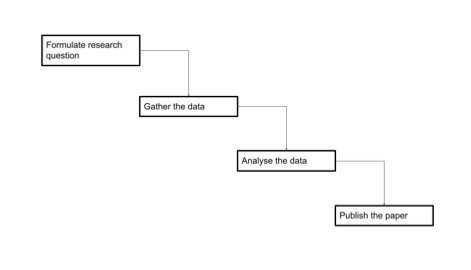
\includegraphics{https://github.com/learnopenscience/TOPS-OC2-data/blob/adb7137694dde403ca54c7b8f755e79dd60fe8d8/assets/Figure5.1.png}

}

\caption{Linear workflow focussed on publications}

\end{figure}

Figure 5.1: Linear workflow model

On the other hand, if one thinks of open data that can be FAIR (and thus
reused) then this model emerges. In particular that Data needs to be
available beyond the publication of a paper. Data no longer has to be
associated with one paper. Data can be reanalysed. More data, from
different sources or the same lab, can be added in at any time,
including later. Instead of the process being a linear progression, with
a start and a finish, the process for data becomes more complex and
there is cycle. These ideas were put together in the
\href{http://www.ijdc.net/article/view/69}{DCC Curation Lifecycle model}
{[}\href{https://doi.org/10.2218/ijdc.v3i1.48}{1}{]}. The original life
cycle is complicated but a summary of the life-cycle is listed below

\begin{figure}

{\centering \includegraphics{https://old.dataone.org/sites/all/images/DLC2015_sm.png}

}

\caption{The DataOne Data life cycle}

\end{figure}

Figure 5.2: A summary of the data life cycle (reproduced from
https://old.dataone.org/data-life-cycle)

Here the focus is very much moved away from the idea of research
-\textgreater{} publication and instead is on the data itself as a first
class research output.

Let's look at these individual steps

\begin{itemize}
\tightlist
\item
  \textbf{Plan}: a description of the data that will be compiled, how
  the data will be managed and made accessible throughout its lifetime.
\item
  \textbf{Collect}: this corresponds to the data gathering step
  (illustrated in Figure 5.1). It can include both primary (raw) and
  processed data.
\item
  \textbf{Assure}: the quality of the data is assured through checks and
  inspections.
\item
  \textbf{Describe}: data is accurately and thoroughly described through
  documentation (e.g.~metadata).
\item
  \textbf{Preserve}: these are the steps necessary to make sure that the
  data will be accessible going forward so in particular ensuring that
  the data is stored in a fashion that others can use it (in particular
  storing at a data repository). Ideally this should be done in a
  fashion that matches the CARE and FAIR principles (lesson 4). This may
  also include the step of removing data that may not be of use to
  future researchers. For example, high resolution images may no longer
  be themselves useful if in the analysis step one has extracted the
  features of interest from them. Not storing the high resolution image
  and simply storing the feature data would provide a considerable
  saving of storage.
\item
  \textbf{Discover}: here other researchers can extract either the
  entirety or some subset of the data for their own purposes.
\item
  \textbf{Integrate}: data from disparate sources are combined to form
  one homogeneous set of data that can be readily analyzed (this could
  include this one data set being analyzed).
\item
  \textbf{Analyze}: corresponds to the data analysis step as illustrated
  in Figure 5.1. There are a variety of different interpretations of the
  data life-cycle (see the reading list for this lesson) with varying
  degrees of complexity. It's also important to note that this is an
  idealization of what goes in general. Nonetheless, it is important to
  think of all these steps as an ongoing, interactive process that
  requires thorough planning and continued consideration and to
  recognize that they are non-trivial to do.
\end{itemize}

\hypertarget{data-management-plans-dmp}{%
\section{Data Management Plans (DMP)}\label{data-management-plans-dmp}}

Seeing as the above steps are not trivial before one begins to gather,
collate or generate a data set it is useful to plan out what you will do
with the data. This is referred to as a Data Management Plan or DMP for
short.

A DMP means that you can think ahead of any particular issues that might
crop up in terms of handling the data, such as the potential cost of
storage, whether data needs to be anonymised and so on.

A detailed description of what one should put into a DMP is described
\href{https://the-turing-way.netlify.app/reproducible-research/rdm/rdm-dmp.html}{here}
{[}3{]}. As outlined in this
\href{https://www.ukri.org/councils/stfc/guidance-for-applicants/what-to-include-in-your-proposal/data-management-plan/}{document
from the UKRI} {[}4{]}, the central funder for the UK, these can include
answering questions such as

\begin{itemize}
\item
  What type of data will be generated or preserved? This could include
  data formats, rough estimates of the amount of data to be stored
  during a research project and similarly what will be preserved beyond
  the lifetime of the project?
\item
  What type of metadata will be used and preserved. It is worth noting
  that one of the more detailed aspects of the FAIR principles is to
  keep the metadata of the data set available even if the original data
  set no longer exists.
\item
  Where should the data be preserved? i.e.~what repository will be used
  (repositories are discussed in the next lesson). How long should it be
  stored? (five years? ten years?) More concretely, data regulations can
  require that certain data be kept in certain ways for at least a
  certain amount of time. This will vary depending on the type of data
  (e.g.~medical records, population statistics). It is advised that
  these expiration dates are explored in the literature, and/or policy
  guidelines.\\
\item
  How will any private data be stored so that it is kept securely?
\end{itemize}

DMPs are not meant to be exhaustive documents! Typically they are 1-2
pages of A4 and often are less than a few thousand words. The important
point is that they sketch out what a researcher or research team plans
to do with their data well before they are gathered and can identify any
steps that need to be taken rather than facing a major challenge now.

DMPs are \href{https://dmptool.org/public_templates}{increasingly used
by funders} and their institutions as a means to have researchers map
out what they will do with their data in a research proposal. Research
proposals often require DMPs, and hence DMPs are often the `sharp end of
the stick' for researchers with respect to Open Science {[}5{]}. A good
DMP is a criterion for assessment in grant applications and hence doing
a good DMP will help your grant be funded.

\hypertarget{documenting-your-data-metadata}{%
\section{Documenting your Data
(Metadata)}\label{documenting-your-data-metadata}}

As discussed in the previous lessons, the FAIR principles emphasize the
importance of metadata, namely documenting your data. Metadata is
described in more detail
\href{https://the-turing-way.netlify.app/reproducible-research/rdm/rdm-metadata.html}{here}
{[}6{]}.

A perennial question is what type of metadata and description of the
data should be provided for a data set. If you are dealing with
electronic data should one provide metadata for a whole set of files, an
individual file \ldots{} each individual bit?

The simplest rule of thumb is if there aren't any guidelines for your
type of data or domain repositories, then try and provide enough
documentation about your data that you would ask for if you were
downloading this data yourself.

For example if this was data taken from a field trip where location is
important then you might want to include longitudinal and latitudinal
coordinates. If it's data from a wet lab then it might include
parameters you normally include in the materials and methods section of
a paper. If it's data from purely computational work you may want to
list the software run and the parameters used.

Data repositories will be discussed in the next lesson. Domain specific
repositories will often give more precise requirements on metadata
(another reason to use them).

If there are no guidelines then a simple README file attached with the
data is a start (for an example see
\href{https://cornell.app.box.com/v/ReadmeTemplate}{here}) - though it's
important to note that ideally one should use metadata schema which is
described in much more detail
\href{https://www.dcc.ac.uk/guidance/standards}{here} as FAIR data
should be machine-actionable {[}7{]} {[}8{]}.

\hypertarget{help}{%
\section{Help}\label{help}}

Much of the ins and outs of dealing with Open Data, or more particularly
Open Data that follows good practice such as the FAIR principles, can be
technical and lies beyond the domain of knowledge of researchers. How
does one navigate this landscape?

This can be summarized in the following diagram -

\begin{figure}

{\centering 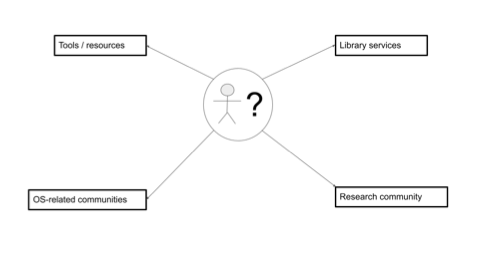
\includegraphics{https://github.com/learnopenscience/TOPS-OC2-data/blob/8509153045f69f2c52c6a6192c52476c54560071/lessons/Figure5.3.png}

}

\caption{Figure 5.3 Diagram pointing to four possible sources of
informaiton a researcher can approach.}

\end{figure}

Figure 5.3 Sources of information and support on Open Data that a
researcher could access.

\hypertarget{research-communities-international-and-national}{%
\subsection{\texorpdfstring{\textbf{Research communities (international
and
national)}}{Research communities (international and national)}}\label{research-communities-international-and-national}}

Individual research disciplines may already have put together materials
and have advice on how to implement Open Science in their discipline.
For example \href{https://fairsharing.org/}{FAIRsharing} is a
educational and information resource on data and metadata standards
{[}9{]}. The \href{https://rd-alliance.org/}{Research Data Alliance}
have a variety of different
\href{https://www.rd-alliance.org/groups}{interest and working groups}
in data sharing in specific disciplines. Scientific Societies and
Publishers can also provide advice {[}10{]} {[}11{]}.

\hypertarget{open-science-related-communities}{%
\subsection{\texorpdfstring{\textbf{Open Science related
communities}}{Open Science related communities}}\label{open-science-related-communities}}

There are a number of communities that are focussed on Open Science
activities. \href{https://reproducibilitea.org/}{ReproducibiliTea} is a
grass-roots journal club initiative that is based in over 100
institutions and is a forum to discuss reproducibility, closely allied
to Open Science {[}12{]}. The \href{https://fairdataforum.org/}{FAIRdata
forum} allows you to browse materials and raise questions that are
related to FAIR {[}13{]}. Correspondingly the
\href{https://pidforum.org/}{PID forum} allows you to ask questions on
PIDs in general {[}14{]}. A list of Open Science communities is provided
in the next module (Open Tools).

\hypertarget{tools-and-resources}{%
\subsection{\texorpdfstring{\textbf{Tools and
resources}}{Tools and resources}}\label{tools-and-resources}}

Finally, there are a range of different tools to help you. For example,
\href{https://dmptool.org/quick_start_guide}{DMPtool} and
\href{https://dmponline.dcc.ac.uk/}{DMPonline} allow you to build your
own DMPs {[}15{]} {[}16{]}. See the module Open Tools for more details.
There are a variety of different catalogs out there one can use to
search for materials in this area.
\href{https://www.sciencedirect.com/science/article/pii/S2666389921001720}{Shanahan,
Hoebelheinrich and Whyte} (2021) have a table of catalogs to search for
materials {[}17{]}.

\hypertarget{local-library-or-it-services}{%
\subsection{\texorpdfstring{\textbf{Local library or IT
services}}{Local library or IT services}}\label{local-library-or-it-services}}

The long term vision is that Higher Education Institutions (HEIs) or
Research Performing Organisations (RPOs)
\href{http://insights.uksg.org/articles/10.1629/uksg.484/}{will employ
data professionals to advise and support researchers} {[}18{]}. These
individuals have a variety of possible job titles such as Data
Librarian, Data Steward, Data Curator and so on. These individuals would
advise on aspects on how to make your data adhere to the CARE and FAIR
principles, providing appropriate metadata and so on. Some HEIs/RPOs
have already made Open Science (or Open Research) policy statements and
may not yet have an infrastructure to help but will be interested in
supporting you. In some countries there has been progress in this area
but it is very early days. Nonetheless, it is worth contacting your
University library as they may be able to advise you even on relatively
small questions or requests.

\hypertarget{summary-13}{%
\section{Summary}\label{summary-13}}

Making data open is not trivial. It is not simply a matter of placing a
data set onto a cloud drive. Nonetheless, if it is done correctly then
the open data is available for reuse. Reuse can be a completely
different research team or it could be the same research team that need
to carry after a member of the team responsible for the data has moved
on. This means one has to think of the data as part of life-cycle and
that it is important to make plans (a Data Management Plan) prior to
creating the data to ensure that it is stored appropriately. Part of
making your data FAIR is provide metadata that describes the data that
you are depositing. Finally, do not feel that you have to do all this
from scratch. There are a variety of different avenues that you can
approach, either on an online basis or sometimes on your own campus.

\hypertarget{assessment-3}{%
\section{Assessment}\label{assessment-3}}

Think about the data sets that were described in lesson 1 as examples of
good data.

\begin{itemize}
\tightlist
\item
  Can you identify what were the above steps with that data?
\end{itemize}

Think now about a data set in your own discipline.

\begin{itemize}
\tightlist
\item
  What would be the steps that you would need to take with that data to
  match up with the data life cycle?
\end{itemize}

\hypertarget{references-6}{%
\section{References}\label{references-6}}

\begin{enumerate}
\def\labelenumi{\arabic{enumi}.}
\tightlist
\item
  Higgins, S. ,''The DCC Curation Lifecycle model'', Intl. J. Digital
  Curation, \textbf{3} (1), 2008, DOI
  \href{https://doi.org/10.2218/ijdc.v3i1.48}{10.2218/ijdc.v3i1.48}
\item
  \href{https://fairsharing.org/}{https://old.dataone.org/data-life-cycle}
\item
  \url{https://the-turing-way.netlify.app/reproducible-research/rdm/rdm-dmp.html}
\item
  \url{https://www.ukri.org/councils/stfc/guidance-for-applicants/what-to-include-in-your-proposal/data-management-plan/}
\item
  \url{https://dmptool.org/public_templates}
\item
  \url{https://the-turing-way.netlify.app/reproducible-research/rdm/rdm-metadata.html}
\item
  \href{https://fairsharing.org/}{https://cornell.app.box.com/v/ReadmeTemplate}
\item
  \url{https://www.dcc.ac.uk/guidance/standards}
\item
  \url{https://fairsharing.org/}
\item
  \url{https://www.rd-alliance.org/}
\item
  \url{https://www.rd-alliance.org/groups}
\item
  \url{https://reproducibilitea.org/}
\item
  \url{https://fairdataforum.org/}
\item
  \url{https://pidforum.org/}
\item
  \url{https://dmptool.org/quick_start_guide}
\item
  \url{https://dmponline.dcc.ac.uk/}
\item
  Shanahan, H., Hoebelheinrich, N., \& Whyte, A. (2021). Progress toward
  a comprehensive teaching approach to the FAIR data principles.
  \emph{Patterns}, \emph{2}(10), 100324.
  \url{https://doi.org/10.1016/j.patter.2021.100324}
\item
  Plomp, E., Dintzner, N., Teperek, M. \& Dunning, A., (2019).
  ``Cultural obstacles to research data management and sharing at TU
  Delft'', \emph{Insights}, \textbf{32}(1),
  \url{http://doi.org/10.1629/uksg.484}
\end{enumerate}

\hypertarget{opensciency-open-data-authors}{%
\chapter{OpenSciency Open Data:
Authors}\label{opensciency-open-data-authors}}

\textbf{Jannatul Ferdish}

\url{https://github.com/Jannatul-Ferdush}

\textbf{Siobhan Hall}

\url{https://github.com/smhall97}

\url{https://twitter.com/smhall97}

\textbf{Pauline Karega}

\url{https://orcid.org/0000-0001-7974-048X}

\url{https://github.com/karegapauline}

\url{https://twitter.com/KaregaP}

\textbf{Steven Klusza}

\url{https://github.com/smklusza}

\textbf{Andrea Medina-Smith}

\url{https://orcid.org/0000-0002-1217-701X}

\url{https://github.com/andreamedinasmith}

\textbf{Esther Plomp}

\url{https://orcid.org/0000-0003-3625-1357}

\url{https://github.com/EstherPlomp}

\url{https://twitter.com/PhDToothFAIRy}

\textbf{Yuhan (Douglas) Rao}

\url{https://orcid.org/0000-0001-6850-3403}

\url{https://github.com/geo-yrao}

\url{https://twitter.com/douglas_rao}

\textbf{Hugh Shanahan}

\url{https://orcid.org/0000-0003-1374-6015}

\url{http://www.shanahanlab.org/}

\part{Open Results}

Welcome to the Open Results Module!

Recap: In Open Ethos, we learned about the ethics and principles
underlying responsible open science practices. In Open Software, we
explored and identified the right tools and methods that allow us to
ensure reproducibility through version control, code testing, workflow,
and a virtual research environment. In Open Data we developed a data
management plan that can ensure the Findability, Accessibility,
Interoperability and Reusability (FAIR) of our data throughout the
research process, and not just at the end when the final report from the
project is released.

In this module, we will explore the different stages of the research
process---including identifying the different types of Research Objects
in a study and the various ways in which they can be shared and
disseminated as open results. We will define a Research Object and
provide an overview of how they relate to the research lifecycle (Lesson
1). Specifically, we will discuss the different stages of the research
process, from ideation and planning all the way through and beyond
dissemination. Then, we will consider how these Research Objects can be
shared (Lessons 2-3). By the end of the module, we will have looked at
the important concepts and practices for publishing and sharing research
components before, during and after the project. Lastly, we address
ethical contributorship, -- making sure collaboration is fair and
inclusive, and that credit is assigned transparently and equitably
(Lesson 4).

\hypertarget{objectives}{%
\section*{Objectives:}\label{objectives}}
\addcontentsline{toc}{section}{Objectives:}

\markright{Objectives:}

\begin{enumerate}
\def\labelenumi{\arabic{enumi}.}
\tightlist
\item
  Identify research stages and elements of research objects that can be
  considered results
\item
  Identify the guiding practices and principles related to open results
  and the advantages of implementing them across stages of a research
  process
\item
  Identify paths for publicly communicating results
\item
  Create open results contributor guidelines and opportunities for open
  and equitable collaborations
\item
  Give credit to contributors in open results
\item
  Contribute and provide constructive feedback to others' results
\item
  Apply open result principles to new and ongoing research projects
\end{enumerate}

\hypertarget{overview-and-key-messages}{%
\section*{Overview and key messages}\label{overview-and-key-messages}}
\addcontentsline{toc}{section}{Overview and key messages}

\markright{Overview and key messages}

This module addresses different questions discussed systematically
across the following four lessons:

Lesson 1: The Research Process and Its Results

\begin{enumerate}
\def\labelenumi{\arabic{enumi}.}
\tightlist
\item
  What are the different stages of the research process?
\item
  What are ``Research Objects''?
\end{enumerate}

Lesson 2: Results in the Context of Open Science

\begin{enumerate}
\def\labelenumi{\arabic{enumi}.}
\tightlist
\item
  What are the advantages of making results open throughout the research
  process?
\item
  What resources are available to help make results open?
\item
  What are the guiding principles to turn a research result into an open
  result?
\end{enumerate}

Lesson 3: Applying Open Result Framework to your Research

\begin{enumerate}
\def\labelenumi{\arabic{enumi}.}
\tightlist
\item
  How can you apply an open framework across different research objects?
\item
  How can you share your results, and select **tools**that support open
  science?
\item
  Using a checklist to achieve open results
\end{enumerate}

Lesson 4: Providing Equitable Opportunities and Credit for Contributors
to Results

\begin{enumerate}
\def\labelenumi{\arabic{enumi}.}
\tightlist
\item
  How can you define contributors to each digital research object and
  determine their suitable form of recognition?
\item
  How can you create contributor guidelines that ensure equity, access,
  inclusion, and diversity?
\item
  How can you ensure your open results are properly attributed and cited
  by others?
\end{enumerate}

\hypertarget{the-research-process-and-its-results}{%
\chapter{The Research Process and Its
Results}\label{the-research-process-and-its-results}}

\hypertarget{introduction-15}{%
\section{Introduction}\label{introduction-15}}

With the overarching goal of maintaining research integrity and ethical
practices from the start, we need to consider reproducibility methods,
collaborative approaches and transparent reporting for the research
teams to ensure that all results can be replicated, validated, and built
upon by other independent researchers. As researchers, this means: 1)
broadening our perspectives regarding what shareable research outputs
are produced throughout the research process, 2) providing sufficient
documentation that describes the research workflow and the
decision-making process, and 3) publishing all research outputs that
would eventually enable others to validate the research findings.

Before we can begin to do that, we need to define what we mean by the
research process, and what we consider research outputs at various
stages of our research. Accordingly, this lesson will enable you to
answer two questions:

\begin{enumerate}
\def\labelenumi{\arabic{enumi}.}
\tightlist
\item
  What are the different stages of the research process?
\item
  What research objects can be considered a result?
\end{enumerate}

\hypertarget{what-is-a-research-object}{%
\section{What is a research object?}\label{what-is-a-research-object}}

A \textbf{Research Object (RO)} is a method for the identification,
aggregation and exchange of scholarly information on the Web
{[}\href{https://www.sciencedirect.com/science/article/abs/pii/S0167739X18314638}{Garcia-Silva
et al.~2019}{]}. RO can be composed of both research data and digital
research objects that are defined as follows by Organisation for
Economic Co-operation and Development
(\href{https://legalinstruments.oecd.org/en/instruments/OECD-LEGAL-0347}{OECD
Legal Instruments}).

\textbf{Research data} consists of ``\emph{factual records (such as
numerical scores, textual records, images, and sounds) resulting from
research that is partially or fully funded by public funds, used as
primary sources for scientific research, and that are commonly accepted
in the scientific community as necessary to validate research
findings.}''

A \textbf{research-relevant ``digital'' research object} consists of any
``\emph{metadata, algorithms, workflows, models, and software (including
code) resulting from research that is partially or fully funded by
public funds, which are used in a research and development context.}''

Research Objects are often given an identifier. In this way, there is a
mechanism to trace back related resources about a scientific
investigation. The most important aspects to consider about ROs:

\begin{itemize}
\tightlist
\item
  They are not only associated with the end products as publications and
  final reports but also encompass research outputs created, revised and
  shared throughout the research lifecycle that help validate findings
  claimed in scholarly publications. More simply, ROs apply to any
  ``single information unit'' or research material that can be
  \textbf{shared and cited} with other scientists within and outside the
  project.
\item
  Motivation behind RO is the need to identify and share all components
  such as data, source code, tools, and method documentation, as well as
  communication materials such as presentations, videos, blogs and other
  tangible outcomes.
\item
  ROs facilitate reproducibility and reuse of the scientific methods and
  results through access to resources, context and metadata
\item
  ROs help us to understand the entire research lifecycle through
  research outcomes including publications shared progressively. They
  also allow us to track the versioning and development of the entire
  project.
\end{itemize}

Ultimately, there are three guiding principles for ROs
{[}\href{https://the-turing-way.netlify.app/communication/research-objects.html}{reference}{]}:

\begin{enumerate}
\def\labelenumi{\arabic{enumi}.}
\tightlist
\item
  Digital identity - Using unique identifiers, such as DOIs (link to
  data) for tangible outcomes such as publications or data, and ORCID
  ids for researchers (explained in detail in the next lesson). This
  enables others to cite and use individual components of your work.
\item
  Data aggregation - Using a method to aggregate all outcomes so that
  they are discoverable and hence allow anyone to investigate and
  reproduce the research.
\item
  Annotation - Use rich machine-readable metadata (discussed in open
  data) that help ensure the findability and accessibility of all
  scientific work.
\end{enumerate}

\begin{figure}

{\centering 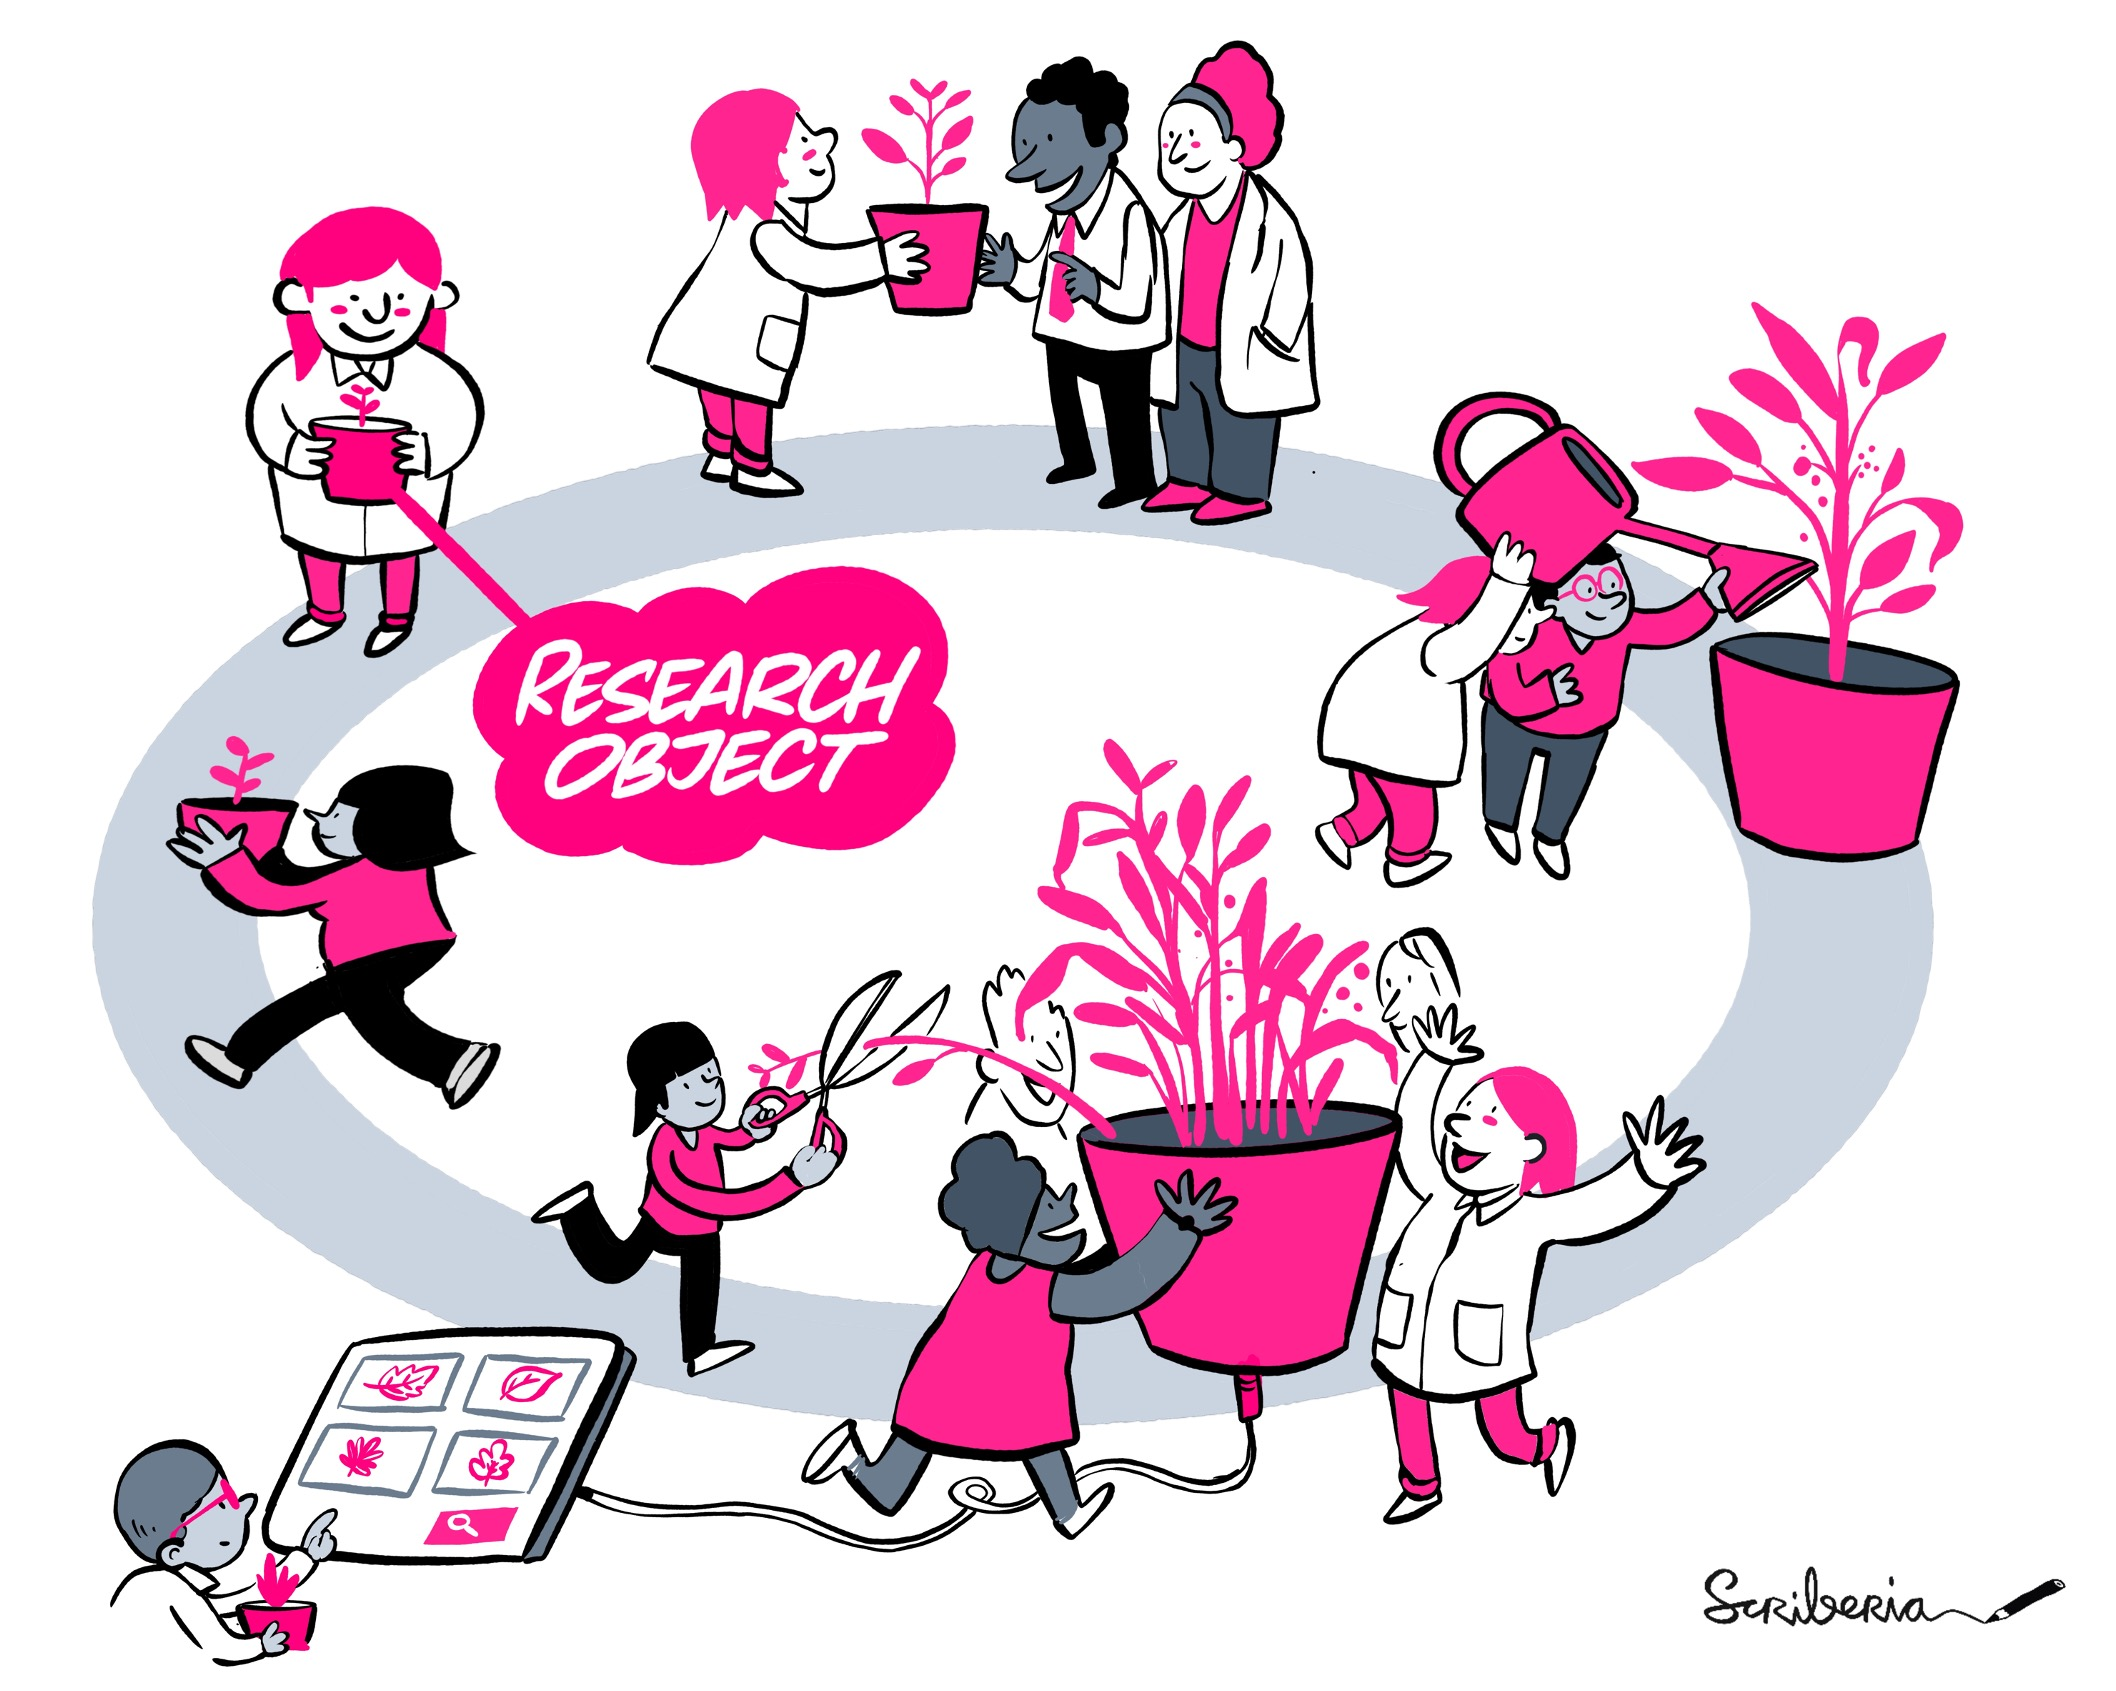
\includegraphics{open-results/figures/research-object.jpg}

}

\caption{This image shows how research objects evolve and grow in
content during the collaboration process and how new research objects
can be derived from existing ones.}

\end{figure}

Figure 1: \emph{Research Objects allow working open by design and share
during the research process and not only the research outputs at the
end. The Turing Way project illustration by Scriberia. Used under a
CC-BY 4.0 licence.
DOI:}\href{https://doi.org/10.5281/zenodo.3332807}{\emph{10.5281/zenodo.3332807}}\emph{.}

Following from these we can now build a definition for an \textbf{Open
Result.}

An \textbf{Open Result} is all the research outcomes, including
successful products, reports on potential risks, experiments that worked
as well as failed, or any other information such as experimental
protocols, standards as well as all the individuals who contributed to
the research can be recorded in the RO and shared as open results.

\hypertarget{what-are-the-different-stages-of-the-research-process}{%
\section{What are the different stages of the research
process?}\label{what-are-the-different-stages-of-the-research-process}}

In previous modules, we have learned the fundamentals and practical
concepts for planning our research for open science. Specifically, in
the Ethos of Open Science {[}addlink-ethos{]} module, we learned that
open science should be considered throughout the research process, and
not just at the time of publication. With this understanding, when
considering shareable research outputs, it is important to think about
the entire research life cycle -- different tasks carried out during the
life cycle of a research project.

Many of us might be very familiar with the research life cycle but may
not have considered what results could be shared openly throughout the
process.

\begin{figure}

{\centering 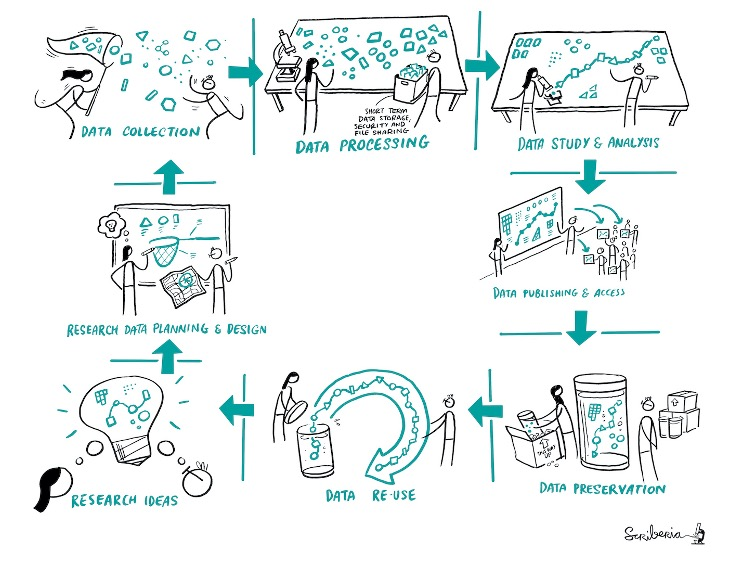
\includegraphics{open-results/figures/research-cycle.jpg}

}

\caption{The research process is represented as a perpetual cycle of
generating research ideas, performing data planning and design, data
collection, and data processing and analysis, publishing, preserving and
hence, allowing re-use of data.}

\end{figure}

Figure 2: \emph{The Turing Way} project illustration by Scriberia. Used
under a CC-BY 4.0 licence.
DOI:\href{https://doi.org/10.5281/zenodo.3332807}{10.5281/zenodo.3332807}.

There are many ways to describe a research life cycle, but in this
lesson, we define it in \emph{nine} distinct phases based on Figure 1
\href{https://the-turing-way.netlify.app/reproducible-research/overview.html}{\emph{The
Turing Way}} that builds on various published examples.

\hypertarget{conceptualizationideation}{%
\subsection{Conceptualization/Ideation}\label{conceptualizationideation}}

In this stage, we focus on outlining and describing the research idea to
different collaborators, students and/or postdocs. This could also
encompass proposal writing, obtaining ethics approval documents, and/or
securing funding.

\hypertarget{planning-1}{%
\subsection{Planning}\label{planning-1}}

In this stage, we are thinking about project management and workflows.
Who is needed for the research project to be successful? During the
planning phase, collaborations are often extended beyond close
collaborators. Methods of collaboration are often defined, including
team member roles and responsibilities.

\hypertarget{project-design}{%
\subsection{Project Design}\label{project-design}}

In this stage, we are concerned with describing the research protocols.
For example, what the research hypothesis is, what protocols will be
used to conduct the study, how will the data be collected, and
processed, where will it be stored, and more.

\hypertarget{data-collection}{%
\subsection{Data Collection}\label{data-collection}}

In this stage data collection (from publicly available databases or
resources) or data generation (through experiments or
quantitative/qualitative studies) commence. See Open Data
{[}addlink-data{]}.

\hypertarget{data-wrangling-and-processing}{%
\subsection{Data Wrangling and
Processing}\label{data-wrangling-and-processing}}

At this stage, we use existing software or write custom code to process
the data that has been collected. See Open Software
{[}addlink-software{]}.

\hypertarget{data-exploration-and-statistical-analysis}{%
\subsection{Data Exploration and Statistical
Analysis}\label{data-exploration-and-statistical-analysis}}

At this stage, we combine the workflows from Stages 4 and 5 and begin
using our tools, code or software to analyse the data that has been
obtained.

\hypertarget{reporting}{%
\subsection{Reporting}\label{reporting}}

Here we report on our findings, in other words, we share them with the
research community. This can be done in the form of a research
manuscript first published on a preprint server and in a peer-reviewed
journal. However, reporting now far exceeds publication alone. Reporting
also encompasses presentation materials (such as posters, and slide
decks), lab websites or blogs, outreach materials for social media,
podcasts or press releases, and many more.

\hypertarget{preservation-and-reuse}{%
\subsection{Preservation and Reuse}\label{preservation-and-reuse}}

In this stage, we consider archiving all outcomes for long-term
preservation. This ensures that our research is accessible, and
reusable, meaning that someone else can go through this whole process of
reproducing or building upon our work.

\hypertarget{scientific-engagement-training-and-feedback-cross-cutting}{%
\subsection{Scientific Engagement, Training, and Feedback
(cross-cutting)}\label{scientific-engagement-training-and-feedback-cross-cutting}}

In this stage, we conduct effective collaboration through active
engagement, skill development and peer-review processes for both direct
and indirect stakeholders of our research.

\textbf{Important note:} Although we describe these stages in sequential
order, these stages may not always be linear. For instance, scientific
engagement and data management efforts will be applied at all stages of
research. Data exploration, analysis and reporting will be an iterative
process, and reporting will happen at different points of the research
lifecycle. Even before the study begins, research questions, hypotheses,
and planned approaches may be openly reported or preregistered
{[}\href{https://www.pnas.org/doi/10.1073/pnas.1708274114}{Nosek et
al.~2018}{]}. Preregistration differentiates research outcomes which are
the results of predictions, which occur before data collection, from
predictions, which occur once the results of the data are obtained.

To build high-quality research outcomes, it is essential that everyone
(1) can work together efficiently at all stages of the project, (2) has
a shared understanding of how results from their work will be shared
with each other, and more broadly beyond the project, and (3) gets
fairly recognized for all their contributions.

\hypertarget{what-research-objects-are-commonly-associated-with-research-stages}{%
\section{What research objects are commonly associated with research
stages?}\label{what-research-objects-are-commonly-associated-with-research-stages}}

Now that we understand the different stages of the research lifecycle,
Research Objects and open results, we can expand on how they operate in
the context of the research lifecycle. The most important outcome to
consider is that these ROs can be produced throughout the research
lifecycle and should be published throughout, rather than at the end of
the research process.

\hypertarget{research-stages-and-open-result-table}{%
\subsection{Research stages and open result
table}\label{research-stages-and-open-result-table}}

\begin{longtable}[]{@{}
  >{\raggedright\arraybackslash}p{(\columnwidth - 2\tabcolsep) * \real{0.5000}}
  >{\raggedright\arraybackslash}p{(\columnwidth - 2\tabcolsep) * \real{0.5000}}@{}}
\toprule()
\begin{minipage}[b]{\linewidth}\raggedright
\textbf{Research Stages}
\end{minipage} & \begin{minipage}[b]{\linewidth}\raggedright
\textbf{Possible research objects as open results}
\end{minipage} \\
\midrule()
\endhead
Conceptualization and planning & Proposal, ethics approval document,
budget/funding plan, contributor and partnership plans (see lesson 4
{[}addlink{]}), preregistration reports, research materials, research
protocol \\
Project design & Versioning system, shared project repository, project
planning document (project goals, roadmap, ways of working, roles and
responsibilities, communication), hypothesis and pre-registration,
collaboration plan, Equity, Diversity, Inclusion and Accessibility
(EDIA) guidelines, data management plan, metadata standards, governance
plan, data safety and security guide \\
Data collection & File formats and data types, parameters/dimension,
test data, metadata, data access plan/details, raw data \\
Data wrangling and processing & Statistical methods, tools, workflow and
analysis pipeline, processed data, code for data exploration,
statistical results \\
Data exploration, statistical analysis & Notebooks, figures, code,
software package (R package, python library), code documentation,
models, technical reports on scope and limitation of data, configuration
and virtual research environment \\
Engagement, training, and feedback from peers (communications and
collaboration) & Contribution guideline (feedback documents, process for
inviting feedback), review sprint plan and outcomes, departmental and
conference talks, user testing information, tutorials, executable
notebooks, videos \\
Preservation and reuse (Research Data Management) & Data management plan
with the versioning system, metadata standards, data governance and
archiving plans, data sharing and archiving information, code packages,
virtual research environments, hardware (if produced), physical
samples \\
Reporting, publication & Posters/figures, talks/slides, preprints,
journal/book publications, layman summary, lab website/blogs, outreach
materials for social media, podcast/press release, containers for
testing (Docker, Binder), documentation and manuals, research compendia,
configuration files (for reproducibility), software release information,
hardware plan and associated documentation \\
\bottomrule()
\end{longtable}

\hypertarget{contributions-that-are-not-research-objects-but-should-be-considered-as-results-and-recorded-openly}{%
\subsection{Contributions that are not Research Objects but should be
considered as results and recorded
openly}\label{contributions-that-are-not-research-objects-but-should-be-considered-as-results-and-recorded-openly}}

Research, like most technical professions, involves different kinds of
contributions that do not always result in tangible outcomes and hence,
can't always be defined by RO. For example, responsibilities associated
with maintenance of RO, community management, data stewardship, library
and archiving work, ``Equity, Diversity, Inclusion and Accessibility''
(EDIA) efforts, as well as tasks associated with funding, project
management, scientific event organization, training activities and more.
Outcomes from these roles cannot always be accurately captured besides
documenting their processes, methods and impact, often recorded by some
people involved in those roles. In Lesson 4, we discuss how to properly
acknowledge the contributors to your results.

\hypertarget{assessment-1-identify-the-research-objects-in-your-project-or-a-case-study}{%
\section{Assessment \#1: Identify the research objects in your project
or a case
study}\label{assessment-1-identify-the-research-objects-in-your-project-or-a-case-study}}

Invite project ideas from the learners and the broader open science
community before delivering the training.

\hypertarget{self-assessment-2-identify-the-research-objects-to-be-shared-as-open-results-of-a-project-you-arewere-involved-in}{%
\section{Self-assessment \#2: Identify the research objects to be shared
as open results of a project you are/were involved
in}\label{self-assessment-2-identify-the-research-objects-to-be-shared-as-open-results-of-a-project-you-arewere-involved-in}}

Provide an empty version of the ``research stages and open result
table'' table to be filled by the learners.

\hypertarget{conclusion}{%
\section{Conclusion}\label{conclusion}}

The research consists of many different stages, each with several
important tasks. In the early stages, we deal with Conceptualization and
Planning. This can include a number of different things - depending on
the project - but typically involves the development of a study
protocol, research questions, and other study materials. Next, comes
Project Design. In this stage, we often focus on developing a study
timeline (or roadmap), assigning different roles to project team
members, creating data and metadata management plans, and planning for
data collection, management, and security. Next, is the active
responsibility for Data Collection. Taking a step back from a project
can help us establish an understanding of this multifaceted process and
give us an appreciation of all the important elements (and people)
involved in bringing a project or study from conceptualization through
to completion and dissemination. In the next lesson, we will consider
the advantages - for ourselves and the broader scientific community - of
making our results open and transparent. In doing so, we will explore
best practices for transforming our work from closed to open.

\hypertarget{references-7}{%
\section{References}\label{references-7}}

\begin{enumerate}
\def\labelenumi{\arabic{enumi}.}
\tightlist
\item
  The Turing Way Chapters: Guide for Reproducible Research and Research
  Object to capture the Research Life Cycle,
  \url{https://the-turing-way.netlify.app/welcome.html}, The Turing Way
  Community, Zenodo, 27 July 2022, doi:10.5281/zenodo.6909298.
\item
  Garcia-Silva, Andres, et al.~``Enabling FAIR research in Earth Science
  through research objects.'' Future Generation Computer Systems,
  vol.~98, 1 Sept.~2019, pp.~550-64, doi:10.1016/j.future.2019.03.046.
\item
  ``OECD Legal Instruments.'' 25 Aug.~2022,
  legalinstruments.oecd.org/en/instruments/OECD-LEGAL-0347.
\item
  Nosek, Brian A., et al.~``The preregistration revolution.''
  Proceedings of the National Academy of Sciences, vol.~115, no. 11, 13
  Mar.~2018, pp.~2600-2606, doi:10.1073/pnas.1708274114.
\end{enumerate}

\hypertarget{results-in-the-context-of-open-science}{%
\chapter{Results in the Context of Open
Science}\label{results-in-the-context-of-open-science}}

\hypertarget{introduction-16}{%
\section{Introduction}\label{introduction-16}}

In the previous lesson, you learned that the results of a research
project encompass much more than just a published paper. In this lesson,
we will demonstrate the benefits and challenges of making your research
results open.

You will learn that making results open entails making them findable,
accessible, interoperable, and reusable (FAIR) while caring for both
people and purpose. To this end, we will discuss available guiding
principles to enhance the usefulness of your research results for you as
a researcher, for your research team, for your collaborators and for
society in general. Applying these principles requires key changes in
the practice and culture of research and the implementation and
normalisation of certain technologies and practices that will be covered
in the next two lessons as well.

Some research projects produce sensitive research objects that cannot be
shared due to ethical, legal, technical or institutional reasons. We
will discuss how your research project can be reproducible and
collaborative without necessarily having them all open.

\hypertarget{what-are-the-advantages-of-making-results-open-throughout-the-research-process}{%
\section{\texorpdfstring{What are the \textbf{advantages} of making
results open throughout the research
process?}{What are the advantages of making results open throughout the research process?}}\label{what-are-the-advantages-of-making-results-open-throughout-the-research-process}}

In the Ethos of Open Science module, we discussed the general benefits
of Responsible Open Science {[}addlink-ethos{]}. In this section, we
will link how these advantages pertain to each Research Object (RO)
learned in Lesson 1 {[}addlink-results1{]}. In order to simplify the
discussion we will merge the possible ROs in four big categories:

\begin{itemize}
\tightlist
\item
  \textbf{Preparation documents.} This category includes all outcome ROs
  from the research project planning phases, for example, ideation \&
  conceptualization, planning and project design
\item
  \textbf{Datasets.} This includes raw or processed datasets from the
  following research stages: data collection, data wrangling and
  processing, and preservation and reuse. \emph{Additional information
  about the advantages of making data open can be found in the Open Data
  module {[}addlink-data{]}.}
\item
  \textbf{Software.} This refers to all the software created and used in
  all research stages, in particular: data collection, data wrangling
  and processing, data exploration \& analysis and Preservation and
  reuse. \emph{Additional information about the advantages of making
  software open can be found in the Open Software module
  {[}addlink-software{]}.}
\item
  \textbf{Reports.} This category includes all ROs associated with
  communicating results within the research group or/and outside, e.g
  Communication, reporting and publications
\end{itemize}

The main identified advantages of making results open are the following:

\begin{enumerate}
\def\labelenumi{\arabic{enumi}.}
\tightlist
\item
  \textbf{Avoids duplicating efforts}.\hspace{0pt} \emph{This is
  important for all types of ROs}.
\end{enumerate}

For example, a single dataset can be analysed in multiple ways. Another
example is that the same implementation of the data processing,
exploration and analysis stages (including but not limited to analysis
pipeline, statistical methods, tools, and software) can be reused for
another phase of the same project or for a new project without the need
of reimplementation by each researcher.

\begin{enumerate}
\def\labelenumi{\arabic{enumi}.}
\tightlist
\item
  \textbf{Saves time and increases efficiency.} \emph{This is important
  for all types of ROs}.
\end{enumerate}

If the research project is open from the start, it can help you to be
more efficient and save a considerable amount of time (see the Ethos for
Open Science module for ``planning for open science''
{[}addlink-ethos{]}). First, having the preparation documents open will
guarantee that all members of the team have at hand the information
about the project design and planning big picture. Second, you save time
when you are required to share your dataset, methods and software with
funders and publishers. Third, an open workflow creates efficient
pipelines from the start. Fourth, open ROs from the Engagement, feedback
and reporting stages can also significantly improve the review process
by validating the results available at each research stage within or
outside your team. This improves replicability, as independent
researchers can replicate and confirm the results at each step. Good and
open documentation of data, codes and scripts, protocols and
intermediate results will speed up writing your final
papers/publications.

\begin{enumerate}
\def\labelenumi{\arabic{enumi}.}
\tightlist
\item
  \textbf{Facilitates collaboration and onboarding of new members.}
  \emph{This is also important for all ROs}.
\end{enumerate}

\textbf{Collaboration} will be much easier when preparation documents,
datasets, methods and software are open and well-documented. Having user
testing, tutorials, executable notebooks and videos from the
``Engagement, training, and feedback stage'' will be additionally
important for \textbf{onboarding} new members of your team or external
collaborators. Your research project will be easier to be continued by
you (even after some changes in the composition of your group) or by a
different research group.

\begin{enumerate}
\def\labelenumi{\arabic{enumi}.}
\tightlist
\item
  \textbf{Allows collaborators to receive credit, and provides
  incentives for others to contribute.} \emph{This is important for all
  kinds of ROs}.
\end{enumerate}

Making your results open also opens you up to clearer ways of
\textbf{receiving credit} and can also reduce the risk of scooping (each
result can be individually referenced as soon as made available).
Applying reproducibility practices separately on different parts of the
project such as \textbf{Preparation documents, datasets, software and
reporting} allows other researchers to test and reuse your work in their
research, and your research will be more cited thus bringing fair
recognition for your work. Collaborators can get more \textbf{motivated
to contribute} because they can easily get recognition in terms of
authorship for their contributions made for each one of the ROs
generated.

\begin{enumerate}
\def\labelenumi{\arabic{enumi}.}
\tightlist
\item
  \textbf{Furthers the reach and audience of our results.} \emph{This is
  particularly related to the Communication and collaboration, reporting
  and publishing steps}
\end{enumerate}

Open posters/figures, talks/slides, preprints, webpages, and
journal/book publications will allow more members of your academic
community to access your research, which in turn can turn into more
collaboration and recognition and a greater impact of your research
results. But the impact can be extended outside the academic community
as well by also making available public summaries, lab websites/blogs,
social media, podcast/press releases, and citizen science projects among
others which can strengthen the link with the local community and enrich
your research.

\begin{enumerate}
\def\labelenumi{\arabic{enumi}.}
\tightlist
\item
  \textbf{Funding.} Since more and more funding agencies are paying
  attention to open science and requiring applying guiding open science
  principles to the research project they fund, open practices will make
  you \textbf{eligible for more funding opportunities}.
\end{enumerate}

The picture below summarises the most significant advantages for all
actors in the research ecosystem of making your results open.

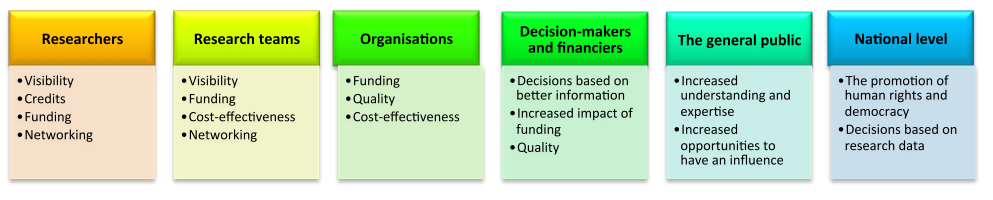
\includegraphics{open-results/figures/benefits.png}

(reference: @factorsoecd)

\hypertarget{what-are-potential-obstacles-and-what-resources-are-available-to-help-overcome-them}{%
\section{What are potential obstacles and what resources are available
to help overcome
them?}\label{what-are-potential-obstacles-and-what-resources-are-available-to-help-overcome-them}}

\hypertarget{overall-potential-obstacles}{%
\subsection{Overall Potential
Obstacles}\label{overall-potential-obstacles}}

Along with all the clear benefits of open results, there is a suite of
real and perceived challenges. These obstacles were described in the
Ethos module {[}addlink-ethos{]} and can be divided into two categories:

\begin{itemize}
\tightlist
\item
  External obstacles: \textbf{cultural barriers} (lack of support and
  recognition from your institution), \textbf{disagreement} between
  collaborators involved in the research on what results to make open,
  \textbf{legal} and \textbf{security} considerations;
\item
  Internal obstacles: investment of \textbf{time} and \textbf{effort}
  needed upfront to make your results open including the need to learn
  additional \textbf{skills}, afraid of scooping, the lack of
  \textbf{funding} for instance for open-access publications and
  curating research results.
\end{itemize}

These obstacles apply to any Research Objects (created by you or your
collaborators), for example, data, software and documents, reports and
publications.

Let's focus on results that are not software or data. You can check the
Data {[}addlink-data{]} and Software {[}addlink-software{]} modules for
any questions specifically related to open data and software.

One of the major steps in research is the communication of your ideas
and insights from your work into a clear, open, and accessible format
that can help key stakeholders make meaningful decisions. Mastering
different ways to convey your insights responsibly is challenging and
can be seen as a diversion to your research work: blogging, writing
public summaries, podcasting, presenting posters and talks at
conferences outside of your discipline, and using social media requires
communication skills that are not usually taught to students, and can be
extremely time-consuming while the impact is very difficult to measure.

\hypertarget{obstacles-and-recommendations-for-open-access-reporting}{%
\subsection{Obstacles and Recommendations for Open Access
Reporting}\label{obstacles-and-recommendations-for-open-access-reporting}}

The most common way to communicate research results is by far their
publication in journals. However, the choice of a journal or a
publishing platform may affect the availability and accessibility of the
research results.

Open Access publications allow you to make available articles and/or
books accessible online, free of charge to the public without any
restriction (no mandatory registration or log in to specific platforms
required). Publishing your results in Open access journal is a good way
to increase your research impact and allows everyone, including society
as a whole, to use your research results.

However, publishing open access can incur additional costs that may not
be covered by your research grant or institution. Before publishing to a
journal, check if there are institutional open access agreements in
place: the costs are usually significantly reduced and sometimes you may
be able to publish Open Access with no additional cost. Several
publishers also offer waivers and discounts to researchers living in
low- and middle-income countries. Other cost-offsetting programs may be
available too: for instance, some publishers have a fee support program
to ensure that accepted articles can benefit from open access.

In many disciplines, there are also Open Access Journals where the
content is open for everyone, with no need to pay or be a member of a
subscribing institution. The number of these journals is still
increasing rapidly and you can search open access journals and articles
in the Directory of Open Access Journals
\href{https://www.doaj.org/}{DOAJ}.

You may choose to self-archive your research results to make them more
discoverable and/or after you've published them in a subscription
journal to ensure there is an open version of your paper. Preprint
servers are also increasingly popular: you can deposit documents that
have not been peer-reviewed in a traditional journal-led process but are
considered a complete scientific publication in the first stage. Some of
the preprint servers include open peer review services and the
availability to post new versions of the initial paper once reviewed by
peers. Preprints can be used to share a paper before it is submitted to
a journal and can reduce scooping. Many publishers accept this as a
standard practice but some may reject papers which have been shared in
preprint form. It's therefore important you read carefully the
publisher's policies when considering submitting a paper.

Finally, in most cases, you can also self-archive your publications in
repositories, including \href{https://zenodo.org/}{Zenodo}. It is
however recommended to check if the journal has any specific
self-archiving policy. Your institution may also have an institutional
repository. Check the \href{http://roar.eprints.org/}{Registry of Open
Access Repositories} to search and find an up-to-date list of available
repositories.

More information about open access for other research objects like data
and software have been discussed in Open Data and Open Software modules
respectively.

\hypertarget{obstacles-with-being-open-when-reusing-closed-research-objects-by-others}{%
\subsection{Obstacles with being open when reusing closed Research
Objects by
others}\label{obstacles-with-being-open-when-reusing-closed-research-objects-by-others}}

We have detailed the most common challenges you may face when making
your results open. Additional challenges may arise if you reused closed
Research Objects (ROs) but want to make your results open. Below are
examples and possible solutions to overcome these challenges:

\hypertarget{potential-obstacle-1}{%
\subsubsection{Potential obstacle 1}\label{potential-obstacle-1}}

you do not get consent from some of your collaborators for opening some
datasets you have used in your analysis.

\textbf{Recommended solution}: you can create and share metadata
(description of the content, data format, link to sample data files)
instead. However, your results may not be reproducible. Therefore when
sharing your workflows and software, it would be useful to provide
sample datasets to demonstrate the reusability of your work. We
recommend you agree early on (at the planning stage) on what datasets
you will be using and whether they are open or will be opened (embargo).

\hypertarget{potential-obstacle-2}{%
\subsubsection{Potential obstacle 2}\label{potential-obstacle-2}}

your research work involves the usage of sensitive datasets that cannot
be shared when publishing.

\textbf{Recommended solution}: make sure to detail clearly the protocol
used to collect the dataset and the condition of access. Ensure you have
metadata to increase the FAIRness of your work. You may also want to
provide sample datasets (for example, anonymized) to ease reuse and
support the creation of derivative work.

\hypertarget{potential-obstacle-3}{%
\subsubsection{Potential obstacle 3}\label{potential-obstacle-3}}

The software you have used for your analysis is not open. This will of
course limit the reproducibility of your results to those who can access
the software you used.

\textbf{Recommended solution}: if it is commercial software, you can add
metadata information such as the software name, version, and
prerequisites (see software module {[}addlink-software{]}) to help
others to identify and possibly buy the very same software. The more
costly the software is, the less likely your research results will be
reproduced and reused. When the software is closed and/or available at a
cost, it is recommended to add sufficient information on the algorithm
used to make it more accessible. If possible, provide containerized
executable versions or offer an online service to run the software.
Whenever you start a project, you should assess the tools you would need
and evaluate the impact of using close or commercial software.

\hypertarget{what-are-the-guiding-principles-to-turn-a-research-result-into-an-open-result}{%
\section{What are the guiding principles to turn a research result into
an open
result?}\label{what-are-the-guiding-principles-to-turn-a-research-result-into-an-open-result}}

Following the FAIR principles (see Ethos module {[}addlink-ethos{]}) can
help ensure research results are Findable, Accessible, Interoperable and
Reusable. This is one of the prerequisites to making research results
open and available to everyone. The CARE principles (Collective benefit,
Authority to control, Responsibility and Ethics) are also detailed in
the Ethos module and complement the FAIR principles: they are people and
purpose-oriented and aim at advancing the Indigenous peoples' rights and
self-determination.

For Data and/or Software Research Objects, you can read the Data and
Software Modules, respectively. Other types of Research Objects such as
your planning and research results documents (for example, data
management plan, project proposals, blogs, and videos) and publications
need to follow the FAIR principles to allow others to understand your
work and eventually derive new creative work.

Before learning how to ensure your research results are FAIR, let's
clarify the concept of FAIR and highlight the differences between FAIR
and Open.

\textbf{FAIR for Closed Research Objects}

Ideally, Research Objects should be FAIR and Open. However, it is not
always possible. For instance, whenever there is sensitive data or data
that cannot be distributed (for example, it could harm or target
specific people or identify the location of endangered species or
animals), sufficient metadata can make the RO FAIR while keeping the
data itself closed. Therefore, Research Objects can be \textbf{FAIR but
not open}.

\textbf{FAIR for Open Research Objects}

Openness is a necessary but not sufficient condition for maximum reuse.
When the content of Research Objects can be made open without harming
anyone and with the consent of all the contributors, ensuring their
FAIRness increases reproducibility and reuse.

\hypertarget{transforming-an-unfair-to-fair-result}{%
\subsection{Transforming an ``unFAIR'' to ``FAIR''
result}\label{transforming-an-unfair-to-fair-result}}

Here we will explore two scenarios:

\begin{enumerate}
\def\labelenumi{\arabic{enumi}.}
\tightlist
\item
  The Research Object is not yours
\item
  The Research Object has been created by you and your research team.
\end{enumerate}

\hypertarget{turning-someone-else-research-object-into-a-fair-result}{%
\subsubsection{Turning someone else Research Object into a FAIR
result}\label{turning-someone-else-research-object-into-a-fair-result}}

\begin{itemize}
\tightlist
\item
  Check the license of the Research Object: if you cannot share the
  content, you can still create metadata.
\item
  Add metadata (authors information, size of the Research Object,
  contact information, title, description, and location such as a
  persistent identifier or Digital Object Identifier) with detailed
  information about the Research Object itself. Readme tools such as
  \url{https://readme.so/} can help guide building informative metadata
  {[}addlink-tools{]}
\item
  Deposit the Research Object (if it can be re-distributed) in a
  repository where you can add metadata and get a persistent identifier
  such as Zenodo or a community-specific repository. If the Research
  Object itself cannot be redistributed, creating a record in a
  repository such as Zenodo where you can add as much metadata as
  necessary for others to understand and potentially request the
  Research Object itself.
\end{itemize}

\hypertarget{turning-your-research-object-into-a-fair-result}{%
\subsubsection{Turning your Research Object into a FAIR
result}\label{turning-your-research-object-into-a-fair-result}}

\begin{itemize}
\tightlist
\item
  Check the colours of your figures and tables and change them to make
  them colourblind-friendly (see for instance
  \url{https://www.color-blindness.com/coblis-color-blindness-simulator/}).
\item
  Check that making available your research results will not potentially
  harm anyone. In doubt, do not open the particular research result.
\item
  Tidy your project structure to use descriptive file names and logical
  folder structure. See this resource for a good summary of what makes
  for good file names and folders:
  \url{https://datamanagement.hms.harvard.edu/collect/file-naming-conventions}
\item
  Add a README file to your folders to explain what they contain. This
  tool can help easily build a readme: \url{https://readme.so/}
\item
  Move data saved in proprietary formats to open standards (for
  instance, move files saved in DOCX format to RTF or HTML).
\item
  Add code and code documentation, with descriptions of what each
  function does, and what their inputs and outputs are, and include
  examples. See open software for documentation standards
  {[}addlink-software{]}.
\item
  When publishing data, add an example of how to read and analyse the
  data.
\item
  Upload reports in open archives.
\item
  Choose Open-Access platforms that give free and online availability of
  research outputs.
\item
  Publish a blog or a video abstract in simple language for the
  layperson.
\item
  Link all the contents of your research outputs as an aggregated
  Research Object (for example, ensure data, code, and metadata can be
  found in the same archive).
\item
  Add any other relevant metadata (add effective title/names,
  description and keywords) to each of your research outputs.
\item
  Deposit the aggregated Research Object into a repository that can
  deliver persistent identifiers such as Digital Object Identifier.
\end{itemize}

\hypertarget{the-continuum-from-closed-to-open}{%
\subsection{The continuum from closed to
open}\label{the-continuum-from-closed-to-open}}

All research results lie on a scale between closed and open because
there are variances in how information is shared and the reasons to
share. Your research results can be:

\begin{enumerate}
\def\labelenumi{\arabic{enumi}.}
\tightlist
\item
  \textbf{Closed}. It is only available to certain individuals within an
  organization. It is patented or proprietary.
\item
  \textbf{Mediated}. It is semi-restricted to certain groups or it is
  open to the public through a licence fee or other pre-requisite. As we
  have discussed in previous sections, there are legitimate reasons to
  restrict access to data and when data is mediated possible users must
  request access. For example, health-related information collected by a
  hospital or insurance carrier
\item
  \textbf{Embargoed}. The result will be open in the future. For
  example, some groups might release their data following an appropriate
  latency period to allow a thorough understanding of the data as well
  as to allow time for the scientific exploitation of the data by the
  research team.
\item
  \textbf{Open}. It is accessible in a readable format and licensed as
  open source.
\end{enumerate}

And there are many setups in between these four categories!

\hypertarget{aggregating-your-research-objects}{%
\subsection{Aggregating your Research
Objects}\label{aggregating-your-research-objects}}

To work Open you may have created different Research Objects such as
data, software and workflows. The Data and Software modules explained
how to deal with these research results and obtained for instance
Digital Object Identifiers for each of them. When publishing, additional
material can be added (for example, software, data, workflows) but you
usually limit the Research Objects to what is discussed in the paper.
Failures, dead-ends and other trials and errors are part of the research
process and usually do not have their place in scientific publication.
To ease re-use and facilitate the creation of derivative work, you can
aggregate all your research objects to create bundles that represent the
entire research process and not only the selected positive results.

\hypertarget{assessment-case-study-analysis}{%
\section{Assessment: Case study
analysis}\label{assessment-case-study-analysis}}

\begin{enumerate}
\def\labelenumi{\arabic{enumi}.}
\tightlist
\item
  Building on self-assessment \#2 in Lesson 1. Which of those elements
  were guided by FAIR principles?
\item
  Flag the research objects you think could benefit from FAIR
  principles.
\item
  Rank order those objects from ``would benefit most from FAIR
  principles'' to least
\item
  Rank order those objects from ``would require most resources'' to
  least
\item
  Identify a few research objects that strike a balance between high
  priority and resources required
\end{enumerate}

\hypertarget{applying-open-result-framework-to-your-research}{%
\chapter{Applying Open Result Framework to your
Research}\label{applying-open-result-framework-to-your-research}}

\hypertarget{introduction-17}{%
\section{Introduction}\label{introduction-17}}

After the previous section, you're probably raring to go to make your
research objects as findable, accessible, interoperable and reusable as
you can. But how can you go about actually doing so? In this section, we
will delve deeper into the practical issues of open results and
introduce some specific tools and services that will get you 80\% of the
way there.

Bear in mind that no tool is optimal in every context. All
recommendations made in this lesson are based on what is generally
useful but might not be ideal for your particular domain of research,
institutional context, culture or legal framework. When in doubt, you
can ask your relevant community (for example, the relevant people in
your institution, your colleagues and your peers) what tools are
available, validated and recommended (See Tools for in-depth discussion
on Open Communities {[}addlink-tools{]}).

Also of note, these tools are not neutral. All of them are developed and
maintained by people in the English-speaking developed world, which
charges them with biases and assumptions that might not be relevant to
your own situation.

\hypertarget{how-to-apply-an-open-framework-across-different-research-objects}{%
\section{How to apply an open framework across different research
objects}\label{how-to-apply-an-open-framework-across-different-research-objects}}

An open result is the aggregation of all the research objects introduced
in the last lesson (software, data, workflows, reporting, documents).
Ideally, to open your research results you would need to open each
Research Object that you can legally and ethically open and aggregate
them into your final Research result. The approach you need to follow to
open an individual Research Object is independent of the type of
Research Object (RO) even though the tools may be very different. Below
we introduce the main concepts that are necessary to open your Research
Objects. Later, we will go through each type of research result
(document-RO, data-RO, executable-RO, reporting-RO) and learn the most
popular tools you can use.

\hypertarget{unique-identifiers}{%
\subsection{Unique identifiers}\label{unique-identifiers}}

Perhaps the single most important step to make your results open is to
assign them a globally unique and persistent identifier. This will give
you a single code, URL or number that you can use to uniquely refer to
the research object unambiguously. Any derived research object can use
this identifier to link to it and create a traceable and rich history of
use and development. Crucially, this identifier can be used by others to
cite and credit your work.

The identifier must also be persistent. This guarantees that the
identifier points to the same research object for a long time. What
counts as ``persistent'' is, of course, a matter of degree since even
the most stable identifier probably won't survive the Sun engulfing the
Earth in a few billion years. In this context, ``persistent'' implies
that it is registered in a database managed by an organisation or system
that is committed to maintaining it stable and backwards compatible for
the foreseeable future.

For example, URLs (for example, a personal website, GitHub repository,
or cloud storage) are notoriously not persistent since they can change
their contents frequently or become invalid without maintenance. On the
other hand, Journal publications have a Digital Object Identifier, whose
persistence is guaranteed by the International DOI Foundation.

As well as uniquely identifying each research object, it is important to
be able to uniquely identify and cite all the authors and contributors.
For this, it is recommended to get the permanent digital ID of each of
the authors and contributors. \href{https://orcid.org/}{ORCID} (Open
Researcher and Contributor ID) is an online service where you can get a
permanent digital identifier.

Exercise:

(multiple choice) Select which of the following are globally unique and
persistent identifiers:

\begin{itemize}
\tightlist
\item
  ✅ Digital Object Identifier 10.1371/journal.pone.0230416

  \begin{itemize}
  \tightlist
  \item
    The Digital Object Identifier is provided by the International DOI
    Foundation, which ensures that each ID is unique and ensures that a
    DOI link always links to the correct object.
  \end{itemize}
\item
  ❌ \url{https://github.com/alan-turing-institute/the-turing-way}

  \begin{itemize}
  \tightlist
  \item
    This is the URL of a GitHub repository. The contents of the
    repository can drastically change over time and the owner can delete
    it completely.
  \end{itemize}
\item
  ✅ ISBN-13: 978-0735619678

  \begin{itemize}
  \tightlist
  \item
    This is an International Standard Book Number, which has to be
    purchased by publishers by the International ISBN Agency.
  \end{itemize}
\item
  ✅
  \url{https://web.archive.org/web/20220121051903/https://www.go-fair.org/}

  \begin{itemize}
  \tightlist
  \item
    The Internet Archive captures snapshots of websites and their links
    are really stable. Even if not ideal, it's a handy tool for creating
    identifiers of websites easily.
  \end{itemize}
\end{itemize}

\hypertarget{metadata-1}{%
\subsection{Metadata}\label{metadata-1}}

The second step to make your research objects open is to produce textual
information \emph{about} the research object (metadata) and link to it.
This metadata serves both humans and machines. For humans, having
metadata is imperative to ease understanding. For example, it can
contain variable names contained in a dataset, physical units of a
variable of a dataset, the software used to generate and/or read the
dataset, the training method of a machine learning model, and the
sampling method used for a particular dataset. For machines, metadata is
useful for indexing and searching, as well as programmatically
interacting with digital research objects. To be ``understood'' by
machines, metadata must follow established conventions and/or standards
that are often domain specific. To make your data, software, and
workflow interoperable, mapping metadata standards from different
disciplines and/or creating cross-disciplinary standards is often
necessary but a very complex procedure.

In general, try to think about what information you would need to have
in order to know if that research object is relevant to your needs.
However, some metadata information that applies to almost any research
object is:

\begin{itemize}
\tightlist
\item
  Title: A short but descriptive sentence that introduces the research
  object.
\item
  Description: A longer text with a more thorough description of the
  research object. This might include descriptions of the process that
  created it, important caveats or limitations, and anything that you
  think would be useful to contextualise it.
\item
  Authors: A list of people responsible for creating the research object
  and who should be credited if it is used.
\item
  Contributors: A list of people who contributed to populate the content
  of the Research Object and/or the original authors when you create
  derivative work from another existing Research Object.
\item
  Date of creation/publication: Try to use an unambiguous date format
  like the ISO 8601 year-month-day format.
\item
  Version: a number or other sort of ID that helps disambiguate between
  different versions of the research object, in case it is updated (for
  instance, if you found an error after publishing it).
\end{itemize}

As mentioned earlier, many domains have adopted formal metadata
standards. To facilitate interoperability between domains the Research
Data Alliance (RDA) develops and maintains
\href{https://rdamsc.bath.ac.uk/}{the RDA Metadata Standards Catalog}, a
collaborative, open directory of metadata standards applicable to
research data.

These guidelines we give for each type of Research Object are not domain
specific and should be considered as the minimum required for making
your research results open. In any case, metadata should always be open
even though you cannot share the associated content (for instance for
sensitive datasets and/or closed software).

Exercise:

(multiple choice) Select which pieces of information would be included
in the metadata of a dataset of species, sex, body mass, height, flipper
length, and bill length measured at three Antarctic Islands

\begin{itemize}
\tightlist
\item
  ✅ Date of the data collection.

  \begin{itemize}
  \tightlist
  \item
    When the data were collected can be important for
    ecological/longitudinal studies.
  \end{itemize}
\item
  ✅ Geographical coordinates of each island.

  \begin{itemize}
  \tightlist
  \item
    The location of the islands can be used for spatial analysis and
    also for indexing.
  \end{itemize}
\item
  ❌ Average height of all penguins.

  \begin{itemize}
  \tightlist
  \item
    This can be computed from the data itself.
  \end{itemize}
\item
  ✅ Make and model the scale used to collect weight measurements.

  \begin{itemize}
  \tightlist
  \item
    Instrument details are important to assess the quality of the
    measurements.
  \end{itemize}
\item
  ✅ Filename and extension of the files.

  \begin{itemize}
  \tightlist
  \item
    Descriptive filenames are very useful for humans to understand the
    contents of a file and can contain important information, such as
    dates or locations. The file extension can be used as a good
    heuristic to know how to read its contents.
  \end{itemize}
\item
  ✅ Software name and version.

  \begin{itemize}
  \tightlist
  \item
    Descriptive information about the software you used for producing
    and/or analysing data is crucial for reuse. See ``Software module''
    {[}addlink-software{]} for more comprehensive information about
    Software release, documentation, and testing.
  \end{itemize}
\end{itemize}

\hypertarget{licencesrules-for-reuse}{%
\subsection{Licences/Rules for reuse}\label{licencesrules-for-reuse}}

Another very important element to include with your research objects is
clear rules for reuse (as is and for creating derivative work), which
are often and most easily codified by the use of licences.

Without a licence, all rights are with the author of the research
result, and that means nobody else can use, copy, distribute, or modify
the work without consent. A licence gives this consent. If you do not
have a licence for each of the research objects that constitute your
research result, it is effectively unusable by the whole research
community.

Choosing a licence is not always straightforward, especially since your
institution might have legal requirements. If you are using other
people's work, you also need to pay attention to their licences and
choose one that is compatible. Different types of licences can be used
and the choice also depends on the type of Research Object: licences for
software (executable research object) are very different than for
documents. We recommend checking the Data module, and software module to
get a better understanding of the licences you can use for each type of
Research object. In this lesson, we will recommend the most common
approach for each type of RO.

To guide you in your choice, you can use Choose a licenced website:
\url{https://choosealicense.com/}

For instance, if your Research Object is not software, attaching a
Creative Commons Attribution 4.0 International gives permission to
anyone to share and modify your research object as long as they credit
you.

In the context of Research Results, we also recommend being consistent
in the usage of the licences for all the different Research Objects you
aggregate into your final Research results. For instance, if you choose
a permissive licence for your dataset but a closed licence for the
software needed to read the data, you significantly reduce the usage of
your dataset.

\hypertarget{how-to-share-your-results-and-select-tools-that-support-open-science}{%
\section{How to share your results, and select tools that support open
science?}\label{how-to-share-your-results-and-select-tools-that-support-open-science}}

Here we will go through each stage of the research cycle defined in the
categories of Lesson 2 and discuss how you can share each of the
components. First, it is important to understand: what is a repository,
and why it is important to register research objects in a searchable
resource:

\hypertarget{repositories}{%
\subsection{Repositories}\label{repositories}}

All the above needs services that can assign unique identifiers and link
them to the research objects and associated metadata, including the
licences. Repositories are services that cover all those bases.

Zenodo is a very popular repository (Yeston 2021) in which you can
register metadata and obtain a Digital Object Identifier, as well as
host digital objects such as data, code and publications.

\href{https://reliance.rohub.org/}{RoHub} is a Research Object registry
where you can create Research Objects and aggregate Research results
stored/deposited in different repositories.

\hypertarget{registering-in-a-searchable-resource.}{%
\subsection{Registering in a searchable
resource.}\label{registering-in-a-searchable-resource.}}

If you use a service such as Zenodo and/or RoHub, your Research results
will be automatically searchable, for instance in
\href{https://explore.eosc-portal.eu/}{EOSC Explore}.

Being able to find a research object and understand its contents through
its metadata is a great step. But it can be lost if the person who found
the data is not able to access it.

For humans, providing detailed information on where to start, and what
to look at in the aggregated Research results as well as in each
Research Object, is key. Then, as mentioned earlier, pay attention to
the font, colours (colourblind friendly palettes) and overall use of
simple sentences that can be understood by non-english natives are a few
of the recommendations you can follow. When a Research Object has
private content (such as sensitive data), it is important to provide as
many details as necessary to let other researchers know how to request
data (clearance procedures, instructions on how to register and
authenticate to servers hosting the data). For machines, standardised
APIs (Application Programming Interfaces) are necessary to be able to
access the metadata and data programmatically.

As before, while we will point you to solutions that can work a lot of
the time, we encourage you to check with your institution, which might
already have the infrastructure set up. Also, check which repository is
mostly used in your community.

As you know from Lesson 1, the scope and variety of research objects are
extremely large, so it's impossible to give guidelines (even brief ones)
for all of them. Below we focus on four broad types of research objects.

\hypertarget{documents}{%
\subsection{Documents}\label{documents}}

Sharing all the documentation related to a project helps other
researchers to understand the objectives and can bring further
collaborations. Try to make open everything needed for your research
project proposal, planning and during execution: proposal, ethics
approval, preregistration, project planning, and data management plans.

Recommended tools:

\begin{itemize}
\tightlist
\item
  Upload to Zenodo with CC-BY 4.0 license for archiving and long-term
  preservation.
\item
  Use Google docs or Overleaf for collaboration.
\end{itemize}

\hypertarget{data-1}{%
\subsection{Data}\label{data-1}}

Sharing data, especially large data, is not a solved problem (see the
Open Data section for more in-depth guidance {[}addlink-data{]}). But if
your datasets are small enough and don't carry privacy issues, it's
relatively straightforward to upload them to a repository. Zenodo
(zenodo.org) allows you to upload datasets of up to 50Gb (larger
datasets can be hosted but you need to ask permission) and it provides
you with a unique identifier as well as a whole set of metadata.

Choose a format that is simple to use and read. Make sure to use a data
format that can be read with free software and prefer open standards to
closed formats (for example, plain CSV files are better than excel). If
there is a trade-off between efficient storage and ease of use,
prioritise accessibility, since storage is generally cheap. Some
research communities have developed or embraced particular formats as
their standards so your data will be much more accessible to your
intended audience if you adapt to those.

Recommended tools:

\begin{itemize}
\tightlist
\item
  Upload to Zenodo. Check if both the data and metadata can be shared
  and open whenever you can use the CC-BY-4.0 license. The repository
  allows for datasets as large as 50Gb. Larger datasets can be hosted if
  you ask.
\item
  Check if your domain has some standard and a domain-specific
  repository.
\end{itemize}

\hypertarget{software}{%
\subsection{Software}\label{software}}

If your analysis is code-centric, one of the best steps you can take to
make your code more open is to develop it in a repository with a version
control system. This will not only add transparency to the process but
make collaboration much easier (after the initial investment in learning
the new tool).

GitHub (github.org) is one popular remote repository system for open
source projects. You can create repositories for your projects that can
even be private and with special permissions for internal collaborators.

A GitHub repository is not an archival service nor does it provide a
unique and persistent identifier. To release your code, you need to
create a stable snapshot. To do this, you can connect Zenodo to your
GitHub account to create DOIs of specific snapshots.

Besides where to host the code, an important aspect is documentation.
The single most helpful piece of documentation is to include a README
file that explains what the code does, how it can be installed and how
it's used. To encourage collaboration from outside sources, you can also
include contribution guidelines.

Recommended tools:

\begin{itemize}
\tightlist
\item
  Host your code on GitHub for development and collaboration.
\item
  Connect your GitHub repository to Zenodo and create software releases
  (snapshots) to get their own DOI for release.
\end{itemize}

Exercise:

Think of a specific research object from a project you are/were involved
in and use \url{https://readme.so/editor} to create a README template
that applies to it.

\hypertarget{reports}{%
\subsection{Reports}\label{reports}}

As a scientist, you are probably trained to write and publish papers.
However, traditional publishing outlets are not open, since they require
hefty subscription fees or per--article payments.

Publishing your articles in an Open Access journal might be the easiest
option to make documents open, but most Open Access journals charge
article processing fees that can be prohibitively high. A free
alternative is to upload your manuscript to a preprint server, where you
can upload manuscripts before acceptance to a journal.

A very popular and long-running preprint server is ArXiv
(\url{http://arxiv.org/}). ArXiv is mainly used in physics and computer
science, so you might want to search for a more specialised one for your
community. For biology, there's bioRxiv (biorxiv.org/) and for Earth
sciences, there's EarthArXiv (\url{https://eartharxiv.org/}). Some
journals provide one-click pre-print services upon submission.

If you or your team have a website, consider uploading your report
there. Although simple, the main disadvantage of this is that an
unstructured website doesn't provide unique identifiers and stable links
like a preprint server do.

Something important to consider is what are you allowed to do with a
manuscript that is published in a journal. Some journals don't allow you
to make the final copy-edited version public or even the version with
changes based on peer review.

Beyond publications, you probably want to communicate your research work
to a larger audience. Writing blogs, developing tutorials and/or making
short videos are becoming more and more popular, and an integral part of
the research work.

Recommended tools:

\begin{itemize}
\tightlist
\item
  Upload to a preprint server such as ArXiv. Ask around in your
  community for a more specialised server.
\item
  Upload the report, videos and/or blogs to your personal or
  institutional website.
\end{itemize}

\hypertarget{putting-everything-together}{%
\subsection{Putting everything
together}\label{putting-everything-together}}

Each individual Research Object is now FAIR or as FAIR as you can, and
now it is time to create one aggregated Research Object that constitutes
your final research result (final being here used as complete).

The creation of this aggregated Research Object could be as simple as a
single text or markdown file with all the links to each individual
research result. You can upload that file on your personal or team
website.

However, a more structured alternative is to use a registry of Research
Objects such as \href{https://reliance.rohub.org/}{RoHub}
(\url{https://reliance.rohub.org/}). There you can add links to all the
individual Research Objects that constitute your research result. The
type of Research Object depends on the main constituents of your final
Research Result. We usually recommend creating an executable Research
Object for aggregating all your research results. Each Research Object
has a persistent identifier. Once created and ready to be published, you
can make snapshots and ultimately archive your Research Object to get a
Digital Object Identifier. When you create a Research Object in RoHub,
it is harvested in OpenAire and your research result is automatically
searchable in \href{https://explore.eosc-portal.eu/}{EOSC Explore}.

Examples

\begin{itemize}
\tightlist
\item
  Executable Research Object
  ``\href{https://w3id.org/ro-id/435f534c-e49b-43c3-9bd6-3393100bef3f}{Cosmos-UK
  soil moisture (Jupyter Notebook) published in the Environmental Data
  Science book}''
\item
  Data-centric Research Object
  ``\href{https://w3id.org/ro-id/61bceafe-5b48-4548-8caf-4142153b1b1b}{Mean
  ground velocities from ALOS-2 data at Changbaishan volcano
  (China/North Korea) during 2018-2020}''
\item
  Bibliography-centric Research Object
  ``\href{https://w3id.org/ro-id/e1d32110-086e-4de3-80b2-21dfe6ae068a}{The
  effects of the Covid-19 pandemic seen through the lens of the Italian
  university teachers and the comparison with school teachers'
  perspective}''
\end{itemize}

Recommended tools:

\begin{itemize}
\tightlist
\item
  Create a Research Object in RoHub (https://reliance.rohub.org/)
\end{itemize}

\hypertarget{as-open-as-possible-as-restricted-as-necessary}{%
\subsection{As open as possible as restricted as
necessary}\label{as-open-as-possible-as-restricted-as-necessary}}

Reproducibility, and therefore FAIR, should be considered as a guiding
principle in all stages of your research process. But reproducibility
does always mean open. We share the idea that research should be as open
as possible and as closed as necessary (Turning FAIR into reality, EC,
2018). Open principles should be applied when you can and never for
private, confidential or sensitive results.

This does not contradict all that you have learned so far in this module
because FAIR does not require your research objects to be open but it
requires open metadata and open standards for interoperability.

\hypertarget{using-a-checklist-to-achieve-open-results}{%
\section{Using a checklist to achieve open
results}\label{using-a-checklist-to-achieve-open-results}}

The first step to making your research results open is to register to
\href{https://orcid.org/}{ORCID}to get a permanent digital ID for
yourself. We also strongly encourage you to ask all your collaborators
to do the same.

The table below summarises some initial steps that correspond to the
{[}Minimum Viable Solution{]} (see lesson 2) to make your Research
result open. You need to apply these recommendations for each Research
Object that is part of your Research results.

\begin{longtable}[]{@{}
  >{\raggedright\arraybackslash}p{(\columnwidth - 8\tabcolsep) * \real{0.2000}}
  >{\raggedright\arraybackslash}p{(\columnwidth - 8\tabcolsep) * \real{0.2000}}
  >{\raggedright\arraybackslash}p{(\columnwidth - 8\tabcolsep) * \real{0.2000}}
  >{\raggedright\arraybackslash}p{(\columnwidth - 8\tabcolsep) * \real{0.2000}}
  >{\raggedright\arraybackslash}p{(\columnwidth - 8\tabcolsep) * \real{0.2000}}@{}}
\toprule()
\begin{minipage}[b]{\linewidth}\raggedright
\textbf{MVS}
\end{minipage} & \begin{minipage}[b]{\linewidth}\raggedright
F
\end{minipage} & \begin{minipage}[b]{\linewidth}\raggedright
A
\end{minipage} & \begin{minipage}[b]{\linewidth}\raggedright
I
\end{minipage} & \begin{minipage}[b]{\linewidth}\raggedright
R
\end{minipage} \\
\midrule()
\endhead
Documents & Choose an explicit title, write an abstract and add
keywords. & Deposit your document (project proposal, ethics approval,
preregistration, project planning document Data management plans,
others) in a repository such as Zenodo where a DOI is assigned & Avoid
proprietary format and write your document in Plain text (markdown,
LaTeX). For collaboration, you can use HackMD, overleaf or Google Docs.
& Use an Open Licence such as CC-BY-4 \\
Data & Add explicit information (metadata) along with your data. Use
descriptive filenames. Use standards (if they exist) for naming the
variables, and standard physical units for variables. & Deposit your
data in a repository such as Zenodo where a DOI is assignedMake an
example of how to use your data (for instance a Jupyter notebook to read
data) & Avoid using data formats that require the usage of closed or
commercial software. Use data standards that are long-lasting. & Use an
Open licence such as CC-BY-4. See Data Module {[}addlink-data{]} \\
Software & Add information about dependencies, and computational
environment necessary for running the software. & Use a code repository
such as Github or software that is open source. Write tutorial, README,
training material, and contribution guidelines. Write workflows with all
the steps of your analysis. & Use Open source programming languages,
write portable code and share your workflows. & Use an Open Licence such
as an MIT licence. See Software Module {[}addlink-software{]}. Make
internal/external reviews, and write documentation. \\
Reports & Choose an explicit title, write an abstract and add keywords.
& Write publications, blogs, and press releases, and create accessible
graphs (colourblind friendly). & Writing and collaboration: overleaf,
google docs, among others. Avoid proprietary formats for storing your
report. & Use Open Access. \\
\bottomrule()
\end{longtable}

\hypertarget{assessment-case-study-analysis-1}{%
\section{Assessment: case study
analysis}\label{assessment-case-study-analysis-1}}

\begin{enumerate}
\def\labelenumi{\arabic{enumi}.}
\tightlist
\item
  From Lesson 3, consider the three highest-priority research objects
  that could benefit from openness: 1. Identify possible platforms where
  these research objects could be hosted 2. Identify any modifications
  to this research object that would enable it to abide by principles of
  openness
\end{enumerate}

\hypertarget{providing-equitable-opportunities-and-credit-for-contributors-to-results}{%
\chapter{Providing Equitable Opportunities and Credit for Contributors
to
Results}\label{providing-equitable-opportunities-and-credit-for-contributors-to-results}}

\hypertarget{introduction-18}{%
\section{Introduction}\label{introduction-18}}

\begin{quote}
\textbf{If I have seen further it is by standing on the shoulders of
Giants.}

\emph{Turnbull, H. W. ed., 1959. The Correspondence of Isaac Newton:
1661--1675, Volume 1, London, UK: Published for the Royal Society at the
University Press. p.~416}
\end{quote}

If you are a researcher, regardless of your career stage, chances are
you are not working alone. And even if you are working alone on any
given project, your work likely builds on the work of others. And just
like that, others after you will build on your work, advancing our
understanding of the world and beyond.

In the previous lessons of this module, we defined open results and
talked about ways you can frame your research so that all your outputs
are open. We also spent some time explaining why sharing your results
openly avoids ``reinventing the wheel'' by reusing existing work, saves
time and increases efficiency, and facilitates collaboration and
onboarding of new members.

In this lesson, we will talk about authorship and contributorship, and
dive deeper into why open results matter, specifically talking about how
openly communicating your results can open up doors to unforeseen
opportunities for collaborations. We will also provide you with
guidelines on how to ensure contributions to your current or future work
happen equitably, maximizing the chances of fair and successful
collaborations. Finally, we will briefly go over how you can contribute
to others' open results in a way that helps your colleagues improve
their work and work towards shared research goals.

\hypertarget{how-do-we-define-contributors-to-each-research-object-and-determine-their-suitable-form-of-credit}{%
\section{How do we define contributors to each research object and
determine their suitable form of
credit?}\label{how-do-we-define-contributors-to-each-research-object-and-determine-their-suitable-form-of-credit}}

\hypertarget{defining-authors-and-contributors-to-your-project}{%
\subsection{Defining authors and contributors to your
project}\label{defining-authors-and-contributors-to-your-project}}

Too often conversations about contribution and authorship take place
towards the end of a project or right when a scientific publication is
drafted. However, as we learned in the previous lessons, research
outputs are generated throughout the lifetime of a research project. To
share them as open results in different stages of research, we should
build an agreement for how authorship and contributorship in the project
will be managed. This requires collaboratively defining what is
considered authorship in your project, who among the current
contributors is going to get authorship, who will get acknowledged as a
contributor, who goes first and last in the list of a scientific
publication, and who makes these decisions.

First and foremost, we need to remember that \emph{anyone} who has
contributed to the research project must have their contributions
recognized. With that shared understanding, in this lesson, we will
explore what those recognitions as contributors or authors in your
research project might look like.

\textbf{First, let's define what a contributor is:}

A \textbf{contributor} of research output is an individual who has
contributed to any activity that made it possible for the open result to
be published or shared. This includes the person(s) who first
conceptualized the idea and designed the work, the project lead,
external advisors, general mentors, the students, researchers, research
assistants who conducted or helped conduct the experiments, the people
who set up the tools essential for conducting the research, data
stewards, the software developers, support staff, the project management
team, the colleague(s) who provided feedback to the open results, as
well as any collaborator.
{[}\href{https://the-turing-way.netlify.app/collaboration/shared-ownership/shared-ownership-projects.html}{reference}{]}

Depending on the type of contributions, some of these people should be
recognized as authors of the open result, while others are appropriately
acknowledged as contributors.

\textbf{Now, let's define authorship:}

According to the definition provided by the International Committee of
Medical Journal Editors (ICMJE) which is widely accepted in biomedical
disciplines:

An \textbf{author} of an open result is a contributor who has given a
substantial contribution to the conception or design of the work or the
acquisition, analysis, or interpretation of the data for the work.
Additionally, an author is a contributor who has contributed to drafting
or revising critically the work providing important intellectual
content. An author is also someone who has approved the final version of
the open result and agrees to be accountable for all aspects of the work
and for the integrity of all other co-authors.
{[}\href{https://www.icmje.org/recommendations/browse/roles-and-responsibilities/defining-the-role-of-authors-and-contributors.html}{reference}{]}

There are several other definitions of authorship which vary across
disciplines and describe how they relate to different research outputs.
For instance, the
\href{https://publicationethics.org/files/COPE_DD_A4_Authorship_SEPT19_SCREEN_AW.pdf}{COPE
Authorship Discussion Document} indicates that minimum requirements for
authorship are 1) substantial contribution to carrying out the work and
2) accountability for the work conducted and shared in a publication.
Authoring a research manuscript that is published in a peer-reviewed
journal, for example, is widely considered one of the most valuable
currencies for career advancement, promotion, funding opportunities, and
overall chance of being recognized by the research community.

Given the weight traditionally placed on authorship in scientific
publication and the fuzziness of the definitions (that often contain
relative terms such as ``substantial'' or ``extensive'' leaving too much
room for interpretation), it is not surprising that determining who
amongst the contributors gets to be an author can lead to biased or
unfair decisions, disputes between contributors, or at the very least
leave someone resentful and feeling unappreciated.

To avoid these challenges, in the next section, we are going to provide
some tips on how to determine who amongst the contributors is recognized
as an author, as well as how to ensure all contributions to the open
result are recognized fairly beyond authoring papers.

\hypertarget{how-to-fairly-determine-authorship-contributions}{%
\subsection{How to fairly determine authorship
contributions}\label{how-to-fairly-determine-authorship-contributions}}

We established that \_all\_\_contributors to an open result should be
acknowledged for their contributions\_. That said, the research team
should first decide who amongst the contributors gets to be recognized
as an author and how all the other ``non-author'' contributors are
properly acknowledged in the open result (next section).

The National Institute of Health (NIH) provides a useful schematic
representation to help with the first decision (Learn more: Colbert, M.
C., Nussenblatt, R. B., \& Gottesman, M. M. (2018). Integrity in
Research: Principles for the Conduct of Research. Principles and
Practice of Clinical Research (Fourth Edition). Academic Press. doi:
\href{https://www.sciencedirect.com/science/article/pii/B9780128499054000034?via\%3Dihub}{10.1016/B978-0-12-849905-4.00003-4}):

\begin{figure}

{\centering 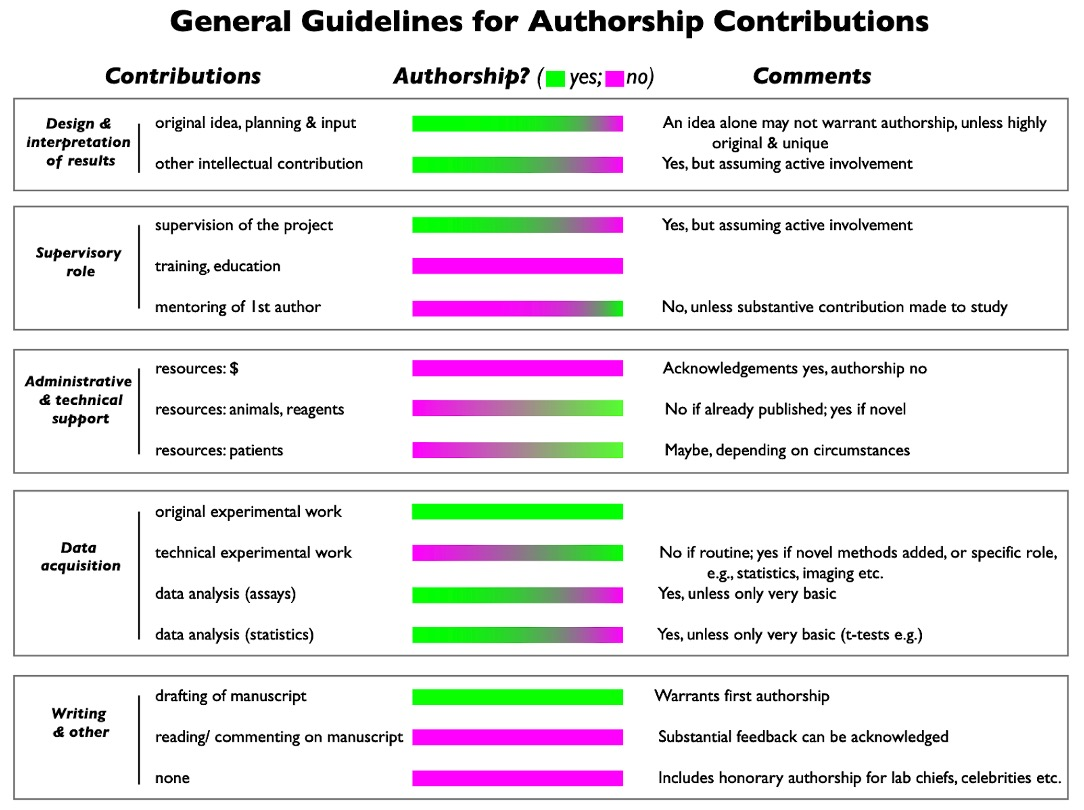
\includegraphics{open-results/figures/authorship-guide.jpg}

}

\caption{General guide for authorship contributions should be given
based on contribution, originality, and active involvement. Authorship
and aknoledgement should be decided on case by case basis for all stages
of research cycle.}

\end{figure}

\emph{Figure 1: Example authorship guidelines from NIH:
\url{https://oir.nih.gov/system/files/media/file/2021-08/guidelines-authorship_contributions.pdf}
(Colbert et al, 2018) DOI:
\href{https://doi.org/10.1016/B978-0-12-849905-4.00003-4}{10.1016/B978-0-12-849905-4.00003-4}}

Even if guidelines like this one can help establish authorship and
contributorship(see others cited below), it is rarely an easy ``yes-no''
(or for the image: ``purple and green'' decision). The power imbalance
between project leads and students, for example, can often mean that
members treated unfairly are the contributors with the least power.

Power dynamics amongst the team of contributors need to be acknowledged
and discussed openly. Hierarchies and power imbalances can be due to
many factors. The most obvious and somewhat accepted in academia are
levels of seniority: those with more experience, and those who have been
around longer tend to hold the most power. But other, sneakier factors
are the legacy of a whole set of systems and structures that have
oppressed groups of people for longer than we can remember. Academia and
science are no exception. These systems of oppression include sexism,
racism, white supremacy, heterosexism, ableism, and many more. It is
important to recognize the implications of living in a society where
people with less power and privileges continue to get disadvantaged by
those systems and to become aware of the resulting biases that may
consciously or unconsciously affect our choices.

We can even go further and try our best to correct those biases by
intentionally deciding to make up for some of the inevitable
shortcomings of which we may be unaware or may not have the lived
experience.

\textbf{That is bringing an equity lens to our work.}

Equity is another word for fairness or levelling the playing field.
\textbf{Equity} is an approach that recognizes that the magnitude of
systemic barriers posed to a particular person will vary based on their
gender identity, race, geographic location, class, age, ability, sexual
orientation and other factors. Equity recognizes that different people
will need different amounts of resources or support to succeed and
overcome these barriers.

If you decide to bring an equity lens to this discussion, consider how
you, with your powers and privileges, may be able to help others get a
seat at the table. Let's say, for example, that you are a postdoc and
the leading author of a research project. A rotating student spends 4
months in the lab helping you set up and perfect the experimental
protocol that you will then use to carry out the experiments needed to
answer your research question. They may even help you collect some
preliminary data, but then they leave and later decide to join another
lab. It may be tempting to not include them as authors in the final work
and not even acknowledge them as contributors---which would be
unethical. However, if you think that they have provided significant
help and contributed to the success of your experiment, you should
consider giving them authorship, perhaps contacting them to help write
the methods section of the manuscript. You would give this student a
huge opportunity to be cited and seen as a professional researcher.

Another aspect that can lead to unfair and unethical authorship
recognition is the position of the author in the author list. Usually,
the first author slot is reserved for the main contributor who has
provided the largest contribution to the open result, someone who has
been responsible for the work ideation, implementation, and completion
carrying it all the way to publication. The last author is generally the
group leader or principal investigator who has overseen the project from
ideation to completion, providing mentorship and substantial
contribution to the open result composition. The authors in the middle
tend to be grouped as all the other contributors who have passed the
``authorship test'', while disregarding the specific contribution each
of them made to the project. Once again it seems that even if a
contributor is recognized as an author, every time an open result is set
to be published or shared, there is an opportunity for the genuine
mistake, misunderstandings, and even plain exploitation and unethical
behaviour {[}Fleming, N., 2021{]}.

One of the best ways to avoid conflicts and unfair authorship
assignments is to \emph{be intentional about it and plan ahead} by
creating an authorship and contributorship document or guideline for
your project!

Below are some tips to guide you in implementing your version of a more
ethical and just authorship assignment approach by \textbf{establishing
authorship and contributor guidelines for your research group}
{[}\href{https://the-turing-way.netlify.app/communication/aa/aa-tips.html}{reference}{]}
\textbf{.}

\begin{itemize}
\tightlist
\item
  \textbf{Search for existing guidelines} (some are linked in this
  lesson) and use them as a starting place to create your own set of
  guidelines. In doing so, seek advice from open science colleagues
  where you are (starting with librarians).
\item
  \textbf{The guidelines should include language to help guide the
  discussion around explicit recognition of power dynamics.} These are
  not easy conversations and having language in the guidelines that
  acknowledge the need for having a conversation around power dynamics
  helps make it happen as part of the shared norms of the group. This
  can include prompts to assess the position of the contributor within
  the team (such as the principal investigator (PI) whose name is
  attached to the grant funding, the student who just joined the group,
  and the staff scientist who has worked in the lab for 4 years) and
  their role and responsibilities in the context of the project
  implementation (such as the student is the one who wrote the first
  draft of the research proposal and is going to carry out the
  experiments, the PI co-wrote and submitted the research proposal and
  will supervise the whole project, the staff scientist is the one who
  is going to carry on the statistical analysis and the postdoc is going
  to help mentor the new student and teach them the technique).
\item
  \textbf{Make sure all members of your research group have the
  opportunity to contribute to the guidelines.} You can draft the
  initial document, but then ask for constructive and honest input from
  the other members of your team. If new members join, make sure they
  are properly onboarded and have a chance to comment on the existing
  guidelines, especially if they are brought in as contributors to an
  ongoing project.
\item
  \textbf{Re-evaluate and seek explicit agreement over the guidelines at
  the beginning of every new research project.} If someone does not
  agree to the guidelines, try to mediate an open conversation about why
  they don't agree, trying to find a common ground amongst the
  contributors. If the disagreement remains, you can consider having
  your team vote and follow what the majority chooses.
\item
  \textbf{The guidelines should include instructions for contributors on
  how to report unethical deviations from the policy} to someone other
  than the group leader (this could be the Chair of the department, a
  dedicated office at the research institution, or the funder of the
  project).
\item
  \textbf{At the time of publication of the open result check for any
  existing policy associated with the platform used for publication
  (such as provided by a journal).} If the policy does not align with
  yours, present your reasoning and negotiate with the platform. Also
  make sure that if the criteria you use to determine authorship
  deviate, you have a space to clearly state the change in the open
  result.
\item
  \textbf{Make the guidelines publicly available.} If you have a group's
  website you can post it there, and/or you can decide to create a
  version of the record and point to a permanent identifier such that
  the link never breaks by publishing the guidelines on a public
  repository (such as GitLab/GitHub or
  \href{https://zenodo.org/}{Zenodo}).
\end{itemize}

Speaking of power imbalances, one thing you may be wondering if you are
not the group leader is, \emph{how on earth am I going to bring this up
to my research group is not at all on board with open science practices
or simply has never thought of having explicit authorship and
contributorship guidelines?} Well, there is no one right way to do this,
but one suggestion we can give you is to learn about it and then present
an outline of the guidelines to your next group meeting. Even if the
work should not be on one person, oftentimes the main barrier to having
something done is to initiate discussion and create that initial draft
to which others can contribute. So, if you are up for it and are
committed to implementing open results practices, we recommend that you
take that first step and then try to persuade others to join in. In most
cases, your colleagues will be grateful and hopefully contribute to
composing the guidelines. Check out the lesson on why and incentives for
additional resources around the benefits of adopting open science
practices (as discussed in the Ethos of Open Science module
{[}addlink-ethos{]}).

\hypertarget{resources-for-additional-contexts}{%
\subsubsection{Resources for additional
contexts}\label{resources-for-additional-contexts}}

\begin{itemize}
\tightlist
\item
  The Contributor Roles Taxonomy or CRediT
  (\url{https://credit.niso.org/}) is a high-level taxonomy that is
  increasingly being used to attribute different kinds of contributions
  made to scientific scholarly output. These include
  \hspace{0pt}\hspace{0pt}\hspace{0pt}\hspace{0pt}conceptualization,
  data curation, formal analysis, funding acquisition, investigation,
  methodology, project administration, resources, software, supervision,
  validation, visualization, writing of original draft, reviewing, and
  editing. In practice, the success of this authorship approach relies
  on all authors openly acknowledging the importance of everyone's
  contributions
  (\href{https://livingwithmachines.ac.uk/highlighting-authors-contributions-and-interdisciplinary-collaborations-in-living-with-machines}{see
  an example by Living with Machine team}).
\item
  The Committee on Publication Ethics (COPE)
  (\url{https://publicationethics.org/authorship}) offers guidelines to
  understand ethical authorship.
\item
  The Declaration on Research Assessment (DORA)
  (\url{https://sfdora.org/}) is also a good resource to understand what
  researchers, institutions, funders and publishers can do to improve
  how researchers and the outputs of scholarly research are evaluated.
\item
  The
  \href{https://the-turing-way.netlify.app/communication/aa.html\#}{Authorship
  and Contributions on Academic Articles} in The Turing Way offers
  content to learn more about academic authorship practices,
  misconducts, discipline-specific authorship traditions, large and
  equitable authorships, as well as ``\hspace{0pt}\hspace{0pt}Tips on
  How to Get Authorship Right.''
\end{itemize}

In the next section, we provide information on how to create
\textbf{contributor guidelines} as a way to: a) acknowledge non-author
contributors, and b) invite others who are not currently part of the
research team to contribute to your project.

\hypertarget{how-to-create-contributor-guidelines-that-ensure-equity-access-inclusion-diversity}{%
\section{How to create contributor guidelines that ensure equity,
access, inclusion,
diversity}\label{how-to-create-contributor-guidelines-that-ensure-equity-access-inclusion-diversity}}

\begin{figure}

{\centering 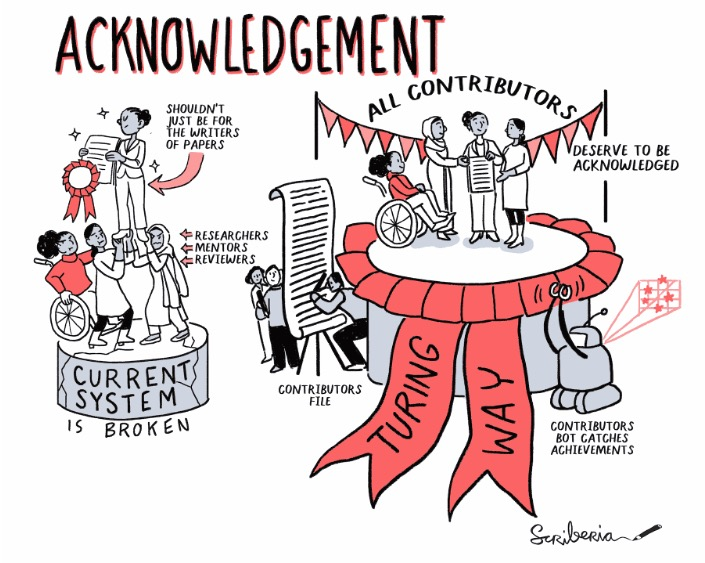
\includegraphics{open-results/figures/acknowledgement.jpg}

}

\caption{A hand drawn illustration shows that the traditional
acknowledgement system is broken then it shows how we try to acknowledge
them fairly. We have a contributors bot that catches all the
contributors information and stores them in contributors record}

\end{figure}

\emph{Figure 2: The process of acknowledging contributors in }The Turing
Way\emph{. \emph{The Turing Way} project illustration by Scriberia. Used
under a CC-BY 4.0 licence. DOI:
\href{https://doi.org/10.5281/zenodo.3332807}{10.5281/zenodo.3332807}.}

\hypertarget{contributor-guidelines}{%
\subsection{Contributor Guidelines}\label{contributor-guidelines}}

In addition to providing guidelines on how to assign authorship, you
also want to have a system in place to fairly recognize the
contributions of non-authoring contributors. Additionally, you may want
to consider guiding contributions to your results after they are made
open. Let's take a look at how you can go about this.

\hypertarget{crediting-non-authors-project-contributors}{%
\subsubsection{Crediting non-authors project
contributors}\label{crediting-non-authors-project-contributors}}

The CRediT taxonomy captures some of those ``non-author contributors''
roles such as funding acquisition and project administration, but there
is more to open results than scholarly outputs. This may include work
associated with maintenance, community management, data stewardship,
library and archiving, equity, diversity and inclusion efforts, funding,
project management, scientific event organisation, training activities
and more. We must ensure that there are processes in place to
acknowledge, value and reward this hidden labour {[}D'Ignazio, C., \&
Klein, L., 2020{]}.

You can consider adding a section to your authorship guidelines that
specifically talks about how you will acknowledge non-authors
contributors to different components of your open results.

\hypertarget{inviting-others-to-provide-feedback-and-contribute}{%
\subsubsection{Inviting others to provide feedback and
contribute}\label{inviting-others-to-provide-feedback-and-contribute}}

Often in academia, external feedback is not sought out until we submit
our manuscripts for publication to a journal or a conference in which
case 2-3 reviewers, presumably experts in the field, are recruited by an
editor to anonymously review your work. The process of peer review is a
much-dreaded one as the expectation tends to be the one that feedback
will set us back, keeping us from publishing our work, or attending a
conference.

But it does not have to be that way. Together, we can build a future in
which feedback from outside of those who are directly involved in the
project is sought out sooner and is welcomed with a much more positive
attitude. Of course, what you don't want is to get showered with
non-constructive opinions or personal attacks, which is why it is
important that you set the rules for contributions.

\textbf{Contributor guidelines} are documents that are often used in
open source projects to guide potential project contributors in
providing constructive feedback. They contain information about the
project itself, links to various parts of the project, and, most
importantly, a detailed description of \emph{how} to report errors
(often called ``bugs'' in code jargon), suggest changes, and even
request integration of large parts of code improving or adding features.

In the context of scientific research, the practice of having a document
that accompanies results and explicitly states how and what type of
feedback should be provided is not common. However, when you begin to
make more and more of your results open at different stages of your
research cycle, you may want to invite feedback to aspects of your work
that you think need it the most. You also may benefit from guiding the
way that feedback is received so that a) other people feel like it is
okay to contribute, and b) your corresponding author's email doesn't get
filled with non-constructive, not actionable and unclear advice.

Let's say, for example, that you and your team are drafting a research
manuscript and are getting pretty close to having all the information in
place for it to be shared as a preprint. This does not necessarily mean
that it is in a stage that you would consider ``final''---if such a
stage even exists!---but it contains enough information so that others
who are in the same or similar fields of research can understand what
the work is about and correctly interpret your results. This may be a
good time to solicit feedback from colleagues or the broader community,
and maybe even guide it towards aspects of your work that you think
would most benefit from review or contribution.

Maybe you want to drive the attention of your contributors to the
Methods section where a statistical analysis that is uncommonly used for
the kind of experiment you conducted is described. Or maybe you would
like some feedback from people with data visualization expertise so that
you can best present your data.

Where should you put your contributor guidelines? You may have one place
on your website where you can write general contributor guidelines to
any open result you and your team share and link to the guidelines in
your open result themselves. The contributor guidelines document can be
part of the authorship and contributorship document you prepared
following the tips in the previous section. You may even want to publish
a version of the record that has a permanent identifier so that the
links would never ``break''. Repositories such as GitLab/Github and
\href{https://zenodo.org/}{Zenodo} would allow you to post versions of
the original documents that would be linked to one another.

General contributor guidelines that also include the authorship
guidelines we talked about in the previous section may look something
like the sample template provided in `Assessment 1' at the end of this
lesson

\hypertarget{additional-resources-for-reference}{%
\subsubsection{Additional resources for
reference}\label{additional-resources-for-reference}}

\begin{itemize}
\item
  For additional tips on how to acknowledge contributors, check out
  \href{https://the-turing-way.netlify.app/community-handbook/acknowledgement.html}{Acknowledging
  Contributors The Turing Way}.
\item
  If working with online repositories such as GitHub, an app like
  `\href{https://allcontributors.org/}{all-contributors}' bot is a great
  way to automate capturing all kinds of contributions, from fixing bugs
  to organizing events to improving accessibility in the project.
\item
  More systematic work is being undertaken by
  \href{https://hidden-ref.org/}{hidden REF} who constructed a broad set
  of categories
  (\href{https://hidden-ref.org/categories/}{https://hidden-ref.org/categories})
  that can be used for celebrating everyone who contributes to the
  research.
\item
  There are several
  \href{https://the-turing-way.netlify.app/collaboration/research-infrastructure-roles.html}{research
  infrastructure roles} like community managers, data stewards, product
  managers, ethicists and science communicators, who are also being
  recognised as valued members in research projects with an intention to
  provide leadership paths for technical and subject matter experts,
  even when their contributions can't be assessed in tangible or
  traditional outputs
  {[}\href{https://the-turing-way.netlify.app/collaboration/research-infrastructure-roles.html}{reference}{]}.
\item
  The Declaration on Research Assessment (DORA)
  (\url{https://sfdora.org/}) is also a good resource to understand what
  researchers, institutions, funders and publishers can do to improve
  the ways in which researchers and the outputs of scholarly research
  are evaluated.
\end{itemize}

\hypertarget{how-to-ensure-your-open-results-are-properly-attributed-and-cited-by-others}{%
\section{How to ensure your open results are properly attributed and
cited by
others}\label{how-to-ensure-your-open-results-are-properly-attributed-and-cited-by-others}}

A citation is a reference to a source, which can include any of the
research objects described previously in this module, used in your
underlying research work. Citation (and other forms of acknowledgement)
have been the primary means by which researchers and scholars receive
credit for their work. Put differently, citations have largely been the
``reputation currency'' of science. In this section, we will discuss
various ways that you can ensure that your work is citable and that when
it is cited, you are properly credited.

\hypertarget{persistent-identifiers-pids}{%
\subsection{Persistent Identifiers
(PIDs)}\label{persistent-identifiers-pids}}

Persistent identifiers or PIDs are an invaluable part of the citation
process. They are long-lasting references to digital resources which
allow you to reliably find and verify resources leveraging underlying
metadata which is associated with the identifiers. More importantly, by
using PIDs, you can take advantage of scholarly systems that can help
you be more productive and efficient in sharing research outputs while
further supporting the acknowledgement of your research. Also, by using
PIDs you will be making your research findable, accessible,
interoperable, and reusable or FAIR, essentially machine-readable, and
responding to International and national efforts to open up science. The
best way to understand the value of PIDs though is to look at two
examples, ORCID iDs and DOIs (Digital Object Identifiers).

\hypertarget{orcids}{%
\subsection{ORCIDs}\label{orcids}}

ORCID iDs or ORCIDs are long-lasting unique identifiers for researchers.
\href{https://orcid.org/}{ORCID} is an acronym for `Open Researcher and
Contributor ID'. A freely available service for researchers, ORCID is
used globally. It is used to authenticate via a wide array of research
systems but it is also increasingly recommended and even required by
manuscript systems for preprints and journals
(\href{https://vimeo.com/495762735?embedded=true\&source=video_title\&owner=13723853}{introduction
video} by ORCID).

ORCIDs address the challenges around disambiguating author names and
distinguishing their works. So for instance, authors that share a common
name do not have to worry about their research being mixed up and not
associated with themselves. They are also useful towards supporting life
changes where your name can change but where your work can still be
associated via your ORCID. Of course, they also keep your data intact
even if you change your legal name at any time.

While you can use ORCID for your profile, it also facilitates
interoperability where entering your information once can save time on
entering it into other research information systems. ORCID supports an
array of research activities you are associated with from your roles and
grants to peer reviews you have done and data you have created. By
entering your ORCID and/or authenticating with other systems, they can
reuse this information so you do not have to enter it again, but you can
also have greater control over your record as well.

One way to demonstrate the benefit of interoperability via ORCID is by
enabling auto-updating with \href{https://www.crossref.org/}{Crossref}
(digital identifier service for primarily preprints and journals) and
\href{https://datacite.org/}{DataCite} (Digital identifier service for
data, software and other research objects). ORCID provides instructions
on how to enable auto-updates with these services so you do not have to
re-enter information from works and resources you have authored
{[}\href{https://support.orcid.org/hc/en-us/articles/360006896394-Auto-updates-time-saving-and-trust-building}{reference}{]}.
By enabling this feature, you will get notifications when new works are
connected with your profile and ready to be made public.

A good practice is to consistently use your ORCID and to provide ORCIDs
upfront in research projects, for instance, creating a contributors
resource (see
\href{https://the-turing-way.netlify.app/afterword/contributors-record.html}{this
example by The Turing Way}) where this information can be easily
accessed when resources are created over the life of a project (versus
always having to dig up this information in various places).

\hypertarget{digital-object-identifiers-dois}{%
\subsection{Digital Object Identifiers
(DOIs)}\label{digital-object-identifiers-dois}}

Digital Object Identifiers or DOIs are unique, persistent identifiers
provided for objects. The services mentioned above, Crossref and
DataCite, both use DOIs, where Crossref primarily is for works such as
journal articles, preprints, and book chapters, to name a few, while
DataCite has been mainly used for datasets, software, and presentations.
The two overlap in the types of research objects they cover, but
DataCite is used more often by repositories to provide DOIs and Crossref
is more widely used by publishers. Through these services, publishers
and repositories are committed at least to the persistence of the
overarching metadata about these objects and that links to them do not
break or rot. URLs or links used on the web are known to break, move, or
not be available while DOIs are intended to ensure that information
about the objects that they are linked to is not lost.

While one of the advantages of using DOIs is maintaining persistent
links to research objects that might normally be lost on project
websites, another advantage is that you can use the underlying metadata
associated with DOIs to help with certain tasks such as citing and
reporting your activities. One such service that demonstrates this value
is \href{https://citation.crosscite.org/}{CrossCite}. Enter a DOI,
choose a citation style and then format. What normally takes time
re-entering information and formatting took very little time. More and
more, scholarly services are leveraging DOIs to automate workflows and
help researchers reduce the amount of time it takes to do certain tasks
like the one described above, but of course, a system like this is
dependent on quality metadata and researchers using it.

Another advantage of using DOIs is that you can publish more aspects of
your research, beyond just a paper, from data and software to
presentations, and if done from the start, can be used to support the
transparency and replicability of your research. Not only does this
practice help towards recording how your research progressed, it can be
used to respond to open science recommendations and requirements, but it
is also just good scientific practice.

How can you use DOIs? One way to start and test how you can use DOIs is
via a \href{https://sandbox.zenodo.org/}{sandbox} service such as the
one Zenodo provides. Anything you do in the Zenodo sandbox is not
permanent and will be removed periodically. Once you are comfortable,
you can move to use the actual public \href{https://zenodo.org/}{Zenodo}
service or some of the other repositories listed at
\href{https://www.re3data.org/}{re3data}.

\hypertarget{all-the-pids}{%
\subsection{All the PIDs}\label{all-the-pids}}

There are a number of persistent identifiers beyond the two examples
above. A brief list can be found via
\href{https://project-thor.readme.io/docs/project-glossary}{Project
Thor} but absent are other identifiers such as
\href{https://ardc.edu.au/services/ardc-identifier-services/raid-research-activity-identifier-service/}{RAiDs}
(Research Activity Identifiers),
\href{https://scicrunch.org/resources}{RRID - Research Resource
Identification}, \href{https://ror.org/}{ROR ids (Research Organization
Registry)} and \href{https://www.igsn.org/}{IGSNs (International Generic
Sample Number Organization)}. Determining what identifiers to use can be
challenging but thankfully
\href{https://www.rd-alliance.org/national-pid-strategies-opportunities-collaboration-and-alignment}{national
PID strategies} are highlighting identifiers to focus on, at least to
start. ORCIDs for people. RORs for organisations. Crossref/DataCite DOIs
for research works/objects. RAiDs for research projects. Grant ID
(Crossref) for research funding.

\hypertarget{limitations}{%
\subsection{Limitations}\label{limitations}}

Not all the systems are ready for identifiers. For instance, identifiers
can be lost in research publications and it is best to provide
context/annotate them. In the case of journal articles, you can include
a bracketed description such as {[}Data set{]} or
\protect\hyperlink{software}{Software} with the citation and DOI in your
references section along with describing the identifiers used in
data/software availability or sharing sections. Also, it is important to
maintain consistency when using identifiers and citations so that it is
clear what other researchers should cite and credit. For example, use
the same citation/DOI on GitHub as compared to your website and in your
publications.

\hypertarget{self-assessment-1-develop-a-contributor-guideline-for-a-future-project-you-are-considering}{%
\section{Self-assessment \#1: Develop a contributor guideline for a
future project you are
considering}\label{self-assessment-1-develop-a-contributor-guideline-for-a-future-project-you-are-considering}}

\hypertarget{determining-authorship-and-acknowledging-project-contributors}{%
\subsection{Determining authorship and acknowledging project
contributors}\label{determining-authorship-and-acknowledging-project-contributors}}

Many examples and templates for creating contribution guidelines and
acknowledging contributors are available online. If you are starting a
project from scratch, read this chapter for\_
\href{https://the-turing-way.netlify.app/project-design/project-repo.html}{\emph{setting
up your project}}\emph{. You can directly clone/fork to start your repo
with this}
\href{https://github.com/alan-turing-institute/reproducible-project-template}{\emph{template
repository}} \_by making changes appropriate for your project.

Following the guidelines, the specific contributions of all author and
non-author contributors to a scientific work should always be outlined
in a project output or open results. Below we provide one way to
determine and attribute authorship. If your research team has previously
developed contribution guidelines, we recommend reusing them as your
team might be already familiar with them.

\hypertarget{template-for-adding-your-authorship-guidelines}{%
\subsection{TEMPLATE FOR ADDING YOUR AUTHORSHIP
GUIDELINES}\label{template-for-adding-your-authorship-guidelines}}

\begin{center}\rule{0.5\linewidth}{0.5pt}\end{center}

{[}HEADER{]}: Authorship guideline for {[}ADD PROJECT NAME{]}

Anyone who has contributed to the open results and is not already an
author will be acknowledged as a contributor in the acknowledgements
section of the open results.

\textbf{How to contribute to our open results}

\emph{Our team is committed to openly sharing our results with the
research community. We welcome contributions to our work in the form of
general feedback or specific suggestions on particular aspects of our
work.}

\emph{Open results for which we are seeking feedback are linked and
listed below:}

\begin{itemize}
\tightlist
\item
  New research proposal - Link to pre-registered proposal
\item
  Preprint - Link/persistent identifier (PID), like Digital Object
  Identifier (DOI) - particularly the methods section
\item
  Protocols - Link/PID to a protocols repository such as
  \href{https://protocols.io/}{\emph{protocols.io}}
\item
  Data - Link/PID
\item
  Source code - Link/PID
\end{itemize}

We welcome feedback that is positive or negative as long as it is
provided constructively. We would love to hear suggestions on how you
would address any issue you may identify with the work, with as much
clarity and examples as you may be able to provide.

Here are three ways you can provide us feedback:

\begin{enumerate}
\def\labelenumi{\arabic{enumi}.}
\tightlist
\item
  You can send us an email at {[}provide a team email{]}. In the body of
  your email please specify what result you are providing us feedback
  on, and be as specific as you can in referring to the part that you
  are talking about so that we are most likely to understand the
  feedback. We also welcome questions. We will not respond to your email
  if the content is an attack on the work or our team. Without your
  explicit consent, we will not share the content of your email
  associated with your name outside of our team.
\item
  You can publicly review our preprint by leaving a comment on the
  preprint server (if this option is available)\_
\item
  You can review our preprint on {[}add a link from the preprint server
  like\_ \href{https://prereview.org/}{\emph{PREreview.org}} or
  \href{https://arxiv.org/}{ArXiv}{]}, where your review can be opened
  and attributed with an ORCID iD.
\end{enumerate}

We thank you in advance for your time and willingness to help us improve
our work.

\textbf{What to expect after you contribute}

If your feedback came via email and is not an attack on our work or
team, we will make sure to reply to you in a timely manner---please give
our team up to 2 weeks to get back to you.

If you wrote a review on PREreview or on the comment section of the
preprint server, we would appreciate a quick email from you to let us
know of your contribution. All reasonable feedback and comments will be
addressed openly, or, if you prefer, we can reply via email.

If you give us consent either in the email or by posting your review
under your real name, we will acknowledge you and your feedback in the
next version of the open result.

If your feedback results in a substantial intellectual contribution to
the work, we will contact you to discuss opportunities for authorship in
the next version of the open result.

\begin{center}\rule{0.5\linewidth}{0.5pt}\end{center}

\hypertarget{assessment-2-a-case-study}{%
\section{Assessment \#2: A case study}\label{assessment-2-a-case-study}}

\begin{itemize}
\tightlist
\item
  Identify the contributors to each research object, at each stage in
  the research process.
\item
  Were these contributors credited? If so, was their contribution
  credited fairly with best practices from open science? If not, what
  could have been done differently?
\item
  Identify contributors that could have added value to different stages
  of your project and attribute their work fairly
\end{itemize}

\hypertarget{assessment-3-give-citations-for-the-research-objects-reused-in-your-work}{%
\section{Assessment \#3: Give citations for the Research Objects reused
in your
work}\label{assessment-3-give-citations-for-the-research-objects-reused-in-your-work}}

Generate a citation from a DOI associated with a dataset that you
preserved in a repository, like, Zenodo, using the crosscite tool. Don't
have a dataset DOI, note this for your future research. In the meantime,
find a DOI for another one of your research objects, like a paper, and
generate a citation using CrossCite.

\hypertarget{references-8}{%
\section{References}\label{references-8}}

\begin{itemize}
\tightlist
\item
  Fleming, N. (2021). The authorship rows that sour scientific
  collaborations. In Nature (Vol. 594, Issue 7863, pp.~459--462).
  Springer Science and Business Media LLC.
  \url{https://doi.org/10.1038/d41586-021-01574-y}
\item
  D'Ignazio, C., \& Klein, L. (2020). 7. Show Your Work. In Data
  Feminism. Retrieved from
  \url{https://data-feminism.mitpress.mit.edu/pub/0vgzaln4}
\item
  ``PREreview. Catalyzing change in peer review through equity,
  openness, and collaboration'' \url{https://prereview.org/}.
\item
  ``Auto-updates: time-saving and trust-building.'' ORCID,
  \url{https://support.orcid.org/hc/en-us/articles/360006896394-Auto-updates-time-saving-and-trust-building}
\item
  The Turing Way Chapters: Project Ownership; Tips for Getting
  Authorship Right and Acknowledging Contributors; Research
  Infrastructure Roles; Creating project repositories.
  \url{https://the-turing-way.netlify.app/welcome.html}, The Turing Way
  Community, Zenodo, 27 July 2022, doi:10.5281/zenodo.6909298.
\item
  ``ICMJE \textbar{} Recommendations \textbar{} Defining the Role of
  Authors and Contributors.'',
  \href{http://www.icmje.org/recommendations/browse/roles-and-responsibilities/defining-the-role-of-authors-and-contributors.html}{www.icmje.org/recommendations/browse/roles-and-responsibilities/defining-the-role-of-authors-and-contributors.html}.
\item
  Colbert, Melissa C., Robert B. Nussenblatt, and Michael M. Gottesman.
  ``Integrity in Research: Principles for the Conduct of Research.''
  Principles and Practice of Clinical Research. Academic Press, 2018.
  33-46.
\end{itemize}

\hypertarget{opensciency-open-results-authors}{%
\chapter{OpenSciency Open Results:
Authors}\label{opensciency-open-results-authors}}

\textbf{Batalha, Natasha}

NASA Ames Research Center

\url{https://orcid.org/0000-0003-1240-6844}

\url{https://github.com/natashabatalha}

\url{https://twitter.com/natashabatalha}

\textbf{Camacho Toro, Reina}

CERN/CNRS, LA-CoNGA physics

\url{https://orcid.org/0000-0002-9192-8028}

\url{https://github.com/camachoreina}

\url{https://twitter.com/rcamachotoro}

\textbf{Campitelli, Elio}

University of Buenos Aires

\url{https://orcid.org/0000-0002-7742-9230}

\url{https://github.com/eliocamp}

\url{https://twitter.com/d_olivaw}

\textbf{Dunleavy, Daniel}

Florida State University

\url{https://orcid.org/0000-0002-3597-7714}

\url{https://github.com/dunldj}

\url{https://twitter.com/Dunleavy_Daniel}

\textbf{Erdmann, Christopher}

Michael J. Fox Foundation

\url{https://orcid.org/0000-0003-2554-180X}

\url{https://github.com/libcce}

\url{https://twitter.com/libcce}

\textbf{Fouilloux, Anne}

University of Oslo, Norway

\url{https://orcid.org/0000-0002-1784-2920}

\url{https://github.com/annefou}

\textbf{Lacerda, Michel}

Georgia Institute of Technology

\url{https://orcid.org/0000-0002-8433-6964}

\url{https://github.com/michelusp}

\textbf{Saderi, Daniela}

PREreview, Code for Science \& Society

\href{}{https://orcid.org/0000-0002-6109-0367}

\url{https://github.com/dasaderi}

\url{https://twitter.com/Neurosarda}

\textbf{Sharan, Malvika}

The Alan Turing Institute and Open Life Sciences

\url{https://orcid.org/0000-0001-6619-7369}

\url{https://github.com/malvikasharan}

\url{https://twitter.com/malvikasharan}

\part{Open Science tools}

\begin{itemize}
\tightlist
\item
  Definition: What do we mean by ``Open Science tools''?
\item
  What's the difference between `open' and `closed' tools? Why use Open
  Science tools?
\item
  How do Open Science tools fit into the research lifecycle?
\item
  How do Open Science tools address responsible practices?
\end{itemize}

\hypertarget{introduction-to-open-science-tools.}{%
\section*{Introduction to Open Science
tools.}\label{introduction-to-open-science-tools.}}
\addcontentsline{toc}{section}{Introduction to Open Science tools.}

\markright{Introduction to Open Science tools.}

\emph{(What are Open Science tools? Why use Open Science tools? How do
Open Science tools fit into the research lifecycle?)}

This lesson is the first of OpenCore Module 5: Open Science Tools and
Resources. This Module provides a collection of tools that are available
to increase the visibility and discoverability of your project. It
complements the previous OpenCore Modules (Ethos of Open Science, Open
Data, Open Software, and Open Results) by enhancing the practical
implementation of the Open Science concepts explained previously. While
earlier modules focused on the concepts, advantages, and disadvantages
of responsible Open Science practices, this module will focus more on
the practical applications of responsible Open Science practices. We
focus on a few key tools, and highlight how they fit across the research
lifecycle.

In this first lesson, you will be introduced to the \_What \_and the
\emph{Why} of Open Science tools. First, we provide a definition of Open
Science tools. Second, we discuss the differences between `open' and
`closed' tools and highlight the advantages of using open tools. Third,
we elaborate on the research lifecycle, and show how Open Science tools
fit into a researcher's project workflow.

\hypertarget{what-do-we-mean-by-open-science-tools}{%
\section*{What do we mean by ``Open Science
tools''?}\label{what-do-we-mean-by-open-science-tools}}
\addcontentsline{toc}{section}{What do we mean by ``Open Science
tools''?}

\markright{What do we mean by ``Open Science tools''?}

We use the word ``tools'' to cover any type of resource or instrument
that can be used to support your research. In this sense, tools can be a
collection of useful resources that you might consult during your
research, a software that you could use to create and manage your data,
or even a human infrastructure, such as a community network that you
could join to get more guidance and support on specific matters.

In this context, Open Science tools are any tools that enable and
facilitate openness in research, and support responsible Open Science
practices. It is important to note that Open Science tools are very
often open source and/or free, but not necessarily.

\hypertarget{whats-the-difference-between-open-tools-and-closed-tools-why-use-open-science-tools}{%
\section*{What's the difference between `open' tools and `closed' tools?
Why use Open Science
tools?}\label{whats-the-difference-between-open-tools-and-closed-tools-why-use-open-science-tools}}
\addcontentsline{toc}{section}{What's the difference between `open'
tools and `closed' tools? Why use Open Science tools?}

\markright{What's the difference between `open' tools and `closed'
tools? Why use Open Science tools?}

One can intuitively grasp the difference between open and closed in
relation to the ``tools'', thinking of openness in terms of exchange
with the environment. One should bear in mind that it is not a black and
white separation, but rather a spectrum of options.

When speaking of useful resources that you can \emph{re-use} - such as
text, visuals, audio, video - it is important to pay attention to the
license on the possibilities and conditions for re-use. Lack of
indication of a license leads to impossibility to re-use the material.
As indicated in 🔗 Module 1 Ethos of Open Science, Lesson 5🔗,
\href{https://creativecommons.org/}{Creative Commons licenses} is one of
the most common set of open licenses given to written content of any
kind, allowing re-use and requiring attribution, with a spectrum of
openness, from least to most open (or CC0, equivalent to public domain).

Software can be proprietary (``closed'') or open source. It is called
open source when the original source code is made freely available and
may be redistributed and modified. Generally, software has a separate
set of licenses designed specifically for code projects that covers both
the open distribution of the code itself as well as executable versions
of the program which non-programmers can run. More information and
details on open software can be found in the 🔗Open Software Module🔗.

Human infrastructure refers to a network of relationships between
stakeholders interested in the conduct and outcomes of responsible Open
Science (more on those stakeholders can be found in 🔗Module 1, Lesson
3🔗). Communities -- or groups of people who share a geographical
location, affiliation, common interest, or practice -- play a key role
in the human infrastructure aspect of open science. As everything else,
communities can vary in their degree of openness. A community can take
the form of a mailing list, conference, meet-up or messaging app as a
way to stay in touch. In that case, being open would imply that anyone
could join the community and be welcomed to speak, decisions would be
made transparent, and communications are largely public. On the other
hand, a closed community implies that membership is restricted by
invitation and/or a fee, resources and communications are not public,
and decision processes are not necessarily transparent. More ideas on
how to increase participation of stakeholders and how to build and lead
inclusive communities can be found in 🔗Module 1, Lesson 3🔗 and 🔗this
module, Lesson 4🔗.

\hypertarget{activityexercise-1}{%
\subsection*{Activity/exercise}\label{activityexercise-1}}
\addcontentsline{toc}{subsection}{Activity/exercise}

Now let's practice by looking at some typical case studies and
solutions, reflecting on the benefits and obstacles of open and closed
tools.

\textbf{Case study \#1: Closed vs open resources}

\textbf{Case study \#2: Closed vs open software}

You are a researcher who has been using a proprietary MATLAB platform to
analyze data and create models. You are getting a new job, at a
different institution. Unfortunately, the new workplace does not have a
license for MATLAB, therefore you cannot access your own code and data,
stored in the proprietary file formats, and moreover, cannot continue
your routine workflow with analysis. What are your options now?

\begin{itemize}
\tightlist
\item
  You can purchase individual license for this proprietary software, or
  persuade the institute to purchase a group or campus-wide license
\item
  You could consider using open source alternatives for programming and
  numerical computing, such as GNU Octave, Sage, or even Python
  programming language and its scientific packages. It would not only
  save you money now, but provide the continuity of the tool - if you
  move again, to a different institution.
\end{itemize}

\textbf{Case study \#3: Closed vs open communities}

\begin{itemize}
\tightlist
\item
  \textbf{Example:}
\end{itemize}

Open science tools provide numerous benefits, many of which have been
discussed in the previous modules. For example, they can help you
collaborate openly and share easily; organize and manage your work;
track how your work is treated and shared; and follow leading
responsible Open Science practices.

Open Science practices enable easier access to existing tools and
resources that promote collaboration between professionals with similar
interests and research objects. For example, someone in Asia wanting to
study Central African rainforest species could visit an online species
database made available by other scientists. Despite their physical
distance, many reasons lead to inequality in access to scientific
resources, from institutional barriers to paid content.

There are efficient and coordinated ways to share resources in general.
One of them is using {📖}version control {📖}, which is a system to keep
track of any changes made to one or more files over time. That also
serves as a backup for your work.You might have already done that -- for
example, if you ever used Google Docs. It stores a version of your work
as you type it, and you can invite other users to work collaboratively
in the same document, keeping record of all changes made by all users.

One broadly used tool for version control is Git. It enables version
control either online or on the user's machine {[}see
\url{https://git-scm.com/}{]}. Related services include GitHub, Gitlab,
and Bitbucket. Information is stored in online repositories where people
can clone, edit, and review each other's content.

Another way to share your work is by using standardized
{📖}workflows{📖}. A standardized workflow is typically a sequence of
steps commonly used for a given purpose, such as accessing and
manipulating genomic data. A good open science practice, then, is to
share those workflows in platforms such as
\url{https://galaxyproject.org/} -- which allows any user to replay
those steps right there for free, quickly and easily. That and other
similar services enable you to show a step-by-step overview of what
other researchers did, build on their work, and share your new ideas.

Including {📖}metadata{📖}, the data that describes your data, can
significantly enhance the findability of your research object. Some
examples of metadata are the keywords associated with a publication, the
time range and instrument name of a given observational data set, and
the ORCID number for a given person. Metadata is a tool that search
interfaces use to more quickly find a resource. In fact, Google uses a
metadata language called `Schema.org' to build its search algorithm (see
\url{https://schema.org/} for more information).

Many research fields have their own metadata standards (e.g.~SPASE for
space physics: \url{https://spase-group.org/data/}), but remember that
each website you use has something similar behind that magnifying glass
button. Taking the extra time to include some basic descriptors for your
research object can make your contribution to your research field much
more findable. The same way finding someone else's work on the Internet
might help you, making your own work more discoverable is a great
contribution to Open Science!

Next, we'll highlight how open science tools and resources fit in the
research lifecycle.

\hypertarget{how-do-open-science-tools-fit-into-the-research-lifecycle}{%
\section*{How do Open Science tools fit into the research
lifecycle?}\label{how-do-open-science-tools-fit-into-the-research-lifecycle}}
\addcontentsline{toc}{section}{How do Open Science tools fit into the
research lifecycle?}

\markright{How do Open Science tools fit into the research lifecycle?}

The complex nature of research in the modern scientific community --
involving multiple stages, steps, contributors, and stakeholders in the
process -- benefits from certain frameworks and definitions to
structure, organize, and somewhat standardize the research process for
the sake of responsible and reproducible practices.

The 🔗Open Results🔗 module introduced you to the definitions and nine
stages of the research lifecycle and workflow. Let's define these terms
again.

\begin{itemize}
\tightlist
\item
  Research framework
\item
  Research workflow
\item
  Research lifecycle
\end{itemize}

There is quite some theory behind the models for research frameworks,
lifecycles, and workflows (REF), including linear, circular, multi-loop,
and multi-step flows. For the sake of clarity and pragmatism of mapping
the Open Science tools used within the research lifecycle, we will
consider a concise 6-stage spiraling model for the research workflow,
covering \textbf{discovery, analysis,} and \textbf{writing} as well as
\textbf{publication}, \textbf{outreach}, and \textbf{assessment} (see
Fig.)

Ref:\url{https://figshare.com/articles/presentation/Of_Shapes_and_Style_visualising_innovations_in_scholarly_communication/3468641}

Most steps of the research workflow are supported by online applications
(Kramer and Bosman, 2016). These digital (Open Science) tools have
actually influenced the way in which we perform and share research,
opening it up to a global audience.

Open Science tools can be used for

\begin{itemize}
\tightlist
\item
  Discovery: Tools for finding content to use in your research
\item
  Analysis: Tools to process your research output, e.g.~tools for data
  analysis and visualization
\item
  Writing: Tools to produce content, such as Data Management Plans,
  presentations, and pre-prints
\item
  Publications: Tools to use for sharing and/or archiving research
\item
  Outreach: Tools to promote your research
\end{itemize}

The usage of such tools by researchers across different disciplines has
been surveyed and reviewed in several efforts (Kramer and Bosman, 2016,
Bezuidenhout and Havemann, 2021). Numerous digital tools have been
mapped on the ``discovery, analysis and writing, publication, outreach,
and assessment'' stages of the research lifecycle (see Fig). As we saw
in the previous section, all tools have varying degrees of openness.
Purposefully choosing tools to use at each stage to increase
transparency, findability, and reproducibility, you are able to
construct and define your research workflow in alignment with
responsible Open Science practices. As was discussed in Module 1, Ethos
of Open Science, open should not be a thoughtless default or
afterthought, but included into the design and inception of the research
project. Your choice of Open Science tools can be individual, but most
often it would benefit from group discussions within your research team,
institution, and communities of practice.

Note: the concepts of workflow and lifecycle are widely used and applied
to parts of the research, e.g.~data. Data workflow, data lifecycle are
discussed in depth in 🔗Lesson X of the Module Open Data🔗.

\hypertarget{how-do-open-science-tools-address-responsible-practices}{%
\section*{How do Open Science tools address responsible
practices?}\label{how-do-open-science-tools-address-responsible-practices}}
\addcontentsline{toc}{section}{How do Open Science tools address
responsible practices?}

\markright{How do Open Science tools address responsible practices?}

The 🔗Open Data and Open Results🔗Modules introduced the concept of FAIR
principles and discussed how their application according to best
practices can increase the visibility and uptake of our research.

Let's refresh the terms:

\begin{itemize}
\tightlist
\item
  \textbf{FAIR Data Principles} - Findable, Accessible, Interoperable,
  \& Reusable. \href{https://doi.org/10.1038/sdata.2016.18}{Wilkinson et
  al.~(2016)} provided FAIR Guiding Principles for scientific data
  management and stewardship;
  \href{https://doi.org/10.15497/RDA00068}{Hong et al.~(2022)} establish
  FAIR principles for research software.
\item
  \textbf{CARE Principles} - Collective Benefit, Authority to Control,
  Responsibility, \& Ethics.
  \href{http://doi.org/10.5334/dsj-2020-043}{Carroll et al.~(2020)}
  established the CARE Principles for Indigenous Data Governance,
  complementing the FAIR data principles.
\end{itemize}

Best practices to implement these principles include describing data
using metadata standards and controlled vocabularies, assigning
licenses, and uploading data to repositories that allow for creation of
``📖{persistent identifiers📖}''. Examples of useful Open Science tools
include:

\begin{itemize}
\tightlist
\item
  Data Management Plan (DMP) tool, which allows you to create and share
  your data management plans to meet funder requirements and as a best
  practice for managing your data (link to website, to Lessons)
\item
  Data Repositories, which assign persistent identifiers to your data
  (example or link)
\item
  Tools for integration research management with DMPtool and
  repositories (example or link)
\item
  Communities - national and international, discipline-specific, or open
  science-centered - can be of incredible value in curating resources
  and building communities of practice for researchers and other
  stakeholders in adopting FAIR principles. Examples include the FAIR
  Data Forum \url{https://fairdataforum.org/} and the Research Data
  Alliance (RDA) \url{https://www.rd-alliance.org/}
\end{itemize}

Working within the ethos of the FAIR and CARE principles can help to
ensure that research is accessible, inclusive, ethical, and responsible.
More about FAIR principles and practical steps to make your data FAIR
can be found here: \url{https://www.go-fair.org/fair-principles/}

\hypertarget{self-assessment-questions-for-reflection}{%
\section*{Self-Assessment: Questions for
reflection:}\label{self-assessment-questions-for-reflection}}
\addcontentsline{toc}{section}{Self-Assessment: Questions for
reflection:}

\markright{Self-Assessment: Questions for reflection:}

\begin{enumerate}
\def\labelenumi{\arabic{enumi}.}
\tightlist
\item
  Assessment of your (open science) tools and resources
\end{enumerate}

Most probably you are already using some tools and resources, even if
you are new to open science practices. Here we invite you make a
preliminary revision of them:

\begin{itemize}
\tightlist
\item
  Think of all the tools and resources you use in your
  study/research/work and rely on - resources (content with text/media),
  software and communities. Think of all stages of your research -
  discovery, analysis, writing, publication, outreach and assessment.
\item
  Tools have varying degrees of openness, dictated by various factors.
  Imagine (or draw) the scale from 0 to 10, where 0 stands for
  completely closed and 10 for completely open.
\item
  For which of the tools (from categories of resources, software and
  communities) place it on the scale on a number that reflects the
  degree of openness.
\item
  How many tools do fall towards the lower part of the scale (0 to 4)?
  Take a moment to reflect if these tools are in line with your actual
  preference, goals and necessities in the long-term run.
\item
  Perform a quick search using search engine or this open dataset of
  Open Science tools (https://kumu.io/access2perspectives/dost\#dataset)
  for more open alternatives (e.g.~free, open source) and jot them down
  ``for your information''.
\end{itemize}

In the next lessons we will introduce you to various tools, which you
may not have heard yet. Stay tuned!

\hypertarget{open-science-tools-across-the-research-lifecycle}{%
\chapter{Open Science tools across the research
lifecycle}\label{open-science-tools-across-the-research-lifecycle}}

\begin{itemize}
\tightlist
\item
  Open Science tools for protocols
\item
  Open Science tools for data

  \begin{itemize}
  \tightlist
  \item
    Tools for Data Management Plans
  \item
    Sharing data with your (research) team
  \item
    Data repositories
  \end{itemize}
\item
  Open Science tools for code

  \begin{itemize}
  \tightlist
  \item
    Collaborative development tools
  \item
    Code repositories
  \end{itemize}
\item
  Open Science tools for results
\item
  Open Science tools for authoring

  \begin{itemize}
  \tightlist
  \item
    Collaborative writing tools
  \item
    Reference management tools
  \item
    Publishing Open Science and Open Access
  \end{itemize}
\end{itemize}

\hypertarget{open-science-tools-across-the-research-lifecycle-1}{%
\section{Open Science Tools across the Research
Lifecycle}\label{open-science-tools-across-the-research-lifecycle-1}}

In the first lesson, we briefly defined Open Science tools,
distinguished open from closed tools, and highlighted the advantages of
Open Science tools. We also gave a brief introduction to the Research
Lifecycle, and discussed how open tools fit in this workflow. In this
second lesson, we'll highlight a few key tools for each aspect of the
research lifecycle.

In this module, we'll focus on the following elements of the project
workflow rather than distinct research stages, because many tools
support more than one stage. We will cover tools specifically for
protocols; data; code; results; and authoring. We'll only highlight a
few tools; more tools and resources are currently available than we
could possibly list (see Figure below).

Ref:
\url{http://46eybw2v1nh52oe80d3bi91u-wpengine.netdna-ssl.com/wp-content/uploads/2021/12/Data-and-AI-Landscape-2021-v3-small.jpg}

\hypertarget{open-science-tools-for-protocols}{%
\subsection{Open Science tools for
protocols}\label{open-science-tools-for-protocols}}

In the last decades, we have seen an avalanche of development of the
tools for management of research projects and laboratories, which
address the ever-increasing need for speed, innovation, and
transparency. Such tools are developed to support collaboration, ensure
data integrity, automate processes, create workflows and increase
productivity.

Some research groups have been adapting commonly used project management
tools for their own team needs, such as Trello, a cloud-based online
tool. Such software facilitates sharing materials within the group and
managing projects and tasks, while allowing space for some
customization.

Platforms and tools, which are finely tuned to meet researchers' needs
(and frustrations), have appeared as well, often founded by scientists -
for scientists. To give you a few examples, let's turn to experimental
science. A commonly used term and research output is{📖} protocol{📖}.

Protocol can be defined as ``A predefined written procedural method in
the design and implementation of experiments. Protocols are written
whenever it is desirable to standardize a laboratory method to ensure
successful replication of results by others in the same laboratory or by
other laboratories.'' (REF According to the University of Delaware (USA)
Research Guide for Biological Sciences)

In a broader sense, protocol also comprises documented computational
workflows, operational procedures with step-by-step instructions, or
even safety checklists.

\textbf{Protocols.io}
(\href{https://www.protocols.io/}{https://www.protocols.io/)} is an
online and secure platform for scientists affiliated with academia,
industry and non-profit organizations and agencies. It allows them to
create, manage, exchange, improve, and share research methods and
protocols across different disciplines. This resource is useful for
improving collaboration and recordkeeping, increasing team productivity,
and even facilitating teaching, especially in the life sciences. In its
free version, protocols.io supports publicly shared protocols, while
paid plans enable private sharing, e.g.~for industry.

Some of the tools are specifically designed for open science with an
open by design idea straight from the beginning, and aim to support the
research lifecycle at all stages, and allow for integration with other
open science tools.

Most prominent one includes \textbf{Open Science Framework (OSF)},
developed by Center for Open Science (link). OSF is a free and open
source project management tool that supports researchers throughout
their entire project lifecycle through open, centralized workflows. It
captures different aspects and products of the research lifecycle,
including developing a research idea, designing a study, storing and
analyzing collected data, and writing and publishing reports or
papers.''

OSF is designed to be a collaborative platform where users can share
research objects from several phases of a project. It serves as support
for a broad and diverse audience, including researchers that might not
have been able to access so many resources due to historic socioeconomic
disadvantages. OSF also contains other tools in its own platform:

\begin{verbatim}
“While there are many features built into the OSF, the platform also allows third-party add-ons or integrations that strengthen the functionality and collaborative nature of the OSF. These add-ons fall into two categories: citation management integrations and storage integrations. Mendeley and Zotero can be integrated to support citation management, while Amazon S3, Box, Dataverse, Dropbox, figshare, GitHub, and oneCloud can be integrated to support storage. The OSF provides unlimited storage for projects, but individual files are limited to 5 gigabytes (GB) each.”
\end{verbatim}

(maybe a note on preregistration offered by OSF, which can be powerful)

\hypertarget{open-science-tools-for-data}{%
\section{Open Science tools for
data}\label{open-science-tools-for-data}}

``Research data means any information, facts or observations that have
been collected, recorded or used during the research process for the
purpose of substantiating research findings. Research data may exist in
digital, analogue or combined forms and such data may be numerical,
descriptive or visual, raw or processed, analyzed or unanalyzed,
experimental, observational or machine generated. Examples of research
data include: documents, spreadsheets, audio and video recordings,
transcripts, databases, images, field notebooks, diaries, process
journals, artworks, compositions, laboratory notebooks, algorithms,
scripts, survey responses and questionnaires.'' Ref:
\url{https://policy.unimelb.edu.au/MPF1242\#section-5}

Data is the one type of research object that is universal. Sharing your
datasets publicly allows other researchers (and you!) direct access to
the data to allow further study.

\hypertarget{tools-for-data-management-plans}{%
\subsection{Tools for Data Management
Plans}\label{tools-for-data-management-plans}}

Every major research foundation and federal government agency now
requires scientists to file a data management plan (DMP) along with
their proposed research plan. Data as research in its whole, and as
other elements (code, publication) have their own lifecycle and
workflow, which needs to be in the plan. DMPs are a critical aspect of
Open Science and they help keep other researchers informed and on track
throughout the data management lifecycle. DMPs that are successful
typically include a clear terminology about FAIR and CARE and how they
will and are applied.

The data management lifecycle is typically circular. Research data are
valuable and reusable long after the project's financial support ends.
Data reuse can extend beyond our own lifetimes. Therefore, when
designing a project or supporting an existing corpus of data, we need to
remain cognizant of what happens to the data after our own research
interaction ends.

There are a few Open Science resources available to get you started and
to keep you on track. The \emph{DMPTool https://dmptool.org/} in the US
helps researchers by using a template which lists each funder's
requirements for specific directorate requests for proposals (RFP). The
DMPTool also publishes other open DMP from funded projects which can be
used for improving your own DMP. The Research Data Management Organizer
(RDMO) enables German institutions as well as researchers to plan and
carry out their management of research data. ARGOS is used to plan
Research Data Management activities of European and nationally funded
projects (e.g.~Horizon Europe, CHIST-ERA, the Portuguese Foundation for
Science and Technology - FCT). ARGOS produces and publishes FAIR and
machine actionable DMPs that contain links to other outputs,
e.g.~publications-data-software, and minimizes the effort to create DMPs
from scratch by introducing automations in the writing process. OpenAIRE
provides a guide on how to create DMP.

\hypertarget{sharing-data-with-your-research-team}{%
\section{Sharing data with your (research)
team}\label{sharing-data-with-your-research-team}}

\hypertarget{data-repositories}{%
\subsection{Data repositories}\label{data-repositories}}

Originally data repositories appeared in different disciplines of
research around the needs of research communities and dataset types,
such as \emph{Protein Data Dank }(PDB) \url{https://www.rcsb.org/} for
3D structures of proteins and nucleic acids, or \emph{Genbank} - NIH
genetic sequence database, containing annotated publicly available
nucleic acid sequences. Another example is a public repository of
microscopy bio-image datasets from published studies, \emph{The Image
Data Resource} (IDR) (ref). \_The Electron Microscopy Public Image
Archive (\_EMPIAR) \url{https://www.ebi.ac.uk/empiar/}, is a public
resource for raw cryo-EM images. \emph{OpenNeuro}
\url{https://openneuro.org/} is a open platform for validating and
sharing brain imaging data. These tools enable easy access, search, and
analysis of these annotated datasets.

As noted in Lesson 2, open science tools such as data repositories
should ensure the guidelines for FAIR data, mainly attribution of
persistent identifies (e.g.~DOI), metadata annotation,
machine-readability.

Data repositories that include FAIR principles and work across borders
and disciplines include \emph{Zenodo} (\url{https://zenodo.org/}),
funded by the European OpenAire project and hosted by CERN. It is
probably one of the most known and widely used, as it has an easy
interface, support of community curation, and allows depositing diverse
types of research outputs - from datasets and reports to publications,
software, multimedia content.

The main drawback for this choice is that Zenodo is relatively lacking
in documentation and metadata; a dataset stored on this site is not as
easily findable or visible to the community compared to storing the data
at a domain-specific repository (e.g.~EarthData:
\url{https://www.earthdata.nasa.gov/}, BCO-DMO for marine ecosystem
research data, or Environmental Data Initiative for environmental or
ecological data), or a cross-domain repository (e.g.~DataOne:
\url{https://www.dataone.org/}).

Noted exceptions to this rule include communities hosted on Zenodo that
curate their materials to enhance findability (e.g.~Open Science
Community Saudi Arabia (OSCSA):
\url{https://zenodo.org/communities/1231231664/?page=1\&size=20}, Turing
Way community:
\url{https://zenodo.org/communities/the-turing-way/?page=1\&size=20}).
More on the role and power of communities will be covered in Lesson X
(communities).

Another example of a non-profit data repository is \emph{Dataverse}
\url{https://dataverse.org/}, hosted by Harvard University. The
Dataverse Project is an open source online application to share,
preserve, cite, explore, and analyze research data, available to
researchers of all disciplines worldwide for free.

\emph{The Dryad Digital Repository} \url{https://datadryad.org/} is a
curated online resource that makes research data discoverable, freely
reusable, and citable. Unlike previously mentioned tools, it operates on
a membership scheme for organizations such as research institutions and
publishers.

\emph{Datacite }\url{https://datacite.org/} is another global non-profit
organization that provides DOIs for research data and other research
outputs, on a membership basis.

Data services and resources for supporting research require robust
infrastructure which relies on collaboration. Some examples of
initiatives on the infrastructures of data services include The EUDAT
Collaborative Data Infrastructure (or EUDAT CDI)
\url{https://www.eudat.eu/}, sustained a network of more than 20
European research organizations,

Private companies as well host and maintain online tools for sharing
research data and files. \emph{Figshare} \url{https://figshare.com/} is
one of the examples of a free and open access service, giving a DOI for
all types of files and recently developing a restricted publishing model
to accommodate intellectual property (IP) rights requirements. It allows
sharing the outputs only within a customized Figshare group (could be
your research team) or with users in a specific IP range. Additional
advances include integration with code repositories, such as GitHub,
GitLab, and Bitbucket.

\emph{GitHub} \url{https://github.com/}, owned by Microsoft, is often
the default data repository for coders. It allows collaborative work,
version control, project management, and is widely used by researchers
for uploading datasets, files, notes, hosting simple static webpages to
showcase their achievements. Github does not give you a DOI, but allows
you to state the license for re-use and ways to cite your work.

Much more research data repositories could be found in the publicly open
Registry of Research Data Repositories \url{https://www.re3data.org/}.
OpenAire-hosted search engine
\url{https://explore.openaire.eu/search/find/dataproviders} provides a
powerful search function of data and repositories, with country, type,
thematic and others filters, and enables downloading of the data.

Caution: Amount of data, repositories and different policies can be
overwhelming. When in doubt, which repository is for you, make sure you
consult librarians, data managers and/or data stewards in your
institution, or check within your discipline-specific or other community
of practice.

\hypertarget{open-science-tools-for-code}{%
\subsection{Open Science tools for
code}\label{open-science-tools-for-code}}

If your project involves coding, such as custom analysis code, you can
share it or collaborate using tools such as Jupyter Notebooks. These
notebooks can be shared with a variety of permissions on JupyterLab,
Google Colab, and similar websites. For a more permanent solution, you
can use containerized environments to share the entire analysis
environment, which includes the installed software packages, the data
used, all custom analysis and plotting routines, and even the
publication draft. A few examples of containerized environment services
are DeepNote and Binder (DeepNote: \url{https://deepnote.com/}, Binder:
\url{https://mybinder.org/}).

\hypertarget{collaborative-development-tools}{%
\subsection{Collaborative development
tools}\label{collaborative-development-tools}}

\hypertarget{code-repositories}{%
\subsubsection{Code repositories}\label{code-repositories}}

\begin{itemize}
\tightlist
\item
  Github
\item
  GitLab
\item
  BitBucket
\item
  SourceForge
\end{itemize}

\hypertarget{open-science-tools-for-results}{%
\subsection{Open Science tools for
results}\label{open-science-tools-for-results}}

\begin{itemize}
\tightlist
\item
  Visual tools for graphs, dataviz, sharing
\end{itemize}

\hypertarget{open-science-tools-for-authoring}{%
\subsection{Open Science tools for
authoring}\label{open-science-tools-for-authoring}}

\hypertarget{collaborative-writing-tools}{%
\subsubsection{Collaborative writing
tools}\label{collaborative-writing-tools}}

One of the commonly used processes in research is creation and editing
of documents, such as meeting notes, conference abstracts, manuscripts,
checklists etc.

Collaborative editing process has become really easy with online tools
like Google Docs, Bit AI and others, because of their easy interface and
version history. However, these tools are proprietary, so not fully
open.

Open-source, web-based collaborative tools for editing include tools
such as Etherpad \url{https://etherpad.org/}, HackMD
\url{https://hackmd.io/} and HedgeDoc \url{https://hedgedoc.org/}
(formerly known as CodiMD). These editors use a Markdown language,
lightweight markup language, for creating formatted text for the web. It
has a simple syntax, and therefore allows more users to be engaged and
focus on content, including graphics, tables, lists. Moreover, Markdown
is useful when creating documentation in GitHub, as we discussed in the
previous sections, commonly used data and code repository and
collaboration space.

LaTex / TeX markup language provides a steeper learning curve, but
allows much more nuanced features for scientific and technical
documentation, such as formatting of books, articles, mathematical
formulas etc. Collaborative online tool utilizing LaTex is called
Overleaf \url{https://overleaf.com/}, and it is widely used in the
research community to share and edit LaTex files.

\hypertarget{reference-management-tools}{%
\subsubsection{Reference management
tools}\label{reference-management-tools}}

At the \emph{Discovery} and \emph{Publication} stages of the research
lifecycle reference management tools are particularly useful to search
for publications, collect and organize them, annotate, cite, and share.
Such tools should facilitate your research workflow by easy
addition/import of references, bibliography construction, adaptation to
various citation styles requested by different journals/publishing
houses.

\_EndNote \_is a citation manager tool owned by Clarivate Analytics.
However, it is proprietary software and not free for researchers (closed
tool), so it is beyond our interest.

\emph{Mendeley} \url{https://www.mendeley.com/} - now owned by publisher
Elsevier, is a free software with very similar functionality.

\emph{Zotero} \url{https://www.zotero.org/} is an open-source and
independent organization-hosted online tool.

Both Zotero and Mendeley tools allow easy addition of the publication
from the browser or file upload, offer compatibility with major editing
tools (like Microsoft Word, OpenOffice, LaTex but not fully with
Markdown-based online tools). Important feature of reference management
tools is groups and collections of articles (libraries), which can be
shared and therefore, provide capabilities of social networking and
communication among researchers (community of practice).

\hypertarget{publishing-open-science-and-open-access-1}{%
\subsubsection{Publishing Open Science and Open
Access}\label{publishing-open-science-and-open-access-1}}

{📖}Open Acess{📖} is a set of principles and practices that make
research publications freely available to anyone. Here we will focus on
open access implementations both in the peer-reviewed journal
publications and preprints uploaded on repositories.

When the data, workflows, or any results of your investigation are ready
to be shared as publications, they can be uploaded to certain open
websites. Many scientific journals and websites require payment for
accessing materials, but a growing number now offer open access
publications where the author is charged an additional fee (e.g.~AGU
publications:
\url{https://www.agu.org/Publish-with-AGU/Publish/Open-Access}).

We discourage publishing in a journal that is not open access because it
prevents researchers from marginalized groups from participating in
knowledge sharing. In the case of open science platforms, one can
usually share research objects for free (e.g.~Zenodo:
\url{https://zenodo.org/} and FigShare: \url{https://figshare.com/}).
Example research objects include executable notebooks, software
packages, pre-prints, figures, presentations, and datasets.

Journals usually provide peer review for submitted manuscripts, and
after acceptance and publication, there are few options to ensure an
open access to the article. It is important to carefully choose the
journals with suitable open access publishing models.

Here we list different types of Open Access (OA) publishing models, how
to find out which type of Open Access model journals use and where
publishing costs are associated.

\begin{itemize}
\tightlist
\item
  \textbf{Closed Access/Subscription Journal:} This is a traditional
  publication, where the reader (or their institution's library) pays a
  subscription fee for a year's access to the journal contents. The
  Subscription can be physical and/or digital. Many journals have
  reduced the print copies; some are digital only and some can be print
  and digital, both. Subscription can also be pay-per-article instead of
  complete journal contents subscription.
\item
  \textbf{Gold OA}: This form of Open Access requires Article Processing
  Charge (APC), which may be paid by author(s) or a funding body. The
  final published version or record is immediately freely available \&
  accessible in the journal by the publisher. The article is freely
  accessible under a Creative Commons license.
\item
  \textbf{Green OA}: There is an embargo period set by the journal's
  publisher such as 6, 12 or 24 months. The version of the manuscript is
  freely available in a repository. No charges are paid.
\item
  \textbf{Delayed Open Access}: In the subscription journals, the
  publisher provides free access to online articles at the expiry of a
  set embargo period.
\item
  \textbf{Hybrid}: In the subscription journals, author(s) have an
  option to make their article Open Access but it has significantly
  higher open access publication fee in comparison to \textbf{\emph{GOLD
  OA journals; }}other articles remain toll access (articles behind
  paywall).
\item
  \textbf{Gratis OA: }Publisher(s) optionally offering articles free to
  read at no charge to the author. This form of OA may be temporary and
  may be done for promotional purposes.
\item
  \textbf{Libre OA: }Publisher(s) offering articles free to read and
  permission to re-use, share under Creative Commons licenses.
\item
  \textbf{Diamond OA: }The journals/publishers charge no fee/Article
  Processing Charge (APC) by author(s) to publish. The readers are also
  free to access and read the articles. Hence, publishers charging no
  fee are normally funded by external sources like learned societies,
  funding associations, government grants, academic institutions.
\end{itemize}

\emph{Caution}: There are also \textbf{predatory journals and
publishers, }who advertise open access but are but are not part of
responsible open science.

\begin{itemize}
\tightlist
\item
  Open access doesn't guarantee journal quality
\item
  Open access doesn't imply that author(s) can pay to publish without
  any editorial and/or scientific review.
\item
  Open access does not always require payment from author(s).
\end{itemize}

Please see COPE discussion document on Predatory Publishing and refer to
leading \textbf{indexing databases} such as
\href{https://mjl.clarivate.com/home}{Clarivate Journal master list},
\href{https://www.scimagojr.com/journalsearch.php}{Scopus Journal
search}, \href{https://doaj.org/}{DOAJ},
\href{https://v2.sherpa.ac.uk/romeo/}{Sherpa Romeo.}

\href{https://www.doabooks.org/}{Directory of Open Access Books}provides
access to scholarly peer reviewed open access books.

Many journals with Closed Access/Subscription model provide you
permission to publish manuscripts on repositories, even before
submitting to the journal. Such manuscripts without peer review are
called {📖}preprints{📖}. Journals usually state the policies on their
websites in regards to preprints.

Speaking of open science tools, \emph{Sherpa Romeo} platform
\url{https://v2.sherpa.ac.uk/romeo/} is a valuable online resource that
aggregates publisher open access policies from around the world and
provides summaries of publisher copyright and open access archiving
policies in one place.

\emph{ArXiv} is one of the oldest preprint repositories (since 1991),
used by physicists and mathematicians. Nowadays, there are numerous
preprint repositories, each for every discipline and community.
Non-exhaustive list include severs of \emph{ChemRxiv} -- a preprint
repository for papers in chemistry, \emph{BioRxiv} -- for preprints of
research in biology and life sciences, \emph{MedRxiv} -- in health
sciences, \emph{PsyArXiv} -- in psychology, \emph{SocArXiv} - in social
sciences, \emph{engrXiv} - in engineering.

Local open access knowledge and dissemination is maintained and enhanced
by communities servers like \emph{AfricArXiv}, a community-led digital
archive for African research and - the most recent - \emph{Jxiv},
Japan-specific preprint repository.

Many of country- and discipline-specific smaller ``Rxivs'' are run by
volunteers around the world, but the servers are hosted online by the
non-profit Center for Open Science. Substantial costs pose the question
of sustainability of maintaining the repository, and some of the
repositories like \emph{IndiaRxiv} closed down but were able to
relaunch.

Preprints concept and infrastructure allow researchers to disseminate
their results months to years ahead of final traditional journal
publication. This definitely accelerates progress of science, which is
crucial during societal challenges like e.g.~COVID-2019 pandemics.
However, lack of peer review is reducing the impact of the publication
in terms of its rigor and credibility.

Here we will cover some of the key tools that use community/crowd to
evaluate and curate the preprints by providing transparent feedback and
peer review.

\begin{itemize}
\tightlist
\item
  \emph{F1000Research} \url{https://f1000research.com/} has been the
  first open research publishing platform allowing for rapid publication
  of research articles and other outputs with transparent peer review,
  without editorial bias.
\item
  \emph{PREreview} \url{https://prereview.org/} is a platform
  encouraging early career researchers to provide peer review to
  preprints, with a mission to increase equity and transparency in
  scholarly communications.
\item
  \emph{ASAPbio} \url{https://asapbio.org/} stands for Accelerating
  Science and Publication in biology. It is a major crowd-sourced peer
  review by scientists in the life science discipline.
\item
  T\_he PubPeer \_\url{https://pubpeer.com/} is an online platform for
  post-publication peer review, ``online journal club'', as the founders
  name themselves.
\item
  \emph{Sciety} \url{https://sciety.org/} is an online platform for
  public evaluation of preprints, and allows self-organization of peer
  review groups.
\end{itemize}

\textbf{Case study}: \emph{SciPost} \url{https://scipost.org/} is a
scientific publication portal managed by the SciPost Foundation, in the
hands of the academicof academic community, by scientists. It is 100\%
online, offers global, open access and free research publications. As of
2022, it hosts around 10 journals in disciplines of Physics, Chemistry,
Astronomy and some others. Submissions can be made directly or via
preprint from well establish preprint repository arXiv. The peer review
is provided by professional scientists (=with PhD and beyond) - anyone
could register and serve, the reviews and author responses are published
as well. Unlike most publishing houses, it is entirely not-for-profit,
not charging any subscription fees to its readers, not charging any
publication fees to its authors. The business model is based on the
sponsorship from research institutions and foundations, and all
agreements and subsidy amounts are openly shared on the website. Does it
seem too idealistic?

Question for reflection:

\begin{itemize}
\tightlist
\item
  What are the limiting factors to developing and maintaining Open
  Science tools?
\item
  What are the advantages and disadvantages for working with Open
  Science tools?
\item
  What are your next 3 simple steps you could take to increase the
  openness of the research tools in your practice?
\item
  What is the future of scholarly communications that embraces
  responsible Open Science practices? Check the Ethos Module, if
  necessary.
\item
  How does the publication workflow should look to provide the robust,
  rapid and transparent communication of research results - to the
  peers, wide scientific community, public, policymakers?
\end{itemize}

\hypertarget{open-science-tools-for-reproducibility}{%
\chapter{Open Science tools for
reproducibility}\label{open-science-tools-for-reproducibility}}

\begin{itemize}
\tightlist
\item
  What is reproducibility?
\item
  Computational notebooks

  \begin{itemize}
  \tightlist
  \item
    Jupyter
  \item
    R Markdown
  \item
    Quarto
  \end{itemize}
\end{itemize}

\hypertarget{open-science-tools-for-reproducibility-1}{%
\section{Open Science tools for
reproducibility}\label{open-science-tools-for-reproducibility-1}}

SEE CONTENT OF THIS LESSON AT
\url{https://tyson-swetnam.github.io/TOPS-OC5-tools/lesson3.html}

This lesson is the third of the OpenCore Open Science Tools and
Resources Modules. In this lesson, we take a deep dive into a few
available tools for (computational) reproducibility. First, we define
reproducibility. Then, \ldots{}

\hypertarget{what-is-reproducibility}{%
\section{What is reproducibility?}\label{what-is-reproducibility}}

\textbf{Reproducibility } - the
\href{https://www.nationalacademies.org/our-work/reproducibility-and-replicability-in-science}{National
Academies Report 2019}** **defined reproducibility as:

\begin{itemize}
\tightlist
\item
  \textbf{Reproducibility} means computational
  reproducibility---obtaining consistent computational results using the
  same input data, computational steps, methods, code, and conditions of
  analysis
\item
  \textbf{Replicability} means obtaining consistent results across
  studies aimed at answering the same scientific question, each of which
  has obtained its own data.
\end{itemize}

In practice, reproducibility is taken further by an additional step. The
goal of reproducibility is not only reproducing the same result given by
using the same steps, such as re-executing a notebook in a containerized
environment, but also allowing a given user to copy the environment and
build upon the new technology and result by editing the environment to
apply to a similar problem (e.g., a shareable, copyable executable
paper). This small additional step gives others the ability to directly
build upon previous work and get more science out of the same amount of
funding.

\hypertarget{check-out-resources-for}{%
\subsection{Check out resources for:}\label{check-out-resources-for}}

\begin{itemize}
\tightlist
\item
  \href{https://www.lancaster.ac.uk/data-science-of-the-natural-environment/blogs/computational-notebooks-for-open-science}{Computational
  notebooks}
\item
  \href{https://jupyter.org/}{Jupyter Notebooks}
\item
  \href{https://rmarkdown.rstudio.com/}{R Markdown}
\item
  \href{https://mybinder.org/}{Binder}
\item
  \href{https://quarto.org/}{Quarto}
\end{itemize}

\textbf{Note: As you might have noticed, a lot of Open science tools
require intermediate to advanced skills in data and information literacy
and coding, especially if handling coding - intensive research projects.
One of the best ways to learn these skills is through engaging with the
respective communities, which often provide training and mentoring.}

\hypertarget{self-assessment-questions-reproducibility}{%
\section{Self Assessment Questions:
Reproducibility}\label{self-assessment-questions-reproducibility}}

\textbf{Scenario 1:} You stumble upon a research paper published a few
years ago which used LANDSAT data and techniques similar to a project
idea you want to apply for another area of interest. When you read the
methods section of the paper, you find they published their derived data
set in an international data repository (Dryad), but their algorithm
code to generate the processed data from LANDSAT Real-Time (raw) data
are not provided, only the description of the technique which they used
is given in their Methods section and the mathematical equations for
calculating their new index are in the Supplementary Materials.

\textbf{Question S1-1}: From the hypothetical Scenario above, when there
is access to the raw data, results data, and some written methods are
provided, does the research paper meet the definition of being
``reproducible''?

\textbf{Answer S1-1}: No, the paper fails to provide a necessary level
of detail to allow a different team, with a different experimental setup
to obtain the same results exactly. The paper may support some aspects
of ``Replicability'', but only if someone is able to write their own
code using the provided methods. With the same raw data product you
could test your code and compare your results data to their results
data. This would not be easy and is prohibitive.

\hypertarget{practicing-open-science-in-a-team}{%
\chapter{Practicing open science in a
team}\label{practicing-open-science-in-a-team}}

\begin{itemize}
\tightlist
\item
  Team Open Science Practices

  \begin{itemize}
  \tightlist
  \item
    Build Team and Align Trust, Expectations, and Conduct
  \item
    Work As Collaboratively, Transparently, and Openly as Possible
  \item
    Establish Team Tasks and Responsibilities
  \item
    Review Ethical Concerns
  \item
    Establish Team Communications
  \end{itemize}
\item
  Resources and Team Guidelines Checklist

  \begin{itemize}
  \tightlist
  \item
    Establish Common Team Resources
  \item
    Use Reminders and Milestones to Manage and Track Data and Digital
    Objects
  \item
    Improve Practices Through Use and Feedback
  \end{itemize}
\item
  Team Results Preservation Checklist

  \begin{itemize}
  \tightlist
  \item
    Plan to Preserve and Share for the Long-term
  \item
    Preserve the Research/Project Components as open and FAIR as
    possible
  \item
    Manage a Project Registry (or Directory) for the Outputs
  \end{itemize}
\end{itemize}

\hypertarget{practicing-open-science-in-a-team-1}{%
\section{Practicing Open Science in a
team}\label{practicing-open-science-in-a-team-1}}

This lesson is focused on how you can practice Open Science in a team.
First, we go through team open science practices, where we empower you
to develop and use open science practices for your lab or research team.
Second, we provide a resources and team guidelines checklist, where we
help you ensure your team is working openly across all members and has
access to common resources and guidelines that support collaboration,
transparency, and openness. Third, we provide a preservation checklist
for the research outputs and results generated by your team, to help you
ensure that all outputs (e.g., for a mid-term report or project
completion) are fully documented, preserved for the long-term, and made
accessible to your team.

\hypertarget{team-open-science-practices}{%
\subsection{Team Open Science
Practices}\label{team-open-science-practices}}

Develop and use Open Science practices for your lab or research team.
Use this checklist to improve your team's data and software management
practices supporting Open Science. Codify them in your team's Code of
Conduct.

Note: The checklist is generalized and will need to be adjusted based on
your institution, lab, research team, and/or funder requirements.

\hypertarget{build-team-and-align-trust-expectations-and-conduct}{%
\subsubsection{Build Team and Align Trust, Expectations, and
Conduct}\label{build-team-and-align-trust-expectations-and-conduct}}

\begin{itemize}
\tightlist
\item
  \textbf{Co-build the team composition. }It is not just skill sets and
  needed disciplinary expertise, but the attributes and qualities of
  members that can make a team successful, such as the proportion of
  women, bridge-builders, record-keepers, and leaders.
\item
  \textbf{Give the team time to converge and align} on an agreed goal
  and periodically revisit that as things may change (adaptive
  management {[}need a link to this{]})
\item
  \textbf{Ensure team members do not discriminate against others} in the
  course of their work
\item
  \textbf{Ensure team members comply with the team practices and
  guidelines} for conducting research, managing digital objects (e.g.,
  data, software), authorship and publications, preservation of digital
  objects, and communication.\\
\item
  \textbf{Ensure team members adhere to the appropriate community,
  national, and international standards} for reporting the results of
  their scientific activities including respecting the intellectual
  property rights of others consistent with the European Code of Conduct
  for Research Integrity (2011) downloadable
  from:\url{http://www.esf.org/coordinating-research/mo-fora/research-integrity.html}.
\end{itemize}

\hypertarget{work-as-collaboratively-transparently-and-openly-as-possible}{%
\subsubsection{Work As Collaboratively, Transparently, and Openly as
Possible}\label{work-as-collaboratively-transparently-and-openly-as-possible}}

\begin{itemize}
\tightlist
\item
  \textbf{Work collaboratively: Make an initial priority to establish
  trust and good communication }between the team members and clear roles
  and responsibilities.

  \begin{itemize}
  \tightlist
  \item
    Establish a common purpose with the leadership and members of the
    team.
  \item
    Co-design and co-own the project goals.
  \item
    Establish a realistic understanding of the progress to be made and
    estimated timelines.
  \item
    Create bridges between members from different disciplines.
  \end{itemize}
\item
  \textbf{Work transparently} (as possible): Share status, information,
  digital objects using the common project resources

  \begin{itemize}
  \tightlist
  \item
    Team meeting notes, progress updates, presentations, recordings,
    shared folders, data/software.
  \end{itemize}
\item
  \textbf{Work openly} (as possible): Provide a way for all team members
  to participate and be included in the various aspects of the project
  work

  \begin{itemize}
  \tightlist
  \item
    Openness builds on transparency by providing the understanding
    needed to use and contribute to the work of another team member.
    This is an excellent way to support early career researchers and
    members from other disciplines in the objectives of the project.
  \item
    Teams that are working openly have access to all the project
    research products, the training and support to understand and use
    the research products, and an expectation to contribute based on
    their roles and project protocols.
  \end{itemize}
\end{itemize}

\hypertarget{establish-team-tasks-and-responsibilities}{%
\subsubsection{Establish Team Tasks and
Responsibilities}\label{establish-team-tasks-and-responsibilities}}

Team tasks emerge from shared common goals, and the pathway to achieving
them. Each project might require different tasks and team members should
work together to define their responsibility.

\begin{itemize}
\tightlist
\item
  \textbf{Ensure digital output management tasks have responsible team
  members}

  \begin{itemize}
  \tightlist
  \item
    Develop the Data and Digital Output Management Plan (e.g, DMP or
    DDOMP)
  \item
    Communicate tasks and responsibilities
  \item
    Management of data and/or software
  \item
    Quality check of the data and/or software
  \item
    Management of archives and preservation for the project (and
    long-term preservation)
  \end{itemize}
\item
  \textbf{Review tasks and assignments periodically}. Especially when:

  \begin{itemize}
  \tightlist
  \item
    Improvements need to be made.
  \item
    Team members change
  \item
    To ensure there is a backup person - no single point of failure
  \end{itemize}
\end{itemize}

\hypertarget{review-ethical-concerns}{%
\subsubsection{Review Ethical Concerns}\label{review-ethical-concerns}}

Consider \textbf{what ethical concerns apply} based on the nature of the
research and the data. Ensure use of Institutional Review Board (IRB) or
your local ethical committee. Areas to consider:

\begin{itemize}
\item
  Survey data, geo-coded data
  \href{https://uksa.statisticsauthority.gov.uk/publication/ethical-considerations-in-the-use-of-geospatial-data-for-research-and-statistics/pages/7/}{UK
  Statistics Authority Ethical Considerations}
\item
  Personal identification information US PII, EU GDPR
\item
  Health information US HIPAA, EU GDPR
\item
  Protected Species
\item
  Indigenous data sovereignty
  \href{http://doi.org/10.5334/dsj-2020-043}{CARE Principles for
  Indigenous Data Governance},
  \href{https://www.gida-global.org/care}{Global Indigenous Data
  Alliance}, \href{https://fnigc.ca/ocap-training/}{OCAP® (Ownership
  Control Access and Possession) English},
  \href{https://fnigc.ca/fr/les-principes-de-pcap-des-premieres-nations/}{French}.
\item
  General Data Protection Regulation (GDPR)
\item
  Artificial intelligence/machine learning
  \href{https://futurium.ec.europa.eu/en/european-ai-alliance/pages/altai-assessment-list-trustworthy-artificial-intelligence}{Assessment
  List Trustworthy AI} from the European AI Alliance

  \textbf{For more information (training):}

  \href{https://ilias.fraunhofer.de/goto.php?target=fold_15177\&client_id=fraunhofer}{Ethics
  and Data Access (General Information with BioMedical and Life Sciences
  Data)} developed by Innovative Medicine Initiative (IMI) in
  collaboration with small and medium enterprises (SME) and
  pharmaceutical industry led by academics. Includes a legal and
  \href{https://ilias.fraunhofer.de/ilias.php?baseClass=ilSAHSPresentationGUI\&ref_id=17285}{ethical
  checklist} for researchers.

  {[}Need a resource for geo-coded, protected species, indigenous data,
  AI/ML{]}
\end{itemize}

\hypertarget{establish-team-communications}{%
\subsubsection{Establish Team
Communications}\label{establish-team-communications}}

Establish shared communication practices that facilitate the creation of
continuities within a group/team

\begin{itemize}
\tightlist
\item
  Establish a regular set of contact points and times for meetings and
  discussions. For example, recurring meetings for leadership and work
  package tasks.\\
\item
  Use password-protected modes of file sharing and note taking, such as
  Google Drive.
\item
  If the group is multilingual, conduct meetings using both discussion
  and text to ease translation efforts.\\
\item
  Allow sufficient time for continuities to develop. Good team
  approaches take time to build, and may need refreshment as new members
  join and others leave.
\item
  Ensure the team has ample time to develop personal relationships,
  preferably in-person, to establish team cohesion, trust, and long-term
  collaboration. For example, projects that last more than one year,
  conduct a yearly in-person workshop. For international teams, these
  workshops should alternate locations between countries.
\end{itemize}

\hypertarget{resources-and-team-guidelines-checklist}{%
\subsection{Resources and Team Guidelines
Checklist}\label{resources-and-team-guidelines-checklist}}

Ensure your team has access to common resources and guidelines that
support collaboration, transparency, and openness. {[}Ensure the team is
working openly across all members.{]}

\hypertarget{establish-common-team-resources}{%
\subsubsection{Establish Common Team
Resources}\label{establish-common-team-resources}}

\begin{verbatim}
**☐  Before or near the start of the project, make decisions on what resources the team will use to:**

    **☐   Communicate and disseminate information. **e.g., Slack channel, email**  **

    **☐   Develop and manage documents during the project.** e.g., Google Drive   

    **☐   Store datasets during the project, considering size and access/controls. **e.g., [Open Science Framework](https://osf.io) (OSF), [GitHub.com](https://github.com), institutional repository

    **☐   Preserve datasets, images, and associated digital objects (except for software, workflow and training/workshop materials). **e.g., FAIR-aligned repository

    **☐   Develop software, scripts, and/or workflows. **e.g., GitHub: establish a team repository

    **☐   Preserve software, scripts, and/or workflows. **e.g., Zenodo: establish a community    

    **☐   Preserve conference, training or workshop materials. **e.g., Zenodo: establish a community 

**☐  Develop digital object management tracking tools (such as a spreadsheet, or database) for datasets, software, conference presentations, posters, preprints, and publications. **e.g., Sheets in Google Drive.  

**☐  Once determined provide each team member with a “summary list” of the team resources. **Ensure each team member has access and provided with any needed overview/training. See [PARSEC example](https://doi.org/10.5281/zenodo.4909852), section “PARSEC Team Resources”.
\end{verbatim}

\hypertarget{use-reminders-and-milestones-to-manage-and-track-data-and-digital-objects}{%
\subsubsection{Use Reminders and Milestones to Manage and Track Data and
Digital
Objects}\label{use-reminders-and-milestones-to-manage-and-track-data-and-digital-objects}}

\begin{verbatim}
**☐  Once for each team member: Automatically connect your peer-reviewed papers and registered digital research objects to the digital research ecosystem. **

    **☐   Activate the automatic updates of your ORCID profile. Your ORCID ID identifies you uniquely and provides a hub to connect your scholarly work in one place.  To complete the actions necessary, **see[ this page](https://support.orcid.org/hc/en-us/articles/360006896394-Auto-updates-time-saving-and-trust-building)** **for instructions for both **Crossref** (English language scholarly publications) and **DataCite** (primarily datasets and software, as well as other objects). For more information on establishing your ORCID ID and profile, review the Ethos Module. 

**☐   Twice a month for team members: Ensure datasets and software are tracked. This supports efficiency especially when working with many digital objects.**

    **☐   Review the datasets and other digital material you are exploring. **If you find them to be relevant, track them in the team resource defined above [add bookmark/item id]. Include descriptive information. 

    **☐   Store datasets created by the team in the team resource defined above [add bookmark/item id] and tracked along with other datasets/digital objects you are exploring.**

    **☐   Develop software in the team resource defined above. [add bookmark/item id] **Ensure good version control. 

    Slides/Video - clarify primary/secondary dataset definitions (1B checklist -- include the link)

**☐   Monthly for team members: Ensure all materials and presentations are preserved**

    **☐   Include** **posters, oral presentations, training, workshops, and any other disseminated materials. **Provide information on the event such as the name of the conference and session, dates, website links, funder acknowledgement. Track this in the defined team resource. **[add bookmark/item id]**

**☐   Every three months for each team member (individual action): Ensure your digital profile reflects your current work. **

    **☐   Review your ORCID profile, and any other online profile (e.g., LinkedIn, Scopus, Researcher ID) and ensure that it is current and complete. Link all profiles to your ORCID account.  [link to Digital Presence.] **

    **☐   Ensure your CV is current, available digitally, and linked to your ORCID account**
\end{verbatim}

\hypertarget{improve-practices-through-use-and-feedback}{%
\subsubsection{Improve Practices Through Use and
Feedback}\label{improve-practices-through-use-and-feedback}}

\begin{verbatim}
**☐  Establish periodic team meetings to review effectiveness of resources and team guidelines. **Review with the team their experiences and challenges using the resources and guidelines.  Adjust as necessary working towards better support of Open Science objectives for the team. 
\end{verbatim}

\hypertarget{team-results-preservation-checklist}{%
\subsection{Team Results Preservation
Checklist}\label{team-results-preservation-checklist}}

Ensuring all research/project team outputs (for a mid-term report or
project completion) are fully documented, preserved for the long-term,
and made accessible to the team. ``As open as possible, as closed as
necessary.''

\hypertarget{plan-to-preserve-and-share-for-the-long-term}{%
\subsubsection{Plan to Preserve and Share for the
Long-term}\label{plan-to-preserve-and-share-for-the-long-term}}

\begin{itemize}
\tightlist
\item
  \textbf{Determine what needs to be preserved. }Research** **project
  components should include: project description, README files,
  datasets, software, physical samples, posters, oral presentations,
  workshop reports, training materials, and any other digital materials.
\item
  Determine which components should remain open just to the team, and
  which should be made openly accessible to others.

  \begin{itemize}
  \tightlist
  \item
    Reference your data management plan for what is required for the
    project, or the lab.
  \item
    Reference your community best practices.
  \item
    Reference country, funder, publisher, and institutional requirements
    for further consideration.
  \item
    Comply with the licenses (e.g.~data created by others).
  \item
    Comply with any data request agreements (e.g., sensitive data).
  \item
    For data created for the project, or derived data products, ensure
    that the full set of data are preserved. Note that most publishers
    will only require the data that supports the publication to be
    available in a trusted repository. The full set of data can be cited
    with description in the availability statement as to which data were
    used. This approach allows all the data to be preserved together and
    improves interoperability and reuse. {[}link spiral 3{]}
  \end{itemize}
\item
  \textbf{Determine where to preserve the research/project outputs.}
  Consult the team's Resources Summary Checklist that was created in 2B
  {[}add link to the bullet point{]} (see
  \href{https://doi.org/10.5281/zenodo.4909852}{PARSEC example}, section
  ``PARSEC Team Resources''). If your team has not yet determined a
  preservation repository for the project components see ``Resources and
  Lab/Team Guidelines Checklist'' {[}add link and item number{]}. Ensure
  all the links and persistent identifiers are included in the project
  registry {[}bookmark to below{]}.

  \begin{itemize}
  \tightlist
  \item
    Reminder: ensure the repository selected has the necessary
    protections (access/controls) for the project components.
  \item
    Ensure the repository selected is community-accepted and trusted.
    {[}Link to repository selection document.{]}
  \end{itemize}
\end{itemize}

\hypertarget{preserve-the-researchproject-components-as-open-and-fair-as-possible}{%
\subsubsection{Preserve the Research/Project Components as open and FAIR
as
possible}\label{preserve-the-researchproject-components-as-open-and-fair-as-possible}}

\textbf{{[}Link to the FAIR principles{]}}

\textbf{☐ Datasets: } Your data may require cleaning, reorganization, or
documentation to make it understandable. If there is a version that you
routinely use for sharing within your group, this is likely to be the
version you will archive. It is important that a data file can be read
by a computer program without error, i.e., that it does not require
human interpretation or proprietary software. Reference for information
{[}add link{]}.

\textbf{☐ Software, code, scripts, algorithms:} Your software may
require documentation and reorganization to make it understandable. Ask
a teammate to review it for understandability and future use. It is
important that you document any relevant configuration information for
using your software.** **Reference for information {[}add link{]}.

\textbf{☐ Images and associated digital objects: }Consult the team's
Resources Summary Checklist for the preservation locations. Review
repository guidance for depositing these objects to ensure they are
well-documented and in the best possible format for
preservation\textbf{. }

\textbf{☐ Conference, training, workshop reports and materials:} Consult
the team's Resources Summary Checklist for the preservation locations.
Review repository guidance for depositing these objects to ensure they
are well-documented and in the best possible format for
preservation\textbf{. }

\hypertarget{manage-a-project-registry-or-directory-for-the-outputs}{%
\subsubsection{Manage a Project Registry (or Directory) for the
Outputs}\label{manage-a-project-registry-or-directory-for-the-outputs}}

It is common for different types of outputs to be preserved in different
places to optimize discovery and reuse. An up-to-date Project Registry
provides a quick overview of all the outputs.

\textbf{☐ Create and update a Project Registry }in conjunction with
preserving outputs as described above in the form of a spreadsheet, or
other type of list. This can be one registry for the entire project that
is updated, or a new registry for each milestone.

\textbf{☐ }Include in each registry entry a description of the object,
preferred citation, and the persistent identifier (e.g., DOI), and any
other useful information supporting the project. For outputs that do not
have a persistent identifier, provide a URL and description.

\textbf{☐ }Preserve the Project Registry as a project component. Many
funders require in their yearly reports a list of both peer-reviewed
publications and all project outputs. The Project Registry can be
provided to the funder during the reporting process, or used as a
tracking tool to assist with completing the report.

\hypertarget{open-science-communities}{%
\chapter{Open Science communities}\label{open-science-communities}}

\begin{itemize}
\tightlist
\item
  Why engage with Open Science communities?
\item
  What is a Community of Practice (CoP)?

  \begin{itemize}
  \tightlist
  \item
    Communities list
  \end{itemize}
\item
  How to engage with Open Science communities

  \begin{itemize}
  \tightlist
  \item
    Pathways for contribution
  \item
    Pathways for collaboration
  \item
    Pathways for engagement

    \begin{itemize}
    \tightlist
    \item
      Case Study: FORRT
    \end{itemize}
  \end{itemize}
\item
  How to build and lead a community

  \begin{itemize}
  \tightlist
  \item
    Guidelines for building communities
  \item
    Mountain of engagement
  \end{itemize}
\end{itemize}

\hypertarget{open-science-communities-1}{%
\section{Open Science communities}\label{open-science-communities-1}}

\emph{Where to find (sustainable) support and help for identifying and
using OS tools and resources?}

This lesson is the fifth of OpenCore Module 5: Open Science Tools and
Resources. It provides a curated list of communities supporting the
dissemination of open principles and practices in research and beyond.
The lesson complements the previous modules of the OpenCore Course by
providing supportive environments fostering the gradual integration of
the Open Science concepts explained in them.

The transition to open science requires a profound cultural change in
academia and research, and communities are at the heart of a
comprehensive change strategy. Hence, it is often extremely helpful to
gain the support and help of communities and initiatives that help
implement, contextualize, and sustain your open science work. These
communities and initiatives can often turn out to be reservoirs of
knowledge that could help sustain your open science project in the long
run. In this lesson, you will be introduced to a number of communities
that you could participate in and engage with to enhance your open
science project experience.

Fostering a culture of open scholarship practices through communities
can bring unique benefits to learners, practitioners, and trainers. Even
if different communities have different missions and scope, all are
working towards integrating open scholarship principles into research
and education and positively contributing to the advancement of research
transparency, reproducibility, rigor, and ethics.

\hypertarget{why-engage-with-open-science-communities}{%
\section{Why engage with Open Science
Communities?}\label{why-engage-with-open-science-communities}}

\begin{itemize}
\tightlist
\item
  Communities offer a low-entry point into improved research and
  pedagogical practices. As pedagogical communities welcome scholars
  from all levels, including early career researchers, they are an
  accessible space for all wishing to learn and practice open
  scholarship. By cutting across career stages, these communities, then,
  become essential to instilling the new and improved values and norms
  of open scholarship.
\item
  Communities facilitate the co-creation of open scholarship training
  materials which are crucial in facilitating the integration of open
  scholarship into research projects.
\item
  Communities also offer a much-needed environment wherein scholars
  share individual experiences, identify common hurdles, and iteratively
  enhance their knowledge and advance addressing the unique challenges
  ensuing from members' needs.
\item
  Through peer-to-peer exchanges, communities help create a culture of
  open scholarship, benefiting those within the community, and those
  that interact with it.
\end{itemize}

\hypertarget{what-is-a-community-of-practice}{%
\section{What is a community of
practice?}\label{what-is-a-community-of-practice}}

{📖}Communities of practice{📖} are social learning spaces, where
individuals come together to learn a new skill, exchange knowledge and
experiences, gain new skills, and then apply what they've learned in the
contexts of their day-to-day work out of the community (ref)

Well-designed and managed communities of practice can support behavioral
changes in individuals by connecting them and providing a safe
environment where members can exchange ideas and best practices. They
can also empower members with the freedom to set and accomplish goals
that they are unable to attain on their own. (ref)

\hypertarget{communities-of-practice-list}{%
\subsection{Communities of practice
list}\label{communities-of-practice-list}}

List of communities sorted by country:
\url{https://docs.google.com/spreadsheets/d/1cge1elDTEnTSxV_sa-HKmaIrHKV8rQMhkq_XhA9fjsQ/edit\#gid=1101212462}

Old list:

Repository where the map is created (WIP)
\url{https://github.com/Open-Science-Community-Saudi-Arabia/CoP}

Table will have Global CoPs whereas I added some of the local CoPs to a
map here:

https://rpubs.com/batool/cops

Software Communities

Data Communities

Gender Inclusive Communities

Research-based Communities

Pedagogical \& Education Communities

Community of communities

PyData

OpenAIRE

R-Ladies

UKRN (and other national networks)

FORRT

CSCCE

SPEC

SPDF

PyLadies

PSA

ReproducibiliTea

OLS

rOpenSci

CCMC

Julia Gender Inclusive Community

SIPS

ProjectTIER

Reproducibility Networks

pyOpenSci

RDA

Women of Color Code

CREP

SIOS

Deep Learning Indaba (collective African ML community)

PyHC

Women who code

OpenMOOC

CREP

Deep Learning IndabaX chapters - different countries in Africa

Research Software Engineering

IGDORE

NowhereLab

Swedish Youth Astronomical Society - official emails can be sent to:
kansli@astronomiskungdom.se

NumFOCUS

Centre for HelioAnalytics

RIOT

FORRT

ReplicationWiki

z

Open Education Group

Masakhane - A grassroots NLP community for Africa, by Africans

Open Education Network

SisonkeBiotik - Lowering barriers in participatory research for machine
learning and health across Africa

NASA HEAT

Bioinformatics Hub of Kenya Initiative

The Carpentries

ABRIR

Open Hardware Community

Swedish Youth Astronomical Society - official emails can be sent to:
kansli@astronomiskungdom.se

\hypertarget{how-to-engage-with-open-science-communities}{%
\section{How to engage with Open Science
communities}\label{how-to-engage-with-open-science-communities}}

There are various ways through which you can start engaging with a
community. Usually the websites of most of the communities provide
information on where a new member can join a community platform and get
involved. If there is a \textbf{newsletter} available, you can subscribe
to it to know more about the activities taking place within the
community. Communities may also have a presence on \textbf{platforms
like Twitter, Facebook, and LinkedIn} where they might make
announcements about their upcoming initiatives. \textbf{Community
co-working platforms} are excellent places to get to know more and
interact with current members. Some of the communities also provide
onboarding calls that provide a chance of joining the community in a
more formal way.

For individuals who prefer written interactions and discussions,
\textbf{GitHub discussions, Discourse, StackOverFlow,} and \textbf{Slack
spaces} could be excellent to start with. Such written platforms tend to
have lots of past knowledge and interactions available that give
newcomers an idea of the discussions that take place within a particular
community. While all these are excellent places to start with and ask
questions, one should be mindful of the fact that most communities are
volunteer-run and located across various time zones, hence sometimes it
might take longer than usual to receive a response. Always try to be
kind, patient, and appreciative.

\hypertarget{pathways-for-contribution}{%
\subsection{\texorpdfstring{\textbf{Pathways for
contribution}}{Pathways for contribution}}\label{pathways-for-contribution}}

It is no surprise that newcomers in a community often go on to become
future contributors if they find the right pathway. These pathways are
explained using personas in the
\href{https://the-turing-way.netlify.app/project-design/persona/persona-contributors.html?highlight=community\%20practice}{Contributor
Pathways} subchapter of The Turing Way book. This subchapter defines the
different phases of community membership, as below:

\begin{enumerate}
\def\labelenumi{\arabic{enumi}.}
\tightlist
\item
  Discovery - How an individual first hears about the project or group
  or community
\item
  First Contact - How they first engage with the project or group or
  community, their initial interaction.
\item
  Participation - How they first participate or contribute.
\item
  Sustained Participation - How their contribution or involvement can
  continue.
\item
  Networked Participation - How they may network within the community.
\item
  Leadership - How they may take on some additional responsibility on
  the project, or begin to lead.
\end{enumerate}

Top Tip: Many communities and open source projects participate in
\href{https://summerofcode.withgoogle.com/archive/}{Google Summer of
Code} and \href{https://www.outreachy.org/}{Outreachy.}There are many
contributors who had their first contact with open science through
\href{https://summerofcode.withgoogle.com/archive/}{Google Summer of
Code} and \href{https://www.outreachy.org/}{Outreachy}, and then
developed into core contributors with leadership positions.

{\textgreater\textgreater\textgreater\textgreater\textgreater{}
gd2md-html alert: inline image link here (to images/image5.png). Store
image on your image server and adjust path/filename/extension if
necessary. }(Back to top)(Next
alert){\textgreater\textgreater\textgreater\textgreater\textgreater{} }

\begin{figure}

{\centering \includegraphics{open-tools-resources/images/image5.png}

}

\caption{alt\_text}

\end{figure}

\hypertarget{pathways-for-collaboration}{%
\subsection{Pathways for
collaboration}\label{pathways-for-collaboration}}

There are different ways to collaborate with a community or open
project. Contributions spread over many pathways which include sharing
resources, reviewing and updating other contributions, fixing typos,
improving documentations, mentoring other contributions, or helping in
localisating the project and the resources within the project to
different languages to support and satisfy the needs of multiple
locales\textbf{. Many of the communities have a low-entry point and
don't require expertise in open science or its digital tools. }

The image below shows some pathways of collaboration in the Turing Way,
which is an open-source, community-led guide to reproducible, ethical
and inclusive data science. Other communities of practices have similar
pathways that allow you to interact with their community members without
little know-how in open science.

{\textgreater\textgreater\textgreater\textgreater\textgreater{}
gd2md-html alert: inline image link here (to images/image6.png). Store
image on your image server and adjust path/filename/extension if
necessary. }(Back to top)(Next
alert){\textgreater\textgreater\textgreater\textgreater\textgreater{} }

\begin{figure}

{\centering \includegraphics{open-tools-resources/images/image6.png}

}

\caption{alt\_text}

\end{figure}

\hypertarget{pathways-for-engagement}{%
\subsection{Pathways for engagement}\label{pathways-for-engagement}}

Communities of Practice are designed to offer plural and creative ways
to engage with its members. Perhaps the easiest way a member can
interact with the community is to introduce yourself on the community's
platform. Another low-stake engagement is to share a relevant resource
with the community in appropriate channels. Asking a question, or
raising a point of discussion on the community platform, is not only
welcomed but potentially instructive and beneficial to other members and
the community.

Frequently, communities provide opportunities to give
feedback---positive or negative, anonymous or not---which can be very
useful to community managers and organizers. Communities of Practice
often hold regular meetings---and some also hold seminars featuring
pertinent content---and attending these meetings is another form to
engage with OSCs.

Some communities offer ways for members to submit resources they know to
a database so that others can find it, enriching the community. Reading
and learning from a Community of Practice's own resources and approach
is certainly one of the best ways to engage with it. Members can also
engage with the community of practice by spreading the word or taking
part in ambassadorship programs, which aim to (briefly) train members on
the main issues a community is trying to tackle or improve.

As open communities tend to produce resources themselves, and most do so
in one language (at least at first), translation efforts are fairly
commonplace. These are extremely advantageous to those who would
otherwise be disenfranchised and help foster an inclusive and accessible
community atmosphere. A mutually beneficial pathway is to contribute to
a community's existing projects and resources which often require
constant review and update of its substantive content.

Folks with technical skills can volunteer their expert skills to
maintain and improve the community's internal documentation, resources,
modus operandi, databases, code of conduct, and website. Some
communities offer mentored contributions on a community-supervised
project - for example, in the context of STEM \& Data Science - while
others offer different types of mentorships such as helping with the
supervision of Bachelor/Undergraduate or Master/Graduate theses.

Research- and education-oriented communities of practice often tackle
projects collaboratively where members can take part in the process of
science-making. Members can join these projects and contribute to them,
and be acknowledged for their efforts and work. Some communities extend
further on this open-collaboration ethos to allow its members to propose
new ideas for research and educational projects.

\hypertarget{case-study-forrt}{%
\subsubsection{Case study: FORRT}\label{case-study-forrt}}

FORRT stands for the Framework for Open and Reproducible Research
Training. It is an interdisciplinary Community of Practice of almost 500
early-career scholars aiming to integrate open scholarship principles
into higher education and to advance research transparency,
reproducibility, rigor, and ethics through pedagogical reform and
meta-scientific research.\\
Anyone interested in engaging with FORRT can visit its website
(\href{https://forrt.org/}{forrt.org}) and find an explanation of the
initiative's mission, its projects, its open educational resources, and
its publications.

Interested individuals can find ways to get involved in several places,
with specific attention to FORRT's
\href{https://join.slack.com/t/forrt/shared_invite/zt-alobr3z7-NOR0mTBfD1vKXn9qlOKqaQ}{Slack
community}. Once a member enters the community, they are given access to
three main
channels:\href{https://forrt.slack.com/archives/CM8812VSS}{\#-welcome-and-introductions},
where anyone can introduce themselves and be welcomed by our community
members;
\href{https://forrt.slack.com/archives/CM63UEYF7}{\#-general-interest-posts-and-announcements},
where anyone can share resources, links, and projects, ask a question,
publicize other relevant communities of practice, start discussions,
etc.; and
\href{https://forrt.slack.com/archives/CM6344P5E}{\#-forrt-community},
where organizers post about onboarding, projects, people, etc. After
joining the Slack, a bot sends a DM to users with onboarding information
and the
`\href{https://docs.google.com/document/d/17ECRs6J8spO3CU6siheGL8weQ-TzdyAUpXIiIE8cUeI/edit?usp=sharing}{Getting
Started with FORRT}' document, containing important links, a code of
conduct, a description of FORRT's collaborative projects (their teams,
leads, and Slack channels), how FORRT is structured organizationally,
and a description of FORRT's contributorship model and guidelines. Folks
can \href{https://forrt.org/resources}{submit resources} to a database
of curated open science resources, give
\href{https://forrt.org/feedback/}{(anonymous) feedback}, subscribe to
\href{https://forrt.org/dei}{mentorship programs}, and learn how to
\href{https://forrt.org/about/get-involved/}{contribute to FORRT's
research \& educational projects} (including inclusion, reviewing, and
translations efforts--- e.g., project
\href{https://forrt.org/reversals}{Reversals},
\href{https://forrt.org/glossary}{Glossary} and
\href{https://forrt.org/summaries}{Summary}). Lastly, members can
propose research and educational projects in the
\href{https://forrt.org/reversals}{\#team-ideas} channel.

\hypertarget{how-to-build-and-lead-a-community}{%
\section{How to build and lead a
community}\label{how-to-build-and-lead-a-community}}

\_As individuals, we look for opportunities to apply our knowledge to
address problems. The most recent example of this is how the research
community has reacted to the pandemic by organizing an unexpectedly
large number of hackathons, data modeling initiatives, task forces, and
working groups. While joining existing communities can provide rich
learning experiences, at times we might realize the need to build a new
community. Such communities might come into existence when we discover a
lack of a community of our interest close to our geographical region,
when we meet like-minded individuals closer to our existing time zones,
or when we learn how other communities are developing in their local
regions.

A key aspect in building community is to design and build projects that
empower others to collaborate within inclusive spaces. Openness
shouldn't be a thoughtless default, but something that is consciously
designed into what you and your team are doing, while carefully thinking
about the ethics and implications at every step.

\hypertarget{guidelines-for-building-communities}{%
\subsection{Guidelines for building
communities}\label{guidelines-for-building-communities}}

In this section, we have assembled suggestions from the Turing Way,
which are derived from the experiences of community and technical
specialists to assist researchers in addressing this challenge,
particularly when launching a community or a team-oriented project.

{\textgreater\textgreater\textgreater\textgreater\textgreater{}
gd2md-html alert: inline image link here (to images/image7.png). Store
image on your image server and adjust path/filename/extension if
necessary. }(Back to top)(Next
alert){\textgreater\textgreater\textgreater\textgreater\textgreater{} }

\begin{figure}

{\centering \includegraphics{open-tools-resources/images/image7.png}

}

\caption{alt\_text}

\end{figure}

\begin{itemize}
\tightlist
\item
  Choose a Communication Platform
\item
  Provide a Project Summary File
\item
  Select a Code of Conduct
\item
  Provide Contribution Guidelines and Interaction Pathways
\item
  Create a Basic Management/Leadership Structure
\item
  Provide Contact Details Wherever Useful
\item
  Identify Failed Approaches, and Stop Them
\item
  Have Documentation and Dissemination Plans for Your Project
\end{itemize}

You can find more details about these guidelines within the
\href{https://the-turing-way.netlify.app/collaboration/new-community.html}{Turing
Way} and contribute to refining them further.

{\textgreater\textgreater\textgreater\textgreater\textgreater{}
gd2md-html alert: inline image link here (to images/image8.png). Store
image on your image server and adjust path/filename/extension if
necessary. }(Back to top)(Next
alert){\textgreater\textgreater\textgreater\textgreater\textgreater{} }

\begin{figure}

{\centering \includegraphics{open-tools-resources/images/image8.png}

}

\caption{alt\_text}

\end{figure}

\hypertarget{mountain-of-engagement}{%
\subsection{Mountain of engagement}\label{mountain-of-engagement}}

\begin{enumerate}
\def\labelenumi{\arabic{enumi}.}
\tightlist
\item
  \textbf{\emph{Leading}}: A high-touch relationship; we maintain
  relationships and co-branded events and trainings with alumni and
  allies to increase the impact, prestige, and reach of both parties'
  work.
\item
  \textbf{\emph{Collaborating:}} A high-touch relationship; we offer
  professional development through our own events in return for
  co-creation, localization, and spread.
\item
  \textbf{\emph{Participating:}} A high-touch relationship; we offer
  community management and professional development through our own
  trainings and events in return for soliciting ideas \& learning
  through use.
\item
  \textbf{\emph{Endorsing:}} A low-touch relationship; we share
  information with people who gain social capital by spreading it and
  networking with others who share common interests.
\item
  \textbf{\emph{Learning:}} A low-touch relationship; we gift resources
  like open curriculum and get back aggregate data (like downloads,
  registrations, and views) showing people use our resources and pay
  attention to us.
\end{enumerate}

{\textgreater\textgreater\textgreater\textgreater\textgreater{}
gd2md-html alert: inline image link here (to images/image9.png). Store
image on your image server and adjust path/filename/extension if
necessary. }(Back to top)(Next
alert){\textgreater\textgreater\textgreater\textgreater\textgreater{} }

\begin{figure}

{\centering \includegraphics{open-tools-resources/images/image9.png}

}

\caption{alt\_text}

\end{figure}

Model describes four modes of member engagement that can occur within a
community -- CONVEY/CONSUME, CONTRIBUTE, COLLABORATE, and CO-CREATE
(Need to expand).

{\textgreater\textgreater\textgreater\textgreater\textgreater{}
gd2md-html alert: inline image link here (to images/image10.png). Store
image on your image server and adjust path/filename/extension if
necessary. }(Back to top)(Next
alert){\textgreater\textgreater\textgreater\textgreater\textgreater{} }

\begin{figure}

{\centering \includegraphics{open-tools-resources/images/image10.png}

}

\caption{alt\_text}

\end{figure}

\hypertarget{open-science-skills-with-the-communities-learning-and-practicing}{%
\section{\texorpdfstring{\emph{Open Science Skills with the Communities;
learning and
practicing}}{Open Science Skills with the Communities; learning and practicing}}\label{open-science-skills-with-the-communities-learning-and-practicing}}

\emph{Skills for Open Science are vast
https://libereurope.eu/article/open-science-skills-diagram/ }

\emph{Many of them - as you saw from the Modules XYZ, and Lessons XYZ of
this Module are digital, data and information skills. }

\begin{itemize}
\tightlist
\item
  \emph{Data skills - The Carpentries teaches foundational coding and
  data science skills to researchers worldwide.}
\item
  \emph{Conceptualization, mentoring, Community building, ethos,
  inclusivity - Open Life Science}
\item
  \emph{Open Hardware - OHM}
\item
  \emph{FORRT?}
\item
  \emph{Scientific Collaboration and Community Engagement - CSCCE}
\item
  \emph{TOPS (this course) community - future is now}
\end{itemize}

\hypertarget{self-assessment-questions-for-reflections}{%
\section{\texorpdfstring{\emph{Self-assessment: Questions for
reflections}}{Self-assessment: Questions for reflections}}\label{self-assessment-questions-for-reflections}}

\begin{itemize}
\tightlist
\item
  \emph{Idea: envision questions on reflection in relation to
  communities, are you a part of any community? What is the value that
  you take from it? What do you bring to it? Does the balance seem
  right? What next 3 simple steps could be done to change it, to
  improve?}
\end{itemize}

\hypertarget{opensciency-open-science-tools-authors}{%
\chapter{OpenSciency Open Science Tools:
Authors}\label{opensciency-open-science-tools-authors}}

\textbf{Flavio Azevedo}

FORRT \& University of Cambridge

\url{https://orcid.org/0000-0001-9000-8513}

\url{https://github.com/flavioazevedo}

\url{https://twitter.com/Flavio_Azevedo_}

\textbf{Tyson Swetnam}

University of Arizona

\url{https://orcid.org/0000-0002-6639-7181}

\url{https://github.com/tyson-swetnam}

\url{https://twitter.com/tswetnam}

\textbf{Batool Almarzouq}

OSCSA, KAIMRC, UoL

\url{https://orcid.org/0000-0002-3905-2751}

\url{https://github.com/BatoolMM}

\url{https://twitter.com/batool664}

\textbf{Saranjeet Kaur}

RSE Asia Association

\url{https://orcid.org/0000-0002-7038-1457}

\url{https://github.com/SaranjeetKaur}

\url{https://twitter.com/qwertyquesting}

\textbf{Melissa Black}

MetaDocencia

\url{https://orcid.org/0000-0002-5406-2982}

\url{https://github.com/melibleq}

\url{https://twitter.com/melissablck}

\textbf{Rebecca Ringuette}

NASA Goddard Space Flight Center

\url{https://orcid.org/0000-0003-0875-2023}

\url{https://github.com/rebeccaringuette}

\textbf{Elli Papadopoulou}

Athena Research Center / OpenAIRE

\url{https://orcid.org/0000-0002-0893-8509}

\url{https://github.com/elpapado}

\url{https://twitter.com/elli_lib}



\end{document}
